\bookpart{流形}{Manifolds}
\label{part:manifolds}

\BookPartGuide{%
球面上的点、三维旋转、给定秩的矩阵都受到约束，不能在整个欧氏空间中自由变动。它们在每个点附近可以用几个坐标描述，整体上却可能弯曲或绕回自身，这就是流形。本部分研究这类对象怎样局部表示、度量和积分，以及怎样从有限个观测点重构其几何与拓扑。

前三章建立基本语言。第~\ref{chap:manifold-basics}章用坐标图定义流形，区分流形本身、流形中的点以及每点处的切向量与余切向量；第~\ref{chap:manifold-maps}章研究映射怎样移动点、推送切向量并拉回协向量；第~\ref{chap:manifold-relations}章用微分同胚、嵌入和正则水平集判断两个流形是否等价，以及一个流形能否作为子流形放进另一个流形。

接下来三章在流形上加入结构。第~\ref{chap:riemannian-geometry}章用黎曼度量定义长度和内在距离，用联络、平行移动、测地线与曲率比较不同点处的方向；第~\ref{chap:manifold-calculus}章研究微分形式、Stokes公式以及体积积分与微分算子；第~\ref{chap:lie-groups}章研究可以复合与求逆的连续变换，包括三维旋转、刚体位姿和商空间。

最后两章从有限观测出发。第~\ref{chap:spatial-map-estimation}章由点之间的距离或两组对应点重构坐标、估计刚体、仿射与射影映射；第~\ref{chap:manifold-recovery}章把点云看作未知流形的采样，恢复切空间、内在距离与同调，并用持久同调分析跨尺度的信息。平行移动与测地线所需的常微分方程结论就地陈述，流形上的优化归卷五，随机采样的统计保证归卷八。}

\chapter{流形的基本概念}
\label{chap:manifold-basics}
\label{chap:differential-geometry-and-symmetry}

在地球表面上记录位置，常用经度和纬度。这套坐标在大部分地方很好用，到了两极却出了问题：北极点的经度可以取任意值，所以经纬度不是这一点的唯一记录；沿纬线绕北极走一圈，经度从$\pi$跳回$-\pi$，走的路连续，记录却断了。图~\ref{fig:mfd-latlong}把这两处毛病画在一起。

\begin{BookInlineFigure}
  \centering
  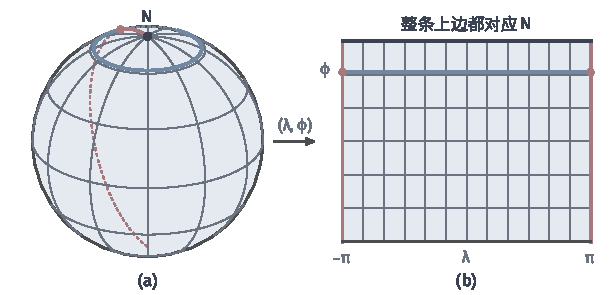
\includegraphics[width=104mm]{figures/04-spaces-measures-and-geometry/04-manifolds/matplotlib/mfd-sphere-latlong/figure.pdf}
  \caption{经纬度为什么覆盖不了整个球面。(a)球面上的经纬网，蓝色是高纬度的一条纬线，红色是取作接缝的经线$\lambda=\pm\pi$，背面部分画成虚线。(b)同一套网格在坐标矩形$(\lambda,\phi)$中的样子：北极一点被拉成整条上边，接缝被切成左右两条红边。球面上闭合的蓝色纬线在矩形中成为一条线段，两个红点是接缝上的同一点。}
  \label{fig:mfd-latlong}
\end{BookInlineFigure}

地图册解决这类问题的办法是用很多张局部地图拼起来：每张图只负责一块区域，在这块区域内干净地记录位置；相邻的图在重叠处约定怎样换算。圆周也是这样，一个角度足以定位一小段圆弧上的点，却无法不重复、不跳跃地记录整个圆。

这类对象的共同点是“局部像欧氏空间，整体未必是”。本章把这一认识写成\term{流形}（manifold）的定义，全程用圆、球面和环面三个具体对象走一遍：先用坐标图和换算规则定义流形，看局部欧氏结构带来哪些拓扑性质；再在流形上区分点、曲线、切向量和余切向量；然后建立随点变化的函数与场，最后用单位分解把局部构造拼成整体。

有一条线索贯穿全章：坐标是记录，不是对象。同一点、同一个速度、同一个读数在不同的图里有不同的数，这些数之间的换算规则由图之间的转移映射决定。凡是想在流形上定义一个概念，都要回答两个问题：它在一张图里怎么写，换一张图时结论是否不变。

本章只讨论同一个流形内部的对象。一个流形到另一个流形的映射怎样作用于点和切向量，是第~\ref{chap:manifold-maps}章的问题；两个流形何时光滑等价、何时构成子流形，见第~\ref{chap:manifold-relations}章。长度和角度需要额外选取度量，见第~\ref{chap:riemannian-geometry}章；微分形式与积分见第~\ref{chap:manifold-calculus}章。所用的拓扑概念沿用第~\ref{chap:topological-spaces}章。

\section{流形的定义}
\label{sec:mfd-definition}

曲线和曲面在微积分里常由参数化给出：圆是$\theta\mapsto(\cos\theta,\sin\theta)$的像，球面可以用经纬度参数化。参数化把一块欧氏区域送到对象上；反过来读，就是用几个实数记录对象上的一个点。图~\ref{fig:mfd-latlong}说明一张参数化通常只能照顾一部分，所以我们需要多张局部记录，并规定它们在重叠处怎样换算。

\subsection{坐标图与光滑相容性}
\label{sec:mfd-charts-compatibility}

先看圆周
\[
S^1=\{\bm y\in\mathbb R^2:\lVert\bm y\rVert_2=1\}.
\]
角度$\theta$可以记录圆上的点，但取值范围必须选一个长度为$2\pi$的开区间，否则同一点会有两个角度。取$(-\pi,\pi)$时，点$(-1,0)$没有角度；取$(0,2\pi)$时，点$(1,0)$没有角度。

为什么不用半开区间$[-\pi,\pi)$把漏掉的点补上？因为那样记录就不连续了：从下方逼近$(-1,0)$的点，角度趋于$-\pi$；从上方逼近的点，角度趋于$\pi$。圆上挨得很近的两点，记录却相距接近$2\pi$。单个角度无论怎样选，不是漏点就是断开，必须用至少两张局部记录才能覆盖整个圆。

\paragraph{坐标图与图册}
把“局部记录”说准确。它应当做两件事：把一块区域一一对应到欧氏空间的开集，并且不破坏邻近关系。这正是同胚的要求，即连续的双射且逆映射也连续。于是坐标接近当且仅当点接近，上面半开区间的毛病被排除在外。

\begin{definition}[坐标图与图册]
\label{def:mfd-chart}
设$M$是拓扑空间，$n\geq0$为整数。若$U\subseteq M$是开集，$\varphi:U\to\widehat U$是从$U$到某个开集$\widehat U\subseteq\mathbb R^n$的同胚，则称$(U,\varphi)$为$M$的一张$n$维\term{坐标图}（chart），$U$为它的定义域。对$p\in U$，称
\begin{equation}
\varphi(p)=(x_1(p),\ldots,x_n(p))
\label{eq:mfd-chart-coordinates}
\end{equation}
为$p$在这张图中的坐标，实值函数$x_i:U\to\mathbb R$称为坐标函数。定义域覆盖$M$的一族坐标图称为\term{图册}（atlas）。
\end{definition}

这些名词就是地图册的术语。表~\ref{tab:mfd-atlas-analogy}列出对应关系。类比在一处需要小心：真实的地图印在纸上有边缘和比例尺，坐标图只保证拓扑上的忠实，既不保持距离也不保持角度。距离要等到第~\ref{chap:riemannian-geometry}章选定度量之后才有意义。

\begin{BookInlineTable}
  \centering
  \begin{tabular}{ll}
    \toprule
    地图册 & 流形\\
    \midrule
    地球表面 & 空间$M$\\
    地面上的地点 & 点$p\in M$\\
    一张地图覆盖的区域 & 开集$U\subseteq M$\\
    把地点标到纸上的规则 & 同胚$\varphi:U\to\widehat U$\\
    地点在图上的位置 & 坐标$\varphi(p)$\\
    相邻两图的换算表 & 转移映射$\psi\circ\varphi^{-1}$\\
    \bottomrule
  \end{tabular}
  \caption{地图册与流形术语的对应。}
  \label{tab:mfd-atlas-analogy}
\end{BookInlineTable}

圆周的两张角度图组成一个图册：
\begin{equation}
\theta_1:S^1\setminus\{(-1,0)\}\to(-\pi,\pi),\qquad
\theta_2:S^1\setminus\{(1,0)\}\to(0,2\pi).
\label{eq:mfd-circle-charts}
\end{equation}
两者的逆都是$\theta\mapsto(\cos\theta,\sin\theta)$在相应区间上的限制。图的方向是“点到坐标”，参数化的方向是“坐标到点”，二者互为逆映射。图~\ref{fig:mfd-circle-charts}的(a)(b)画出了这两张图各漏掉哪一点。

\begin{BookInlineFigure}
  \centering
  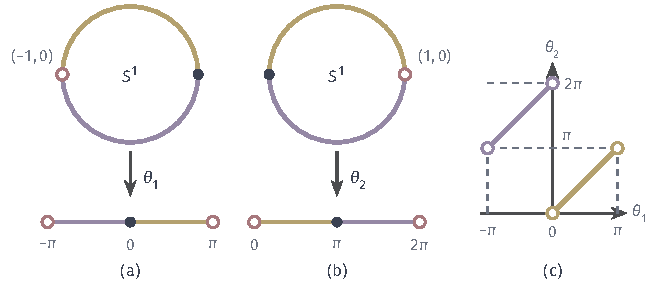
\includegraphics[width=111.605mm]{figures/04-spaces-measures-and-geometry/04-manifolds/tikz/mfd-circle-charts/figure.pdf}
  \caption{圆周的两张角度图及其转移映射。(a)(b)$\theta_1$漏掉$(-1,0)$，$\theta_2$漏掉$(1,0)$，漏掉的点用空心红圈表示。黄色弧是上半圆，紫色弧是下半圆，下方的开区间用相同颜色标出它们的坐标。(c)在重叠部分，$\theta_2$作为$\theta_1$的函数：上半圆上$\theta_2=\theta_1$（黄），下半圆上$\theta_2=\theta_1+2\pi$（紫），空心点表示这些坐标不属于重叠部分。}
  \label{fig:mfd-circle-charts}
\end{BookInlineFigure}

\paragraph{拓扑流形}
有了坐标图，就可以说一个空间“局部像$\mathbb R^n$”：每点都落在某张$n$维坐标图的定义域中。只要求这一条还不够，定义中要另加两个拓扑条件，用来排除两类病态空间。

\begin{definition}[拓扑流形]
\label{def:mfd-topological-manifold}
拓扑空间$M$称为$n$维\term{拓扑流形}（topological manifold），若它满足：
\begin{enumerate}
\item $M$是Hausdorff空间：任意两个不同点有互不相交的邻域；
\item $M$是第二可数的：拓扑有一个可数的基；
\item $M$局部欧氏：每个$p\in M$都属于某张$n$维坐标图的定义域。
\end{enumerate}
\end{definition}

Hausdorff条件保证点列的极限唯一。去掉它，就可能出现“双原点直线”：取两条实轴，把除原点以外的同名点粘在一起。所得空间每点附近都像一段实轴，局部欧氏条件成立；但两个原点没有不相交的邻域，点列$1/k$同时收敛到这两个原点。

第二可数条件排除“太大”的空间，例如不可数多条互不相交的实轴之并。这个条件有实际用途：它保证流形只有可数个连通分支，并能用一列紧集逐步穷竭，第~\ref{sec:mfd-partition-unity}节构造单位分解时就要用到。两个条件的一般讨论见第~\ref{chap:topological-spaces}章。

\paragraph{坐标变换与光滑相容}
拓扑流形只告诉我们哪些点彼此接近，还不能说一个函数“可微”。自然的想法是把函数写到坐标里再求导，但同一点可能落在两张图中，两张图的结论必须一致。这就要考察两套坐标之间的换算。

设$(U,\varphi)$与$(V,\psi)$是两张坐标图，$U\cap V\neq\varnothing$。先用$\varphi^{-1}$从第一张图回到流形上的点，再用$\psi$记到第二张图上，得到映射
\begin{equation}
\psi\circ\varphi^{-1}:\varphi(U\cap V)\to\psi(U\cap V).
\label{eq:mfd-transition}
\end{equation}
它把同一点在第一张图中的坐标换成第二张图中的坐标，称为\term{坐标变换}（transition map），也叫转移映射。

图~\ref{fig:mfd-chart-transition}画出了这个过程。要留意的是：$\varphi$和$\psi$的定义域在流形上，流形上一般没有微积分；而转移映射的定义域和值域都在欧氏空间里，可以用多元微积分判断它是否可微。这就是定义光滑结构的切入点。

\begin{BookInlineFigure}
  \centering
  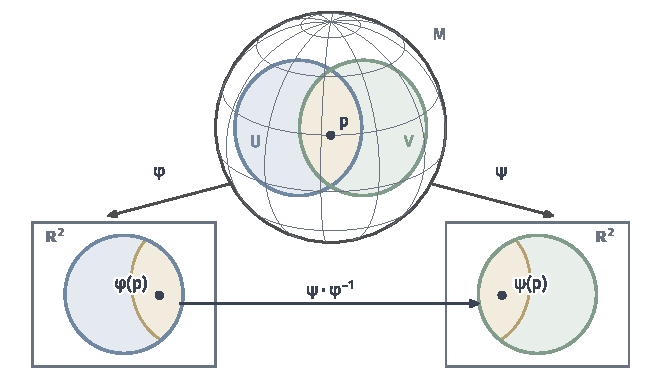
\includegraphics[width=112mm]{figures/04-spaces-measures-and-geometry/04-manifolds/matplotlib/mfd-chart-transition/figure.pdf}
  \caption{两张坐标图与转移映射。上方是球面上的两个球冠$U$（蓝）和$V$（绿），重叠部分为黄色。下方分别是向球冠中心切平面作正交投影得到的两张图。黄色区域是同一块重叠部分在两张图中的像，形状不同；转移映射$\psi\circ\varphi^{-1}$在两个黄色区域之间换算同一点$p$的坐标。}
  \label{fig:mfd-chart-transition}
\end{BookInlineFigure}

\begin{definition}[光滑相容与光滑结构]
\label{def:mfd-smooth-structure}
两张$n$维坐标图$(U,\varphi)$与$(V,\psi)$称为\term{光滑相容}（smoothly compatible）的，若$U\cap V=\varnothing$，或者坐标变换$\psi\circ\varphi^{-1}$与其逆$\varphi\circ\psi^{-1}$都是无穷次连续可微的。任意两张图都光滑相容的图册称为光滑图册。若一个光滑图册包含了所有与它的每张图都光滑相容的坐标图，就称它为极大光滑图册，也称$M$上的一个\term{光滑结构}（smooth structure）。带有光滑结构的拓扑流形称为\term{光滑流形}（smooth manifold）。
\end{definition}

本书说“光滑”都指无穷次连续可微。定义要求转移映射和它的逆都光滑，因为一个方向光滑不能保证另一方向也光滑，稍后的$x\mapsto x^3$就是例子。

极大图册听起来很大，实际使用时只需给出一个光滑图册：所有与它光滑相容的坐标图放在一起，就是包含它的唯一极大图册。需要检查的是这些新加入的图彼此也光滑相容。设$(V_1,\psi_1)$与$(V_2,\psi_2)$都与原图册相容，$q\in V_1\cap V_2$，取原图册中包含$q$的图$(U,\varphi)$。在$\psi_1(q)$附近可以经由$\varphi$中转：
\[
\psi_2\circ\psi_1^{-1}=(\psi_2\circ\varphi^{-1})\circ(\varphi\circ\psi_1^{-1}).
\]
右端两个因子都光滑，所以左端在$\psi_1(q)$附近光滑。光滑性是局部性质，逐点成立就在整个重叠区域成立。今后说“$M$的坐标图”，都指光滑结构中的坐标图。

\paragraph{例子：圆周}
现在把定义在圆周上走一遍。重叠区域是去掉$(\pm1,0)$后的两段开半圆。在上半圆，两个角度取值相同；在下半圆，$\theta_1$取$(-\pi,0)$中的值，$\theta_2$取$(\pi,2\pi)$中的值，二者相差$2\pi$。所以
\begin{equation}
\theta_2\circ\theta_1^{-1}(s)=
\begin{cases}
s, & s\in(0,\pi),\\
s+2\pi, & s\in(-\pi,0).
\end{cases}
\label{eq:mfd-circle-transition}
\end{equation}
图~\ref{fig:mfd-circle-charts}(c)是这个函数的图像，两段都是斜率为$1$的线段。

式~\eqref{eq:mfd-circle-transition}的定义域由两个不相交的开区间组成，在每段上都是平移，所以光滑，它的逆也是平移。于是这两张图构成光滑图册。坐标在下半圆跳过$2\pi$，只是记录方式的变化，圆本身并没有在那里断开。图中两段线段之间的空隙对应$\theta_1=0$，那里是$(1,0)$，它不在$\theta_2$的定义域内，所以不属于重叠部分。

\paragraph{例子：球面}
单位球面$S^2=\{\bm y\in\mathbb R^3:\lVert\bm y\rVert_2=1\}$上最方便的两张图来自\term{球极投影}（stereographic projection）。记北极$N=(0,0,1)$、南极$S=(0,0,-1)$。从北极向球面上的点$\bm y$作射线，射线与赤道平面的交点就是$\bm y$的坐标，如图~\ref{fig:mfd-stereographic}(a)所示。

下面把这个几何作图写成公式。过$N$和$\bm y$的直线上的点是$N+t(\bm y-N)$，它的第三个分量是$1+t(y_3-1)$。令第三个分量为零，得到
\[
t=\frac{1}{1-y_3}.
\]
代回前两个分量，得到北极图
\begin{equation}
\sigma_N(\bm y)=\frac{(y_1,y_2)}{1-y_3},\qquad \bm y\in S^2\setminus\{N\}.
\label{eq:mfd-stereographic-north}
\end{equation}

\begin{BookInlineFigure}
  \centering
  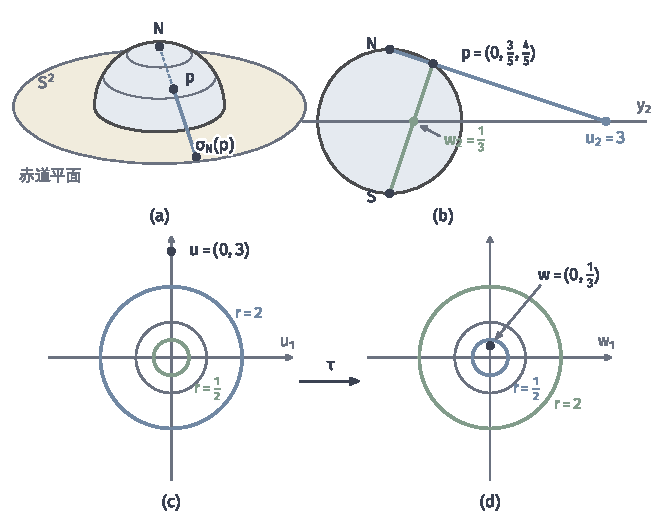
\includegraphics[width=112mm]{figures/04-spaces-measures-and-geometry/04-manifolds/matplotlib/mfd-stereographic/figure.pdf}
  \caption{球极投影及其转移映射。(a)从北极$N$过球面点$p$的射线交赤道平面（黄）于$\sigma_N(p)$，球内部分用虚线。(b)过$N$和$p=(0,\tfrac35,\tfrac45)$的竖直截面，蓝线给出北极图坐标$u_2=3$，绿线从南极给出南极图坐标$w_2=\tfrac13$。(c)(d)转移映射$\tau$把$\bm u$平面的圆周送到$\bm w$平面：半径$2$的蓝圆变成半径$\tfrac12$，半径$\tfrac12$的绿圆变成半径$2$，单位圆不变，$(0,3)$变成$(0,\tfrac13)$。}
  \label{fig:mfd-stereographic}
\end{BookInlineFigure}

反过来，给定$\bm u\in\mathbb R^2$，求球面上的对应点。记$\rho=\lVert\bm u\rVert_2^2$，点$\sigma_N^{-1}(\bm u)$在从$N$到$(\bm u,0)$的线段上，形如$(s\bm u,1-s)$。它在球面上，于是
\[
s^2\rho+(1-s)^2=1 .
\]
展开后约去$s\neq0$，得到$s(\rho+1)=2$。把$s=2/(\rho+1)$代回，就得到
\begin{equation}
\sigma_N^{-1}(\bm u)=\frac{\bigl(2u_1,\;2u_2,\;\rho-1\bigr)}{\rho+1},\qquad \rho=\lVert\bm u\rVert_2^2 .
\label{eq:mfd-stereographic-inverse}
\end{equation}
这是有理函数，$\sigma_N$与它的逆都连续，所以$\sigma_N$是$S^2\setminus\{N\}$到整个$\mathbb R^2$的同胚。同样地，从南极投影得到南极图
\begin{equation}
\sigma_S(\bm y)=\frac{(y_1,y_2)}{1+y_3},\qquad \bm y\in S^2\setminus\{S\}.
\label{eq:mfd-stereographic-south}
\end{equation}

两张图的重叠区域是去掉两极的球面，对应北极图中的$\mathbb R^2\setminus\{\bm0\}$。把式~\eqref{eq:mfd-stereographic-inverse}代入$\sigma_S$，先算分母：
\[
1+y_3=1+\frac{\rho-1}{\rho+1}=\frac{2\rho}{\rho+1}.
\]
前两个分量是$2\bm u/(\rho+1)$，相除后$\rho+1$消去，得到转移映射
\begin{equation}
\tau(\bm u)=\sigma_S\circ\sigma_N^{-1}(\bm u)=\frac{\bm u}{\lVert\bm u\rVert_2^2},\qquad \bm u\neq\bm 0.
\label{eq:mfd-stereographic-transition}
\end{equation}
这个映射叫反演：方向不变，半径变成倒数，图~\ref{fig:mfd-stereographic}(c)(d)就是它的样子。

$\tau$在$\mathbb R^2\setminus\{\bm0\}$上光滑，因为它是分母不为零的有理函数。再算$\tau\circ\tau$。由范数的计算，
\[
\lVert\tau(\bm u)\rVert_2^2=\frac{1}{\lVert\bm u\rVert_2^2},
\]
所以$\tau(\tau(\bm u))=\bm u$，$\tau$的逆就是它自己，同样光滑。于是$\{\sigma_N,\sigma_S\}$是$S^2$的光滑图册。球面作为$\mathbb R^3$的子空间，Hausdorff性与第二可数性都从$\mathbb R^3$继承，因此是二维光滑流形。

\paragraph{例子：欧氏开集与乘积}
最简单的光滑流形是$\mathbb R^n$本身，用恒等映射作唯一的图。它的任意开子集$W$也是光滑流形，图为恒等映射在$W$上的限制。更一般地，光滑流形的开子集用原有坐标图限制到其中，就成为同维光滑流形。

两个流形可以相乘。设$M$与$N$分别是$m$维与$n$维光滑流形，$(U,\varphi)$与$(V,\psi)$分别是二者的坐标图，令
\begin{equation}
(\varphi\times\psi)(p,q)=(\varphi(p),\psi(q))\in\mathbb R^{m+n}.
\label{eq:mfd-product-chart}
\end{equation}
这些乘积图覆盖$M\times N$。两张乘积图之间的坐标变换是两个坐标变换并排作用，各自光滑，所以并排后也光滑。乘积拓扑仍是Hausdorff且第二可数的，于是$M\times N$是$m+n$维光滑流形，称为\term{乘积流形}（product manifold）。

\term{环面}（torus）$T^2=S^1\times S^1$是最常用的乘积例子。一点由两个角度$(\theta,\phi)$记录，图~\ref{fig:mfd-torus-product}左边的正方形就是角度的取值范围，右边是同一个流形放进$\mathbb R^3$的样子，公式为
\[
\bigl((2+r\cos\phi)\cos\theta,\ (2+r\cos\phi)\sin\theta,\ r\sin\phi\bigr),\quad 0<r<2 .
\]
这只是外观，环面作为乘积流形并不需要$\mathbb R^3$。正方形的上下边是同一个圆，左右边也是同一个圆，把两组对边粘起来就得到环面。

\begin{BookInlineFigure}
  \centering
  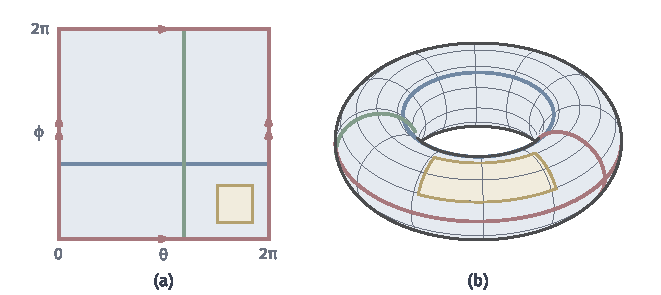
\includegraphics[width=112mm]{figures/04-spaces-measures-and-geometry/04-manifolds/matplotlib/mfd-torus-product/figure.pdf}
  \caption{环面$S^1\times S^1$的角度坐标。(a)角度正方形，带箭头的红色对边两两等同；黄色矩形是一小块坐标区域，蓝线$\phi=$常数，绿线$\theta=$常数。(b)嵌入$\mathbb R^3$的环面（$r=0.82$）上同一块区域和同样两条圈，红色两条圈是$\phi=0$和$\theta=0$的接缝。灰线为角度网格。}
  \label{fig:mfd-torus-product}
\end{BookInlineFigure}

圆周的两张图做乘积，就得到环面的四张图：$\theta_a\times\theta_b$，$a,b\in\{1,2\}$。以圆周上$\theta_1=1$和$\theta_1=-2$对应的两点组成的乘积点为例，它在四张图中的坐标分别是
\[
(1,-2),\quad (1,-2+2\pi),\quad (1,-2),\quad (1,-2+2\pi),
\]
依次对应$(a,b)=(1,1),(1,2),(2,1),(2,2)$，其中第一个角度$1\in(0,\pi)$两图相同，第二个角度$-2\in(-\pi,0)$需要加$2\pi$。这正是式~\eqref{eq:mfd-circle-transition}在两个分量上分别作用。

\paragraph{相容性是附加的选择}
光滑相容不是自动成立的。在$\mathbb R$上，$\chi(x)=x^3$是$\mathbb R$到$\mathbb R$的同胚，因而是一张合法的拓扑坐标图。它与恒等图之间的两个转移映射是
\[
\chi\circ\mathrm{id}^{-1}(x)=x^3,\qquad \mathrm{id}\circ\chi^{-1}(y)=y^{1/3}.
\]
前者光滑，后者在原点不可微。所以$\chi$与恒等图不光滑相容。

$\{\chi\}$单独也是一个光滑图册，它决定了$\mathbb R$上另一个光滑结构。在这个结构下，函数$f(x)=x$的坐标表示是$f\circ\chi^{-1}(y)=y^{1/3}$，不再光滑。可见同一个拓扑空间上的光滑性取决于所选的光滑结构。后文默认使用标准结构，两种结构之间能否用光滑映射互相转换，留到第~\ref{chap:manifold-relations}章讨论。

\paragraph{维数}
定义中的$n$对每张图都相同。假如允许不同维数的图，光滑情形也不会出现矛盾。设$m$维与$n$维的两张图重叠，$\tau$是转移映射，$\tau^{-1}$是逆，对$\tau^{-1}\circ\tau=\mathrm{id}$和$\tau\circ\tau^{-1}=\mathrm{id}$用链式法则，得到
\[
\bm J_{\tau^{-1}}\bm J_{\tau}=\bm I_m,\qquad
\bm J_{\tau}\bm J_{\tau^{-1}}=\bm I_n .
\]
一个$n\times m$矩阵既有左逆也有右逆，就是可逆方阵，所以$m=n$。多元链式法则可参考\BookChapterRef{chap:multivariate-differentiation}{卷二第17章“多元函数微分”}。对拓扑流形，同样的结论依赖区域不变性定理，证明需要代数拓扑的工具，篇幅较长，这里只使用结论。

\subsection{带边界的流形}
\label{sec:mfd-boundary}

闭圆盘
\[
\overline{B}{}^2=\{\bm y\in\mathbb R^2:\lVert\bm y\rVert_2\leq1\}
\]
不是上面意义的流形：圆周上的点无论取多小的邻域，邻域都只在圆盘一侧，形状是半个圆盘，而不是一个开圆盘。区间$[0,1]$的端点、半球面的赤道也是这样。这些对象并不病态，只是局部模型要放宽：从欧氏开集放宽到半空间。

\paragraph{半空间模型}
记$n\geq1$维闭上半空间及其边界为
\begin{equation}
\mathbb H^n=\{\bm x\in\mathbb R^n:x_n\geq0\},\qquad
\partial\mathbb H^n=\{\bm x\in\mathbb R^n:x_n=0\}.
\label{eq:mfd-halfspace}
\end{equation}
$\mathbb H^n$的开子集指它与$\mathbb R^n$中某个开集的交。例如半圆盘$\{\bm x\in\mathbb H^2:\lVert\bm x\rVert_2<1\}$含有底边上的点，它是$\mathbb H^2$的开子集，却不是$\mathbb R^2$的开集。

图~\ref{fig:mfd-boundary-models}比较了三种局部情形。内点(a)的邻域是开圆盘，模型是$\mathbb R^2$的开集；边界点(b)的邻域是半个圆盘，模型是$\mathbb H^2$的开子集；正方形的角点(c)的邻域在平面坐标中是象限，不在这两种模型之内，后面专门讨论。

\begin{BookInlineFigure}
  \centering
  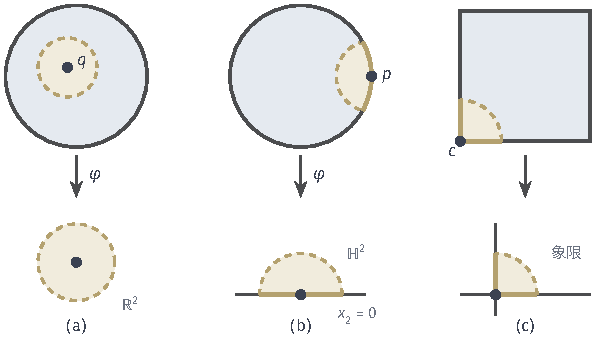
\includegraphics[width=100.856mm]{figures/04-spaces-measures-and-geometry/04-manifolds/tikz/mfd-boundary-models/figure.pdf}
  \caption{三种局部模型。上排是闭圆盘或闭正方形中的一个小邻域（黄），下排是它在坐标图中的像。(a)内点$q$的邻域对应$\mathbb R^2$的开圆盘，虚线表示边不含在内。(b)边界点$p$的邻域对应$\mathbb H^2$的半圆盘，粗黄线是位于边界上的部分，含在邻域内。(c)角点$c$的邻域在平面坐标中是象限，不是半圆盘。}
  \label{fig:mfd-boundary-models}
\end{BookInlineFigure}

\begin{definition}[带边界的拓扑流形]
\label{def:mfd-manifold-with-boundary}
Hausdorff且第二可数的拓扑空间$M$称为$n$维\term{带边界流形}（manifold with boundary），若每个$p\in M$都有开邻域$U$和从$U$到$\mathbb H^n$的某个开子集的同胚$\varphi$。若某张这样的图把$p$送到$\partial\mathbb H^n$中，称$p$为\term{边界点}（boundary point）；若某张图把$p$送到$\{x_n>0\}$中，称$p$为内点。全部边界点组成的集合记为$\partial M$。
\end{definition}

$\{x_n>0\}$本身是$\mathbb R^n$的开集，所以内点附近的局部模型与无边界情形相同。没有边界点的带边界流形就是前面的流形，为了区分，后者也称无边界流形。

\paragraph{半空间上的光滑性}
要定义带边界流形的光滑结构，先得说清半空间开子集上的映射何时光滑。边界点处只有一侧的值，双侧差商算不了偏导数。约定的做法是借助延拓：若映射在边界点附近能光滑地延拓到一个完整的欧氏开邻域，就称它在那里光滑。

\begin{definition}[半空间开子集上的光滑映射]
\label{def:mfd-smooth-halfspace}
设$A\subseteq\mathbb H^n$是开子集，$F:A\to\mathbb R^k$。若对每个$\bm a\in A$，都有$\mathbb R^n$中的开邻域$W\ni\bm a$与光滑映射$\widetilde F:W\to\mathbb R^k$，使$\widetilde F=F$在$W\cap A$上成立，则称$F$光滑。
\end{definition}

延拓不唯一，但边界点处各阶导数与延拓的选择无关。原因在于内点可以逼近边界点：任意边界点$\bm a$都是内点$\bm a+t\bm e_n$（$t\to0^+$）的极限，延拓在这些内点处的导数就是$F$本身的导数，而$\widetilde F$的各阶导数连续，所以在$\bm a$处的值等于内侧导数的极限，由$F$决定。

有了这一定义，带边界流形的光滑相容性、光滑图册和光滑结构可以逐字照搬定义~\ref{def:mfd-smooth-structure}，只是把坐标变换理解为$\mathbb H^n$开子集之间的映射。

\paragraph{内点与边界点不会混淆}
定义~\ref{def:mfd-manifold-with-boundary}说的是“某张图”把点送到边界，于是要问：会不会有一点在一张图中是边界点，在另一张中是内点？直观上，内点四周都有路可走，边界点只有一侧。下面用Jacobian矩阵把这个直观变成证明。

\begin{theorem}[边界点的坐标无关性]
\label{thm:mfd-boundary-invariance}
设$M$是光滑带边界流形，$p\in M$。若某张光滑坐标图把$p$送到$\partial\mathbb H^n$中，则每张包含$p$的光滑坐标图都把$p$送到$\partial\mathbb H^n$中。
\end{theorem}

\begin{proof}
用反证法。设图$(V,\psi)$把$p$送到边界，图$(U,\varphi)$把$p$送到$\{x_n>0\}$。取$\varphi(p)$在$\mathbb R^n$中的开球$W$，使$W\subseteq\varphi(U\cap V)$，这一步用到$\varphi(p)$是内点。记$\tau=\psi\circ\varphi^{-1}$，它在$W$上光滑。

它的逆$\varphi\circ\psi^{-1}$在$\psi(p)$附近光滑，即在$\psi(p)$的欧氏邻域上有光滑延拓$\widetilde\tau$。在$\varphi(p)$附近，$\widetilde\tau\circ\tau=\mathrm{id}$，对它求导得到
\[
\bm J_{\widetilde\tau}(\psi(p))\,\bm J_\tau(\varphi(p))=\bm I_n .
\]
于是$\bm J_\tau(\varphi(p))$可逆。

由局部反函数定理，$\tau$把$\varphi(p)$的某个开邻域映成$\psi(p)$在$\mathbb R^n$中的一个开邻域，该定理可参考\BookChapterRef{chap:implicit-inverse-functions}{卷二第19章“隐函数与反函数”}。可是$\tau$的值都在$\mathbb H^n$中，而$\psi(p)$的最后一个坐标为零，它的任何欧氏开邻域都含有$x_n<0$的点。这一矛盾说明假设不成立。
\end{proof}

对拓扑带边界流形，同样的结论也成立，但证明需要同调等工具，读者可查阅代数拓扑的教材。今后谈论$\partial M$时，总是在光滑情形下进行。

\paragraph{边界本身的结构}
边界点处的坐标图限制到边界上，给出边界的局部坐标。设$(U,\varphi)$是包含边界点的图，由定理~\ref{thm:mfd-boundary-invariance}，
\[
\varphi(U\cap\partial M)=\varphi(U)\cap\partial\mathbb H^n .
\]
把$\partial\mathbb H^n$等同于$\mathbb R^{n-1}$，限制映射$\varphi|_{U\cap\partial M}$就是$\partial M$的一张$n-1$维坐标图。两张这样的图之间的坐标变换是原坐标变换在边界上的限制，仍然光滑。所以$\partial M$是$n-1$维无边界光滑流形。

用闭圆盘检验这些定义。内部的点用平面坐标的限制作图。边界点用极坐标$(\theta,s)$作图，其中$s=1-r\geq0$，例如在$(1,0)$附近取
\[
\theta\in(-\tfrac{\pi}{2},\tfrac{\pi}{2}),\qquad s\in[0,\tfrac12).
\]
在这张图中，圆周恰好对应$s=0$，所以$\partial\overline B{}^2=S^1$，它是一维无边界流形。区间$[0,1]$是一维带边界流形，边界由两个端点组成，是零维流形。

\paragraph{角点不是同一种光滑边界}
闭正方形$[0,1]^2$同胚于闭圆盘，所以是拓扑带边界流形。但在角点处，平面坐标给出的局部模型是象限$\{x_1\geq0,x_2\geq0\}$，而不是半平面。

能否换一张图把象限摊平？把平面看作复平面，$z\mapsto z^2$确实把象限映成上半平面。可它的逆$z\mapsto\sqrt z$在原点不可微，所以这样得到的坐标与平面原有坐标不光滑相容。这说明如果沿用平面坐标所定义的光滑性，角点不能纳入光滑带边界流形的框架。这类对象需要另行建立带角流形的理论，本书不作讨论。

\section{流形的拓扑性质}
\label{sec:mfd-topology}

流形首先是拓扑空间，第~\ref{chap:topological-spaces}章关于连通性与紧性的一般结论都适用。这里只问一个问题：每点附近像欧氏空间这一局部条件，会给整体性质带来什么新结论？下面看两处：连通与路径连通在流形上不再需要区分，紧流形可以用有限张坐标图覆盖。这些结论对带边界流形同样成立，因为半空间中的半球也像欧氏球那样可以用线段连接。

\subsection{连通与路径连通}
\label{sec:mfd-connectedness}

回忆两种概念的区别：连通指空间不能分成两个不相交的非空开集，路径连通指任意两点都能用连续路径连接。路径连通总蕴含连通，反过来一般不成立。

典型反例是拓扑学家的正弦曲线，即曲线$\{(y_1,\sin(1/y_1)):0<y_1\leq1\}$与竖直线段$\{0\}\times[-1,1]$的并，如图~\ref{fig:mfd-connected-sine}(b)所示。曲线越靠近竖直线段振荡越快，竖线上每一点都是曲线上点的极限，所以两部分不能被开集分开，集合连通。但从竖直线段上的点出发，没有连续路径能走到曲线部分。

\begin{BookInlineFigure}
  \centering
  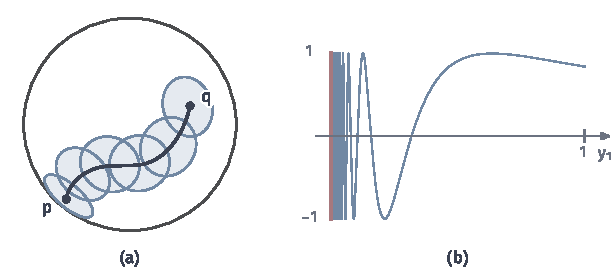
\includegraphics[width=104mm]{figures/04-spaces-measures-and-geometry/04-manifolds/matplotlib/mfd-connected-sine/figure.pdf}
  \caption{局部的线段连接与它失效的情形。(a)球面上连接$p,q$的路径（黑线）由一串相互重叠的坐标球（蓝）接力完成，每个坐标球内部都能用线段走通。(b)拓扑学家的正弦曲线$y_2=\sin(1/y_1)$（蓝）与竖直线段（红）的并。竖线上任意一点的小邻域都含有无穷多段互不相连的弧，所以这里没有路径连通的邻域。}
  \label{fig:mfd-connected-sine}
\end{BookInlineFigure}

\paragraph{局部路径连通}
流形上情况要好得多，因为每点附近都是欧氏的。取包含$p$的坐标图$(U,\varphi)$，在$\varphi(U)$中取以$\varphi(p)$为中心的开球$B$，称$\varphi^{-1}(B)$为\term{坐标球}（coordinate ball）。

球中任意两点$\bm a,\bm b$用线段$t\mapsto(1-t)\bm a+t\bm b$连接，线段留在球内，再用$\varphi^{-1}$送回流形，就得到坐标球内连接两点的连续路径。带边界的情形用半球代替球，半球同样是凸集，线段仍留在其中。于是每点都有任意小的路径连通邻域，这一性质称为\term{局部路径连通}（locally path-connected）。

\begin{theorem}[流形上连通与路径连通等价]
\label{thm:mfd-connected-path-connected}
设$M$是拓扑流形或带边界拓扑流形。则$M$连通当且仅当$M$路径连通。更一般地，$M$的每个路径分支都是既开又闭的集合，并且路径分支与连通分支一致。
\end{theorem}

证明的想法如图~\ref{fig:mfd-connected-sine}(a)：从一点出发能走到的地方，每个点周围都还有一个坐标球能走，所以这个范围不会有“边缘”。

\begin{proof}
设$C$是一个路径分支，即与某点有路径相连的全部点组成的集合。对$q\in C$，取$q$的坐标球$B_q$。$B_q$中每一点都能先连到$q$，再从$q$连到$C$的起点，所以$B_q\subseteq C$，$C$是开集。

不同路径分支互不相交，$C$的补集是其余路径分支的并，也是开集，所以$C$又是闭集。若$M$连通，它唯一的非空既开又闭子集是自身，于是$C=M$，$M$路径连通。反方向是一般拓扑空间中已有的结论。

最后比较两种分支。路径分支$C$路径连通，因而连通，含于某个连通分支$D$。$C$在$D$中既开又闭且非空，$D$连通，所以$C=D$。
\end{proof}

证明只用到“每点有路径连通的邻域”。正弦曲线在竖直线段上的点处缺少这样的邻域，这也说明它不是流形，不能拿来否定定理~\ref{thm:mfd-connected-path-connected}。

\paragraph{连通分支的个数}
每个连通分支是开集，因而本身也是同维流形。第二可数性还限制了分支的个数：每个分支都含有可数基中的某个非空基元素，不同分支所含的基元素不同，所以分支至多可数。

例如双曲线$\{\bm y\in\mathbb R^2:y_2^2-y_1^2=1\}$有上下两个连通分支，每个分支同胚于$\mathbb R$。连通分支数这一整体信息后来由零维同调记录，见第~\ref{chap:homology}章。

\subsection{紧性}
\label{sec:mfd-compactness}

紧空间的任意开覆盖都有有限子覆盖，紧空间上的连续实值函数取得最大值和最小值。这两条在流形上有直接用途。前者让我们只用有限张坐标图处理整个紧流形；后者保证球面上的高度函数$\bm y\mapsto y_3$在某些点达到最高和最低，第~\ref{sec:mfd-smooth-functions}小节将用坐标验证这些点处微分为零。

\paragraph{有限个坐标图}
所有坐标图的定义域组成$M$的一个开覆盖。若$M$紧，就能从中选出有限张图覆盖$M$。圆周用两张图，球面用两张球极投影图，环面用四张乘积图。很多构造先在每张图上局部完成，再把结果拼起来；图的张数有限时，拼接中的求和、取最大值等操作都只涉及有限项。

\paragraph{有限张图不等于一张图}
紧性只给出有限张图，不能推出一张图就够。实际上，正维数的非空紧无边界流形一定不能由单张坐标图覆盖。

证明很短。假设$\varphi:M\to\widehat U$是覆盖整个$M$的坐标图。$\widehat U=\varphi(M)$是紧集的连续像，因而是$\mathbb R^n$中的有界闭集。它又是非空开集，于是是$\mathbb R^n$中非空的既开又闭子集。$\mathbb R^n$连通，所以$\widehat U=\mathbb R^n$，这与有界矛盾。

因此圆周、球面和环面都至少需要两张图。本章开头经纬度在两极失效，问题不在经纬度选得不好，而在于球面的紧性使任何单张坐标图都不可能覆盖全部。

反过来，非紧流形有时一张图就够，例如$\mathbb R^n$。双曲线虽有两个分支，也能用一张图覆盖：在上支令$\varphi(\bm y)=\arctan y_1$，在下支令$\varphi(\bm y)=\arctan y_1+4$，两支分别被送到不相交的开区间$(-\pi/2,\pi/2)$与$(4-\pi/2,4+\pi/2)$。欧氏开集本来就不必连通。单张图能否覆盖整个流形，等于问整个流形能否同胚于一个欧氏开集，紧性只是排除这种可能的一个充分原因。

\section{点与曲线}
\label{sec:mfd-points-curves}

流形是一个整体空间，它的元素是点。在欧氏空间中，点与它的坐标几乎不加区分；在流形上，坐标只是某张局部地图对点的记录，换一张图记录就变。先弄清哪些运算属于点、哪些只属于坐标，再用参数曲线描述点随参数的连续变化。

\subsection{点的坐标表示}
\label{sec:mfd-point-coordinates}

取球面上的点$p=(0,\tfrac35,\tfrac45)$，它就是图~\ref{fig:mfd-stereographic}(b)中的那一点。按式~\eqref{eq:mfd-stereographic-north}，分母是$1-\tfrac45=\tfrac15$，所以北极图坐标是
\[
\sigma_N(p)=\frac{(0,\tfrac35)}{1/5}=(0,3).
\]
按式~\eqref{eq:mfd-stereographic-south}，分母是$1+\tfrac45=\tfrac95$，所以南极图坐标是
\[
\sigma_S(p)=\frac{(0,\tfrac35)}{9/5}=(0,\tfrac13).
\]
两组数不同，记录的是同一个点。代入转移映射\eqref{eq:mfd-stereographic-transition}核对：$\tau(0,3)=(0,3)/9=(0,\tfrac13)$，正好对上。

\paragraph{坐标运算不定义点的运算}
坐标是$\mathbb R^2$中的向量，可以相加。但“两个点的坐标之和”在不同图中对应不同的点。再取$q=(0,-\tfrac35,\tfrac45)$，它在两张图中的坐标分别是$(0,-3)$与$(0,-\tfrac13)$。

两点的坐标相加，在北极图和南极图里都得到$(0,0)$。但$(0,0)$在两张图中代表不同的点：
\[
\sigma_N^{-1}(0,0)=(0,0,-1)=S,\qquad
\sigma_S^{-1}(0,0)=(0,0,1)=N .
\]
同样的两点，用北极图相加得到南极，用南极图相加得到北极。

所以坐标的加法依赖所用的图，不是流形上点的运算。球面上本来也没有自然的加法：$p,q$作为$\mathbb R^3$中向量的和是$(0,0,\tfrac85)$，它根本不在球面上。今后凡是在坐标中做线性运算，都要说明它在哪张图中进行，所得结论是否与图的选择无关。

\paragraph{邻域与点列收敛}
点的接近关系由流形的拓扑决定，坐标图把它如实翻译成欧氏空间中的接近。设$(U,\varphi)$是包含$p$的坐标图。$U$是$p$的开邻域，$\varphi$是同胚，所以$p$在$U$中的邻域与$\varphi(p)$在$\varphi(U)$中的邻域一一对应。点列收敛因此可以逐点翻译成坐标收敛。

\begin{lemma}[点列收敛的坐标判别]
\label{lem:mfd-sequence-convergence}
设$(U,\varphi)$是包含$p$的坐标图，$(p_k)$是$M$中的点列。则$p_k\to p$当且仅当存在$K$，使$k\geq K$时$p_k\in U$，并且$\varphi(p_k)\to\varphi(p)$。
\end{lemma}

\begin{proof}
若$p_k\to p$，因$U$是$p$的开邻域，从某项起$p_k\in U$；$\varphi$连续，所以$\varphi(p_k)\to\varphi(p)$。反过来，若从某项起$p_k\in U$且坐标收敛，因$\varphi^{-1}$连续，$p_k=\varphi^{-1}(\varphi(p_k))\to p$。
\end{proof}

这个判别不依赖图的选择。若$(V,\psi)$是另一张包含$p$的图，从某项起$p_k\in U\cap V$，坐标变换$\psi\circ\varphi^{-1}$连续，所以一张图中的坐标收敛推出另一张图中的坐标收敛。光滑相容比连续更强，它还保证坐标的变化速度在两张图中能够换算，这一点在曲线速度中用到。

引理要求$p_k$最终落入$U$，这一条不能省。圆周上取$p=(1,0)$，令
\[
p_k=\bigl(\cos\tfrac{(-1)^k}{k},\ \sin\tfrac{(-1)^k}{k}\bigr).
\]
用$\theta_1$看，坐标$(-1)^k/k\to0$，所以$p_k\to p$。换用$\theta_2$，偶数项的坐标是$1/k$，奇数项的坐标是$2\pi-1/k$，在区间两端来回跳动。这是因为$p$不在$\theta_2$的定义域内，不说明点列不收敛。

\subsection{光滑曲线}
\label{sec:mfd-smooth-curves}

一个质点在圆周上匀速转动，时刻$t$的位置是$\gamma(t)=(\cos t,\sin t)$。这里的对象是映射$t\mapsto\gamma(t)$，而不只是它经过的点集：同样转过整个圆，转得快慢不同、方向不同，都是不同的运动。

\paragraph{曲线及其光滑性}
曲线是从参数区间到流形的映射。判断它是否光滑，仍然借助坐标：在每一时刻附近，用一张包含当前位置的图记录位置，得到一条普通的欧氏坐标曲线。

\begin{definition}[光滑曲线]
\label{def:mfd-smooth-curve}
设$I\subseteq\mathbb R$是区间，$\gamma:I\to M$连续。若对每个$t_0\in I$和每张包含$\gamma(t_0)$的坐标图$(U,\varphi)$，坐标曲线$\varphi\circ\gamma$在$t_0$附近光滑，则称$\gamma$为\term{光滑曲线}（smooth curve）。$I$含端点时，端点处按单侧导数理解。
\end{definition}

$\gamma$连续，所以$\gamma^{-1}(U)$是包含$t_0$的开集，坐标曲线在$t_0$附近确有定义。定义要求对每张图都成立，但只需检查一张。若$(V,\psi)$是另一张包含$\gamma(t_0)$的图，则在$t_0$附近
\[
\psi\circ\gamma=(\psi\circ\varphi^{-1})\circ(\varphi\circ\gamma).
\]
转移映射光滑，光滑映射的复合仍光滑，所以$\varphi\circ\gamma$光滑推出$\psi\circ\gamma$光滑。对上式用链式法则，就得到两张图中坐标速度的关系：
\begin{equation}
(\psi\circ\gamma)'(t_0)=\bm J\,(\varphi\circ\gamma)'(t_0),\quad
\bm J=\bm J_{\psi\circ\varphi^{-1}}\bigl(\varphi(\gamma(t_0))\bigr).
\label{eq:mfd-curve-velocity-change}
\end{equation}
两张图记录的速度分量不同，但由转移映射的Jacobian矩阵确定地换算。下一节把这种“由一族记录和一条换算规则共同确定的对象”定义为切向量。

\paragraph{圆周上的例子}
在角度图$\theta_1$中，$\gamma(t)=(\cos t,\sin t)$对$t\in(-\pi,\pi)$的坐标曲线是$\theta_1(\gamma(t))=t$；在$\theta_2$中，对$t\in(0,2\pi)$是$\theta_2(\gamma(t))=t$，其余时刻差$2\pi$的整数倍。各段都是一次函数，所以$\gamma$在整条实轴上光滑，两张图记录的速度都是$1$。这与式~\eqref{eq:mfd-curve-velocity-change}一致，因为转移映射是平移，Jacobian为$1$。

\paragraph{曲线与它的像}
同一个像可以由许多不同的曲线描出。曲线$\gamma_2(t)=(\cos2t,\sin2t)$也绕整个圆走，但在角度图中速度为$2$。$\gamma_3(t)=(\cos t^3,\sin t^3)$也绕圆运动，坐标曲线$t^3$光滑，可在$t=0$处速度为零，质点在那一刻停了一下。图~\ref{fig:mfd-curves-parametrization}(a)比较了这三条坐标曲线。

\begin{BookInlineFigure}
  \centering
  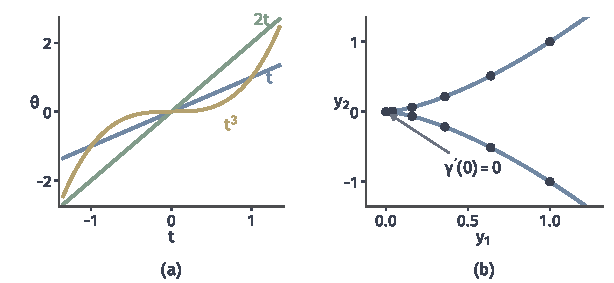
\includegraphics[width=104mm]{figures/04-spaces-measures-and-geometry/04-manifolds/matplotlib/mfd-curves-parametrization/figure.pdf}
  \caption{曲线是映射，不是点集。(a)圆周上三条曲线在角度图中的坐标曲线$\theta=t,2t,t^3$，三者经过相同的点，速度不同，$t^3$在$t=0$处速度为零。(b)平面曲线$\gamma(t)=(t^2,t^3)$的像，黑点是$t=-1,-0.8,\ldots,1$时的位置。分量都是多项式，映射光滑，像却在原点有尖点，那一刻速度恰好为零，黑点也在此处聚拢。}
  \label{fig:mfd-curves-parametrization}
\end{BookInlineFigure}

反过来，映射光滑，像却可以不光滑。平面曲线$\gamma(t)=(t^2,t^3)$的两个分量都是多项式，所以是光滑曲线。计算它的速度：
\[
\gamma'(t)=(2t,\ 3t^2),\qquad \gamma'(0)=(0,0).
\]
它的像$\{(y_1,y_2):y_1^3=y_2^2\}$在原点有尖点，见图~\ref{fig:mfd-curves-parametrization}(b)。尖点处速度恰好为零，所以光滑映射的像才可能在那里拐出尖角。因此“光滑曲线”说的是映射，不是点集；曲线的像能否成为一个光滑子流形，是第~\ref{chap:manifold-relations}章的问题。

\paragraph{边界点处的曲线}
在带边界流形中，曲线可以停在边界上，也可以从边界出发进入内部。闭圆盘中$\gamma(t)=(1-t,0)$，$t\in[0,1)$，从边界点$(1,0)$出发向内运动，只能取$t\geq0$；若取$t<0$，点会离开圆盘。所以过边界点的光滑曲线一般只能是单侧的。

下一节先在内点处用双侧曲线的速度建立切向量。边界点处只收集单侧曲线的速度，得到的是半个空间，而不是线性空间，那里的切空间要换一种方式定义，见第~\ref{sec:mfd-tangent-space}小节。

\section{切空间与余切空间}
\label{sec:mfd-tangent-cotangent}

球面放在$\mathbb R^3$中时，曲线的速度可以直接在$\mathbb R^3$中求导，得到一个与球面相切的向量。一般流形没有现成的外部空间，速度必须用流形自身的语言描述。上一节已经看到，同一速度在两张图中的分量由坐标变换的Jacobian矩阵换算。本节先在内点处把速度定义为曲线的等价类，组成切空间，再用一族坐标记录处理边界点。随后把对切向量的线性读数组织成余切空间，比较两者在换图时的不同变换规则。

\subsection{切空间}
\label{sec:mfd-tangent-space}

\paragraph{内点处的曲线速度}
设$p$是$M$的内点。经过$p$的光滑曲线$\gamma:(-\varepsilon,\varepsilon)\to M$，$\gamma(0)=p$，在一张包含$p$的图$(U,\varphi)$中有坐标速度$(\varphi\circ\gamma)'(0)\in\mathbb R^n$。两条曲线可能形状完全不同，却在$p$处有相同的坐标速度；就“此刻往哪里、以多快的速度运动”而言，它们没有区别。

\begin{definition}[切向量与切空间]
\label{def:mfd-tangent-space}
设$p$是光滑流形$M$的内点，$(U,\varphi)$是包含$p$的坐标图。对经过$p$的两条光滑曲线$\gamma_1,\gamma_2$，若$(\varphi\circ\gamma_1)'(0)=(\varphi\circ\gamma_2)'(0)$，则称二者在$p$处等价。等价类$[\gamma]$称为$p$处的\term{切向量}（tangent vector），也记作$\gamma'(0)$；全体切向量组成的集合$T_pM$称为$M$在$p$处的\term{切空间}（tangent space）。
\end{definition}

定义中用了一张特定的图，但等价关系与图无关：若在$\varphi$中坐标速度相同，由式\eqref{eq:mfd-curve-velocity-change}，在另一张图$\psi$中二者的坐标速度都等于同一个矩阵乘以同一个向量，仍然相同。

\paragraph{切空间的线性结构}
切向量是等价类，本来没有加法。下面借用坐标记录把$\mathbb R^n$的线性结构搬过来，并说明搬来的结构与所用的图无关。

\begin{theorem}[切空间是$n$维线性空间]
\label{thm:mfd-tangent-linear}
设$p$是$n$维光滑流形$M$的内点，$(U,\varphi)$是包含$p$的坐标图。映射
\[
\Theta_\varphi:T_pM\to\mathbb R^n,\qquad [\gamma]\mapsto(\varphi\circ\gamma)'(0)
\]
是双射。用它把$\mathbb R^n$的加法与数乘搬到$T_pM$上，所得线性结构与$\varphi$的选择无关，$T_pM$是$n$维实线性空间。
\end{theorem}

\begin{proof}
单射直接来自等价关系的定义。为证满射，任取$\bm v\in\mathbb R^n$。$p$是内点，$\varphi(U)$是包含$\varphi(p)$的欧氏开集，所以$t$足够小时$\varphi(p)+t\bm v\in\varphi(U)$，曲线$\gamma(t)=\varphi^{-1}(\varphi(p)+t\bm v)$有定义且光滑，坐标速度为$\bm v$。

若$(V,\psi)$是另一张包含$p$的图，式\eqref{eq:mfd-curve-velocity-change}说明$\Theta_\psi=\bm J\,\Theta_\varphi$，其中$\bm J=\bm J_{\psi\circ\varphi^{-1}}(\varphi(p))$是可逆矩阵。可逆线性映射保持线性组合，所以按$\Theta_\varphi$规定的$a[\gamma_1]+b[\gamma_2]$，在$\Theta_\psi$下的记录是$a\Theta_\psi[\gamma_1]+b\Theta_\psi[\gamma_2]$，两张图规定的运算相同。
\end{proof}

\paragraph{坐标基与变换规则}
$\mathbb R^n$的标准基$\bm e_1,\ldots,\bm e_n$在$\Theta_\varphi^{-1}$下给出$T_pM$的一组基，记为
\[
\left.\frac{\partial}{\partial x_i}\right|_p=\Theta_\varphi^{-1}(\bm e_i),\qquad i=1,\ldots,n,
\]
称为\term{坐标基}（coordinate basis），简记为$\partial_i|_p$。它就是第$i$条坐标线$t\mapsto\varphi^{-1}(\varphi(p)+t\bm e_i)$的速度。任一切向量写成$\bm v=\sum_i v_i\,\partial_i|_p$，系数$(v_1,\ldots,v_n)=\Theta_\varphi(\bm v)$称为它在这张图中的分量。

换一张图$\psi$，坐标记为$\tilde x_1,\ldots,\tilde x_n$，同一切向量的分量变为
\begin{equation}
\tilde v_k=\sum_{j=1}^n\frac{\partial\tilde x_k}{\partial x_j}(\varphi(p))\,v_j,
\qquad\text{即}\qquad
\left.\frac{\partial}{\partial x_j}\right|_p=\sum_{k=1}^n\frac{\partial\tilde x_k}{\partial x_j}(\varphi(p))\left.\frac{\partial}{\partial\tilde x_k}\right|_p,
\label{eq:mfd-tangent-change}
\end{equation}
其中$\partial\tilde x_k/\partial x_j$是坐标变换$\psi\circ\varphi^{-1}$的Jacobian矩阵的元素。左式说明分量按Jacobian矩阵变换；右式说明旧的第$j$个基向量由Jacobian矩阵第$j$列的元素组合新基向量得到。两种写法表达同一件事：记录变了，向量本身不变。

\paragraph{球面上的核对}
回到$p=(0,\tfrac35,\tfrac45)$，北极图坐标$\bm u=(0,3)$。对坐标变换$\tau(\bm u)=\bm u/\lVert\bm u\rVert_2^2$求导，得
\[
\bm J_\tau(\bm u)=\frac{\lVert\bm u\rVert_2^2\,\bm I-2\bm u\bm u^\top}{\lVert\bm u\rVert_2^4},\qquad
\bm J_\tau(0,3)=\frac{9\bm I-2\operatorname{diag}(0,9)}{81}=\operatorname{diag}\Bigl(\frac19,-\frac19\Bigr).
\]
于是北极图中的坐标基向量$\partial_{u_1}|_p$，在南极图中的分量是$(\tfrac19,0)$。直接验证：北极图中的坐标线$t\mapsto(t,3)$在南极图中是$t\mapsto(t,3)/(t^2+9)$，在$t=0$处的导数为$(\tfrac19,0)$，与矩阵计算一致。

借助嵌入也可以看到这个切向量的模样。对式\eqref{eq:mfd-stereographic-north}中$\sigma_N^{-1}$关于$u_1$在$(0,3)$处求导，得$\mathbb R^3$中的速度$(0.2,0,0)$，它与$p$的内积为零，确实与球面相切。不过这只是嵌入在$\mathbb R^3$中的球面才有的另一种记录；切空间的定义本身没有用到$\mathbb R^3$。嵌入子流形的切空间怎样作为环境切空间的子空间出现，见第~\ref{chap:manifold-relations}章。

\paragraph{边界点处的切空间}
在边界点$p$处，坐标速度只能从单侧曲线得到，定义~\ref{def:mfd-tangent-space}不再适用。注意式\eqref{eq:mfd-tangent-change}只用到坐标变换在$\varphi(p)$处的Jacobian矩阵，而边界点处的Jacobian矩阵由光滑延拓确定，并且与延拓的选择无关。于是可以绕开曲线，直接用坐标记录及其换算规则定义切向量。

\begin{definition}[用坐标记录定义的切空间]
\label{def:mfd-tangent-records}
设$p\in M$，$M$可以带边界。考虑所有二元组$(\varphi,\bm v)$，其中$\varphi$是包含$p$的坐标图，$\bm v\in\mathbb R^n$。规定
\[
(\varphi,\bm v)\sim(\psi,\tilde{\bm v})\quad\Longleftrightarrow\quad
\tilde{\bm v}=\bm J_{\psi\circ\varphi^{-1}}(\varphi(p))\,\bm v,
\]
其中边界点处的Jacobian矩阵取坐标变换任一光滑延拓的Jacobian矩阵。等价类组成的集合仍记为$T_pM$。
\end{definition}

链式法则说明$\sim$是等价关系：自反性来自恒等变换，对称性来自$\bm J_{\varphi\circ\psi^{-1}}=\bm J_{\psi\circ\varphi^{-1}}^{-1}$，传递性来自三张图之间坐标变换的复合。固定一张图，$\bm v\mapsto[(\varphi,\bm v)]$是$\mathbb R^n$到$T_pM$的双射，与定理~\ref{thm:mfd-tangent-linear}同样的论证给出与图无关的线性结构，坐标基与变换规则\eqref{eq:mfd-tangent-change}照旧成立。在内点处，$[\gamma]\mapsto[(\varphi,(\varphi\circ\gamma)'(0))]$把两种定义一一对应起来，并保持线性运算，所以两种定义可以等同。

\paragraph{完整切空间与单侧方向}
在边界点处，$T_pM$仍然是完整的$n$维线性空间，其中既有指向内部的方向，也有指向外部的方向。这种分类与图无关。

\begin{lemma}[内向与外向的坐标无关性]
\label{lem:mfd-inward-outward}
设$p\in\partial M$，$\varphi,\psi$是包含$p$的两张坐标图，$\tilde{\bm v}=\bm J_{\psi\circ\varphi^{-1}}(\varphi(p))\bm v$。则$\tilde v_n$与$v_n$同为正、同为负或同为零。
\end{lemma}

\begin{proof}
记$\tau=\psi\circ\varphi^{-1}$，它的最后一个分量$\tau_n$在$\mathbb H^n$上非负，并由定理~\ref{thm:mfd-boundary-invariance}在$\partial\mathbb H^n$上为零。沿边界方向求导，$j<n$时$\partial\tau_n/\partial x_j=0$；从内侧求$x_n$方向的单侧导数，$\partial\tau_n/\partial x_n\geq0$。于是Jacobian矩阵的最后一行是$(0,\ldots,0,c)$，$c\geq0$。矩阵可逆，所以$c>0$，$\tilde v_n=cv_n$。
\end{proof}

据此，$v_n>0$的切向量称为内向的，$v_n<0$的称为外向的，$v_n=0$的与边界相切。从$p$出发进入$M$的单侧光滑曲线$\gamma:[0,\varepsilon)\to M$，速度满足$v_n\geq0$；反过来，每个$v_n\geq0$的$\bm v$都是曲线$t\mapsto\varphi^{-1}(\varphi(p)+t\bm v)$在$t\geq0$时的速度。所以单侧曲线的速度恰好组成闭半空间$\{v_n\geq0\}$。它对取负不封闭，不是线性空间，这正是边界点的切空间不能只用实际可行的运动来定义的原因。

闭圆盘在边界点$(1,0)$处可以具体看到这些方向。用第~\ref{sec:mfd-boundary}小节的极坐标图$(\theta,s)$，$s=1-r$。向内运动的曲线$(1-t,0)$在图中是$(\theta,s)=(0,t)$，速度$(0,1)$，内向；绕圆周的运动速度是$(1,0)$，与边界相切；向量$(0,-1)$外向，它属于$T_pM$，却不是圆盘内任何曲线在$p$处的速度。

\subsection{余切空间}
\label{sec:mfd-cotangent-space}

知道一个点在球面上以什么速度运动之后，常常只关心速度的某一方面，例如高度变化得多快，或者沿某个方向的分量是多少。这样的读数对速度是线性的：速度加倍，读数加倍；两个速度相加，读数相加。对切向量的线性读数构成另一个线性空间。

\begin{definition}[余切空间]
\label{def:mfd-cotangent-space}
$p\in M$处切空间的对偶空间$T_p^*M=(T_pM)^*$，即$T_pM$上全体线性泛函组成的空间，称为$M$在$p$处的\term{余切空间}（cotangent space），其元素称为\term{余切向量}（cotangent vector）或协向量。
\end{definition}

有限维线性空间的对偶空间与原空间维数相同，所以$T_p^*M$也是$n$维的。对偶空间、对偶基与对偶映射的一般讨论可参考\BookChapterRef{chap:linear-representation}{卷二第2章“线性空间、映射与坐标”}。

\paragraph{对偶基}
坐标基$\partial_1|_p,\ldots,\partial_n|_p$有唯一的对偶基，记为$\mathrm dx_1|_p,\ldots,\mathrm dx_n|_p$，满足
\[
\mathrm dx_i|_p\bigl(\partial_j|_p\bigr)=\delta_{i,j},\qquad\text{从而}\qquad
\mathrm dx_i|_p(\bm v)=v_i .
\]
所以$\mathrm dx_i|_p$的作用就是读出切向量在这张图中的第$i$个分量。任一余切向量写成$\omega=\sum_i a_i\,\mathrm dx_i|_p$，系数$a_i=\omega(\partial_i|_p)$是它对第$i$条坐标线速度的读数，作用在切向量上为$\omega(\bm v)=\sum_ia_iv_i$。记号$\mathrm dx_i$的来历在第~\ref{sec:mfd-smooth-functions}小节说明：它正是坐标函数$x_i$的微分。

\paragraph{变换规则的比较}
设另一张图中$\omega=\sum_k\tilde a_k\,\mathrm d\tilde x_k|_p$。把$\omega$作用在$\partial_j|_p$上，并用式\eqref{eq:mfd-tangent-change}展开$\partial_j|_p$，得到
\[
a_j=\omega(\partial_j|_p)=\sum_k\frac{\partial\tilde x_k}{\partial x_j}\,\tilde a_k .
\]
记$\bm J$为坐标变换的Jacobian矩阵，$\bm a,\tilde{\bm a}$为两组系数构成的列向量，两种对象的分量变换规则并排写出是
\begin{equation}
\tilde{\bm v}=\bm J\bm v,\qquad \tilde{\bm a}=\bm J^{-\top}\bm a .
\label{eq:mfd-covector-change}
\end{equation}
切向量的分量随$\bm J$变换，余切向量的系数随$\bm J$的逆转置变换。二者配对的结果$\tilde{\bm a}^\top\tilde{\bm v}=\bm a^\top\bm J^{-1}\bm J\bm v=\bm a^\top\bm v$不变，这正是“余切向量是对切向量的读数”应有的性质。

\paragraph{不能未选度量就把二者等同}
在一张图中，切向量$\bm v$与系数相同的余切向量$\bm v^\top$看上去一一对应，很容易把二者当成同一个东西。但这种对应依赖图。仍取$p=(0,\tfrac35,\tfrac45)$，$\bm J=\operatorname{diag}(\tfrac19,-\tfrac19)$。北极图中的切向量$\partial_{u_1}|_p$分量为$(1,0)$，按系数相同对应到余切向量$\mathrm du_1|_p$。

现在把两者都换到南极图。由式\eqref{eq:mfd-covector-change}，切向量的分量变为$(\tfrac19,0)$，余切向量$\mathrm du_1|_p$的系数变为$\bm J^{-\top}(1,0)^\top=(9,0)$。若在南极图中重新按系数相同来对应，切向量$(\tfrac19,0)$对应的余切向量系数是$(\tfrac19,0)$，而不是$(9,0)$。两张图给出的对应不同，所以“系数相同”不是切空间与余切空间之间与图无关的对应。

要在二者之间建立与图无关的对应，需要在每个切空间上额外选定一个内积，把切向量$\bm v$对应到读数$\bm w\mapsto\langle\bm v,\bm w\rangle$。这正是黎曼度量的作用，留到第~\ref{chap:riemannian-geometry}章。本章始终把切向量与余切向量看作两种不同的对象。

\section{流形上的函数与场}
\label{sec:mfd-functions-fields}

切空间和余切空间都是逐点的对象。实际问题中更常见的是随点变化的量：球面上每一点的温度是一个实数，每一点的风速是一个切向量。前者是函数，后者是向量场，把每点的余切向量排在一起又得到协向量场。一条贯穿的界线是：同一点处的值可以相加，不同点处的场值属于不同的线性空间，不能直接比较。

\subsection{光滑函数}
\label{sec:mfd-smooth-functions}

球面上的高度函数$h(\bm y)=y_3$给每一点赋一个实数。要问它是否光滑，仍然把它写进坐标。由式~\eqref{eq:mfd-stereographic-inverse}，高度就是$\sigma_N^{-1}$的第三个分量，于是在北极图中
\begin{equation}
\hat h(\bm u)=h(\sigma_N^{-1}(\bm u))=\frac{\rho-1}{\rho+1},\qquad \rho=\lVert\bm u\rVert_2^2 .
\label{eq:mfd-height-north}
\end{equation}
同样地，记$\tilde\rho=\lVert\bm w\rVert_2^2$，在南极图中
\begin{equation}
\tilde h(\bm w)=\frac{1-\tilde\rho}{1+\tilde\rho}.
\label{eq:mfd-height-south}
\end{equation}
两个表达式都是分母为正的有理函数，所以$h$在每张图中都光滑。

\begin{definition}[流形上的光滑函数]
\label{def:mfd-smooth-function}
设$M$是光滑流形，可以带边界。函数$f:M\to\mathbb R$称为\term{光滑函数}（smooth function），若对每张坐标图$(U,\varphi)$，坐标表示$\hat f=f\circ\varphi^{-1}:\varphi(U)\to\mathbb R$光滑；边界处的光滑性按定义~\ref{def:mfd-smooth-halfspace}理解。全体光滑函数组成的集合记为$C^\infty(M)$。
\end{definition}

与曲线的情形一样，只需在一个图册的每张图中检查：另一张图中的坐标表示等于这里的坐标表示与一个光滑转移映射的复合。光滑函数的和、积、数乘仍光滑，因为坐标表示逐点相加、相乘。

\paragraph{函数的微分}
沿一条曲线观察函数，就得到函数值随时间的变化率。设$p$是内点，$\bm v=[\gamma]\in T_pM$。在图$\varphi$中，$f\circ\gamma=\hat f\circ(\varphi\circ\gamma)$，链式法则给出
\[
(f\circ\gamma)'(0)=\sum_{i=1}^n\frac{\partial\hat f}{\partial x_i}(\varphi(p))\,v_i .
\]
右端只依赖坐标速度$\bm v$，与等价类中代表曲线的选择无关，并且对$\bm v$是线性的。所以它定义了$T_pM$上的一个线性泛函，即一个余切向量。

\begin{definition}[函数的微分]
\label{def:mfd-function-differential}
设$f\in C^\infty(M)$，$p\in M$，$(U,\varphi)$是包含$p$的坐标图。$f$在$p$处的微分是余切向量
\begin{equation}
\mathrm df_p=\sum_{i=1}^n\frac{\partial\hat f}{\partial x_i}(\varphi(p))\,\mathrm dx_i|_p\ \in T_p^*M .
\label{eq:mfd-function-differential}
\end{equation}
对$\bm v\in T_pM$，记$\bm v f=\mathrm df_p(\bm v)$，称为$f$沿$\bm v$的方向导数。
\end{definition}

式~\eqref{eq:mfd-function-differential}用了坐标，需要检查它与图无关。在另一张图中，$\hat f=\tilde f\circ\tau$，其中$\tau$是转移映射。链式法则给出$\nabla\hat f=\bm J^\top\nabla\tilde f$，也就是
\[
\nabla\tilde f=\bm J^{-\top}\nabla\hat f .
\]
这正是余切向量系数的变换规则\eqref{eq:mfd-covector-change}，所以两张图给出同一个$\mathrm df_p$。这一论证不用曲线，因此在边界点处同样适用。

对坐标函数$x_i$本身，坐标表示是$\bm x\mapsto x_i$，偏导数为$\delta_{i,j}$，于是$\mathrm d(x_i)_p=\mathrm dx_i|_p$。这解释了对偶基的记号：$\mathrm dx_i|_p$就是坐标函数$x_i$在$p$处的微分。同样，把坐标基向量作用于函数，得到
\[
\partial_i|_pf=\frac{\partial\hat f}{\partial x_i}(\varphi(p)),
\]
也就是对坐标表示求偏导数。

方向导数满足乘积法则
\[
\bm v(fg)=f(p)\,\bm vg+g(p)\,\bm vf,
\]
因为坐标表示的偏导数满足这一法则。它还只依赖$f$在$p$附近的值：两个函数在$p$的某个邻域上相等，坐标表示在$\varphi(p)$附近相等，偏导数也相等。

\paragraph{球面高度函数的微分}
现在把微分在球面上算一遍，并在两张图中核对。对式~\eqref{eq:mfd-height-north}求偏导，利用$\hat h=1-2/(\rho+1)$，得到
\[
\frac{\partial\hat h}{\partial u_i}=\frac{4u_i}{(\rho+1)^2}.
\]
在$p=(0,\tfrac35,\tfrac45)$处，$\bm u=(0,3)$，$\rho=9$，分母为$100$，于是
\[
\mathrm dh_p=0\cdot\mathrm du_1|_p+\frac{12}{100}\,\mathrm du_2|_p .
\]
读数的含义是：沿$\partial_{u_1}|_p$运动时高度不变，沿$\partial_{u_2}|_p$运动时高度以速率$0.12$变化。前面算过，$\partial_{u_1}|_p$在$\mathbb R^3$中是水平速度$(\tfrac15,0,0)$，它确实不改变高度。

换到南极图。对式~\eqref{eq:mfd-height-south}求偏导，在$\bm w=(0,\tfrac13)$处，$\tilde\rho=\tfrac19$，
\[
\frac{\partial\tilde h}{\partial w_2}=\frac{-4w_2}{(1+\tilde\rho)^2}=-\frac{4}{3}\cdot\frac{81}{100}=-1.08 .
\]
用式~\eqref{eq:mfd-covector-change}从北极图的系数换算，$\bm J^{-\top}=\operatorname{diag}(9,-9)$，得到
\[
\operatorname{diag}(9,-9)\,(0,\ 0.12)^\top=(0,\ -1.08)^\top ,
\]
两种算法一致。图~\ref{fig:mfd-height-rotation}(a)(c)中的蓝圈是高度函数的等高线，标注的数字就是高度值。

\begin{BookInlineFigure}
  \centering
  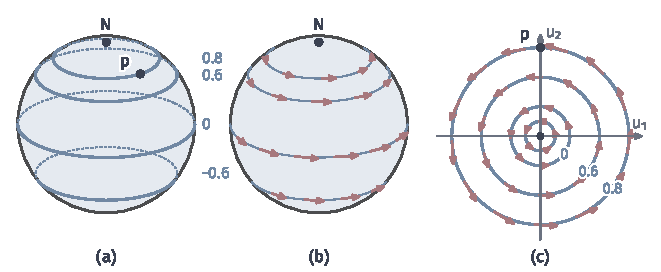
\includegraphics[width=112mm]{figures/04-spaces-measures-and-geometry/04-manifolds/matplotlib/mfd-height-rotation/figure.pdf}
  \caption{球面上的高度函数与旋转场。(a)蓝色纬线是$h=y_3$的等高线，右侧数字是高度，背面用虚线。(b)绕竖直轴的旋转场（红箭头）沿等高线切向，每点的箭头属于该点的切空间。(c)北极图中的同一组对象：半径$r$的圆对应高度$(r^2-1)/(r^2+1)$，半径$\tfrac12,1,2,3$的圆依次对应高度$-0.6,0,0.6,0.8$（最内圈未标数字），红箭头是分量$(-u_2,u_1)$的向量场，长度按比例缩小。}
  \label{fig:mfd-height-rotation}
\end{BookInlineFigure}

在北极，南极图坐标为$\bm w=\bm0$，$\tilde h$的偏导数在$\bm0$处都为零，所以$\mathrm dh_N=0$。这与极值的一般规律相符：若$f$在内点$p$处取局部最大值，则每条经过$p$的曲线$\gamma$使$f\circ\gamma$在$0$处取局部最大值，于是$\bm vf=(f\circ\gamma)'(0)=0$对所有$\bm v$成立，$\mathrm df_p=0$。球面紧，$h$的最大值一定取得，取在北极，微分在那里为零。

注意$\mathrm dh_p$是余切向量，不是一个“梯度方向”。要把它变成指向高度增加最快方向的切向量，需要在切空间上有内积，这一构造在第~\ref{chap:manifold-calculus}章完成。

\subsection{向量场与协向量场}
\label{sec:mfd-vector-covector-fields}

\paragraph{向量场}
设想球面绕竖直轴匀速旋转，每一点都有一个速度，它属于该点的切空间。把这些速度放在一起，就得到一个随点变化、每点取值在不同切空间中的对象，图~\ref{fig:mfd-height-rotation}(b)画的就是它。

\begin{definition}[光滑向量场]
\label{def:mfd-vector-field}
$M$上的\term{向量场}（vector field）$X$给每个$p\in M$指定一个切向量$X_p\in T_pM$。在坐标图$(U,\varphi)$中写成
\begin{equation}
X_p=\sum_{i=1}^nX_i(p)\,\partial_i|_p,\qquad p\in U,
\label{eq:mfd-vector-field-components}
\end{equation}
函数$X_i:U\to\mathbb R$称为$X$的分量。若在每张坐标图中分量都光滑，则称$X$为光滑向量场。$M$上全体光滑向量场的集合记为$\mathfrak X(M)$。
\end{definition}

两张图重叠处，分量按式~\eqref{eq:mfd-tangent-change}逐点变换：
\begin{equation}
\tilde X_k=\sum_{j=1}^n\frac{\partial\tilde x_k}{\partial x_j}\,X_j .
\label{eq:mfd-vector-field-change}
\end{equation}
转移映射的偏导数是光滑函数，所以一张图中分量光滑，另一张图中分量也光滑，只需在一个图册中检查。反过来，若在一个图册的每张图中给定一组光滑函数，并在每个重叠处满足式~\eqref{eq:mfd-vector-field-change}，它们就拼成一个光滑向量场。

\paragraph{协向量场}
同样地，给每点指定一个余切向量，就得到\term{协向量场}（covector field）$\omega$。在图中写成$\omega_p=\sum_ia_i(p)\,\mathrm dx_i|_p$，分量光滑时称为光滑协向量场，重叠处的系数按式~\eqref{eq:mfd-covector-change}变换。最重要的例子是光滑函数的微分：$\mathrm df$在图中的分量是$\partial\hat f/\partial x_i$，光滑，所以$\mathrm df$是光滑协向量场。

\paragraph{例子：球面的旋转场}
绕竖直轴转角$t$的旋转把$\bm y$送到
\[
(y_1\cos t-y_2\sin t,\ y_1\sin t+y_2\cos t,\ y_3),
\]
它不改变$y_3$。由式~\eqref{eq:mfd-stereographic-north}，北极图坐标$\bm u=(y_1,y_2)/(1-y_3)$随之做同一个平面旋转。对$t$在$0$处求导，旋转场在北极图中的分量为
\begin{equation}
(X_1,X_2)=(-u_2,\ u_1).
\label{eq:mfd-rotation-north}
\end{equation}
同理，在南极图中分量为$(-w_2,w_1)$，北极$\bm w=\bm0$处场值为零，这是绕轴旋转时轴上的点不动。

用式~\eqref{eq:mfd-vector-field-change}核对两组分量相容。由式~\eqref{eq:mfd-inversion-jacobian}，先注意$\bm u^\top(-u_2,u_1)^\top=0$，于是
\[
\bm J_\tau(\bm u)\begin{bmatrix}-u_2\\u_1\end{bmatrix}
=\frac{1}{\rho}\begin{bmatrix}-u_2\\u_1\end{bmatrix}.
\]
而$\bm w=\bm u/\rho$，右端恰是$(-w_2,w_1)$。两组分量拼成整个球面上的光滑向量场。

\paragraph{向量场作用于函数}
向量场与函数配合，逐点取方向导数，得到一个新函数：
\begin{equation}
(Xf)(p)=X_pf=\mathrm df_p(X_p).
\label{eq:mfd-field-on-function}
\end{equation}
在坐标图中，$Xf=\sum_iX_i\,\partial\hat f/\partial x_i$。$X$与$f$都光滑时，$Xf$光滑。映射$f\mapsto Xf$是线性的，并满足$X(fg)=f\,Xg+g\,Xf$。

例如旋转场作用于高度函数。由上一小节的偏导数，
\[
Xh=-u_2\cdot\frac{4u_1}{(\rho+1)^2}+u_1\cdot\frac{4u_2}{(\rho+1)^2}=0 .
\]
这符合直观：绕竖直轴旋转不改变高度。图~\ref{fig:mfd-height-rotation}(c)中红箭头沿等高线走，说的是同一件事。

\paragraph{场的逐点运算与不同点的比较}
同一点处的场值属于同一个切空间，所以$X+Y$、$gX$（$g$为光滑函数）可以逐点定义，结果仍是光滑向量场。不同点处的场值却属于不同的切空间，差$X_p-X_q$没有意义。用坐标分量相减看似可行，但结果依赖所选的图。

下面用一个具体计算说明这一点。在北极图中取常值分量的场$X=\partial_{u_1}$，定义在$S^2\setminus\{N\}$上。取$p=\sigma_N^{-1}(0,3)$与$q=\sigma_N^{-1}(1,0)=(1,0,0)$，北极图中两点处的分量都是$(1,0)$，相减为零，看起来是“同一个向量”。

换到南极图。由式~\eqref{eq:mfd-inversion-jacobian}，在$q$处$\bm J_\tau(1,0)=\operatorname{diag}(-1,1)$，于是两点处的分量分别是
\[
p:\ \bm J_\tau(0,3)(1,0)^\top=(\tfrac19,\ 0),\qquad
q:\ \bm J_\tau(1,0)(1,0)^\top=(-1,\ 0).
\]
两者之差不为零。可见“两个不同点处的切向量是否相同”没有与图无关的答案。比较不同点的方向需要额外的搬运规则，这是第~\ref{chap:riemannian-geometry}章联络与平行移动的任务。

\subsection{向量场的Lie括号}
\label{sec:mfd-lie-bracket}

向量场可以先后作用于函数。$Y$作用于$f$得到函数$Yf$，$X$再作用得到$X(Yf)$，交换次序得$Y(Xf)$。在欧氏空间中，常系数的偏导数可以交换次序；系数随点变化时，两种次序一般不同。这个差既不依赖度量，也有清楚的运动含义。

\paragraph{交换差仍是向量场}
两个一阶导数的复合本来是二阶算子，先写出来看。在坐标中记$X=\sum_iX_i\partial_i$，$Y=\sum_jY_j\partial_j$，$\hat f$为$f$的坐标表示，由乘积法则，
\[
X(Yf)=\sum_{i,j}X_i\,(\partial_iY_j)\,\partial_j\hat f+\sum_{i,j}X_iY_j\,\partial_i\partial_j\hat f .
\]
$Y(Xf)$的展开相同，只是$X,Y$对调。二阶偏导数可交换，两式中的二阶项相同，相减时抵消，只剩一阶项：
\begin{equation}
X(Yf)-Y(Xf)=\sum_{j=1}^n\Bigl(\sum_{i=1}^n\bigl(X_i\,\partial_iY_j-Y_i\,\partial_iX_j\bigr)\Bigr)\partial_j\hat f .
\label{eq:mfd-lie-bracket-coordinates}
\end{equation}
右端是某个向量场作用于$f$的结果，它的分量是括号中的光滑函数。

\begin{definition}[Lie括号]
\label{def:mfd-lie-bracket}
对$X,Y\in\mathfrak X(M)$，由
\begin{equation}
[X,Y]f=X(Yf)-Y(Xf)
\label{eq:mfd-lie-bracket-def}
\end{equation}
确定的向量场$[X,Y]$称为$X$与$Y$的\term{Lie括号}（Lie bracket）。在坐标图中，它的分量由式~\eqref{eq:mfd-lie-bracket-coordinates}给出。
\end{definition}

还要说明不同图中的分量拼成同一个向量场。在图$\varphi$中把式~\eqref{eq:mfd-lie-bracket-coordinates}定义的场记为$Z$，在图$\psi$中记为$\tilde Z$。二者在重叠处作用于任意光滑函数，都等于与图无关的$X(Yf)-Y(Xf)$。

把$f$取为第二张图的坐标函数$\tilde x_k$（只在重叠的开集上用，方向导数只依赖函数在点附近的值），得到
\[
\tilde Z_k=Z\tilde x_k=\sum_{j=1}^n Z_j\,\frac{\partial\tilde x_k}{\partial x_j},
\]
这正是变换规则\eqref{eq:mfd-vector-field-change}。

\paragraph{一个计算例子}
在$\mathbb R^2$上取$X=\partial_1$，$Y=x_1\partial_2$。由式~\eqref{eq:mfd-lie-bracket-coordinates}，$[X,Y]$的第二个分量是$X_1\partial_1Y_2=1$，其余为零，所以
\[
[X,Y]=\partial_2 .
\]
对函数直接核对。两种先后次序分别是
\[
X(Yf)=\partial_1(x_1\partial_2f)=\partial_2f+x_1\partial_1\partial_2f,\qquad
Y(Xf)=x_1\partial_2\partial_1f .
\]
相减得$\partial_2f$，与上面一致。

这个结果可以从运动的角度理解。沿$X$走时间$\varepsilon$是向右平移$\varepsilon$；沿$Y$走时间$\varepsilon$是把$(a,b)$变为$(a,b+\varepsilon a)$，向上移动的距离取决于当时的横坐标。从$(a,b)$出发，两种走法的终点分别是
\[
\text{先}X\text{后}Y:\ (a+\varepsilon,\ b+\varepsilon a+\varepsilon^2),\qquad
\text{先}Y\text{后}X:\ (a+\varepsilon,\ b+\varepsilon a).
\]
两条路线的终点相差$(0,\varepsilon^2)$，是二阶小量，方向正是$\partial_2$。Lie括号度量的就是两种运动先后次序不可交换的程度，图~\ref{fig:mfd-lie-bracket}画出了这两条路线。

\begin{BookInlineFigure}
  \centering
  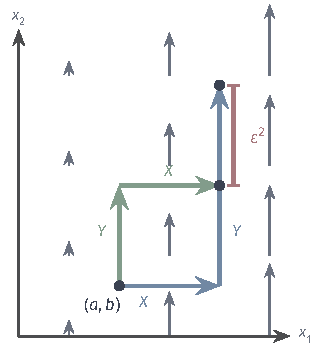
\includegraphics[width=54.906mm]{figures/04-spaces-measures-and-geometry/04-manifolds/tikz/mfd-lie-bracket/figure.pdf}
  \caption{Lie括号是运动次序的差。灰色箭头是场$Y=x_1\partial_2$，越往右越长。从$(a,b)=(1,\tfrac12)$出发，取$\varepsilon=1$：蓝色路线先沿$X=\partial_1$再沿$Y$，绿色路线先沿$Y$再沿$X$，终点相差红色线段$\varepsilon^2=1$，方向是$[X,Y]=\partial_2$。蓝色路线走$Y$时横坐标已经变大，所以走得更高。}
  \label{fig:mfd-lie-bracket}
\end{BookInlineFigure}

\paragraph{基本性质}
由定义直接可得反对称性与线性，对实数$a,b$和光滑函数$g$有
\[
\begin{gathered}
[X,Y]=-[Y,X],\qquad [aX+bY,Z]=a[X,Z]+b[Y,Z],\\
[X,gY]=g[X,Y]+(Xg)Y .
\end{gathered}
\]
此外还有Jacobi恒等式
\[
[X,[Y,Z]]+[Y,[Z,X]]+[Z,[X,Y]]=0,
\]
把三项都作用于$f$并按定义展开，得到十二个三阶复合项，它们两两抵消。坐标基向量场的Lie括号为零，$[\partial_i,\partial_j]=0$，这正是二阶偏导数可交换。

Lie括号的定义只用到向量场作用于函数，不需要先选度量或联络。第~\ref{chap:riemannian-geometry}章用它表述联络的无挠条件与曲率，第~\ref{chap:lie-groups}章用它刻画连续变换群在单位元附近的结构。

\section{光滑单位分解}
\label{sec:mfd-partition-unity}

很多构造在一张坐标图里很容易完成，例如在坐标中写下一个函数、一个向量场或一个内积。但整个流形通常需要多张图，各图上的构造在重叠处一般不一致，不能直接拼接。办法是给每张图配一个光滑权重，只在该图内部取正值，所有权重之和处处为一；各图上的构造乘以权重后相加，在每点附近只涉及有限项，结果就是整体上光滑的对象。本节构造这样的权重。

\paragraph{支撑受限的光滑函数}
第一步要有在一个区域外恒为零、在区域内为正的光滑函数。多项式做不到这一点：非零多项式不能在一个区间上恒为零。下面的函数在原点处以所有阶导数为零的方式“起飞”：
\begin{equation}
\eta(t)=\begin{cases}e^{-1/t},&t>0,\\0,&t\leq0.\end{cases}
\label{eq:mfd-smooth-step}
\end{equation}
当$t>0$时，$\eta$的$k$阶导数形如$P_k(1/t)e^{-1/t}$，$P_k$是多项式；令$s=1/t\to+\infty$，$P_k(s)e^{-s}\to0$，所以各阶导数从右侧趋于零，与左侧的零函数衔接，$\eta$在$\mathbb R$上光滑。

用$\eta$可以造出欧氏空间中的光滑截断函数。对$0<r<R$，令
\[
\chi(\bm x)=\frac{\eta(R^2-\lVert\bm x\rVert_2^2)}{\eta(R^2-\lVert\bm x\rVert_2^2)+\eta(\lVert\bm x\rVert_2^2-r^2)} .
\]
分母的两项不会同时为零，因为$\lVert\bm x\rVert_2^2<R^2$与$\lVert\bm x\rVert_2^2>r^2$至少有一个成立。于是$\chi$光滑，取值在$[0,1]$中，在半径$r$的闭球上恒为$1$，在半径$R$的球外恒为$0$。这类函数称为\term{截断函数}（cutoff function）。

函数$f$的\term{支撑}（support）是集合$\{p:f(p)\neq0\}$的闭包，记为$\operatorname{supp}f$。取闭包是为了让“$f$在支撑之外恒为零”成为开集上的性质：$\chi$的支撑是半径$R$的闭球。把$\chi$放进一张坐标图，并乘到坐标表示上，就能把局部构造截断成在整个流形上有定义的函数，前提是截断后的支撑落在图的定义域内部。

\paragraph{局部有限的覆盖}
多个权重相加时，若每点附近有无穷多个权重非零，和可能不收敛，也可能不光滑。所以需要覆盖满足局部有限条件。设$\{V_\beta\}$是$M$的一族子集，若每点都有一个邻域只与其中有限个$V_\beta$相交，则称这族子集\term{局部有限}（locally finite）。若一个开覆盖$\{V_\beta\}$的每个成员都含于给定开覆盖$\{U_\alpha\}$的某个成员中，则称前者是后者的一个\term{细化}（refinement）。

\begin{definition}[光滑单位分解]
\label{def:mfd-partition-unity}
设$\{U_\alpha\}_{\alpha\in A}$是$M$的开覆盖。一族光滑函数$\{\psi_\alpha\}_{\alpha\in A}$称为从属于$\{U_\alpha\}$的光滑\term{单位分解}（partition of unity），若：
\begin{enumerate}
\item 对每个$\alpha$，$0\leq\psi_\alpha\leq1$且$\operatorname{supp}\psi_\alpha\subseteq U_\alpha$；
\item 支撑族$\{\operatorname{supp}\psi_\alpha\}$局部有限；
\item 对每个$p\in M$，$\sum_{\alpha}\psi_\alpha(p)=1$。
\end{enumerate}
\end{definition}

由局部有限性，每点附近只有有限个$\psi_\alpha$不为零，所以第三条中的和在每点附近是有限和，自然光滑。

\paragraph{一维的例子}
在$\mathbb R$上取开覆盖$U_1=(-\infty,1)$、$U_2=(-1,\infty)$。令
\[
\psi_1(x)=\frac{\eta(\tfrac12-x)}{\eta(\tfrac12-x)+\eta(x+\tfrac12)},\qquad
\psi_2(x)=\frac{\eta(x+\tfrac12)}{\eta(\tfrac12-x)+\eta(x+\tfrac12)} .
\]
对每个$x$，$x<\tfrac12$与$x>-\tfrac12$至少有一个成立，分母为正。两函数都光滑，取值于$[0,1]$，和为$1$。$\psi_1$的支撑是$(-\infty,\tfrac12]$，含于$U_1$；$\psi_2$的支撑是$[-\tfrac12,\infty)$，含于$U_2$。

这里特意把截断点取在$\pm\tfrac12$而不是$\pm1$。若用$\eta(1-x)$，支撑就是$(-\infty,1]$，不含于开集$U_1$。支撑必须严格落在开集内，乘上权重的局部构造才能在开集的边缘以外光滑地补零。

\paragraph{存在定理}
单位分解的存在要用到流形定义中的全部条件：局部欧氏性提供坐标球上的截断函数，Hausdorff性与第二可数性保证能把覆盖细化为局部有限的。

\begin{theorem}[光滑单位分解的存在]
\label{thm:mfd-partition-unity-existence}
设$M$是光滑流形，可以带边界，$\{U_\alpha\}_{\alpha\in A}$是$M$的任一开覆盖。则存在从属于$\{U_\alpha\}$的光滑单位分解。
\end{theorem}

\begin{proof}
先处理$M$紧的情形，它已包含构造的全部想法。对每个$p\in M$，取包含$p$的坐标图$(V,\varphi)$与某个$U_\alpha\ni p$，在$\varphi(V\cap U_\alpha)$中取以$\varphi(p)$为中心、半径为$R_p$的球，其闭包仍在其中。令$B_p$为半径$R_p/2$的同心球在$\varphi^{-1}$下的原像。边界点处用半球代替球，下同。

$\{B_p\}$覆盖$M$，由紧性可选出有限个$B_{p_1},\ldots,B_{p_m}$覆盖$M$。对每个$k$，取截断函数$\chi_k$，在半径$R_{p_k}/2$的闭球上为$1$，在半径$\tfrac34R_{p_k}$的球外为$0$。令$\lambda_k=\chi_k\circ\varphi_k$在图内，图外为$0$。$\lambda_k$的支撑是半径$\tfrac34R_{p_k}$的闭球的原像，它是紧集，在Hausdorff空间中是闭集，所以图外补零后$\lambda_k$在$M$上光滑。

$\lambda_k\geq0$，并在$B_{p_k}$上等于$1$，所以$\Lambda=\sum_k\lambda_k$处处至少为$1$。令$\tilde\psi_k=\lambda_k/\Lambda$，它们光滑、非负、和为一，且每个$\tilde\psi_k$的支撑含于某个$U_{\alpha(k)}$。最后对每个$\alpha$令$\psi_\alpha=\sum_{k:\alpha(k)=\alpha}\tilde\psi_k$，空和取$0$，就得到以原指标集编号的单位分解。

一般情形只需把“选有限个$B_p$”换成“选局部有限的可数个”。第二可数性与局部欧氏性给出一列紧集$K_1\subseteq K_2\subseteq\cdots$，满足$K_j$含于$K_{j+1}$的内部且$\bigcup_jK_j=M$。对每个$j$，紧集$K_{j+1}\setminus\operatorname{int}K_j$可用有限个如上的坐标球覆盖，并让这些球含于$\operatorname{int}K_{j+2}\setminus K_{j-1}$。每点只与相邻几层的球相交，所以全部球组成局部有限的覆盖，其余步骤与紧情形相同。紧集列的构造这里不展开，它是第二可数局部紧Hausdorff空间的一般性质。
\end{proof}

\paragraph{单位分解的用途}
单位分解的典型用法是“局部构造，加权求和”。设$f_\alpha$是定义在$U_\alpha$上的光滑函数，则$\sum_\alpha\psi_\alpha f_\alpha$在整个$M$上有定义并且光滑，其中每项在$U_\alpha$外按零理解。若所有$f_\alpha$在某点附近都等于同一个值，加权和在那里也等于这个值，因为权重之和为一。

由此可得两个直接结论。第一，任一点$p$的任一邻域中都有光滑函数在$p$附近等于某个给定的局部光滑函数，在邻域外为零；这说明局部定义的坐标函数可以截断成全局光滑函数，切向量完全由它对全局光滑函数的作用确定。第二，在每张图中取欧氏内积，用单位分解加权相加，就在每个切空间上得到一个内积。正定性在加权求和下保持，因为每点处的权重非负、和为一，至少有一项严格为正。这正是第~\ref{chap:riemannian-geometry}章黎曼度量存在的依据。同样的手法也用于把局部坐标中的积分拼成流形上的积分，见第~\ref{chap:manifold-calculus}章。

\section{本章小结}
\label{sec:mfd-summary}

本章开头的问题是：经纬度在两极失效、角度绕圆一周会跳跃，这样的对象应当怎样记录？回答是放弃单张全局坐标，改用一族局部坐标图，并要求重叠处的转移映射光滑可逆。圆周的转移映射是平移，球极投影的转移映射是反演$\bm u/\lVert\bm u\rVert_2^2$，环面的转移映射是圆周转移映射的并排。

流形因此是一个整体空间：Hausdorff且第二可数，每点附近同胚于欧氏开集。光滑结构由光滑相容的坐标图决定，同一拓扑空间上可以有不同的光滑结构，例如$\mathbb R$上$x\mapsto x^3$给出的图与恒等图不相容。允许局部模型为半空间，就得到带边界流形；边界点的身份与图无关，边界本身是低一维的无边界流形，带角点的集合不属于这种光滑边界情形。

局部欧氏结构使流形的整体拓扑比一般拓扑空间规整。坐标球路径连通，所以路径分支都是既开又闭的，连通与路径连通等价；第二可数性又使连通分支至多可数。紧流形可以用有限张图覆盖，但正维数的紧无边界流形不能只用一张图，球面上的经纬度困难正源于此。

本章区分了三个层次的对象，表~\ref{tab:mfd-summary-records}用球面上的点$p=(0,\tfrac35,\tfrac45)$把它们并排列出。点是空间的元素，坐标的加法依赖图，不是点的运算。切向量是曲线速度的等价类，分量按转移映射的Jacobian矩阵变换；边界点处切空间用坐标记录定义，单侧可行的方向只占其中的半空间。余切向量是切向量的线性读数，系数按Jacobian矩阵的逆转置变换，在选定度量之前不能与切向量等同。

\begin{BookInlineTable}
  \centering
  \begin{tabular}{llll}
    \toprule
    对象 & 北极图 & 南极图 & 换算\\
    \midrule
    点$p$ & $(0,3)$ & $(0,\tfrac13)$ & $\tau$\\
    切向量$\partial_{u_1}|_p$ & $(1,0)$ & $(\tfrac19,0)$ & $\bm J$\\
    余切向量$\mathrm dh_p$ & $(0,0.12)$ & $(0,-1.08)$ & $\bm J^{-\top}$\\
    \bottomrule
  \end{tabular}
  \caption{球面上同一组对象在两张图中的记录，其中$\bm J=\operatorname{diag}(\tfrac19,-\tfrac19)$。}
  \label{tab:mfd-summary-records}
\end{BookInlineTable}

随点变化的对象在坐标中由分量记录，分量光滑即对象光滑。光滑函数的微分$\mathrm df_p$是余切向量，内点处的局部极值点微分为零。向量场作用于函数得到方向导数，两个向量场先后作用的交换差是一阶算子，给出Lie括号，它不依赖度量或联络。同一点的场值可以运算，不同点处的场值属于不同的切空间，坐标分量之差依赖图，不能当作它们的比较。光滑单位分解把各图上的构造加权拼成整体，依赖流形定义中的全部条件。

这些都是单个流形内部的结构。点从一个流形映到另一个流形时，切向量与余切向量怎样随之改变，是第~\ref{chap:manifold-maps}章的问题；比较不同点处的方向、度量长度和距离，要在第~\ref{chap:riemannian-geometry}章引入黎曼度量与联络。


\chapter{流形上的映射}
\label{chap:manifold-maps}

把地球仪绕地轴转过一个角度，每个城市都移到了新的位置；在球面上画一条航线，就是把时间区间映到球面上。这两件事都是流形之间的映射。映射首先对应点：给定原来的点，找到它被送到哪里。但我们还关心更多：经过一点的运动方向被转到哪个方向，速度是否被拉伸，一个方向上的读数怎样随映射换算。这些问题的答案不在点的对应本身，而在映射的微分中。

本章沿“点—方向—读数”的顺序展开。第~\ref{sec:mmaps-smooth-maps}节用两侧的坐标图定义流形之间的光滑映射，区分同一点的坐标改写与把点实际移到另一点，并把第~\ref{chap:manifold-basics}章的曲线和函数看作特例。第~\ref{sec:mmaps-differentials}节由曲线速度的推送得到切空间之间的线性映射，再考察对整个向量场逐点推送时会遇到的困难：一般映射的推送结果未必在目标上构成向量场。

第~\ref{sec:mmaps-pullback}节转向余切向量。读数的换算方向与切向量相反，从目标点拉回到原像点；正因为方向相反，协向量场的拉回对任何光滑映射都有定义，不受推送向量场时遇到的限制。拉回与函数微分的关系$\mathrm d(f\circ F)=F^*(\mathrm df)$把两个方向的运算联系起来。

本章只处理给定映射的局部操作。用映射判断两个流形是否在光滑意义下等价、一个流形能否作为另一个流形的子流形，需要整体的可逆性与拓扑条件，这是第~\ref{chap:manifold-relations}章的任务；一般微分形式的拉回在第~\ref{chap:manifold-calculus}章定义交替形式之后推广。

\section{光滑映射}
\label{sec:mmaps-smooth-maps}

设$M$是$m$维光滑流形，$N$是$n$维光滑流形，$F:M\to N$是映射。判断$F$是否光滑，仍要借助坐标，但现在两侧都要用图：输入的点用$M$的图记录，输出的点用$N$的图记录。这样得到的是欧氏开集之间的映射，可以用多元微积分检查。

\paragraph{坐标表示与光滑性}
设$(U,\varphi)$是$M$的图，$(V,\psi)$是$N$的图，并且$F(U)\subseteq V$。把输入坐标先送回点，作用$F$，再读出输出坐标，得到
\begin{equation}
\hat F=\psi\circ F\circ\varphi^{-1}:\varphi(U)\to\psi(V)\subseteq\mathbb R^n ,
\label{eq:mmaps-coordinate-representation}
\end{equation}
称为$F$在这对图下的\term{坐标表示}（coordinate representation）。条件$F(U)\subseteq V$保证输出点能用同一张图$\psi$读出。

\begin{definition}[光滑映射]
\label{def:mmaps-smooth-map}
映射$F:M\to N$称为\term{光滑映射}（smooth map），若$F$连续，并且对每个$p\in M$，存在包含$p$的图$(U,\varphi)$与包含$F(p)$的图$(V,\psi)$，使$F(U)\subseteq V$且坐标表示\eqref{eq:mmaps-coordinate-representation}光滑。$M$或$N$带边界时，光滑性按第~\ref{chap:manifold-basics}章的约定理解：半空间开子集上的映射光滑，指它在每点附近能光滑延拓到一个欧氏开邻域上。
\end{definition}

连续性的作用是保证满足$F(U)\subseteq V$的图存在：任给包含$F(p)$的图$(V,\psi)$，$F^{-1}(V)$是包含$p$的开集，把$M$的图限制到$U\cap F^{-1}(V)$上即可。

\paragraph{与图的选择无关}
定义只要求每点附近存在一对图使坐标表示光滑。换用别的图对，结论不变：若$(U',\varphi')$与$(V',\psi')$是另一对满足条件的图，在重叠处
\[
\psi'\circ F\circ\varphi'^{-1}=(\psi'\circ\psi^{-1})\circ\hat F\circ(\varphi\circ\varphi'^{-1}),
\]
右端是两个光滑坐标变换与$\hat F$的复合，仍光滑。同样的论证说明光滑映射的复合仍是光滑映射：若$F:M\to N$与$G:N\to P$都光滑，则在合适的图下$\widehat{G\circ F}=\hat G\circ\hat F$，光滑映射的复合光滑。

\paragraph{特例：曲线与函数}
第~\ref{chap:manifold-basics}章的两类对象都是光滑映射的特例。把区间$I$看作一维流形（带端点时为带边界流形），用恒等映射作图，光滑曲线$\gamma:I\to M$就是$I$到$M$的光滑映射，坐标表示是坐标曲线$\varphi\circ\gamma$。把$\mathbb R$看作一维流形，光滑函数$f:M\to\mathbb R$就是$M$到$\mathbb R$的光滑映射，坐标表示是$\hat f=f\circ\varphi^{-1}$。今后关于一般光滑映射的结论，都可以用这两类特例检验。

\paragraph{例子：球面的旋转}
设$\bm R(\theta)$是平面上转角为$\theta$的旋转矩阵。绕竖直轴转$\theta$的映射
\[
R_\theta:S^2\to S^2,\qquad R_\theta(\bm y)=(\bm R(\theta)(y_1,y_2)^\top,\;y_3)
\]
把球面送到自身。在北极图中，$\sigma_N(R_\theta(\bm y))=\bm R(\theta)(y_1,y_2)^\top/(1-y_3)=\bm R(\theta)\sigma_N(\bm y)$，所以坐标表示是线性映射$\hat R_\theta(\bm u)=\bm R(\theta)\bm u$，光滑。北极是$R_\theta$的不动点，那里改用南极图，坐标表示同样是$\bm w\mapsto\bm R(\theta)\bm w$。于是$R_\theta$是光滑映射。

绕水平轴的旋转会把北极移走，这时需要按点选择图。例如绕$y_1$轴转$\pi/2$的映射$Q(\bm y)=(y_1,-y_3,y_2)$把北极送到$(0,-1,0)$，把点$(0,1,0)$送到北极。在$(0,1,0)$附近，输入可以用北极图，输出却必须用南极图，因为北极不在北极图的定义域内。定义中“对每个$p$存在一对图”正是为这种情况准备的。

\paragraph{改写坐标与移动点}
同一个计算式可以表示两件不同的事。取$p=(0,\tfrac35,\tfrac45)$，北极图坐标为$(0,3)$。旋转$R_\theta$把$p$送到$(-\tfrac35\sin\theta,\tfrac35\cos\theta,\tfrac45)$，坐标变为$(-3\sin\theta,3\cos\theta)$：点真的移动了，坐标的变化反映了这一移动。坐标变换$\tau=\sigma_S\circ\sigma_N^{-1}$把$(0,3)$变为$(0,\tfrac13)$，点却没有动，只是换了一张图来记录。

用本节的语言说，坐标变换是恒等映射$\mathrm{id}:S^2\to S^2$在输入用$\sigma_N$、输出用$\sigma_S$时的坐标表示。所以判断一个坐标公式描述的是什么，不能只看公式，还要看它是同一映射在不同图下的表示，还是不同映射在同一图下的表示。前者改变的是记录，后者改变的是点；后文讨论微分时，前者只改变切向量的分量，后者把切向量送到另一个点的切空间。

\section{映射的微分}
\label{sec:mmaps-differentials}

点被映射移动时，经过它的运动也跟着改变。地球仪转过一个角度，沿一条经线向北的航线被转到另一条经线上，航线上每点的运动方向也都被带到了别处。本节先对单个切向量回答“方向被送到哪里”，得到切空间之间的线性映射；再对整个向量场逐点执行这一操作，看结果能否在目标流形上构成向量场。

前者对任何光滑映射都成立，后者却需要映射满足额外条件。两者的差别，就是下一节拉回运算的出发点。

\subsection{切向量的推送}
\label{sec:mmaps-tangent-pushforward}

\paragraph{由曲线速度定义}
先回忆欧氏空间的情形。映射$\bm f:\mathbb R^m\to\mathbb R^n$在$\bm x$处的Jacobian矩阵$\bm J$是最佳线性近似：小位移$\bm h$引起的输出变化约为$\bm J\bm h$，详见\BookChapterRef{chap:multivariate-differentiation}{卷二第17章“多元函数微分”}。流形上不能写$p+\bm h$，因为点不能相加，所以要把“小位移”换成“经过$p$的曲线及其速度”。

先在坐标里看这个近似长什么样。对投影的坐标表示\eqref{eq:mmaps-projection-chart}求偏导，第$i$个分量对$u_j$求导，由商的求导法则得到
\[
\frac{\partial\hat\pi_i}{\partial u_j}
=\frac{2\delta_{i,j}}{\rho+1}-\frac{4u_iu_j}{(\rho+1)^2}.
\]
写成矩阵，
\begin{equation}
\bm J_{\hat\pi}(\bm u)=\frac{2}{\rho+1}\bm I-\frac{4}{(\rho+1)^2}\bm u\bm u^\top .
\label{eq:mmaps-projection-jacobian}
\end{equation}

在$\bm u=(0,3)$处，$\rho=9$，$\bm u\bm u^\top=\operatorname{diag}(0,9)$，代入后
\[
\bm J_{\hat\pi}(0,3)=\frac15\bm I-\frac{1}{25}\operatorname{diag}(0,9)
=\operatorname{diag}(0.2,\ -0.16).
\]
验证近似的精度。把$u_2$从$3$改为$3.2$，由式~\eqref{eq:mmaps-projection-chart}，投影的第二个分量从$0.6$变为$6.4/11.24\approx0.5694$，变化量约为$-0.0306$。线性近似给出
\[
-0.16\times0.2=-0.032,
\]
两者只差$0.0014$。

图~\ref{fig:mmaps-linear-approx}把这种近似画成方格的形变：方格越小，弯曲的像越接近平行四边形。微分要提取的就是这个平行四边形所代表的线性映射。

\begin{BookInlineFigure}
  \centering
  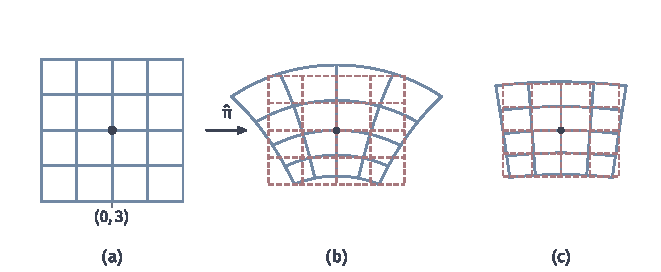
\includegraphics[width=112mm]{figures/04-spaces-measures-and-geometry/04-manifolds/matplotlib/mmaps-linear-approx/figure.pdf}
  \caption{微分是局部线性近似。(a)北极图中以$(0,3)$为心、半边长$0.8$的方格。(b)方格在$\hat\pi$下的像（蓝）与线性映射$\bm J=\operatorname{diag}(0.2,-0.16)$的像（红虚线），二者都按比例放大并平移到同一中心。(c)半边长缩小到$0.2$再放大相应倍数，蓝红两组线几乎重合。}
  \label{fig:mmaps-linear-approx}
\end{BookInlineFigure}

现在在流形上做同样的事。设$F:M\to N$光滑，$p$是内点，$\gamma$是经过$p$的曲线，$\gamma(0)=p$。$F$把它送成经过$F(p)$的曲线$F\circ\gamma$。取一对图，并记$\bm J_{\hat F}$为坐标表示的Jacobian矩阵。由欧氏链式法则，
\begin{equation}
(\psi\circ F\circ\gamma)'(0)=\bm J_{\hat F}(\varphi(p))\,(\varphi\circ\gamma)'(0).
\label{eq:mmaps-velocity-push}
\end{equation}

这个式子说了两件事。右端只依赖$\gamma$在$p$处的坐标速度，所以等价的两条曲线被送成等价的曲线，“把曲线送过去再取速度”是定义在$T_pM$上的操作。右端又是矩阵乘向量，所以这个操作是线性的。图~\ref{fig:mmaps-pushforward-sphere}（见本小节末的例子）是它在球面上的样子。

\begin{definition}[映射的微分]
\label{def:mmaps-differential}
设$F:M\to N$光滑，$p\in M$，$(U,\varphi)$与$(V,\psi)$是定义~\ref{def:mmaps-smooth-map}中的一对图。$F$在$p$处的\term{微分}（differential）是线性映射
\begin{equation}
\mathrm dF_p:T_pM\to T_{F(p)}N,
\label{eq:mmaps-differential}
\end{equation}
它把$p$处在图$\varphi$中分量为$\bm v$的切向量，送到$F(p)$处在图$\psi$中分量为$\bm J_{\hat F}(\varphi(p))\bm v$的切向量。切向量$\mathrm dF_p(\bm v)$称为$\bm v$在$F$下的\term{推送}（pushforward）。
\end{definition}

当$p$与$F(p)$都是内点时，式~\eqref{eq:mmaps-velocity-push}说明定义等价于
\[
\mathrm dF_p([\gamma])=[F\circ\gamma].
\]
这是最直观的理解：把曲线送过去，再取它的切向量。

在坐标基下，定义可以写成
\begin{equation}
\mathrm dF_p\Bigl(\left.\frac{\partial}{\partial x_j}\right|_p\Bigr)
=\sum_{k=1}^n\frac{\partial\hat F_k}{\partial x_j}(\varphi(p))
\left.\frac{\partial}{\partial y_k}\right|_{F(p)},
\label{eq:mmaps-differential-basis}
\end{equation}
其中$y_1,\ldots,y_n$是图$\psi$中的坐标。也就是说，$\mathrm dF_p$在两组坐标基下的矩阵就是坐标表示的Jacobian矩阵，第$j$列记录第$j$个输入基向量被送到哪里。

\paragraph{与图无关}
定义用了一对图，需要检查换图后得到的是同一个线性映射。换用另一对图$(U',\varphi')$与$(V',\psi')$，记坐标变换为$\tau_M=\varphi'\circ\varphi^{-1}$和$\tau_N=\psi'\circ\psi^{-1}$。坐标表示变成
\[
\hat F'=\tau_N\circ\hat F\circ\tau_M^{-1}.
\]

对它用链式法则，各处的Jacobian矩阵取在相应的点上，得到
\begin{equation}
\bm J_{\hat F'}=\bm J_{\tau_N}\,\bm J_{\hat F}\,\bm J_{\tau_M}^{-1}.
\label{eq:mmaps-jacobian-change}
\end{equation}

现在核对两种算法。同一切向量在新图中的分量是$\bm v'=\bm J_{\tau_M}\bm v$，代入式~\eqref{eq:mmaps-jacobian-change}，
\[
\bm J_{\hat F'}\bm v'=\bm J_{\tau_N}\bm J_{\hat F}\bm J_{\tau_M}^{-1}\bm J_{\tau_M}\bm v=\bm J_{\tau_N}(\bm J_{\hat F}\bm v).
\]
左端是用新图算出的输出分量，右端是旧图算出的输出向量换到新图后的分量，两者相等。所以微分是同一个线性映射，改变的只是它的矩阵，这与卷二中线性映射换基时矩阵的变化完全类似。

用旋转$R_{\pi/2}$核对一次。第~\ref{chap:manifold-basics}章给出转移映射$\tau$的Jacobian矩阵
\[
\bm J_\tau(\bm u)=\frac{\rho\bm I-2\bm u\bm u^\top}{\rho^2}.
\]
在$p$处，$\bm u=(0,3)$；在$R_{\pi/2}(p)$处，$\bm u=(-3,0)$。两处$\rho=9$，代入得
\[
\bm J_\tau(0,3)=\operatorname{diag}(\tfrac19,-\tfrac19),\qquad
\bm J_\tau(-3,0)=\operatorname{diag}(-\tfrac19,\tfrac19).
\]

北极图中旋转的矩阵是$\bm R(\tfrac\pi2)$。按式~\eqref{eq:mmaps-jacobian-change}换到南极图，先算右边两个因子，再乘左边的因子：
\[
\bm R(\tfrac\pi2)\operatorname{diag}(9,-9)
=\begin{bmatrix}0&9\\9&0\end{bmatrix},\qquad
\operatorname{diag}(-\tfrac19,\tfrac19)\begin{bmatrix}0&9\\9&0\end{bmatrix}
=\begin{bmatrix}0&-1\\1&0\end{bmatrix}.
\]
结果还是$\bm R(\tfrac\pi2)$，与第~\ref{sec:mmaps-smooth-maps}节在南极图中得到的坐标表示$\bm w\mapsto\bm R(\theta)\bm w$一致。

\paragraph{边界点处的微分}
边界点处，定义里的$\bm J_{\hat F}$要取坐标表示的光滑延拓的Jacobian矩阵。延拓不唯一，需要说明结果不受影响。设$\bm x$是半空间$\mathbb H^m$的边界点，$E_1,E_2$是$\hat F$在$\bm x$附近的两个光滑延拓。

关键在于，$\bm x$处的偏导数只用得到半空间内的函数值。沿边界方向$\bm e_j$（$j<m$）的差商，用到的点$\bm x+h\bm e_j$仍在边界上。沿内法方向$\bm e_m$，极限存在，所以可以只取$h>0$，用到的点$\bm x+h\bm e_m$在半空间内。这些点上$E_1=E_2=\hat F$，所以两个延拓的偏导数相同。

图~\ref{fig:mmaps-boundary-extension}是一维的情形：$[0,\infty)$上的函数$\sin x$有无穷多种光滑延拓，它们在$x<0$的部分可以相差很大，但在$x=0$处的斜率都是右导数$1$。

\begin{BookInlineFigure}
  \centering
  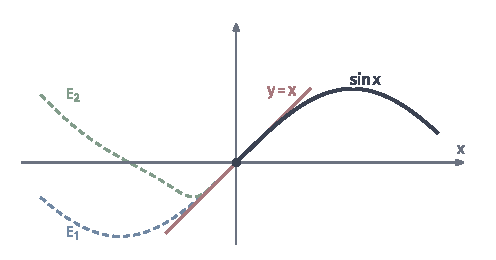
\includegraphics[width=84mm]{figures/04-spaces-measures-and-geometry/04-manifolds/matplotlib/mmaps-boundary-extension/figure.pdf}
  \caption{边界点处的微分与延拓无关。实线是定义在$[0,\infty)$上的$\sin x$；虚线是它在$x<0$处的两个光滑延拓$E_1=\sin x$与$E_2=\sin x+1.6\,e^{-1/x^2}$（$x<0$）。红线是二者在$0$处共同的切线$y=x$。}
  \label{fig:mmaps-boundary-extension}
\end{BookInlineFigure}

\paragraph{链式法则}
复合映射的微分是各步微分的复合。这是欧氏链式法则在流形上的形式，也是流形上做微分计算最常用的工具。

\begin{theorem}[链式法则]
\label{thm:mmaps-chain-rule}
设$F:M\to N$与$G:N\to P$都光滑，$p\in M$。则
\begin{equation}
\mathrm d(G\circ F)_p=\mathrm dG_{F(p)}\circ\mathrm dF_p .
\label{eq:mmaps-chain-rule}
\end{equation}
特别地，$\mathrm d(\mathrm{id}_M)_p$是$T_pM$上的恒等映射。
\end{theorem}

\begin{proof}
按定理~\ref{thm:mmaps-composition}的证明选取三张图，使$F$的输出图与$G$的输入图是同一张$\psi$，这时
\[
\widehat{G\circ F}=\hat G\circ\hat F .
\]
记$\bm x=\varphi(p)$。欧氏链式法则给出
\[
\bm J_{\hat G\circ\hat F}(\bm x)=\bm J_{\hat G}(\hat F(\bm x))\,\bm J_{\hat F}(\bm x).
\]
右端正是$\mathrm dG_{F(p)}$与$\mathrm dF_p$的矩阵之积。边界点处把各坐标表示换成光滑延拓，等式不变。

恒等映射在同一张图下的坐标表示是恒等映射，Jacobian矩阵为单位矩阵，第二个结论随之成立。
\end{proof}

\paragraph{秩}
$\mathrm dF_p$是有限维线性空间之间的线性映射，它有秩。秩说明映射在一点附近保留了多少个独立方向。

\begin{definition}[映射的秩]
\label{def:mmaps-rank}
线性映射$\mathrm dF_p$的秩称为$F$在$p$处的秩，记作$\operatorname{rank}_pF$。在坐标中，它等于$\bm J_{\hat F}(\varphi(p))$的秩。
\end{definition}

由式~\eqref{eq:mmaps-jacobian-change}，换图时矩阵左乘、右乘可逆矩阵，秩不变，所以这个定义与图无关。把它算出来，就知道映射在这一点把多少个方向“压扁”了。

投影$\pi$是最好的例子。式~\eqref{eq:mmaps-projection-jacobian}中，$\bm u\bm u^\top$只在方向$\bm u$上起作用，所以矩阵有两个特征方向。沿$\bm u$的特征值是
\[
\frac{2}{\rho+1}-\frac{4\rho}{(\rho+1)^2}=\frac{2(1-\rho)}{(\rho+1)^2},
\]
与$\bm u$垂直的方向上特征值是$2/(\rho+1)$。

后者永远不为零，前者只在$\rho=1$时为零。$\rho=1$的点正是赤道，因为这时$y_3=(\rho-1)/(\rho+1)=0$。于是$\pi$在赤道上秩为$1$，在其余点秩为$2$；北极不在这张图中，在南极图的原点用同样的公式得到矩阵$2\bm I$，秩也是$2$。

几何上这很合理，图~\ref{fig:mmaps-rank-projection}(a)(b)画出了这件事。赤道上切平面是竖直的，向下投影时其中的竖直方向被压成零，切平面只剩一条线；其余点的切平面只是被斜着压扁，仍然保持二维。

\begin{BookInlineFigure}
  \centering
  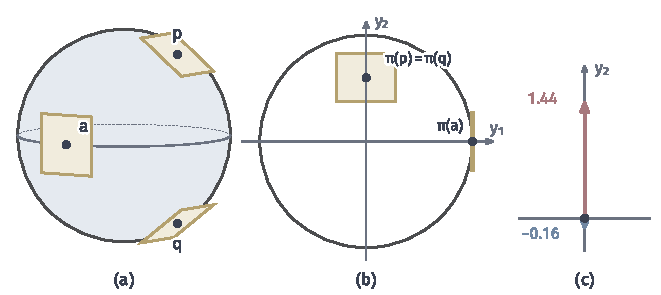
\includegraphics[width=112mm]{figures/04-spaces-measures-and-geometry/04-manifolds/matplotlib/mmaps-rank-projection/figure.pdf}
  \caption{投影$\pi$的秩与多个原像。(a)球面上的三小块切平面（黄），分别在$p=(0,\tfrac35,\tfrac45)$、$q=(0,\tfrac35,-\tfrac45)$与赤道点$a=(1,0,0)$处。(b)$p,q$处的切平面块投影成同一个矩形，秩为$2$；$a$处的切平面块投影成一条线段，秩为$1$。(c)$\partial_{u_2}$在$p$、$q$处的推送都在$\pi(p)$处的切空间中，第二分量分别为$-0.16$（蓝）与$1.44$（红）。}
  \label{fig:mmaps-rank-projection}
\end{BookInlineFigure}

高度函数$h$也可以这样看。它在两极以外秩为$1$，在两极秩为$0$，因为第~\ref{chap:manifold-basics}章已经算出$\mathrm dh_N=0$。可见秩会随点变化，只看一点的秩不能决定映射附近的形状，这个问题在第~\ref{chap:manifold-relations}章展开。

\paragraph{函数与曲线的情形}
第~\ref{chap:manifold-basics}章分别定义过函数的微分和曲线的速度，它们都应当是映射微分的特例，这里核对一下记号确实不冲突。

对光滑函数$f:M\to\mathbb R$，目标在每点$c$处的切空间由一个基向量$\frac{\mathrm d}{\mathrm dt}\big|_c$张成，把$a\,\frac{\mathrm d}{\mathrm dt}\big|_c$等同于实数$a$，就有$T_c\mathbb R=\mathbb R$。在这一等同下，式~\eqref{eq:mmaps-differential-basis}说明
\[
\mathrm df_p(\bm v)=\sum_{j=1}^m\frac{\partial\hat f}{\partial x_j}(\varphi(p))\,v_j ,
\]
这正是第~\ref{chap:manifold-basics}章定义的余切向量$\mathrm df_p$对切向量的读数。

对光滑曲线$\gamma:I\to M$，曲线的速度就是参数区间上单位切向量的推送：
\[
\gamma'(t_0)=\mathrm d\gamma_{t_0}\Bigl(\left.\frac{\mathrm d}{\mathrm dt}\right|_{t_0}\Bigr).
\]
于是链式法则\eqref{eq:mmaps-chain-rule}用到$F\circ\gamma$上，就得到前面“把曲线送过去再取速度”的公式：
\[
(F\circ\gamma)'(t_0)=\mathrm dF_{\gamma(t_0)}(\gamma'(t_0)).
\]

\paragraph{例子：旋转与高度函数}
旋转$R_\theta$在北极图中的坐标表示是线性映射$\bm R(\theta)$，线性映射的Jacobian矩阵就是它自己，所以微分在坐标基下的矩阵也是$\bm R(\theta)$。取$p=(0,\tfrac35,\tfrac45)$，把$\bm e_1$代入，得到
\[
\mathrm d(R_\theta)_p\bigl(\partial_{u_1}|_p\bigr)
=\cos\theta\,\partial_{u_1}|_{R_\theta(p)}+\sin\theta\,\partial_{u_2}|_{R_\theta(p)} .
\]
输入向量属于$T_pS^2$，输出向量属于$T_{R_\theta(p)}S^2$，是另一个点的切空间。$\bm R(\theta)$可逆，所以$R_\theta$在每点的秩都是$2$。

取$\theta=\pi/2$，上式变成
\[
\mathrm d(R_{\pi/2})_p(\partial_{u_1}|_p)=\partial_{u_2}|_{R_{\pi/2}(p)} .
\]
在$\mathbb R^3$中看一下这个结果是否合理。第~\ref{chap:manifold-basics}章算出$\partial_{u_1}|_p$的样子是$(\tfrac15,0,0)$，绕竖直轴转$\pi/2$后变成$(0,\tfrac15,0)$。

另一方面，对$\sigma_N^{-1}$关于$u_2$在$(-3,0)$处求导，第二个分量的导数是
\[
\frac{2(\rho+1)-4u_2^2}{(\rho+1)^2}=\frac{20}{100}=\frac15,
\]
其余两个分量含因子$u_2$，导数为零。所以$\partial_{u_2}|_{R_{\pi/2}(p)}=(0,\tfrac15,0)$，两边一致。图~\ref{fig:mmaps-pushforward-sphere}画的就是这组数据。

\begin{BookInlineFigure}
  \centering
  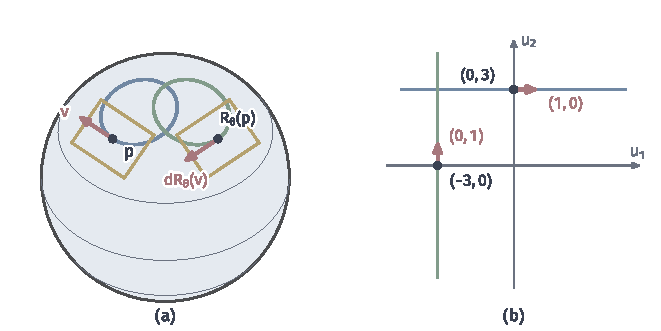
\includegraphics[width=112mm]{figures/04-spaces-measures-and-geometry/04-manifolds/matplotlib/mmaps-pushforward-sphere/figure.pdf}
  \caption{切向量的推送。(a)球面上，经过$p$的蓝色曲线$\gamma(t)=\sigma_N^{-1}(t,3)$被$R_\theta$（$\theta=\pi/2$）转成经过$R_\theta(p)$的绿色曲线，黄色平行四边形是两点处的切平面，红箭头是速度$\bm v=\partial_{u_1}|_p$及其推送，长度按实际放大$2$倍。(b)北极图中，两条曲线分别是直线$u_2=3$与$u_1=-3$，速度分量从$(1,0)$变为$(0,1)$。}
  \label{fig:mmaps-pushforward-sphere}
\end{BookInlineFigure}

旋转$Q$可以检验换图的情形。对式~\eqref{eq:mmaps-horizontal-rotation}在$\bm u=(0,1)$处求偏导。记分母为$D=\rho+1+2u_2$，此处$D=4$，$\partial_{u_1}D=0$，$\partial_{u_2}D=4$，第二个分子$1-\rho$在此处为零，于是
\[
\bm J_{\hat Q}(0,1)=\begin{bmatrix}2/D&0\\0&-2u_2/D\end{bmatrix}
=\operatorname{diag}(\tfrac12,\ -\tfrac12).
\]

在$\mathbb R^3$中验证第一列。$\partial_{u_1}|_a$是向量$(1,0,0)$，$Q$不改变第一个分量，推送后仍是$(1,0,0)$。南极图在原点处$\partial_{w_1}|_N=(2,0,0)$，所以结果是$\tfrac12\partial_{w_1}$，与矩阵的第一列一致。

第二列同理。$\partial_{u_2}|_a=(0,0,1)$，被$Q$送到$(0,-1,0)$；$\partial_{w_2}|_N=(0,2,0)$，所以结果是$-\tfrac12\partial_{w_2}$。

链式法则可以用两个例子检验。先看$h$：旋转不改变高度，$h\circ R_\theta=h$，所以应有
\[
\mathrm dh_{R_\theta(p)}\circ\mathrm d(R_\theta)_p=\mathrm dh_p .
\]
第~\ref{chap:manifold-basics}章的公式给出$\mathrm dh$在坐标$\bm u$处的系数$4\bm u/(\rho+1)^2$。在$R_\theta(p)$处$\bm u=(-3\sin\theta,3\cos\theta)$，系数是$(-0.12\sin\theta,\ 0.12\cos\theta)$。

把这个行向量左乘到$\bm R(\theta)$上，
\[
(-0.12\sin\theta,\ 0.12\cos\theta)
\begin{bmatrix}\cos\theta&-\sin\theta\\\sin\theta&\cos\theta\end{bmatrix}
=(0,\ 0.12),
\]
这正是$\mathrm dh_p$的系数。

再看投影：先转再投影，等于先投影再在平面上转，即$\pi\circ R_\theta=\bm R(\theta)\circ\pi$。取$\theta=\pi/2$，$\bm u=(0,3)$。左端的矩阵要用$R_{\pi/2}(p)$处的$\bm J_{\hat\pi}$，由式~\eqref{eq:mmaps-projection-jacobian}，
\[
\bm J_{\hat\pi}(-3,0)=\operatorname{diag}(-0.16,\ 0.2).
\]
于是两种顺序的乘积分别为
\[
\begin{aligned}
\operatorname{diag}(-0.16,\ 0.2)\,\bm R(\tfrac\pi2)&=\begin{bmatrix}0&0.16\\0.2&0\end{bmatrix},\\
\bm R(\tfrac\pi2)\operatorname{diag}(0.2,\ -0.16)&=\begin{bmatrix}0&0.16\\0.2&0\end{bmatrix}.
\end{aligned}
\]
两个矩阵相同。

\subsection{向量场的推送}
\label{sec:mmaps-field-pushforward}

\paragraph{逐点推送遇到的问题}
设$X$是$M$上的向量场。对每个$p$，$\mathrm dF_p(X_p)$是$F(p)$处的一个切向量。想要由此得到$N$上的向量场$Y$，就要规定每个$q\in N$处的$Y_q$，而$q$可能有好几个原像，也可能一个都没有。

先看多个原像。设$E:\mathbb R\to S^1$，$E(t)=(\cos t,\sin t)$。在角度图中，$E$的坐标表示是$t\mapsto t+c$，其中$c$是$2\pi$的整数倍，所以微分把$\frac{\mathrm d}{\mathrm dt}$送到$\partial_\theta$。这里$\partial_\theta$在两张角度图中都有定义，并且由于坐标变换是平移而彼此一致，是整个圆周上的光滑向量场。

$\mathbb R$上的场$\frac{\mathrm d}{\mathrm dt}$在$t$与$t+2\pi$处都推送为$\partial_\theta$，结果一致。场$t\frac{\mathrm d}{\mathrm dt}$却不同，它在$t$处推送为$t\,\partial_\theta$，在$t+2\pi$处推送为$(t+2\pi)\partial_\theta$。这两个原像落在圆周的同一点上，却要求那里的向量不同，图~\ref{fig:mmaps-field-conflict}(a)(b)对比了这两种情形。

投影$\pi$上也有同样的冲突，而且不用周期。取北极图上的场$\partial_{u_2}$，用式~\eqref{eq:mmaps-projection-jacobian}推送。在$p$处$\bm J_{\hat\pi}=\operatorname{diag}(0.2,-0.16)$；在$q=(0,\tfrac35,-\tfrac45)$处，$\bm u=(0,\tfrac13)$，$\rho=\tfrac19$，代入得
\[
\bm J_{\hat\pi}(0,\tfrac13)=1.8\,\bm I-3.24\operatorname{diag}(0,\tfrac19)=\operatorname{diag}(1.8,\ 1.44).
\]
于是两点的推送分别是
\[
\mathrm d\pi_p(\partial_{u_2}|_p)=(0,\ -0.16),\qquad
\mathrm d\pi_q(\partial_{u_2}|_q)=(0,\ 1.44).
\]
它们都在$\pi(p)=\pi(q)$处，却不相等，这就是图~\ref{fig:mmaps-rank-projection}(c)。

再看没有原像的情形。投影的像是闭单位圆盘，圆盘外的点没有原像，推送完全没有告诉我们那里的向量是什么。包含映射$\iota:(0,1)\to\mathbb R$更简单，它的像只是开区间，区间外的值没有规定，任意补上都行，于是即使能补，也不唯一。

有时甚至补不上。图~\ref{fig:mmaps-field-conflict}(c)中的场$\frac1t\frac{\mathrm d}{\mathrm dt}$，分量在$t\to0$时趋于无穷，不可能延拓成$\mathbb R$上的光滑向量场。

\begin{BookInlineFigure}
  \centering
  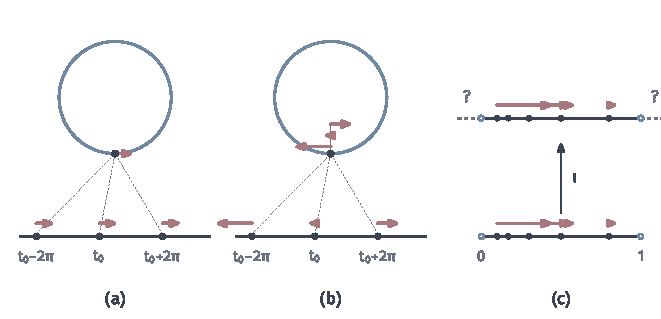
\includegraphics[width=112mm]{figures/04-spaces-measures-and-geometry/04-manifolds/matplotlib/mmaps-field-conflict/figure.pdf}
  \caption{逐点推送向量场。(a)$\frac{\mathrm d}{\mathrm dt}$在$E$的三个原像$t_0,t_0\pm2\pi$（$t_0=-\pi/2$）处推送结果一致。(b)$t\frac{\mathrm d}{\mathrm dt}$的三个推送结果不同；它们本来都在$E(t_0)$处，为看清而沿法向错开。箭头长度与$t$成正比。(c)包含映射$\iota$与场$\frac1t\frac{\mathrm d}{\mathrm dt}$：区间外没有原像（虚线），靠近$0$时箭头无限变长。}
  \label{fig:mmaps-field-conflict}
\end{BookInlineFigure}

\paragraph{$F$相关的向量场}
既然一般得不到目标上的向量场，就把问题反过来问：给定两侧的向量场，它们和$F$是否协调？这个提法不要求$F$单射或满射。

\begin{definition}[$F$相关]
\label{def:mmaps-f-related}
设$F:M\to N$光滑，$X\in\mathfrak X(M)$，$Y\in\mathfrak X(N)$。若对每个$p\in M$都有
\begin{equation}
\mathrm dF_p(X_p)=Y_{F(p)},
\label{eq:mmaps-f-related}
\end{equation}
则称$X$与$Y$是\term{$F$相关}（$F$-related）的。
\end{definition}

上面的例子中，$\frac{\mathrm d}{\mathrm dt}$与$\partial_\theta$是$E$相关的，而$t\frac{\mathrm d}{\mathrm dt}$不与$S^1$上任何向量场$E$相关。多个原像并不妨碍$F$相关，只要它们给出同一个值。

投影上有一个不平凡的例子。设$X$是球面的旋转场，在北极图中分量为$(-u_2,u_1)$；$Y$是平面上的旋转场，分量为$(-y_2,y_1)$。验证$p$和$q$两个原像，$p$处$\bm u=(0,3)$，$q$处$\bm u=(0,\tfrac13)$，分别代入
\[
\begin{aligned}
\operatorname{diag}(0.2,-0.16)\,(-3,\ 0)^\top&=(-0.6,\ 0)^\top,\\
\operatorname{diag}(1.8,1.44)\,(-\tfrac13,\ 0)^\top&=(-0.6,\ 0)^\top .
\end{aligned}
\]
两个结果相同，都等于$Y$在$(0,0.6)$处的值$(-0.6,0)$。这不是巧合：先转再投影等于先投影再转，$\pi$把球面上绕竖直轴的旋转变成平面上的旋转。

$F$相关还可以用向量场对函数的作用来刻画。这个刻画不涉及坐标，并且只用到向量场的代数作用，后面处理Lie括号时很方便。

\begin{lemma}[$F$相关的函数刻画]
\label{lem:mmaps-f-related-functions}
$X$与$Y$是$F$相关的，当且仅当对$N$的每个开子集$W$和每个$g\in C^\infty(W)$，在$F^{-1}(W)$上都有
\begin{equation}
X(g\circ F)=(Yg)\circ F .
\label{eq:mmaps-f-related-functions}
\end{equation}
\end{lemma}

\begin{proof}
在$p\in F^{-1}(W)$处，由链式法则\eqref{eq:mmaps-chain-rule}，
\[
X_p(g\circ F)=\mathrm d(g\circ F)_p(X_p)=\mathrm dg_{F(p)}\bigl(\mathrm dF_p(X_p)\bigr).
\]
而右端的$(Yg)(F(p))=\mathrm dg_{F(p)}(Y_{F(p)})$。若$X,Y$是$F$相关的，两者相等。

反过来，设两式对所有$g$相等。取$g$为$F(p)$附近图中的坐标函数$y_k$，$\mathrm dy_k$读出的是第$k$个分量，所以$\mathrm dF_p(X_p)$与$Y_{F(p)}$的第$k$个分量相等。对所有$k$成立，二者相等。
\end{proof}

用投影检验这个等式。取$g(\bm y)=y_2$，平面旋转场作用于它，$Yg=y_1$，于是右端的$(Yg)\circ\pi$是球面上的函数$y_1$。左端$g\circ\pi$是球面上的函数$y_2$，球面旋转场的速度是$(-y_2,y_1,0)$，所以$X(y_2)=y_1$，两端相等。

\begin{theorem}[$F$相关与Lie括号相容]
\label{thm:mmaps-f-related-bracket}
若$X_1$与$Y_1$、$X_2$与$Y_2$分别是$F$相关的，则$[X_1,X_2]$与$[Y_1,Y_2]$也是$F$相关的。
\end{theorem}

\begin{proof}
任取开集$W\subseteq N$与$g\in C^\infty(W)$。由引理~\ref{lem:mmaps-f-related-functions}，
\[
X_2(g\circ F)=(Y_2g)\circ F .
\]
两边再作用$X_1$，并对函数$Y_2g$用同一个引理，得到
\[
X_1X_2(g\circ F)=X_1\bigl((Y_2g)\circ F\bigr)=(Y_1Y_2g)\circ F .
\]
交换下标，得到另一个次序的等式，两式相减，
\[
[X_1,X_2](g\circ F)=([Y_1,Y_2]g)\circ F .
\]
再用一次引理的充分性，定理得证。
\end{proof}

用一个能手算的例子看定理在说什么。令$F:\mathbb R^2\to\mathbb R^2$，$F(x,y)=(x,\ y+x^2)$，目标的坐标记为$(a,b)$，Jacobian矩阵为
\[
\bm J_F=\begin{bmatrix}1&0\\2x&1\end{bmatrix}.
\]
取$X_1=\partial_x$，$X_2=x\,\partial_y$。逐列推送，再用$a=x$改写，得到与它们$F$相关的场：
\[
Y_1=\partial_a+2a\,\partial_b,\qquad Y_2=a\,\partial_b .
\]

分别计算两侧的括号。左侧只有$X_2$的系数依赖$x$，所以$[X_1,X_2]=\partial_y$，它的推送由$\bm J_F$的第二列给出，是$(0,1)^\top$，即$\partial_b$。右侧$Y_1$作用于$Y_2$的系数$a$得$1$，而$Y_2$作用于$Y_1$的系数$2a$得$0$，所以$[Y_1,Y_2]=\partial_b$，与推送结果相同。

\paragraph{双向光滑的双射}
若$F$是双射，每点恰有一个原像，上面的冲突和缺失都不会出现。若逆映射也光滑，推送所得的场还是光滑的。这类映射在第~\ref{chap:manifold-relations}章称为微分同胚，这里先说明它对向量场的作用。

\begin{theorem}[向量场的推送]
\label{thm:mmaps-pushforward-field}
设$F:M\to N$是光滑双射，且逆映射$F^{-1}$也光滑。对$X\in\mathfrak X(M)$，令
\begin{equation}
(F_*X)_q=\mathrm dF_{F^{-1}(q)}\bigl(X_{F^{-1}(q)}\bigr),\qquad q\in N .
\label{eq:mmaps-pushforward-field}
\end{equation}
则$F_*X$是$N$上的光滑向量场，并且是唯一与$X$为$F$相关的向量场。
\end{theorem}

\begin{proof}
$F$是双射，每个$q$有唯一原像，所以$F_*X$是良定义的向量场，并且按构造与$X$为$F$相关。任何与$X$为$F$相关的$Y$在$q=F(p)$处都必须等于$\mathrm dF_p(X_p)$，唯一性随之成立。

光滑性在坐标中检查。记$\hat X$为$X$的分量，在$q$附近的一对图中，$F_*X$的分量是
\[
\bm y\mapsto\bm J_{\hat F}\bigl(\widehat{F^{-1}}(\bm y)\bigr)\,\hat X\bigl(\widehat{F^{-1}}(\bm y)\bigr).
\]
$\widehat{F^{-1}}$光滑，$\bm J_{\hat F}$的元素与$\hat X$光滑，它们的复合与乘积仍光滑。
\end{proof}

逆映射光滑这个条件不能省。$F(x)=x^3$是$\mathbb R$到自身的光滑双射，它的逆映射$x^{1/3}$在原点不可微。推送$\frac{\mathrm d}{\mathrm dx}$，每点$x$处得到$3x^2\frac{\mathrm d}{\mathrm dy}$，用$x=y^{1/3}$写成目标坐标，
\[
(F_*X)_y=3y^{2/3}\,\frac{\mathrm d}{\mathrm dy}.
\]
分量$3y^{2/3}$在原点连续但有尖点，所以结果不光滑，见图~\ref{fig:mmaps-cube-field}。

\begin{BookInlineFigure}
  \centering
  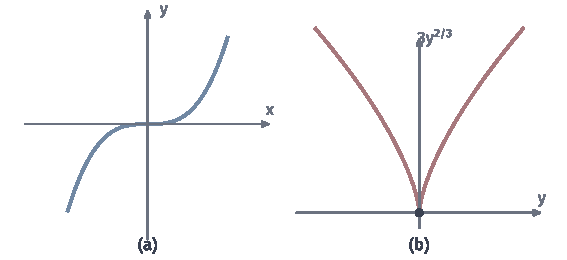
\includegraphics[width=96mm]{figures/04-spaces-measures-and-geometry/04-manifolds/matplotlib/mmaps-cube-field/figure.pdf}
  \caption{逆映射不光滑时的推送。(a)$F(x)=x^3$是光滑双射，在原点斜率为零。(b)$\frac{\mathrm d}{\mathrm dx}$的推送分量$3y^{2/3}$在$y=0$处出现尖点。}
  \label{fig:mmaps-cube-field}
\end{BookInlineFigure}

旋转$R_\theta$满足定理的条件，逆映射是$R_{-\theta}$。限制在$S^2\setminus\{N\}$上，北极图中$(R_\theta)_*X$的分量由式~\eqref{eq:mmaps-pushforward-field}给出：
\[
\bm u'\mapsto\bm R(\theta)\,\hat X\bigl(\bm R(-\theta)\bm u'\bigr).
\]

先取球面的旋转场，$\hat X(\bm u)=\bm R(\tfrac\pi2)\bm u$。平面旋转彼此可交换，三个旋转矩阵的转角相加，于是
\[
\bm R(\theta)\bm R(\tfrac\pi2)\bm R(-\theta)\bm u'=\bm R(\tfrac\pi2)\bm u'.
\]
旋转场被推送为自身：绕竖直轴转动，不改变绕竖直轴转动的速度场。

再取常分量场$\partial_{u_1}$，$\hat X=\bm e_1$。代入后结果不依赖$\bm u'$，
\[
\bm R(\theta)\bm e_1=(\cos\theta,\ \sin\theta)^\top ,
\]
也就是
\[
(R_\theta)_*\partial_{u_1}=\cos\theta\,\partial_{u_1}+\sin\theta\,\partial_{u_2}.
\]
整片箭头跟着转了$\theta$，见图~\ref{fig:mmaps-rotation-field-push}。

\begin{BookInlineFigure}
  \centering
  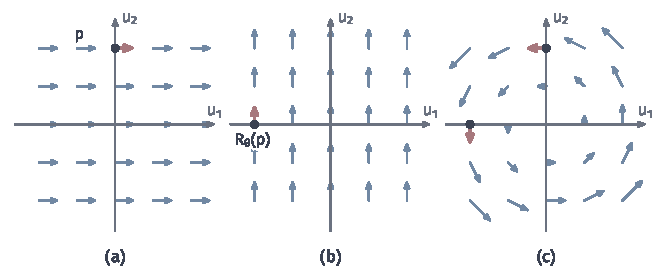
\includegraphics[width=112mm]{figures/04-spaces-measures-and-geometry/04-manifolds/matplotlib/mmaps-rotation-field-push/figure.pdf}
  \caption{旋转$R_\theta$（$\theta=\pi/2$）在北极图中推送向量场。(a)常分量场$\partial_{u_1}$（蓝），红箭头是$p$处的值。(b)推送结果$\partial_{u_2}$，$p$处的红箭头被送到$R_\theta(p)$处。(c)旋转场$(-u_2,u_1)$，推送后不变，红箭头是$p$与$R_\theta(p)$处的值，箭头长度按$0.28$缩放。}
  \label{fig:mmaps-rotation-field-push}
\end{BookInlineFigure}

\section{协向量的拉回}
\label{sec:mmaps-pullback}

切向量随映射向前推，从$p$处送到$F(p)$处。余切向量是对切向量的读数，它的换算方向恰好相反：如果已经知道怎样在$F(p)$处读数，就可以先把$p$处的切向量推过去，再在那里读数，这样得到的是$p$处的一个读数。本节把这个想法写成定义，并说明方向相反带来的好处。

\paragraph{逐点的拉回}
设$F:M\to N$光滑，$p\in M$，$\omega\in T^*_{F(p)}N$。对$\bm v\in T_pM$，$\mathrm dF_p(\bm v)$属于$T_{F(p)}N$，可以被$\omega$读取。

\begin{definition}[余切向量的拉回]
\label{def:mmaps-covector-pullback}
$\mathrm dF_p$的对偶映射
\[
(\mathrm dF_p)^*:T^*_{F(p)}N\to T^*_pM,\qquad
\bigl((\mathrm dF_p)^*\omega\bigr)(\bm v)=\omega\bigl(\mathrm dF_p(\bm v)\bigr)
\]
称为$F$在$p$处的余切映射，$(\mathrm dF_p)^*\omega$称为$\omega$的\term{拉回}（pullback）。
\end{definition}

右端对$\bm v$线性，所以$(\mathrm dF_p)^*\omega$确实是$p$处的余切向量；它对$\omega$也线性。在坐标中，设$\omega=\sum_kb_k\,\mathrm dy_k|_{F(p)}$，$\bm J=\bm J_{\hat F}(\varphi(p))$。把$(\mathrm dF_p)^*\omega$作用在$\partial_j|_p$上，由式\eqref{eq:mmaps-differential-basis}得到它的第$j$个系数$\sum_kb_k\,\partial\hat F_k/\partial x_j$。写成列向量，
\begin{equation}
\bm a=\bm J^\top\bm b .
\label{eq:mmaps-pullback-coordinates}
\end{equation}
切向量的分量用$\bm J$从$M$推到$N$，余切向量的系数用$\bm J^\top$从$N$拉回$M$，两个方向相反。

\paragraph{协向量场的拉回总有定义}
对$N$上的协向量场$\omega$，在每个$p\in M$处拉回$F(p)$处的值，得到$M$上的协向量场
\[
(F^*\omega)_p=(\mathrm dF_p)^*\bigl(\omega_{F(p)}\bigr),\qquad p\in M .
\]
这里每个$p$只需要一个值$\omega_{F(p)}$，它总是存在且唯一。所以向量场推送时遇到的两类困难都不出现：多个原像只是各自拉回同一个值，没有原像的点在$M$中根本不出现。在坐标中，$F^*\omega$的系数是$\bm J_{\hat F}(\bm x)^\top\hat{\bm b}(\hat F(\bm x))$，由光滑函数复合、相乘得到，所以$\omega$光滑时$F^*\omega$也光滑。拉回对任何光滑映射都适用，不需要$F$可逆。

\paragraph{运算规则}
拉回与函数、复合和微分的关系可以归结为三条规则。

\begin{theorem}[拉回的运算规则]
\label{thm:mmaps-pullback-rules}
设$F:M\to N$与$G:N\to P$光滑，$\omega$是$N$上的光滑协向量场，$g,f\in C^\infty(N)$。则
\begin{enumerate}
\item $F^*(g\,\omega)=(g\circ F)\,F^*\omega$；
\item $(G\circ F)^*=F^*\circ G^*$；
\item $F^*(\mathrm df)=\mathrm d(f\circ F)$。
\end{enumerate}
\end{theorem}

\begin{proof}
第一条：在$p$处，$g\,\omega$的值是$g(F(p))\,\omega_{F(p)}$，对偶映射线性，系数$g(F(p))$直接提出。第二条：由链式法则，$\mathrm d(G\circ F)_p=\mathrm dG_{F(p)}\circ\mathrm dF_p$；对偶映射交换复合次序，$(\mathrm d(G\circ F)_p)^*=(\mathrm dF_p)^*\circ(\mathrm dG_{F(p)})^*$。第三条：对$\bm v\in T_pM$，
\[
\bigl(F^*\mathrm df\bigr)_p(\bm v)=\mathrm df_{F(p)}\bigl(\mathrm dF_p(\bm v)\bigr)=\mathrm d(f\circ F)_p(\bm v),
\]
最后一步是链式法则应用于$f\circ F$。
\end{proof}

第三条说明“先微分再拉回”与“先复合再微分”给出同一个结果。复合次序在第二条中反过来：先作用$F$再作用$G$的映射，拉回时先用$G^*$再用$F^*$。这与切向量的推送$\mathrm d(G\circ F)=\mathrm dG\circ\mathrm dF$方向相反，是对偶映射的一般性质。

\paragraph{例子：圆周上的角度读数}
圆周上的两张角度图相差常数平移，所以$\mathrm d\theta_1$与$\mathrm d\theta_2$在重叠处相等，拼成整个圆周上的光滑协向量场，记为$\mathrm d\theta$。注意它不是某个全局光滑函数的微分，因为圆周上没有处处光滑的全局角度函数，记号只表示它在每张图中都是坐标函数的微分。

用$E(t)=(\cos t,\sin t)$拉回：$E$在角度图中的坐标表示是$t\mapsto t+c$，导数为$1$，由式\eqref{eq:mmaps-pullback-coordinates}，$E^*(\mathrm d\theta)=\mathrm dt$。这里$E$不是单射，每个圆周上的点有无穷多个原像，拉回照样良定义。这一计算也证实了上一段的断言：若$\mathrm d\theta=\mathrm df$对某个$f\in C^\infty(S^1)$成立，则由第三条规则$\mathrm d(f\circ E)=E^*\mathrm d\theta=\mathrm dt$，于是$f(E(t))=t+c$；但$f\circ E$以$2\pi$为周期，矛盾。与上一节对比，$\mathbb R$上的向量场$t\frac{\mathrm d}{\mathrm dt}$无法推送到圆周，而圆周上的协向量场总能拉回$\mathbb R$。

\paragraph{例子：旋转下的高度读数}
由运算规则的第三条，$R_\theta^*(\mathrm dh)=\mathrm d(h\circ R_\theta)=\mathrm dh$，因为旋转不改变高度。这与上一节在$p=(0,\tfrac35,\tfrac45)$处的矩阵计算是同一件事：那里用行向量左乘$\bm R(\theta)$，正是式\eqref{eq:mmaps-pullback-coordinates}的转置形式。用拉回的语言，计算不需要逐点核对，直接由函数的不变性得出。

\paragraph{向更一般对象的推广}
本节只拉回了余切向量，即对单个切向量的线性读数。同样的思路可以用于同时读取多个切向量的多重线性读数，例如面积元和体积元，其中最重要的是交替的情形，即微分形式。它们的拉回、外微分及与积分的关系，在第~\ref{chap:manifold-calculus}章定义交替形式之后建立；黎曼度量作为对两个切向量的对称读数，其拉回在第~\ref{chap:riemannian-geometry}章用于定义等距映射。

\section{本章小结}
\label{sec:mmaps-summary}

本章开头问：给定流形之间的映射，它怎样对应点，又怎样改变点处的方向和读数？对点而言，光滑映射由两侧坐标图中的坐标表示判断，换用相容的图不改变结论。同一个坐标公式可能描述两件事：同一点在两张图中的记录之间的换算，或者把点实际送到另一个点；前者是恒等映射的坐标表示，后者才移动了点。曲线和实值函数都是光滑映射的特例。

对方向而言，映射的微分$\mathrm dF_p:T_pM\to T_{F(p)}N$把经过$p$的曲线速度推送为经过$F(p)$的曲线速度，在坐标基下的矩阵是坐标表示的Jacobian矩阵；边界点处用光滑延拓的Jacobian矩阵，结果与延拓无关。链式法则$\mathrm d(G\circ F)_p=\mathrm dG_{F(p)}\circ\mathrm dF_p$成立，秩不依赖图，实值函数的微分与第~\ref{chap:manifold-basics}章的余切向量$\mathrm df_p$一致。

对整个向量场逐点推送时，不同原像可能给出同一点处相互冲突的向量，像以外的点没有值，所以一般映射不能把向量场推送成目标上的向量场。能做的是判断两侧的场是否$F$相关，它等价于$X(g\circ F)=(Yg)\circ F$，并与Lie括号相容。若映射是光滑双射且逆映射光滑，推送得到唯一的光滑向量场；逆映射不光滑时，例如$x\mapsto x^3$，推送结果可能不光滑。

对读数而言，余切向量沿相反方向拉回：$(\mathrm dF_p)^*\omega=\omega\circ\mathrm dF_p$，坐标中由Jacobian矩阵的转置给出。协向量场的拉回对任何光滑映射都有定义，因为每个原像点只需要一个目标值；它满足$(G\circ F)^*=F^*\circ G^*$与$F^*(\mathrm df)=\mathrm d(f\circ F)$。推送与拉回的方向不同、作用对象不同，所需的条件也不同。

这些都是映射的局部操作。微分可逆、单射或满射分别说明映射在一点附近保留或覆盖了多少方向，但不能单独决定两个流形整体上是否等价，或一个流形的像能否成为子流形。第~\ref{chap:manifold-relations}章在本章的微分与秩的基础上，加入可逆性与拓扑条件来回答这些问题。


\chapter{流形之间的关系}
\label{chap:manifold-relations}

球面与椭球面看起来不同，一个圆，一个扁；可是把椭球面沿三个坐标轴分别缩放，就能毫无撕裂、毫无折叠地变成球面，反过来也一样。另一方面，圆周放在平面里是一条光滑的闭曲线，而一条在原点自交的“8”字形曲线，虽然也是由光滑参数化画出来的，却在交叉点处不像一段曲线。前一个例子问的是两个流形是否“本质上相同”，后一个问的是一个对象能否作为另一个流形中的光滑子流形。

上一章已经能计算映射的微分和秩。本章用这些工具研究流形之间的两种关系。第~\ref{sec:mrel-diffeomorphisms}节用微分同胚表达两个流形具有相同的光滑结构，并说明微分可逆只给出局部的可逆性。第~\ref{sec:mrel-local-structure}节考察映射在一点附近的结构：微分处处单射的浸入保留方向，处处满射的淹没覆盖方向；在秩保持不变的邻域中，常秩定理把映射化为最简单的坐标形式。

局部结构还不足以描述包含关系，“8”字形曲线就是局部处处保留方向、整体却不像子空间的例子。第~\ref{sec:mrel-embedded-submanifolds}节因此在浸入之上加入到像的同胚条件，得到嵌入，再用一部分坐标取零的局部模型刻画嵌入子流形，最后说明约束方程的微分满秩时，水平集自动成为这样的子流形；球面和正交矩阵组成的集合都由此得到。

本章只讨论无边界流形。带边界时，反函数定理在边界点处需要另外的处理，相应结论另核条件，只在必要处说明。微分同胚保持光滑结构，但不保持长度：区间$(0,1)$与整条实轴微分同胚，长度却一个有限、一个无限。比较长度和距离的等距关系，要在第~\ref{chap:riemannian-geometry}章引入黎曼度量之后讨论。

\section{微分同胚}
\label{sec:mrel-diffeomorphisms}

两个流形什么时候应当看作“同一个”光滑流形？集合论只问元素能否一一对应，拓扑只问邻近关系能否一一对应，而光滑流形还带有光滑结构，即哪些函数光滑、哪些曲线有速度。要说两个流形在光滑意义下相同，就要求有一个对应把这些信息双向保留下来。

\paragraph{定义}
保留光滑结构，意味着对应本身光滑，并且反过来的对应也光滑。

\begin{definition}[微分同胚]
\label{def:mrel-diffeomorphism}
设$M,N$是光滑流形。若$F:M\to N$是光滑双射，且逆映射$F^{-1}:N\to M$也光滑，则称$F$为\term{微分同胚}（diffeomorphism）。存在微分同胚时，称$M$与$N$微分同胚。
\end{definition}

微分同胚$F$把$N$上的光滑函数$g$对应到$M$上的光滑函数$g\circ F$，反过来$f\mapsto f\circ F^{-1}$，两种对应互逆。所以在两个流形上能谈论的“光滑对象”完全相同，只是名字换了。第~\ref{chap:manifold-maps}章又说明，光滑双射且逆光滑的映射把向量场一一推送为光滑向量场，所以微分同胚也保留了向量场。

\paragraph{三种对应的比较}
集合双射、同胚与微分同胚依次保留越来越多的信息，可以用例子看清每一层多出了什么。

只是集合双射，几乎什么都不保留。$\mathbb R$与$\mathbb R^2$的元素可以一一对应，但这样的双射不可能是同胚，因为维数是拓扑不变量；这一维数不变性需要较深的拓扑工具，这里不给出证明。同胚保留连通性、紧性这类拓扑性质，但不保留光滑性。$F(x)=x^3$是$\mathbb R$到自身的同胚，也是光滑双射，但逆映射$x^{1/3}$在原点不可微，所以$F$不是微分同胚。在$F$下，光滑函数$g(y)=y$对应到$g\circ F^{-1}$即$x^{1/3}$，不再光滑。

微分同胚是比较两个光滑结构的正确工具，而不是比较两个图册的写法。第~\ref{chap:manifold-basics}章指出，$\mathbb R$上的图$\chi(x)=x^3$与恒等图不光滑相容，记带$\chi$所决定结构的实轴为$\mathbb R_\chi$。恒等映射$\mathbb R\to\mathbb R_\chi$是同胚，但不是微分同胚。可是$G(x)=x^{1/3}$是从标准$\mathbb R$到$\mathbb R_\chi$的微分同胚：坐标表示是$\chi\circ G(x)=x$，逆映射的坐标表示是$G^{-1}\circ\chi^{-1}(z)=(z^{1/3})^3=z$，都光滑。所以这两个光滑结构不同，得到的光滑流形却微分同胚。

\paragraph{微分同胚的微分可逆}
微分同胚在每点的微分都是线性同构，这是链式法则的直接推论，也说明微分同胚的流形维数相同。

\begin{theorem}[微分同胚的微分]
\label{thm:mrel-diffeo-differential}
若$F:M\to N$是微分同胚，则对每个$p\in M$，$\mathrm dF_p:T_pM\to T_{F(p)}N$是线性同构，其逆为$\mathrm d(F^{-1})_{F(p)}$。特别地，$\dim M=\dim N$。
\end{theorem}

\begin{proof}
对$F^{-1}\circ F=\mathrm{id}_M$与$F\circ F^{-1}=\mathrm{id}_N$分别用链式法则，得$\mathrm d(F^{-1})_{F(p)}\circ\mathrm dF_p=\mathrm{id}_{T_pM}$与$\mathrm dF_p\circ\mathrm d(F^{-1})_{F(p)}=\mathrm{id}_{T_{F(p)}N}$。两个有限维空间之间存在互逆的线性映射，维数相同。
\end{proof}

\paragraph{反函数定理}
反过来，若只知道$\mathrm dF_p$可逆，能推出什么？在欧氏空间中，局部反函数定理说：Jacobian矩阵在一点可逆的连续可微映射，在该点附近有连续可微的逆。这一定理及隐函数定理可参考\BookChapterRef{chap:implicit-inverse-functions}{卷二第19章“隐函数与反函数”}；光滑映射的逆映射也光滑，因为逆映射的Jacobian矩阵$[\bm J_G]^{-1}$是光滑函数的复合，逐阶求导即可。借助坐标图，这一结论搬到流形上。

\begin{theorem}[流形上的反函数定理]
\label{thm:mrel-inverse-function}
设$M,N$是无边界光滑流形，$F:M\to N$光滑，$p\in M$，且$\mathrm dF_p$可逆。则存在$p$的开邻域$U$与$F(p)$的开邻域$V$，使$F|_U:U\to V$是微分同胚。
\end{theorem}

\begin{proof}
取包含$p$与$F(p)$的图，使$F(U_1)\subseteq V_1$。坐标表示$\hat F$在$\varphi(p)$处的Jacobian矩阵就是$\mathrm dF_p$的矩阵，可逆，于是两侧维数相同。由欧氏反函数定理，存在$\varphi(p)$的开邻域$\widehat U$与$\hat F(\varphi(p))$的开邻域$\widehat V$，使$\hat F:\widehat U\to\widehat V$是光滑双射且逆光滑。令$U=\varphi^{-1}(\widehat U)$，$V=\psi^{-1}(\widehat V)$，则$F|_U=\psi^{-1}\circ\hat F\circ\varphi$是三个微分同胚的复合。
\end{proof}

$\varphi(p)$在$\varphi(U_1)$的内部是这里不可缺少的。在半空间的边界点处，坐标表示的值域可能被迫落在半空间中，欧氏反函数定理给出的开邻域不再适用，所以本章把讨论限制在无边界情形。

\paragraph{局部可逆与整体双射}
若$F$在每点都满足定理~\ref{thm:mrel-inverse-function}的条件，就称它为\term{局部微分同胚}（local diffeomorphism）。局部微分同胚未必是微分同胚，因为反函数定理只给出局部的逆，不涉及整体是否一一对应。

映射$E:\mathbb R\to S^1$，$E(t)=(\cos t,\sin t)$，在角度图中坐标表示的导数为$1$，所以是局部微分同胚；但$E(t)=E(t+2\pi)$，它不是单射。圆周上的倍角映射$(\cos\theta,\sin\theta)\mapsto(\cos2\theta,\sin2\theta)$在角度坐标中是$\theta\mapsto2\theta$（相差$2\pi$的整数倍），导数为$2$，也是局部微分同胚，并且是满射，可每点恰有两个原像。这两个例子说明，导数处处可逆既不推出单射，也与满射无关。

缺的正是整体的一一对应。若局部微分同胚$F$还是双射，它就是微分同胚：逆映射$F^{-1}$在每点$q$附近与反函数定理给出的局部逆一致，局部逆光滑，所以$F^{-1}$光滑。类似地，单射的局部微分同胚是到其像的微分同胚，并且像是开集，因为每点的像都含有一个开邻域。

\paragraph{光滑结构相同不等于几何相同}
微分同胚只关心光滑结构，不关心长度与距离。映射$x\mapsto\tan(\pi(x-\tfrac12))$是$(0,1)$到$\mathbb R$的微分同胚，导数$\pi/\cos^2(\pi(x-\tfrac12))$处处为正，逆映射$y\mapsto\tfrac12+\tfrac1\pi\arctan y$也光滑。前者长度为$1$，后者无界。再如$x\mapsto2x$是$\mathbb R$到自身的微分同胚，把所有距离加倍。所以微分同胚的两个流形可以有完全不同的度量性质。保持长度的映射需要在切空间上先有内积，这样的等距映射在第~\ref{chap:riemannian-geometry}章讨论。

\section{映射的局部结构}
\label{sec:mrel-local-structure}

要判断一个映射的像或原像能否成为光滑子流形，先要看映射在一点附近怎样作用于方向。微分可能把非零的切向量送到零，丢失方向；可能达不到目标的全部方向；还可能在附近各点的秩不同。本节的$M,N$都是无边界光滑流形，维数分别为$m,n$，整体的拓扑条件留到下一节。

\subsection{浸入与淹没}
\label{sec:mrel-immersion-submersion}

\paragraph{定义}
线性代数里，矩阵的列线性无关时对应的映射是单射，行线性无关时是满射。下面两个矩阵分别属于这两类：
\[
\begin{bmatrix}1&0\\0&1\\1&1\end{bmatrix},\qquad
\begin{bmatrix}1&0&1\\0&1&1\end{bmatrix}.
\]
第一个是$3\times2$矩阵，秩为$2$，把$\mathbb R^2$单射地送进$\mathbb R^3$；第二个是$2\times3$矩阵，秩为$2$，把$\mathbb R^3$满射地压到$\mathbb R^2$上。对映射在每一点的微分提出这两种要求，就得到两类映射。

\begin{definition}[浸入与淹没]
\label{def:mrel-immersion-submersion}
设$F:M\to N$光滑。若对每个$p\in M$，$\mathrm dF_p$都是单射，则称$F$为\term{浸入}（immersion）；若对每个$p\in M$，$\mathrm dF_p$都是满射，则称$F$为\term{淹没}（submersion）。
\end{definition}

浸入不丢失方向：经过$p$的两个不同速度被送到$F(p)$处的两个不同速度。淹没覆盖方向：$F(p)$处的任何速度都是某个$p$处速度的像。用秩表达，浸入在每点秩为$m$，淹没在每点秩为$n$。

单射要求$m\leq n$，满射要求$m\geq n$，所以浸入只能从低维到高维或同维，淹没只能从高维到低维或同维。同维时两者一致，由反函数定理都等价于局部微分同胚。

\paragraph{例子}
曲线$\gamma:I\to M$是浸入，当且仅当速度处处非零。图~\ref{fig:mrel-cusp-velocity}比较了两条平面曲线。$E(t)=(\cos t,\sin t)$作为$\mathbb R\to\mathbb R^2$的映射，速度$(-\sin t,\cos t)$的长度恒为$1$，处处非零，是浸入。

$\beta(t)=(t^2,t^3)$的速度是$(2t,3t^2)$，在$t=0$处为零，不是浸入。它的像是曲线$y_2^2=y_1^3$，在原点有一个尖点。接近原点时速度越来越小，曲线的方向在原点处从一支突然转到另一支，这正是速度为零允许发生的事。

\begin{BookInlineFigure}
  \centering
  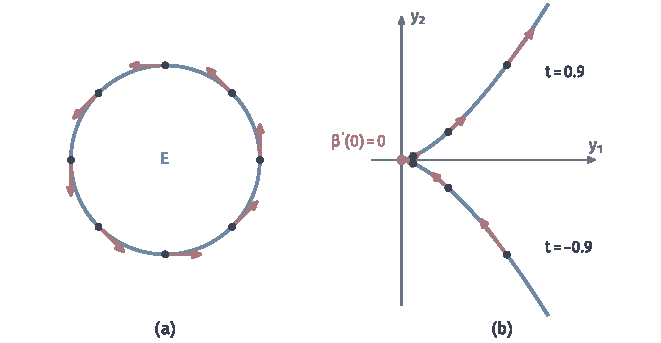
\includegraphics[width=112mm]{figures/04-spaces-measures-and-geometry/04-manifolds/matplotlib/mrel-cusp-velocity/figure.pdf}
  \caption{速度是否为零。(a)$E(t)=(\cos t,\sin t)$的速度（红箭头）长度恒为$1$，$E$是浸入。(b)$\beta(t)=(t^2,t^3)$在$t=\pm0.3,\pm0.6,\pm0.9$处的速度按真实长度的$0.12$倍画出，越接近原点越短；原点处速度为零，曲线出现尖点。}
  \label{fig:mrel-cusp-velocity}
\end{BookInlineFigure}

高维的浸入也可以手算。北极球极投影的逆把坐标$\bm u=(u_1,u_2)$送到$\mathbb R^3$，记$\rho=u_1^2+u_2^2$，
\[
\sigma_N^{-1}(\bm u)=\frac{(2u_1,\ 2u_2,\ \rho-1)}{\rho+1}.
\]
在$\bm u=(0,3)$处，第一列已在第~\ref{chap:manifold-basics}章算出是$(\tfrac15,0,0)$。第二列对$u_2$求导，三个分量分别是
\[
\frac{-4u_1u_2}{(\rho+1)^2}=0,\qquad
\frac{2(\rho+1)-4u_2^2}{(\rho+1)^2}=-\frac4{25},\qquad
\frac{4u_2}{(\rho+1)^2}=\frac3{25}.
\]

于是在这一点的Jacobian矩阵及其秩是
\[
\bm J=\begin{bmatrix}1/5&0\\0&-4/25\\0&3/25\end{bmatrix},\qquad \operatorname{rank}\bm J=2.
\]
两列正是切向量$\bm v$与$\bm w$，这个$3\times2$矩阵列满秩，所以$\sigma_N^{-1}$在这一点是单射的微分。

淹没的例子是投影。取前$n$个坐标的映射$\pi:\mathbb R^m\to\mathbb R^n$，$m\geq n$，Jacobian矩阵是$[\bm I_n\ \bm 0]$，行满秩。球面上的高度函数$h$是更有几何意味的例子，它在北极图中的表示和微分系数是
\[
h\circ\sigma_N^{-1}(\bm u)=\frac{\rho-1}{\rho+1},\qquad
\mathrm dh=\frac{4u_1\,\mathrm du_1+4u_2\,\mathrm du_2}{(\rho+1)^2}.
\]

在$\bm u=(0,3)$处系数是$(0,0.12)$，非零，秩为$1$。在$\bm u=\bm 0$（南极）处系数全为零，秩为$0$；北极由南极图同样算出秩为$0$。所以$h:S^2\to\mathbb R$不是淹没，但限制到$S^2\setminus\{N,S\}$上就是淹没。

图~\ref{fig:mrel-height-rank}读出同一件事的几何含义。在$p$处，沿纬线的方向$\bm e_1=(1,0,0)$不改变高度，构成微分的核；沿经线向下的单位方向$\bm e_2=(0,0.8,-0.6)$让高度以$-0.6$的速率变化，覆盖了$\mathbb R$的全部方向。淹没的等值集正是纬线这样的一维曲线，维数$2-1=1$。

\begin{BookInlineFigure}
  \centering
  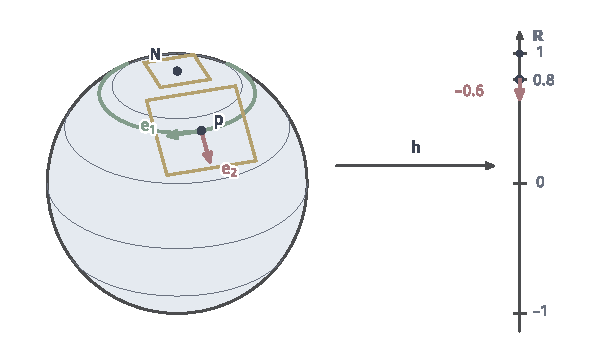
\includegraphics[width=104mm]{figures/04-spaces-measures-and-geometry/04-manifolds/matplotlib/mrel-height-rank/figure.pdf}
  \caption{高度函数$h(\bm y)=y_3$在$S^2$上的秩。在$p=(0,\tfrac35,\tfrac45)$处，绿色的纬线方向$\bm e_1$属于$\ker\mathrm dh_p$，红色的方向$\bm e_2$被送到$\mathbb R$上长度$0.6$的向量（两侧都按真实长度的$0.3$倍画出）。在北极$N$处切平面水平，$\mathrm dh_N=0$，所有方向都被送到零。}
  \label{fig:mrel-height-rank}
\end{BookInlineFigure}

\paragraph{微分的单射、满射与映射的单射、满射}
浸入与淹没都是逐点关于微分的条件，不涉及映射本身是否单射或满射。表~\ref{tab:mrel-injective-comparison}列出了四个例子，说明这两组概念互相独立，判断时要分清问的是方向还是点。

\begin{BookInlineTable}
  \centering
  \begin{tabular}{lll}
    \toprule
    映射 & 映射本身 & 微分\\
    \midrule
    $E:\mathbb R\to\mathbb R^2$ & 非单射（周期$2\pi$） & 处处单射\\
    $\beta(t)=(t^2,t^3)$ & 单射 & 在$t=0$处不单射\\
    $h:S^2\setminus\{N,S\}\to\mathbb R$ & 非满射（像为$(-1,1)$） & 处处满射\\
    $x\mapsto x^3$ & 满射 & 在原点不满射\\
    \bottomrule
  \end{tabular}
  \caption{映射的单射、满射与微分的单射、满射互相独立。}
  \label{tab:mrel-injective-comparison}
\end{BookInlineTable}

\subsection{常秩定理}
\label{sec:mrel-constant-rank}

\paragraph{一点的秩与邻域中的秩}
线性代数告诉我们，任何秩为$r$的矩阵$\bm A$，在定义域和值域各选一组合适的基之后，都成为最简单的形式：存在可逆矩阵$\bm P,\bm Q$，使
\[
\bm P\bm A\bm Q=\begin{bmatrix}\bm I_r&\bm 0\\\bm 0&\bm 0\end{bmatrix}.
\]
选基换成选坐标，我们希望非线性映射也能写成$(x_1,\ldots,x_r,0,\ldots,0)$这样的形式。

类比在这里遇到了线性代数没有的问题：Jacobian矩阵随点变化，矩阵的秩也可能随点变化。一点的秩控制附近秩的下限，却不控制上限。若$\mathrm dF_p$的秩为$r$，Jacobian矩阵有一个非零的$r$阶子式，子式是偏导数的多项式，连续，所以在$p$附近仍非零，附近各点的秩至少为$r$。

秩却可以在$p$附近变大。$f(x)=x^2$在$0$处秩为$0$，在其余点秩为$1$。若它在$0$附近有秩$1$的标准形式$x\mapsto x$，就应当局部单射；若有秩$0$的标准形式，就应当局部为常值。这两者都不成立，因为$f(1/k)=f(-1/k)$，而$f$又不是常值。可见只看一点的秩，得不到局部形式。

二维的例子也一样。令$F(x,y)=(x,xy)$，Jacobian矩阵和行列式分别是
\[
\bm J_F=\begin{bmatrix}1&0\\y&x\end{bmatrix},\qquad \det\bm J_F=x.
\]
在$x=0$处秩为$1$，在$x\neq0$处秩为$2$。球面的高度函数也是如此：在两极秩为$0$，在附近的点秩为$1$，所以两极附近不能用单一的标准形式描述。

有一个重要的例外是满秩。秩不能超过$\min(m,n)$，若$p$处的秩已经达到$\min(m,n)$，附近的秩既不小于它，也不能更大，只能保持不变。所以对浸入和淹没，一点满秩就推出邻域常秩，下面的定理对它们自动适用。

\paragraph{定理与证明}
常秩条件下，映射在适当的坐标中就是线性映射的标准形式。证明的想法是用反函数定理逐步“拉直”：先在源中换坐标，使映射的前$r$个分量变成坐标本身；再由秩的上限，说明其余分量只依赖前$r$个坐标；最后在目标中换坐标，把其余分量减掉。

\begin{theorem}[常秩定理]
\label{thm:mrel-constant-rank}
设$F:M\to N$光滑，$p\in M$，$F$在$p$的某个邻域中各点的秩都等于$r$。则存在以$p$为中心的图$(U,\varphi)$与以$F(p)$为中心的图$(V,\psi)$，$F(U)\subseteq V$，使
\begin{equation}
\psi\circ F\circ\varphi^{-1}(x_1,\ldots,x_r,x_{r+1},\ldots,x_m)=(x_1,\ldots,x_r,0,\ldots,0).
\label{eq:mrel-constant-rank-form}
\end{equation}
\end{theorem}

\begin{proof}
取两侧的图，可设$F$是欧氏开集$W\subseteq\mathbb R^m$到$\mathbb R^n$的光滑映射，$p=\bm 0$，$F(\bm 0)=\bm 0$，并且在$W$上秩恒为$r$。$\bm J_F(\bm 0)$有一个非零的$r$阶子式，重排两侧坐标的次序，可设它位于左上角。

把变量写成$\bm x=(\bm x',\bm x'')$，$\bm x'\in\mathbb R^r$，并把$F$写成$(Q,R)$，其中$Q$取值于$\mathbb R^r$。于是$\partial Q/\partial\bm x'(\bm 0)$可逆。

第一步，在源中换坐标。令$G(\bm x)=(Q(\bm x),\bm x'')$，它在$\bm 0$处的Jacobian矩阵是
\[
\bm J_G(\bm 0)=\begin{bmatrix}\partial Q/\partial\bm x'(\bm 0)&\partial Q/\partial\bm x''(\bm 0)\\\bm 0&\bm I_{m-r}\end{bmatrix},
\]
行列式等于$\det\partial Q/\partial\bm x'(\bm 0)\neq0$。由反函数定理，$G$把$\bm 0$的某个邻域微分同胚地映到$\bm 0$的一个邻域，缩小后可设后者是开方体$C$。

在$C$上有$G\circ G^{-1}=\mathrm{id}$，比较前$r$个分量得$Q(G^{-1}(\bm z))=\bm z'$，所以
\[
F\circ G^{-1}(\bm z)=\bigl(\bm z',\,\widetilde R(\bm z)\bigr),\qquad \widetilde R=R\circ G^{-1}.
\]

第二步，利用秩的上限。$F\circ G^{-1}$的Jacobian矩阵是
\[
\begin{bmatrix}\bm I_r&\bm 0\\\partial\widetilde R/\partial\bm z'&\partial\widetilde R/\partial\bm z''\end{bmatrix}.
\]
$G^{-1}$是微分同胚，所以这个矩阵的秩恒等于$r$。前$r$行已经贡献了秩$r$，若右下块有非零元素，秩就至少为$r+1$，于是
\[
\frac{\partial\widetilde R}{\partial\bm z''}\equiv\bm 0.
\]
$C$是方体，固定$\bm z'$时$\bm z''$在一个凸集中变化，所以$\widetilde R(\bm z)=S(\bm z')$只依赖$\bm z'$。

第三步，在目标中换坐标。令
\[
T(\bm y',\bm y'')=\bigl(\bm y',\ \bm y''-S(\bm y')\bigr),
\]
定义在$\bm y'$属于$C$在前$r$个坐标上的投影的开集上。它光滑，逆为$(\bm y',\bm y''+S(\bm y'))$，也光滑。代入后得到
\[
T\circ F\circ G^{-1}(\bm z)=\bigl(\bm z',\ S(\bm z')-S(\bm z')\bigr)=(\bm z',\bm 0).
\]
取源中的新坐标为$G$，目标中的新坐标为$T$，并缩小邻域使$F(U)\subseteq V$，即得所需形式。
\end{proof}

\paragraph{例子：一步步拉直}
证明中的三步可以在一个具体映射上完整走一遍。令$F:\mathbb R^2\to\mathbb R^2$，
\[
F(x_1,x_2)=(s,s^2),\qquad s=x_1+x_2.
\]
它的Jacobian矩阵第二行是第一行的$2s$倍：
\[
\bm J_F=\begin{bmatrix}1&1\\2s&2s\end{bmatrix},\qquad\operatorname{rank}\bm J_F=1.
\]
所以秩处处等于$1$，常秩定理适用，$r=1$。

这里$Q(x_1,x_2)=x_1+x_2$，$R(x_1,x_2)=(x_1+x_2)^2$，$\partial Q/\partial x_1=1\neq0$。第一步在源中换坐标，
\[
G(x_1,x_2)=(x_1+x_2,\ x_2),\qquad G^{-1}(z_1,z_2)=(z_1-z_2,\ z_2).
\]

把$G^{-1}$代入$F$，第一个分量变成坐标$z_1$，第二个分量自动只依赖$z_1$：
\[
F\circ G^{-1}(z_1,z_2)=(z_1,\ z_1^2).
\]
也就是说第二步中的$S(z_1)=z_1^2$，这里无需额外计算，因为$F$本来就沿直线$x_1+x_2=$常数取常值。第三步在目标中减去$S$，
\[
T(y_1,y_2)=(y_1,\ y_2-y_1^2),\qquad T\circ F\circ G^{-1}(z_1,z_2)=(z_1,0).
\]

图~\ref{fig:mrel-rank-steps}跟踪了点$(1,2)$：$F$把它送到$(3,9)$，$G$把它送到$(3,2)$，$T$把$(3,9)$送到$(3,0)$，而$(z_1,z_2)=(3,2)$在标准形式下正好变成$(3,0)$。图中可以看到映射的结构：源上的等值线是一族平行直线，目标上的像是一条抛物线，换坐标只是把直线摆正、把抛物线压平。

\begin{BookInlineFigure}
  \centering
  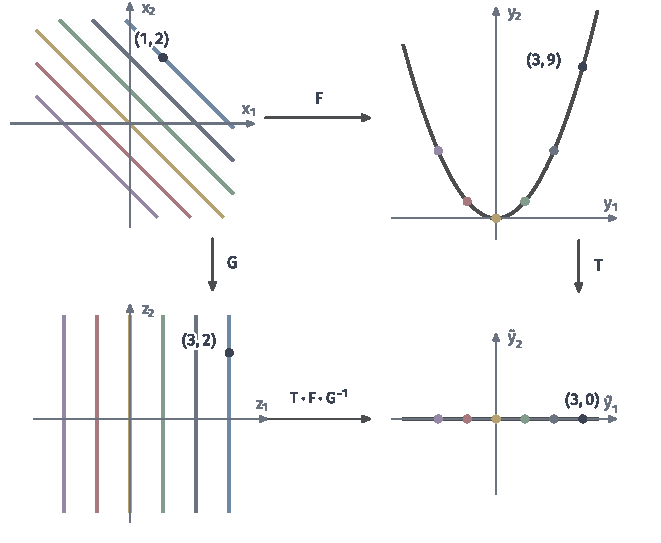
\includegraphics[width=112mm]{figures/04-spaces-measures-and-geometry/04-manifolds/matplotlib/mrel-rank-steps/figure.pdf}
  \caption{常秩定理的三步，$F(x_1,x_2)=(s,s^2)$，$s=x_1+x_2$。左上：源中的等值线$x_1+x_2=c$，$c=-2,\ldots,3$，同一条线上颜色相同。右上：它们被$F$压成抛物线上的一点（同色）。左下：$G$把等值线摆成竖直线。右下：$T$把抛物线压平到坐标轴上。黑点是$(1,2)$的轨迹。}
  \label{fig:mrel-rank-steps}
\end{BookInlineFigure}

\paragraph{浸入与淹没的局部形式}
由上面的满秩讨论，浸入在每点附近秩恒为$m$，淹没恒为$n$，常秩定理直接给出它们的局部形式：
\begin{align}
\text{浸入：}\quad&(x_1,\ldots,x_m)\mapsto(x_1,\ldots,x_m,0,\ldots,0),\label{eq:mrel-immersion-form}\\
\text{淹没：}\quad&(x_1,\ldots,x_n,\ldots,x_m)\mapsto(x_1,\ldots,x_n).\label{eq:mrel-submersion-form}
\end{align}

图~\ref{fig:mrel-normal-forms}画出这两种形式和一般常秩映射。式~\eqref{eq:mrel-immersion-form}说，浸入局部上把$\mathbb R^m$放进$\mathbb R^n$作为前$m$个坐标的子空间，所以局部单射，像的一小块是一片平的$m$维片。式~\eqref{eq:mrel-submersion-form}说，淹没局部上沿后$m-n$个坐标投影，每点的原像局部是一片$m-n$维的片。

\begin{BookInlineFigure}
  \centering
  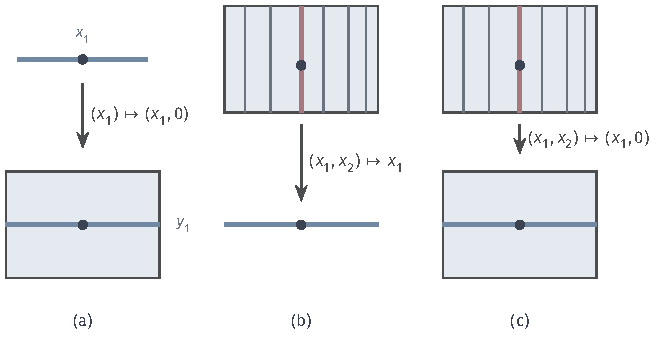
\includegraphics[width=111.767mm]{figures/04-spaces-measures-and-geometry/04-manifolds/tikz/mrel-normal-forms/figure.pdf}
  \caption{常秩映射的局部标准形式。(a)浸入：区间平放进平面，成为一条坐标线。(b)淹没：矩形沿竖直方向投影到区间上，红色竖线是一点的原像。(c)一般的常秩映射（$m=n=2$，$r=1$）：竖线整条压成一点，像是一条横线，定义域和值域都没有被占满。}
  \label{fig:mrel-normal-forms}
\end{BookInlineFigure}

前面的例子都可以写成这样的形式。对$E$，在圆周上用$\mathbb R^2$的极坐标图$(\theta,r-1)$，$E$的坐标表示恰好是$t\mapsto(t,0)$，这就是式~\eqref{eq:mrel-immersion-form}。对高度函数$h$，在$p$附近用坐标$(h,\lambda)$，其中$\lambda$是经度，$h$的坐标表示就是投影$(h,\lambda)\mapsto h$，这就是式~\eqref{eq:mrel-submersion-form}。

表~\ref{tab:mrel-immersion-submersion}把两种映射并排比较。下一节正是用这两种局部形式构造子流形：浸入给出“像”的局部坐标，淹没给出“水平集”的局部坐标。

\begin{BookInlineTable}
  \centering
  \begin{tabular}{lll}
    \toprule
    & 浸入 & 淹没\\
    \midrule
    微分 & 处处单射 & 处处满射\\
    秩 & 恒为$m$ & 恒为$n$\\
    维数 & $m\leq n$ & $m\geq n$\\
    Jacobian矩阵 & 列满秩 & 行满秩\\
    局部形式 & 加上若干零坐标 & 丢掉若干坐标\\
    局部几何 & 像是平的$m$维片 & 原像是平的$(m-n)$维片\\
    \bottomrule
  \end{tabular}
  \caption{浸入与淹没的比较。}
  \label{tab:mrel-immersion-submersion}
\end{BookInlineTable}

\section{嵌入子流形}
\label{sec:mrel-embedded-submanifolds}

浸入在每点附近都像把一块平的片放进目标空间，可这些局部的片拼起来，未必是目标中一个像样的子空间：像可能自己穿过自己，也可能从远处绕回来贴近自身。本节先在浸入之上加入整体的拓扑条件，得到嵌入；再在目标的坐标中描述嵌入子流形的局部样子；最后研究由约束方程定义的集合何时是这样的子流形。

\subsection{嵌入}
\label{sec:mrel-embedding}

\paragraph{“8”字形曲线}
考虑$\alpha:(-\pi,\pi)\to\mathbb R^2$，$\alpha(t)=(\sin2t,\sin t)$。速度$(2\cos2t,\cos t)$处处非零：若$\cos t=0$，则$t=\pm\pi/2$，此时$\cos2t=-1$。所以$\alpha$是浸入。它还是单射：若$\sin t=\sin s$且$t\neq s$，则$s=\pi-t$或$s=-\pi-t$，于是$\sin2s=-\sin2t$，要使第一个分量也相等只能$\sin2t=0$，即$t\in\{0,\pm\pi/2\}$。$t=0$时$s=\pm\pi$不在区间内，$t=\pm\pi/2$时$s=t$，都与假设矛盾。特别地，$t=0$是唯一映到原点的参数。

$\alpha$的像是一个“8”字：$t$从$0$增大到$\pi$时画出一个圈，$t\to\pi$时又回到原点附近；$t$从$0$减小到$-\pi$时画出另一个圈。取$t_k\to\pi$，则$\alpha(t_k)\to(0,0)=\alpha(0)$，但$t_k$不趋于$0$。从像的角度看，点列收敛到原点；从参数的角度看，对应的参数却跑到了区间的另一端。所以$\alpha$作为从$(-\pi,\pi)$到其像的双射，逆映射不连续。

\paragraph{定义}
“8”字形曲线的问题不在局部方向，而在像所继承的拓扑与源流形的拓扑不一致。像$F(M)$作为$N$的子集，有从$N$继承的子空间拓扑：$F(M)$中的开集是$N$中开集与$F(M)$的交。要求$F$在这一拓扑下是同胚，就排除了上述情形。

\begin{definition}[嵌入]
\label{def:mrel-embedding}
光滑映射$F:M\to N$称为\term{嵌入}（embedding），若$F$是浸入，并且$F:M\to F(M)$是同胚，其中$F(M)$带有从$N$继承的子空间拓扑。
\end{definition}

于是有三个层层加强的条件：浸入只要求微分单射；单射浸入还要求映射本身单射；嵌入进一步要求到像的同胚。$E:\mathbb R\to\mathbb R^2$，$t\mapsto(\cos t,\sin t)$是浸入但不是单射，像自己反复重叠；$\alpha$是单射浸入但不是嵌入；把$E$限制到$(0,2\pi)$上，得到单射浸入，它的逆就是角度图$\theta_2$，连续，所以是嵌入。

\paragraph{紧流形的单射浸入}
源流形紧时，后两个条件之间的差距消失。

\begin{theorem}[紧流形上的单射浸入]
\label{thm:mrel-compact-injective-immersion}
若$M$紧，$F:M\to N$是单射浸入，则$F$是嵌入。
\end{theorem}

\begin{proof}
只需证明$F:M\to F(M)$的逆连续，即$F$把$M$的闭集映为$F(M)$的闭集。设$K\subseteq M$是闭集，紧空间的闭子集是紧集，所以$K$紧；连续映射把紧集映为紧集，$F(K)$紧；$N$是Hausdorff空间，其紧子集是闭集，所以$F(K)$在$N$中闭，从而在$F(M)$中闭。
\end{proof}

$\alpha$的源区间$(-\pi,\pi)$不紧，参数可以逃向端点而像却回到原点，定理正是排除了这种逃逸。

\subsection{子流形的局部表示}
\label{sec:mrel-submanifold-local}

\paragraph{切片坐标}
嵌入的像在目标中应当局部像一块平的片。用目标的坐标表达：在合适的图中，像恰好是一部分坐标为零的那片点。

\begin{definition}[嵌入子流形]
\label{def:mrel-embedded-submanifold}
设$M$是$n$维光滑流形，$S\subseteq M$，$0\leq k\leq n$。若对每个$p\in S$，都有$M$的图$(U,\varphi)$，$p\in U$，使
\begin{equation}
\varphi(U\cap S)=\{\bm x\in\varphi(U):x_{k+1}=\cdots=x_n=0\},
\label{eq:mrel-slice-chart}
\end{equation}
则称$S$为$M$的$k$维\term{嵌入子流形}（embedded submanifold）。这样的图称为$S$的\term{切片坐标}（slice chart）。$n-k$称为$S$的\term{余维数}（codimension）。
\end{definition}

切片坐标中的前$k$个坐标在$S$上自由变化，是$S$的内部坐标；后$n-k$个坐标描述离开$S$的方向，在$S$上为零。这一描述与嵌入是同一件事的两面。

\begin{theorem}[嵌入与嵌入子流形]
\label{thm:mrel-embedding-submanifold}
\begin{enumerate}
\item 设$S$是$M$的$k$维嵌入子流形，带子空间拓扑。把切片坐标限制到$U\cap S$并只保留前$k$个坐标，得到$S$的光滑图册，$S$成为$k$维光滑流形，包含映射$\iota:S\to M$是嵌入。
\item 若$F:P\to M$是嵌入，则$F(P)$是$M$的嵌入子流形，维数等于$\dim P$，并且$F:P\to F(P)$是微分同胚。
\end{enumerate}
\end{theorem}

\begin{proof}
第一条。限制后的映射是$U\cap S$到$\mathbb R^k$开集的同胚，因为$\varphi$是同胚，而式\eqref{eq:mrel-slice-chart}说明$U\cap S$恰好对应坐标平面$\mathbb R^k\times\{\bm 0\}$与$\varphi(U)$的交。两张这样的图之间的坐标变换，是$M$的坐标变换限制到$\mathbb R^k\times\{\bm 0\}$上再取前$k$个分量，仍光滑。$S$作为$M$的子空间是Hausdorff且第二可数的。在这些图中，$\iota$的坐标表示是$\bm x'\mapsto(\bm x',\bm 0)$，是浸入；$S$本来就带子空间拓扑，$\iota$到像的同胚是自然的。

第二条。设$p\in P$，$k=\dim P$。$F$是浸入，由常秩定理，有以$p$为中心的图$(U,\varphi)$与以$F(p)$为中心的图$(V,\psi)$，使$\psi\circ F\circ\varphi^{-1}(\bm x')=(\bm x',\bm 0)$。这只说明$F(U)$是一片，还须排除$F(P)$的其他部分从远处进入$V$。这就要用到同胚条件：$F(U)$在$F(P)$中开，所以存在$M$中的开集$W$，使$F(U)=W\cap F(P)$。

令$V'=V\cap W\cap\psi^{-1}\bigl(\varphi(U)\times\mathbb R^{n-k}\bigr)$。若$q\in V'\cap F(P)$，则$q\in W\cap F(P)=F(U)$，所以$\psi(q)=(\bm x',\bm 0)$，$\bm x'\in\varphi(U)$。反过来，若$q\in V'$且$\psi(q)=(\bm x',\bm 0)$，则$\bm x'\in\varphi(U)$，$q=\psi^{-1}(\bm x',\bm 0)=F(\varphi^{-1}(\bm x'))\in F(P)$。所以$\psi$限制到$V'$上是$F(P)$的切片坐标。最后，在$P$的图$\varphi$与$F(P)$的限制图下，$F$的坐标表示是恒等映射，故$F$是到像的微分同胚。
\end{proof}

\paragraph{子流形的切空间}
包含映射$\iota$是浸入，$\mathrm d\iota_p$把$T_pS$单射地送入$T_pM$。今后把$T_pS$与它的像$\mathrm d\iota_p(T_pS)$等同，看作$T_pM$的$k$维子空间。在切片坐标中，$\iota$的坐标表示是$\bm x'\mapsto(\bm x',\bm 0)$，所以
\[
T_pS=\operatorname{span}\bigl\{\partial_1|_p,\ldots,\partial_k|_p\bigr\}\subseteq T_pM .
\]
沿后$n-k$条坐标线运动会离开$S$，相应的方向不在$T_pS$中。当$M=\mathbb R^n$时，$T_pM$就是$\mathbb R^n$，$T_pS$成为$\mathbb R^n$的一个线性子空间，这就是嵌入在欧氏空间中的曲线与曲面的切向量的通常含义。

\paragraph{例子：圆周、球面、图像与乘积}
圆周$S^1\subseteq\mathbb R^2$。在去掉负半轴$\{(y_1,0):y_1\leq0\}$的平面上用极坐标$(\theta,r)$，令$\varphi(\bm y)=(\theta,r-1)$。在这张图中，$S^1$恰好对应第二个坐标为零，所以它是切片坐标；另一张图用去掉正半轴的极坐标。于是$S^1$是$\mathbb R^2$的一维嵌入子流形，余维数为$1$。三种坐标在这里分得很清楚：$\theta$是圆周的内部坐标，$(y_1,y_2)$是环境坐标，$r-1$是只在环境中有意义的离开圆周的坐标。球面$S^2\subseteq\mathbb R^3$用球坐标$(\theta,\phi,r-1)$类似处理。

光滑函数$f:W\to\mathbb R^{n-k}$（$W\subseteq\mathbb R^k$开）的图像$\Gamma_f=\{(\bm x,f(\bm x)):\bm x\in W\}$是$W\times\mathbb R^{n-k}$的嵌入子流形：$\varphi(\bm x,\bm y)=(\bm x,\bm y-f(\bm x))$是微分同胚，逆为$(\bm x,\bm z)\mapsto(\bm x,\bm z+f(\bm x))$，它把$\Gamma_f$送到$\{\bm z=\bm0\}$。这个例子说明，局部上“是图像”与“有切片坐标”是一回事，下一小节的隐函数表示正是把子流形局部写成图像。

乘积也保持子流形关系。若$S_1\subseteq M_1$与$S_2\subseteq M_2$分别是嵌入子流形，两张切片坐标的乘积是$S_1\times S_2$在$M_1\times M_2$中的切片坐标，只需把坐标重新排序，使取零的坐标放在最后。例如环面$S^1\times S^1$是$\mathbb R^2\times\mathbb R^2=\mathbb R^4$的二维嵌入子流形，余维数为$2$。

\paragraph{不是子流形的子集}
子流形的定义对每个点都要求切片坐标，任意子集未必满足。十字形$X=\{(y_1,y_2):y_1y_2=0\}$在原点以外是两条坐标轴，局部是直线；但在原点处，它不是一维子流形。若是，原点在$X$中有一个连通邻域同胚于开区间，去掉原点后恰有两个连通分支；可原点在$X$中的任何足够小的连通邻域，去掉原点后都有四个分支，即四条半轴的片段。“8”字形曲线的像在原点处也是同样的十字形交叉，所以$\alpha$的像不是嵌入子流形，与$\alpha$不是嵌入相符。

还有更隐蔽的情形。尖点曲线$\{y_2^2=y_1^3\}$作为拓扑空间同胚于实轴，没有十字交叉，但可以证明它在原点处没有切片坐标，因而不是$\mathbb R^2$的光滑嵌入子流形，这里不给出证明。上一节的参数化$\beta(t)=(t^2,t^3)$恰好在原点速度为零，与此相呼应。可见判断是否为子流形，既要看拓扑，也要看光滑结构。

\subsection{正则水平集}
\label{sec:mrel-regular-level-sets}

很多子流形由约束方程给出：球面是$\lVert\bm y\rVert_2^2=1$的解集，正交矩阵是$\bm A^\top\bm A=\bm I$的解集。问题是：约束方程的解集何时是子流形，维数是多少，切空间是什么？

\paragraph{正则值}
设$\Phi:M\to N$光滑，$c\in N$。水平集$\Phi^{-1}(c)$由所有满足约束$\Phi(p)=c$的点组成。若每个约束都提供一个独立的方向限制，就应当把$m$个自由度减去$n$个。“独立”的准确含义是微分满秩。

\begin{definition}[正则值与正则水平集]
\label{def:mrel-regular-value}
设$\Phi:M\to N$光滑。若$\mathrm d\Phi_p$是满射，称$p$为$\Phi$的正则点，否则称为临界点。若$\Phi^{-1}(c)$中的每一点都是正则点，称$c$为$\Phi$的\term{正则值}（regular value），$\Phi^{-1}(c)$称为\term{正则水平集}（regular level set）。
\end{definition}

按定义，不在像中的点也是正则值，这时水平集为空，下面的定理对空集自然成立。

\begin{theorem}[正则水平集定理]
\label{thm:mrel-regular-level-set}
设$\Phi:M\to N$光滑，$c$是$\Phi$的正则值。则$S=\Phi^{-1}(c)$是$M$的$m-n$维嵌入子流形，并且对每个$p\in S$，
\[
T_pS=\ker\mathrm d\Phi_p .
\]
\end{theorem}

\begin{proof}
正则点组成的集合$M_0$是开集，因为满秩在附近保持。$S\subseteq M_0$，$\Phi$在$M_0$上是淹没，由常秩定理，每个$p\in S$附近有图$\varphi$与以$c$为中心的图$\psi$，使$\psi\circ\Phi\circ\varphi^{-1}(x_1,\ldots,x_m)=(x_1,\ldots,x_n)$。于是$S$在这张图中恰好是$x_1=\cdots=x_n=0$的点。把坐标重新排序，让这$n$个坐标排在最后，就得到$m-n$维的切片坐标。

$\Phi$在$S$上取常值$c$，所以$\Phi\circ\iota$是常值映射，微分为零，即$\mathrm d\Phi_p\circ\mathrm d\iota_p=0$，$T_pS\subseteq\ker\mathrm d\Phi_p$。$\mathrm d\Phi_p$满射，由秩--零度关系，核的维数是$m-n$，与$T_pS$相同，所以二者相等。
\end{proof}

定理与隐函数定理是同一件事的两种说法。在欧氏情形，$\Phi:\mathbb R^m\to\mathbb R^n$在$p$处的Jacobian矩阵行满秩，可以选出$n$列组成可逆方阵；隐函数定理把对应的$n$个变量解成其余$m-n$个变量的光滑函数，水平集在$p$附近就是这个函数的图像，再由上一小节的图像例子得到切片坐标。满秩条件排除了局部奇点：在不满秩的点，约束之间可能互相重复，也可能在该点退化，解集在那里可以出现交叉或孤立点。

\paragraph{球面}
令$\Phi:\mathbb R^3\to\mathbb R$，$\Phi(\bm y)=\lVert\bm y\rVert_2^2$。$\mathrm d\Phi_{\bm y}(\bm v)=2\bm y^\top\bm v$，当$\bm y\neq\bm 0$时它是到$\mathbb R$的满射。$\Phi^{-1}(1)=S^2$不含原点，所以$1$是正则值，$S^2$是二维嵌入子流形，并且
\[
T_{\bm p}S^2=\{\bm v\in\mathbb R^3:\bm p^\top\bm v=0\},
\]
即与$\bm p$正交的平面。这与第~\ref{chap:manifold-basics}章用球极投影算出的切向量$(0.2,0,0)$与$\bm p=(0,\tfrac35,\tfrac45)$正交一致。同样，椭球面是$\sum_iy_i^2/a_i^2=1$的正则水平集；线性映射$\bm y\mapsto(y_1/a_1,y_2/a_2,y_3/a_3)$把它一一映到球面，在两侧的子流形结构下是微分同胚，这就是本章开头说椭球面与球面“本质上相同”的含义。

\paragraph{正则性只是充分条件}
不满足正则性时，水平集可能不是子流形。$\Phi(y_1,y_2)=y_1^2-y_2^2$在原点处微分为零，$\Phi^{-1}(0)$是两条直线$y_2=\pm y_1$的并，在原点处交叉，与上一小节的十字形一样不是子流形。$\Phi(\bm y)=\lVert\bm y\rVert_2^2$的零水平集只有原点，是零维子流形，却不是定理预测的二维；那里原点是临界点，定理本来就不适用。

水平集也可能在正则性失败时仍是子流形。$\Phi(\bm y)=(\lVert\bm y\rVert_2^2-1)^2$的零水平集仍是单位圆，但在圆上$\mathrm d\Phi=4(\lVert\bm y\rVert_2^2-1)\bm y^\top=\bm 0$，没有一个点是正则点。这说明正则值是水平集为子流形的充分条件，不是必要条件；同一个集合换一个约束函数，正则性可能成立，也可能不成立。

\paragraph{正交矩阵与重复方程}
全体$n$阶正交矩阵组成的集合$\mathrm O(n)=\{\bm A\in\mathbb R^{n\times n}:\bm A^\top\bm A=\bm I\}$称为\term{正交群}（orthogonal group）。它由$n^2$个方程定义，但这些方程有重复：$\bm A^\top\bm A$总是对称矩阵，第$(i,j)$个方程与第$(j,i)$个方程相同。若把约束映射看成取值于$\mathbb R^{n\times n}$，它的微分只能取到对称矩阵，永远不是满射，单位矩阵不是正则值，定理用不上。

正确的做法是让约束映射取值于对称矩阵组成的空间$\operatorname{Sym}(n)$，它是$n(n+1)/2$维线性空间。令$\Phi:\mathbb R^{n\times n}\to\operatorname{Sym}(n)$，$\Phi(\bm A)=\bm A^\top\bm A$。对方向$\bm H$求导，
\[
\mathrm d\Phi_{\bm A}(\bm H)=\bm H^\top\bm A+\bm A^\top\bm H .
\]
在$\bm A\in\mathrm O(n)$处，任给对称矩阵$\bm C$，取$\bm H=\tfrac12\bm A\bm C$，利用$\bm A^\top\bm A=\bm I$与$\bm C^\top=\bm C$，得
\[
\mathrm d\Phi_{\bm A}\bigl(\tfrac12\bm A\bm C\bigr)=\tfrac12\bm C^\top\bm A^\top\bm A+\tfrac12\bm A^\top\bm A\bm C=\bm C .
\]
所以$\mathrm d\Phi_{\bm A}$是满射，$\bm I$是正则值。

由定理~\ref{thm:mrel-regular-level-set}，$\mathrm O(n)$是$\mathbb R^{n\times n}$的嵌入子流形，维数为$n^2-n(n+1)/2=n(n-1)/2$。在单位矩阵处，$T_{\bm I}\mathrm O(n)=\ker\mathrm d\Phi_{\bm I}=\{\bm H:\bm H^\top+\bm H=\bm 0\}$，即全体反对称矩阵，维数恰为$n(n-1)/2$，与上面一致。$n=2$时维数为$1$，对应平面旋转的一个转角参数；$n=3$时维数为$3$，对应三维旋转的三个自由度。$\mathrm O(n)$既是流形又是群，这种结构在第~\ref{chap:lie-groups}章研究。

\paragraph{带边界的情形}
本章的结论都针对无边界流形。约束若是不等式，例如闭球$\{\bm y:\lVert\bm y\rVert_2^2\leq1\}$，所得集合是带边界流形，边界恰是正则水平集$\{\lVert\bm y\rVert_2^2=1\}$。一般地，若$c$是光滑实值函数$\Phi:M\to\mathbb R$的正则值，下水平集$\{\Phi\leq c\}$是与$M$同维的带边界流形，边界为$\Phi^{-1}(c)$；证明要在边界点处单独构造半空间坐标，这里不给出。约束集合本身带边界，或映射的定义域带边界时，上述定理都需要另核条件。

\section{本章小结}
\label{sec:mrel-summary}

本章开头问了两个问题：两个流形何时在光滑意义下相同，一个对象何时是另一个流形中的光滑子集。第一个问题由微分同胚回答。它是光滑且逆光滑的双射，比同胚多保留了光滑结构，比集合双射多保留了拓扑；$x\mapsto x^3$是光滑的同胚，却不是微分同胚。

微分同胚在每点的微分都是线性同构，所以维数相同。反过来，反函数定理只说明微分在一点可逆时映射在该点附近是微分同胚。$E(t)=(\cos t,\sin t)$与圆周的倍角映射都是局部微分同胚，却不是单射，整体的双射性必须另外核对。微分同胚也不保持长度，$(0,1)$与$\mathbb R$微分同胚。

映射的局部结构由微分的秩决定。浸入的微分处处单射，淹没的微分处处满射，它们分别要求源的维数不超过或不小于目标的维数，并且与映射本身是否单射、满射无关。一点的秩只给出附近秩的下限，$x\mapsto x^2$在原点秩为零、附近秩为一，没有局部标准形式。

在秩保持不变的邻域中，常秩定理用反函数定理把映射化为“前$r$个坐标不变、其余坐标为零”的标准形式。满秩是开条件，所以浸入与淹没自动满足常秩条件，分别局部像坐标子空间的包含与坐标投影。

第二个问题需要整体条件。“8”字形曲线是单射浸入，参数却可以逃向端点而像回到原点，它到像的逆不连续；环面上的无理斜率直线则处处如此。嵌入在浸入之上要求到像的同胚，紧流形上的单射浸入自动是嵌入。

嵌入的像正是嵌入子流形，即每点附近有切片坐标、子流形对应一部分坐标为零的集合；切空间是前几个坐标基向量张成的子空间。圆周、球面、函数图像与乘积都有切片坐标，十字形和“8”字的交叉点则没有，尖点虽然拓扑上是直线，也没有切片坐标。

约束方程提供了构造子流形的一般办法。若$c$是$\Phi:M\to N$的正则值，水平集$\Phi^{-1}(c)$是$m-n$维嵌入子流形，切空间是$\ker\mathrm d\Phi_p$。球面与椭球面由此得到；正交群$\mathrm O(n)$也由此得到，但约束映射要取值于对称矩阵空间，以免把重复的方程计入满秩要求，所得维数为$n(n-1)/2$，单位元处的切空间是反对称矩阵。正则值只是充分条件，$(\lVert\bm y\rVert_2^2-1)^2$的零水平集是圆，却没有正则点。

本章始终在无边界情形下讨论，带边界时反函数定理与正则水平集定理都要另核条件。所有结论都只涉及光滑结构，不涉及长度和角度。在第~\ref{chap:riemannian-geometry}章给切空间配上内积之后，才能问一个微分同胚是否保持长度，即两个黎曼流形是否等距。


\chapter{黎曼几何}
\label{chap:riemannian-geometry}

在地球表面上，北京到纽约有多远？航线给出的数字是沿地面量出的路程，而不是穿过地球内部的直线距离。两地的风向都叫“向东”，可它们分别画在两个不同的切平面里，作为三维向量相减并不为零。这两件小事指向同一个缺口：光滑流形告诉我们哪些曲线光滑、每点有哪些切方向，却没有说一条曲线有多长，也没有说两个不同点处的方向该怎样比较。

第~\ref{chap:manifold-basics}章的球面点$p=(0,\tfrac35,\tfrac45)$上有一个切向量，它在北极图中的分量是$(1,0)$，在南极图中的分量是$(\tfrac19,0)$。这两个数组一样都不能回答“它有多长”，因为$(1,0)$的长度为$1$只是坐标里的说法。放进$\mathbb R^3$之后它是$(\tfrac15,0,0)$，长度是$\tfrac15$。本章要把这种读取长度的能力变成流形自身的一项结构，并用同一个球面把后面的计算走一遍。

本章在同一个光滑流形上依次补上这些结构。第~\ref{sec:riem-metric}节在每个切空间放一个随位置光滑变化的内积，第~\ref{sec:riem-length-distance}节由它累计曲线长度，再对连接两点的全部曲线取下确界，得到内在距离。比较不同点的切向量需要另一项规定：第~\ref{sec:riem-connections}节的联络说明怎样沿一个方向对向量场求导，第~\ref{sec:riem-parallel-transport}节沿曲线令这一导数为零，得到搬运切向量的规则。

速度沿自身平行移动的曲线是测地线。第~\ref{sec:riem-geodesic-ivp}节由初始位置和速度求测地线，并用指数映射汇总这些轨迹；第~\ref{sec:riem-shortest-paths}节转向固定两个端点的问题，判断测地线何时真正最短、最短路线何时存在。第~\ref{sec:riem-curvature}节用协变导数的次序差定义曲率，说明平行移动为何依赖路径，并把内在曲率与曲面在环境中的弯曲区分开。最后，第~\ref{sec:riem-isometries}节用等距映射比较两个黎曼流形。

本章以无边界流形为主，沿用第~\ref{chap:manifold-basics}章的切空间、向量场与Lie括号，第~\ref{chap:manifold-maps}章的微分$\mathrm dF_p$，第~\ref{chap:manifold-relations}章的嵌入子流形。平行移动和测地线依赖常微分方程初值问题的存在唯一性，所用结论就地陈述，证明归入卷六。体积、梯度、散度和Laplace--Beltrami算子在第~\ref{chap:manifold-calculus}章建立；Lie群上的矩阵指数在第~\ref{chap:lie-groups}章讨论，它与本章的指数映射来源不同。

\section{黎曼度量}
\label{sec:riem-metric}

切空间$T_pM$是线性空间，可以把切向量相加、数乘，却还不能回答“这个速度有多快”“这两个方向是否垂直”。欧氏空间中这两个问题由内积回答，流形上自然的做法是给每个切空间各配一个内积。困难在于不同点的切空间是不同的线性空间，内积必须逐点指定；为了能对长度求积分、对内积求导，还要求它随位置光滑变化。

\paragraph{度量的定义}
设$M$是$n$维光滑流形。在坐标图$(U,\varphi)$中记坐标为$x=(x^1,\ldots,x^n)$，上标是坐标编号而不是幂；相应的坐标切基记为$\partial_1,\ldots,\partial_n$，它们在每点$p\in U$构成$T_pM$的基（第~\ref{chap:manifold-basics}章）。切向量$u\in T_pM$写成$u=\sum_iu^i\partial_i$，数组$(u^1,\ldots,u^n)$是它在这组基下的分量。

\begin{definition}[黎曼度量]
\label{def:riem-metric}
光滑流形$M$上的\term{黎曼度量}（Riemannian metric）$g$为每个点$p\in M$指定切空间上的一个内积
\[
g_p:T_pM\times T_pM\to\mathbb R,
\]
即对称、双线性且正定的函数，并且满足光滑性：在任一坐标图中，函数$g_{i,j}(x)=g_p(\partial_i,\partial_j)$（$p=\varphi^{-1}(x)$）都是$x$的光滑函数。带有黎曼度量的光滑流形$(M,g)$称为\term{黎曼流形}（Riemannian manifold）。
\end{definition}

定义里的三项要求各有分工。对称与双线性使$g_p$由矩阵$\bm G(x)=[g_{i,j}(x)]$完全确定：若$u,v$的分量为$(u^i)$与$(v^j)$，则
\begin{equation}
g_p(u,v)=\sum_{i,j=1}^n g_{i,j}(x)\,u^iv^j .
\label{eq:riem-metric-coordinates}
\end{equation}
正定性要求$\bm G(x)$对称正定，于是长度$\lVert u\rVert_g=\sqrt{g_p(u,u)}$只在$u=0$时为零，非零向量的夹角$\vartheta$由$\cos\vartheta=g_p(u,v)/(\lVert u\rVert_g\lVert v\rVert_g)$确定。光滑性则把逐点的内积连成一个整体对象；后面求联络系数时要对$g_{i,j}$求导，这一条件不可省。

光滑性条件中的“任一坐标图”并不需要逐张核对。换用另一组坐标$y$时，记$\bm A(y)=[\partial x^i/\partial y^a]$为坐标变换的Jacobian矩阵。同一个切向量的旧分量等于$\bm A$乘新分量，代入式\eqref{eq:riem-metric-coordinates}得到
\begin{equation}
\widetilde{\bm G}(y)=\bm A(y)^{\top}\bm G(x(y))\bm A(y).
\label{eq:riem-metric-transform}
\end{equation}
右端各因子都光滑，所以一张图中光滑，重叠处的另一张图中也光滑。这个变换规律也说明，$\bm G$的条目本身随坐标改变，不变的是它所规定的内积。

\paragraph{同一几何的不同坐标}
欧氏平面取标准内积。直角坐标中$\bm G=\bm I$；改用极坐标$(r,\theta)$，$r>0$，坐标切基为$\partial_r=(\cos\theta,\sin\theta)^{\top}$与$\partial_\theta=(-r\sin\theta,r\cos\theta)^{\top}$，于是
\[
\bm G(r,\theta)=\begin{bmatrix}1&0\\0&r^2\end{bmatrix}.
\]
系数随位置变化，并不说明几何改变了：$\partial_\theta$表示“角度增加一单位”的运动，在半径$r$处走过的弧长约为$r$。度量矩阵记录的是坐标单位与真实长度之间的换算，同一几何在不同坐标中可以有不同的矩阵。

\paragraph{嵌入诱导的度量}
曲面通常坐落在欧氏空间中，此时最自然的长度就是环境中的长度。设$M\subseteq\mathbb R^D$是嵌入子流形（第~\ref{chap:manifold-relations}章），局部参数化$\Phi:V\to M$的Jacobian矩阵$\bm J(x)=[\partial\Phi/\partial x^1,\ldots,\partial\Phi/\partial x^n]$满列秩，它的各列正是坐标切向量在$\mathbb R^D$中的表示。把环境内积限制到切空间，得到
\begin{equation}
\bm G(x)=\bm J(x)^{\top}\bm J(x),\qquad g_{i,j}=\Bigl\langle\frac{\partial\Phi}{\partial x^i},\frac{\partial\Phi}{\partial x^j}\Bigr\rangle .
\label{eq:riem-induced-metric}
\end{equation}
满列秩保证$\bm a^{\top}\bm G\bm a=\lVert\bm J\bm a\rVert_2^2>0$对非零$\bm a\in\mathbb R^n$成立，所以$\bm G$正定。这样得到的度量称为\term{诱导度量}（induced metric）。若参数化在某点秩亏，同一公式只给出半正定矩阵，不再满足黎曼度量的定义。

\begin{example}[单位球面的诱导度量]
\label{ex:riem-sphere-metric}
单位球面$\mathbb S^2\subseteq\mathbb R^3$在去掉两极和一条经线后，可用极角$\theta\in(0,\pi)$与方位角$\phi\in(0,2\pi)$参数化：
\[
\Phi(\theta,\phi)=(\sin\theta\cos\phi,\ \sin\theta\sin\phi,\ \cos\theta)^{\top}.
\]
两列切向量为$\partial_\theta\Phi=(\cos\theta\cos\phi,\cos\theta\sin\phi,-\sin\theta)^{\top}$与$\partial_\phi\Phi=(-\sin\theta\sin\phi,\sin\theta\cos\phi,0)^{\top}$，二者内积为零，长度平方分别为$1$与$\sin^2\theta$，所以
\[
\bm G(\theta,\phi)=\begin{bmatrix}1&0\\0&\sin^2\theta\end{bmatrix}.
\]
沿纬线（固定$\theta$）方位角增加$\Delta\phi$，走过的长度是$\sin\theta\,\Delta\phi$：越靠近两极，同样的角度变化对应越短的路程。
\end{example}

\paragraph{同一流形上的不同度量}
诱导度量只是一种选择。同一个光滑流形可以配上许多不同的黎曼度量，它们给出不同的长度和角度。例如在上半平面$H=\{(x,y):y>0\}$上，除了欧氏度量$\bm G=\bm I$，还可以取
\[
\bm G(x,y)=\frac1{y^2}\begin{bmatrix}1&0\\0&1\end{bmatrix}.
\]
两者在每点只差一个正的倍数，所以角度相同；长度却不同：在这种度量下，竖直线段从$y=1$走到$y=\varepsilon$的长度是$\int_\varepsilon^1 y^{-1}\,\mathrm dy=\ln(1/\varepsilon)$，当$\varepsilon\to0$时趋于无穷，而欧氏长度不超过$1$。下一节的距离、第~\ref{chap:manifold-calculus}章的体积和梯度都由度量决定，所以凡是谈论这些量，都要说明所用的是哪一个度量。

\paragraph{度量的存在}
一般光滑流形不一定嵌在给定的欧氏空间中，但总存在黎曼度量。取一族坐标图$\{(U_\alpha,\varphi_\alpha)\}$和从属于它的光滑单位分解$\{\psi_\alpha\}$（第~\ref{chap:manifold-basics}章），在每张图中先用坐标的欧氏内积定义$g^{(\alpha)}$，再令
\[
g_p(u,v)=\sum_\alpha\psi_\alpha(p)\,g^{(\alpha)}_p(u,v).
\]
$\psi_\alpha$的支撑含于$U_\alpha$，所以每一项在$U_\alpha$外按零延拓后仍光滑；每点附近只有有限项非零，所以和是光滑的；对称与双线性逐项保持。对非零$u$，每项$\psi_\alpha(p)g^{(\alpha)}_p(u,u)\geq0$，且至少有一个$\psi_\alpha(p)>0$，相应一项严格为正，故$g_p$正定。这个构造依赖的是正定矩阵的非负组合仍正定；它只说明度量存在，并不挑出某个“正确”的度量。

\section{曲线长度与内在距离}
\label{sec:riem-length-distance}

有了每个切空间中的长度，就可以把一条曲线各时刻的速率累计起来，得到曲线的长度。两点之间的距离则不是某一条曲线的属性，而要比较所有连接这两点的曲线。本节先定义长度并检查它与参数化无关，再用下确界定义内在距离，最后把它与环境空间中的直线距离比较。

\paragraph{曲线长度}
实际路线常有拐角，例如沿两段大圆弧拼成的航线。因此考虑\emph{分段光滑曲线}$\gamma:[a,b]\to M$：它连续，并且存在分点$a=t_0<t_1<\cdots<t_m=b$，使$\gamma$在每个$[t_{r-1},t_r]$上光滑。除有限个分点外，速度$\dot\gamma(t)\in T_{\gamma(t)}M$都有定义（第~\ref{chap:manifold-basics}章）。

\begin{definition}[曲线长度]
\label{def:riem-curve-length}
黎曼流形$(M,g)$上分段光滑曲线$\gamma:[a,b]\to M$的\term{曲线长度}（length of a curve）为
\begin{equation}
L_g(\gamma)=\int_a^b\lVert\dot\gamma(t)\rVert_g\,\mathrm dt
=\int_a^b\sqrt{g_{\gamma(t)}\bigl(\dot\gamma(t),\dot\gamma(t)\bigr)}\,\mathrm dt .
\label{eq:riem-curve-length}
\end{equation}
\end{definition}

若曲线落在一张坐标图内，写成坐标曲线$x(t)$，则被积函数是
\begin{equation*}
\sqrt{\sum_{i,j}g_{i,j}(x(t))\dot x^i(t)\dot x^j(t)}.
\end{equation*}
曲线跨越多张图时，紧区间$[a,b]$可以分成有限段，使每段落在一张图内；这一点来自$\gamma([a,b])$的紧性。式\eqref{eq:riem-metric-transform}保证在重叠处换图后被积函数不变，所以分段方式不影响结果。

\begin{example}[球面纬线的长度]
\label{ex:riem-latitude-length}
在例~\ref{ex:riem-sphere-metric}的坐标中取纬线$\gamma(t)=\Phi(\theta_0,t)$，$t\in[0,2\pi]$，严格说这条闭曲线有一点落在所取坐标域外，但单点不影响积分。坐标速度为$(\dot\theta,\dot\phi)=(0,1)$，于是$\lVert\dot\gamma\rVert_g^2=\sin^2\theta_0$，长度为$2\pi\sin\theta_0$。赤道$\theta_0=\pi/2$给出$2\pi$，靠近北极的纬线长度趋于零，与三维中圆的周长$2\pi\times(\text{半径}\sin\theta_0)$一致。
\end{example}

长度应当是路线本身的属性，不应取决于沿路线走得快还是慢。下面的结论说明定义满足这一要求。

\begin{theorem}[长度与参数化无关]
\label{thm:riem-length-reparametrization}
设$\gamma:[a,b]\to M$分段光滑，$\tau:[c,d]\to[a,b]$是分段光滑的单调满射，且$\tau'$除有限点外有定义并保持符号不变。则$L_g(\gamma\circ\tau)=L_g(\gamma)$。
\end{theorem}

\begin{proof}
由链式法则，$(\gamma\circ\tau)^{\cdot}(s)=\tau'(s)\dot\gamma(\tau(s))$，所以$\lVert(\gamma\circ\tau)^{\cdot}(s)\rVert_g=\lvert\tau'(s)\rvert\,\lVert\dot\gamma(\tau(s))\rVert_g$。若$\tau'\geq0$，作换元$t=\tau(s)$，$\mathrm dt=\tau'(s)\mathrm ds$，即得$\int_c^d\lVert\dot\gamma(\tau(s))\rVert_g\tau'(s)\,\mathrm ds=\int_a^b\lVert\dot\gamma(t)\rVert_g\,\mathrm dt$。若$\tau'\leq0$，换元后积分上下限互换，绝对值恰好抵消这一符号。分段光滑的情形逐段应用这一论证。
\end{proof}

定理要求$\tau$单调。若参数来回走，例如先前进再后退再前进，经过的路线被重复计入，长度会增加；这不是“换速度”，而是换了一条路线。

\paragraph{内在距离}
长度评价给定的一条路线，距离则要在所有允许路线中取最好的一条。这里“允许”指始终留在$M$中：穿过地球内部的直线不是地面上的路线。若两点之间所有路线的长度没有最小值，仍可以取下确界。

\begin{definition}[内在距离]
\label{def:riem-intrinsic-distance}
设$(M,g)$是黎曼流形，$p,q$属于$M$的同一个连通分支。定义$p,q$之间的\term{内在距离}（intrinsic distance）为
\begin{equation}
d_g(p,q)=\inf\bigl\{L_g(\gamma):\gamma:[a,b]\to M\text{分段光滑},\ \gamma(a)=p,\ \gamma(b)=q\bigr\}.
\label{eq:riem-intrinsic-distance}
\end{equation}
它也常称为测地距离。若$p,q$位于不同连通分支，约定$d_g(p,q)=+\infty$。
\end{definition}

这个集合非空，需要先有连接两点的分段光滑曲线。第~\ref{chap:manifold-basics}章证明连通流形是路径连通的，所用的路径在每个坐标球内由线段拼成，正是分段光滑曲线。因此在同一连通分支内，下确界是对非空集合取的，结果是有限非负数。

\begin{theorem}[内在距离是度量]
\label{thm:riem-distance-metric}
在黎曼流形$(M,g)$的每个连通分支上，$d_g$满足度量的三条公理：$d_g(p,q)\geq0$且仅当$p=q$时为零；$d_g(p,q)=d_g(q,p)$；$d_g(p,r)\leq d_g(p,q)+d_g(q,r)$。
\end{theorem}

\begin{proof}
对称性来自把曲线倒过来走：$t\mapsto\gamma(a+b-t)$连接$q$到$p$，由定理~\ref{thm:riem-length-reparametrization}长度不变。对三角不等式，任给$\varepsilon>0$，取连接$p,q$的曲线$\gamma_1$与连接$q,r$的曲线$\gamma_2$，使$L_g(\gamma_1)<d_g(p,q)+\varepsilon$，$L_g(\gamma_2)<d_g(q,r)+\varepsilon$。首尾相接得到连接$p,r$的分段光滑曲线，长度为两者之和，所以$d_g(p,r)<d_g(p,q)+d_g(q,r)+2\varepsilon$；令$\varepsilon\to0$即可。

剩下的是$p\neq q$时$d_g(p,q)>0$。取$p$附近的坐标图，使$p$的坐标为$x_p$，并取半径$\rho>0$的闭坐标球$\bar B=\{x:\lVert x-x_p\rVert_2\leq\rho\}$落在图内且不含$q$；这一步用到流形的Hausdorff性。$\bm G(x)$的最小特征值在紧集$\bar B$上连续且为正，因此有下界$\lambda>0$，使$\sum_{i,j}g_{i,j}(x)\xi^i\xi^j\geq\lambda\lVert\xi\rVert_2^2$对$x\in\bar B$成立。

任何从$p$到$q$的曲线都要离开$\bar B$，记它的坐标第一次到达球面$\lVert x-x_p\rVert_2=\rho$的时刻为$t^\ast$。在$[a,t^\ast]$上曲线留在$\bar B$中，所以
\[
L_g(\gamma)\geq\int_a^{t^\ast}\sqrt\lambda\,\lVert\dot x(t)\rVert_2\,\mathrm dt\geq\sqrt\lambda\,\bigl\lVert x(t^\ast)-x_p\bigr\rVert_2=\sqrt\lambda\,\rho .
\]
第二个不等式是“坐标曲线的欧氏长度不小于端点距离”。下界与曲线无关，所以$d_g(p,q)\geq\sqrt\lambda\,\rho>0$。
\end{proof}

于是每个连通分支$(M,d_g)$都是第~\ref{chap:metric-spaces}章意义下的度量空间，完备性、Cauchy列等概念都可以使用。若在闭坐标球上再取最大特征值的上界$\Lambda$，类似的估计给出$d_g$与坐标欧氏距离在局部互相控制，由此可以证明$d_g$诱导的拓扑恰为流形原有的拓扑。这里不给出完整证明；后文用到的只是这一结论：$d_g$意义下的收敛与流形拓扑中的收敛是同一回事。

\paragraph{内在距离与环境距离}
对嵌入$\mathbb R^D$并取诱导度量的流形，现在有两种距离：环境中的欧氏距离$\lVert q-p\rVert_2$，以及只允许沿$M$走的内在距离$d_g(p,q)$。二者总有确定的大小关系。对连接$p,q$的任一分段光滑曲线，把它看成$\mathbb R^D$中的曲线，由微积分基本定理与积分的三角不等式，
\[
\lVert q-p\rVert_2=\Bigl\lVert\int_a^b\dot\gamma(t)\,\mathrm dt\Bigr\rVert_2\leq\int_a^b\lVert\dot\gamma(t)\rVert_2\,\mathrm dt=L_g(\gamma),
\]
其中最后一步用的是诱导度量下$\lVert\dot\gamma\rVert_g=\lVert\dot\gamma\rVert_2$。对所有曲线取下确界，得到$\lVert q-p\rVert_2\leq d_g(p,q)$。

单位圆给出最简单的比较。圆心角为$\theta\in[0,\pi]$的两点之间，弦长是$2\sin(\theta/2)$，沿圆周的短弧长度是$\theta$，而任何连接这两点的圆上曲线都至少要扫过这段角度，所以$d_g=\theta$。$\theta=\pi/2$时两者分别约为$1.414$与$1.571$。展开$2\sin(\theta/2)=\theta-\theta^3/24+O(\theta^5)$可见，近处两种距离只差三阶小量，远处差别明显；对跖点之间弦长为$2$，内在距离为$\pi$。

\paragraph{下确界未必达到}
定义使用下确界而不是最小值，是因为最短路线可能不存在。在穿孔平面$M=\mathbb R^2\setminus\{0\}$上取欧氏度量，连接$p=(-1,0)$与$q=(1,0)$。沿横轴走到$(-\varepsilon,0)$，绕半径$\varepsilon$的上半圆到$(\varepsilon,0)$，再沿横轴到$q$，长度为
\[
(1-\varepsilon)+\pi\varepsilon+(1-\varepsilon)=2+(\pi-2)\varepsilon .
\]
令$\varepsilon\to0$，并结合上一段的下界$d_g(p,q)\geq\lVert q-p\rVert_2=2$，得到$d_g(p,q)=2$。长度恰为$2$的连接曲线只能是线段本身（可以改变速度），而线段经过被删去的原点，所以没有任何允许曲线达到下确界。

这个例子区分了两件事：两点之间存在连接曲线，只保证$d_g$有限；存在一条长度恰为$d_g$的曲线，是更强的要求。穿孔平面连通，第一件事成立，第二件事失败。最短曲线何时存在，要在第~\ref{sec:riem-shortest-paths}节借助完备性回答。

\section{联络}
\label{sec:riem-connections}

度量在每个切空间内部比较向量，却不能比较两个不同点处的向量。单位圆上，$p=(1,0)$处的切向量$u=(0,1)$与$q=(0,1)$处的切向量$w=(-1,0)$都表示“逆时针前进一单位”，直觉上方向相同；可是作为$\mathbb R^2$中的向量，$u-w=(1,1)\neq0$，而且$u$根本不在$T_q\mathbb S^1$中。一般流形甚至没有环境空间可供相减。要谈“向量场沿某个方向变化了多少”，就必须规定怎样对向量场求导。

这项规定称为联络。它不是光滑结构自带的，同一个流形上可以有许多联络；有了黎曼度量之后，再加上两条自然的要求，就能从中唯一地选出一个。本节先给出联络的一般定义及其坐标计算，再确定后文一直使用的Levi-Civita联络。下文用$\mathfrak X(M)$记$M$上光滑向量场的全体，用$C^\infty(M)$记光滑实值函数的全体；向量场$X$作用于函数$f$得到方向导数$Xf=df(X)$，两个向量场的Lie括号$[X,Y]$满足$[X,Y]f=X(Yf)-Y(Xf)$，均见第~\ref{chap:manifold-basics}章。

\subsection{协变导数}
\label{sec:riem-covariant-derivative}

先看欧氏空间中我们想推广的东西。在$\mathbb R^n$中，向量场$Y$沿方向$X$的导数是对$Y$的每个直角坐标分量求方向导数：$D_XY=\sum_k(XY^k)\bm e_k$。它对$X$按函数线性（方向放大一倍，导数也放大一倍），对$Y$满足乘积法则：$D_X(fY)=(Xf)Y+fD_XY$。下面的定义只保留这些代数规则，而不再要求存在全局固定的基。

\begin{definition}[联络与协变导数]
\label{def:riem-connection}
光滑流形$M$上的\term{联络}（connection）是一个映射$\nabla:\mathfrak X(M)\times\mathfrak X(M)\to\mathfrak X(M)$，$(X,Y)\mapsto\nabla_XY$，对任意$X,X',Y,Y'\in\mathfrak X(M)$、$f,h\in C^\infty(M)$及$a,b\in\mathbb R$满足：
\begin{enumerate}
\item 对方向按函数线性：$\nabla_{fX+hX'}Y=f\nabla_XY+h\nabla_{X'}Y$；
\item 对被求导的场按实数线性：$\nabla_X(aY+bY')=a\nabla_XY+b\nabla_XY'$；
\item 乘积法则：$\nabla_X(fY)=(Xf)\,Y+f\,\nabla_XY$。
\end{enumerate}
$\nabla_XY$称为$Y$沿$X$的\term{协变导数}（covariant derivative）。
\end{definition}

第一条比第二条强：方向前面可以乘函数，被求导的场前面只能乘常数。原因在第三条：$Y$乘上函数$f$后，$f$本身的变化必须计入导数。第一条还带来一个重要推论：$(\nabla_XY)(p)$只依赖$X$在点$p$的值$X_p$，而不依赖$X$在$p$附近怎样取值。理由是在坐标中写$X=\sum_iX^i\partial_i$，由第一条，$\nabla_XY=\sum_iX^i\nabla_{\partial_i}Y$，在$p$点只出现数值$X^i(p)$。因此对单个切向量$v\in T_pM$也可以写$\nabla_vY$。对$Y$则没有这种性质，$\nabla_XY$要用到$Y$在$p$附近的变化。

\paragraph{局部系数}
在坐标图中，联络由$n^3$个函数完全确定。把坐标切基场代入，展开成同一组基的组合：
\begin{equation}
\nabla_{\partial_i}\partial_j=\sum_{k=1}^n\Gamma^k_{i,j}\,\partial_k .
\label{eq:riem-connection-coefficients}
\end{equation}
函数$\Gamma^k_{i,j}$称为联络在这张图中的系数；它们记录坐标基场沿坐标方向的变化。对一般的$X=\sum_iX^i\partial_i$与$Y=\sum_jY^j\partial_j$，由三条规则展开得
\begin{equation}
\nabla_XY=\sum_k\Bigl(\sum_iX^i\,\partial_iY^k+\sum_{i,j}\Gamma^k_{i,j}X^iY^j\Bigr)\partial_k .
\label{eq:riem-covariant-derivative-coordinates}
\end{equation}
第一部分是分量的普通导数，第二部分修正基场本身的变化。只有两部分合在一起才与坐标无关；单看分量导数，换一组坐标就会得到不同的结论。

\begin{example}[极坐标中的常向量场]
\label{ex:riem-polar-constant-field}
在欧氏平面上取通常的方向导数作联络，它在直角坐标中的系数全为零。改用极坐标$(r,\theta)$，由$\partial_r=(\cos\theta,\sin\theta)^{\top}$、$\partial_\theta=(-r\sin\theta,r\cos\theta)^{\top}$直接求导：
\begin{equation*}
\begin{gathered}
\nabla_{\partial_r}\partial_r=0,\qquad
\nabla_{\partial_r}\partial_\theta=\nabla_{\partial_\theta}\partial_r=\tfrac1r\partial_\theta,\\
\nabla_{\partial_\theta}\partial_\theta=(-r\cos\theta,-r\sin\theta)^{\top}=-r\,\partial_r .
\end{gathered}
\end{equation*}
所以非零系数只有$\Gamma^\theta_{r,\theta}=\Gamma^\theta_{\theta,r}=1/r$与$\Gamma^r_{\theta,\theta}=-r$。

考察常向量场$Y=\bm e_1$，即$Y=\cos\theta\,\partial_r-\frac{\sin\theta}r\partial_\theta$。它的分量随$\theta$变化，例如$\partial_\theta Y^r=-\sin\theta\neq0$，单看分量会误判$Y$在转动。用式\eqref{eq:riem-covariant-derivative-coordinates}计算$\nabla_{\partial_\theta}Y$：$r$分量为$-\sin\theta+\Gamma^r_{\theta,\theta}Y^\theta=-\sin\theta+(-r)(-\frac{\sin\theta}r)=0$，$\theta$分量为$-\frac{\cos\theta}r+\Gamma^\theta_{\theta,r}Y^r=-\frac{\cos\theta}r+\frac{\cos\theta}r=0$。同样可验证$\nabla_{\partial_r}Y=0$。修正项恰好抵消了基场的转动。
\end{example}

这个例子也说明，联络系数不是几何不变量：同一个联络在直角坐标中系数全为零，在极坐标中却不为零。因此不能凭系数是否为零判断几何性质，它们只是计算用的局部记录。

\paragraph{联络是额外的选择}
光滑结构并不决定联络。设$\nabla$是一个联络，$B(X,Y)$是任意一个对两个变量都按函数线性的向量值映射，例如在$\mathbb R^2$上取$B(X,Y)=X^1Y^1\bm e_2$，则$\nabla'_XY=\nabla_XY+B(X,Y)$仍满足定义中的三条规则：$B$对$Y$按函数线性，不会破坏乘积法则。在$\nabla'$下，常向量场$\bm e_1$沿$\bm e_1$方向的导数是$\bm e_2$，不再为零。反过来，任意两个联络之差都对两个变量按函数线性。哪一个联络合适，需要额外的要求来决定。

\paragraph{沿曲线的协变导数}
实际比较向量时，常常只有一条曲线和沿曲线给定的一族向量，例如飞机沿航线每时刻的速度。沿光滑曲线$\gamma:[a,b]\to M$的\emph{向量场}是指对每个$t$指定$V(t)\in T_{\gamma(t)}M$，且在坐标中$V(t)=\sum_jV^j(t)\partial_j$的分量光滑；它不必能延拓成$M$上的向量场，例如自交曲线在交点处可以有两个不同的值。对这样的$V$，联络给出沿曲线的协变导数
\begin{equation}
\frac{DV}{\mathrm dt}=\sum_k\Bigl(\dot V^k(t)+\sum_{i,j}\Gamma^k_{i,j}\bigl(x(t)\bigr)\,\dot x^i(t)\,V^j(t)\Bigr)\partial_k ,
\label{eq:riem-covariant-derivative-along-curve}
\end{equation}
其中$x(t)$是$\gamma$的坐标表示。它是式\eqref{eq:riem-covariant-derivative-coordinates}取$X=\dot\gamma$的结果：若$V$恰是某个向量场$Y$沿$\gamma$的取值，则$DV/\mathrm dt=\nabla_{\dot\gamma}Y$。可以验证这个表达式在换图时与坐标无关，并满足$\frac{D}{\mathrm dt}(fV)=\dot fV+f\frac{DV}{\mathrm dt}$。

\subsection{Levi-Civita联络}
\label{sec:riem-levi-civita}

在黎曼流形上，我们希望联络与度量配合。第一条要求是：对内积求导时，乘积法则照常成立，这样“两个向量都不变时它们的内积也不变”才有依据。第二条要求是：交换两个方向求导时，除了方向场本身不可交换造成的差（即Lie括号）以外，不再产生额外的差。欧氏空间的普通方向导数两条都满足。

\begin{definition}[度量相容与无挠]
\label{def:riem-compatible-torsion-free}
设$(M,g)$是黎曼流形，$\nabla$是$M$上的联络。若对任意$X,Y,Z\in\mathfrak X(M)$有
\begin{equation}
X\bigl(g(Y,Z)\bigr)=g(\nabla_XY,Z)+g(Y,\nabla_XZ),
\label{eq:riem-metric-compatible}
\end{equation}
称$\nabla$与$g$\term{度量相容}（metric compatibility）。若对任意$X,Y$有
\begin{equation}
\nabla_XY-\nabla_YX=[X,Y],
\label{eq:riem-torsion-free}
\end{equation}
称$\nabla$\term{无挠}（torsion-free）。同时满足两条的联络称为$g$的\term{Levi-Civita联络}（Levi-Civita connection）。
\end{definition}

两条要求在坐标中有直观的形式。坐标基场两两可交换，$[\partial_i,\partial_j]=0$，所以无挠等价于系数关于下标对称：$\Gamma^k_{i,j}=\Gamma^k_{j,i}$。把$\partial_i,\partial_j,\partial_\ell$代入度量相容条件，记$\Gamma_{i,j;\ell}=g(\nabla_{\partial_i}\partial_j,\partial_\ell)=\sum_k\Gamma^k_{i,j}g_{k,\ell}$，得到
\begin{equation}
\partial_ig_{j,\ell}=\Gamma_{i,j;\ell}+\Gamma_{i,\ell;j}.
\label{eq:riem-compatible-coordinates}
\end{equation}
也就是说，度量矩阵的变化完全由联络系数解释。注意无挠并不说$\nabla_X\nabla_YZ=\nabla_Y\nabla_XZ$；二阶导数的次序差是第~\ref{sec:riem-curvature}节的曲率。

\begin{theorem}[Levi-Civita联络的存在唯一性]
\label{thm:riem-levi-civita}
每个黎曼流形$(M,g)$上存在唯一的Levi-Civita联络。在任一坐标图中，它的系数为
\begin{equation}
\Gamma^k_{i,j}=\frac12\sum_{\ell=1}^ng^{k,\ell}\bigl(\partial_ig_{j,\ell}+\partial_jg_{i,\ell}-\partial_\ell g_{i,j}\bigr),
\label{eq:riem-christoffel}
\end{equation}
其中$[g^{k,\ell}]=\bm G^{-1}$。这些系数称为\term{Christoffel符号}（Christoffel symbols）。
\end{theorem}

\begin{proof}
先证唯一性。设$\nabla$是Levi-Civita联络。在式\eqref{eq:riem-compatible-coordinates}中轮换下标，写出$\partial_ig_{j,\ell}$、$\partial_jg_{i,\ell}$、$\partial_\ell g_{i,j}$三式，取前两式之和减去第三式：
\[
\partial_ig_{j,\ell}+\partial_jg_{i,\ell}-\partial_\ell g_{i,j}
=(\Gamma_{i,j;\ell}+\Gamma_{i,\ell;j})+(\Gamma_{j,i;\ell}+\Gamma_{j,\ell;i})-(\Gamma_{\ell,i;j}+\Gamma_{\ell,j;i}).
\]
无挠给出$\Gamma_{i,\ell;j}=\Gamma_{\ell,i;j}$、$\Gamma_{j,\ell;i}=\Gamma_{\ell,j;i}$与$\Gamma_{j,i;\ell}=\Gamma_{i,j;\ell}$，右端化为$2\Gamma_{i,j;\ell}$。再乘$\bm G^{-1}$解出$\Gamma^k_{i,j}$，即式\eqref{eq:riem-christoffel}。系数由度量唯一确定，而联络由系数唯一确定，所以在每张图上至多有一个Levi-Civita联络。

再证存在性。在一张坐标图中，用式\eqref{eq:riem-christoffel}定义系数，再用式\eqref{eq:riem-covariant-derivative-coordinates}定义$\nabla$，三条联络规则可直接验证。系数显然关于$i,j$对称，所以无挠。对度量相容，直接计算
\[
\Gamma_{i,j;\ell}+\Gamma_{i,\ell;j}=\tfrac12\bigl(\partial_ig_{j,\ell}+\partial_jg_{i,\ell}-\partial_\ell g_{i,j}\bigr)+\tfrac12\bigl(\partial_ig_{\ell,j}+\partial_\ell g_{i,j}-\partial_jg_{i,\ell}\bigr)=\partial_ig_{j,\ell},
\]
即式\eqref{eq:riem-compatible-coordinates}对坐标基场成立；一般向量场的情形由两边对$Y,Z$的乘积法则展开后归结为这一情形。最后，两张图的重叠处，两种定义都是同一个度量的Levi-Civita联络，由唯一性它们一致，于是各图的定义拼成整体的联络。
\end{proof}

证明中的轮换组合也可以不借坐标写出，称为Koszul公式；它表明$g(\nabla_XY,Z)$可以只用度量、方向导数和Lie括号表示。定理的要点是：一旦给定度量，就不再有选择联络的自由，后文所说的联络、平行移动、测地线和曲率，若不另作说明，都指Levi-Civita联络给出的对象。

\begin{example}[由度量求Christoffel符号]
\label{ex:riem-christoffel-examples}
欧氏平面的极坐标中$\bm G=\operatorname{diag}(1,r^2)$，只有$g_{\theta,\theta}=r^2$依赖坐标。代入式\eqref{eq:riem-christoffel}：
\begin{equation*}
\begin{aligned}
\Gamma^r_{\theta,\theta}&=\frac12g^{r,r}(-\partial_rg_{\theta,\theta})=-r,\\
\Gamma^\theta_{r,\theta}&=\frac12g^{\theta,\theta}\partial_rg_{\theta,\theta}=\frac1{2r^2}\cdot2r=\frac1r,
\end{aligned}
\end{equation*}
其余为零，与例~\ref{ex:riem-polar-constant-field}直接求导的结果一致。

单位球面在例~\ref{ex:riem-sphere-metric}的坐标中$\bm G=\operatorname{diag}(1,\sin^2\theta)$，同样计算得到非零系数
\[
\Gamma^\theta_{\phi,\phi}=-\sin\theta\cos\theta,\qquad\Gamma^\phi_{\theta,\phi}=\Gamma^\phi_{\phi,\theta}=\cot\theta .
\]
这两组系数在后面的测地线和曲率计算中还会用到。
\end{example}

\paragraph{嵌入子流形上的投影公式}
对取诱导度量的嵌入子流形$M\subseteq\mathbb R^D$，Levi-Civita联络有一个不用坐标的描述。把切向量场$Y$看成取值于$\mathbb R^D$的函数，先求它沿$X$的普通方向导数$D_XY$，再用正交投影$\bm P_p:\mathbb R^D\to T_pM$去掉法向部分：
\begin{equation}
(\nabla_XY)(p)=\bm P_p\bigl((D_XY)(p)\bigr).
\label{eq:riem-projection-connection}
\end{equation}
这确实是Levi-Civita联络：三条联络规则由普通导数继承；对切向量$Y,Z$，$X\langle Y,Z\rangle=\langle D_XY,Z\rangle+\langle Y,D_XZ\rangle$，而$Z$切向，内积只读取$D_XY$的切向部分，所以度量相容；$D_XY-D_YX=[X,Y]$本身已是切向量，投影后不变，所以无挠。由唯一性，它就是诱导度量的Levi-Civita联络。在单位圆上，匀速逆时针的单位切向量场环境导数指向圆心，投影后为零：按联络判断，这个场沿圆周没有变化，正符合开头的直觉。

\section{平行移动}
\label{sec:riem-parallel-transport}

联络回答“沿曲线走时向量变了多少”，反过来就能规定“沿曲线走时向量保持不变”的含义：协变导数处处为零。从起点的一个切向量出发，沿曲线一路保持不变，到达终点时得到终点处的一个切向量。这就给出了比较不同点处切向量的方式，只是比较的结果要依赖所走的路线。

\paragraph{平行向量场}
设$\gamma:[a,b]\to M$是分段光滑曲线，$V$是沿$\gamma$的向量场。若在每个光滑段上$DV/\mathrm dt=0$，并且$V$在分点处连续，就称$V$沿$\gamma$\emph{平行}。由式~\eqref{eq:riem-covariant-derivative-along-curve}，在一张坐标图内这个条件是关于分量$V_1,\ldots,V_n$的方程组
\begin{equation}
\dot V_k(t)=-\sum_{i,j}\Gamma^k_{i,j}\bigl(x(t)\bigr)\,\dot x_i(t)\,V_j(t),\qquad k=1,\ldots,n .
\label{eq:riem-parallel-equation}
\end{equation}
曲线$x(t)$已经给定，右端的系数$a_{k,j}(t)=-\sum_i\Gamma^k_{i,j}(x(t))\dot x_i(t)$只是$t$的连续函数，所以这是一个线性常微分方程组$\dot{\bm V}=\bm A(t)\bm V$。

\paragraph{所需的常微分方程结论}
线性方程有一个比一般非线性方程更强的性质：解不会在区间内部“跑掉”。对线性方程，$\lVert\bm V\rVert$的增长速度至多与$\lVert\bm V\rVert$本身成比例，所以解至多按指数增长，不会在有限时间内趋于无穷。下面陈述所用的结论。

\begin{theorem}[线性常微分方程的整体存在唯一性]
\label{thm:riem-linear-ode}
设$\bm A:[a,b]\to\mathbb R^{n\times n}$连续，$t_0\in[a,b]$，$\bm V_0\in\mathbb R^n$。则初值问题$\dot{\bm V}(t)=\bm A(t)\bm V(t)$、$\bm V(t_0)=\bm V_0$在整个$[a,b]$上存在唯一的$C^1$解，并且解在每个时刻$t$的值线性地依赖于$\bm V_0$。
\end{theorem}

证明需要一般的存在性与延拓理论，读者可查阅\BookChapterRef{chap:ode-existence-continuation}{卷六第3章“解的存在性”}。线性依赖一半来自唯一性：若$\bm V$与$\bm W$分别是初值$\bm V_0$与$\bm W_0$的解，则$c\bm V+\bm W$满足同一方程且初值为$c\bm V_0+\bm W_0$，由唯一性它就是后者的解。

\paragraph{平行移动的定义}
把定理~\ref{thm:riem-linear-ode}用于方程~\eqref{eq:riem-parallel-equation}，需要先处理曲线跨越多张坐标图的情形。由于$\gamma([a,b])$紧，可以把$[a,b]$分成有限段，使每段落在一张图内并且光滑。在第一段上求解，以终值作为下一段的初值，依次进行。重叠处的两种坐标描述的是同一个方程$DV/\mathrm dt=0$，唯一性保证结果与分段方式无关。

\begin{definition}[平行移动]
\label{def:riem-parallel-transport}
设$\gamma:[a,b]\to M$分段光滑，$p=\gamma(a)$，$q=\gamma(b)$。对$\bm v\in T_pM$，记$V$为沿$\gamma$满足$V(a)=\bm v$的唯一平行向量场，定义
\begin{equation}
P_\gamma:T_pM\to T_qM,\qquad P_\gamma(\bm v)=V(b).
\label{eq:riem-parallel-transport}
\end{equation}
$P_\gamma$称为沿$\gamma$的\term{平行移动}（parallel transport）。
\end{definition}

由定理~\ref{thm:riem-linear-ode}，$P_\gamma$是线性映射。把曲线反向得到$\bar\gamma(t)=\gamma(a+b-t)$，沿$\bar\gamma$平行的场恰是沿$\gamma$平行的场倒过来读，所以$P_{\bar\gamma}\circ P_\gamma=\operatorname{id}$，$P_\gamma$是线性同构。两条曲线首尾相接时，平行移动相应复合。这里只要求曲线分段光滑，不需要流形具有任何整体性质。

\begin{theorem}[平行移动保持内积]
\label{thm:riem-transport-isometry}
设$\nabla$是$(M,g)$的Levi-Civita联络。则对任意分段光滑曲线$\gamma$及$\bm u,\bm v\in T_{\gamma(a)}M$，有
\begin{equation}
g\bigl(P_\gamma\bm u,P_\gamma\bm v\bigr)=g(\bm u,\bm v).
\label{eq:riem-transport-isometry}
\end{equation}
\end{theorem}

\begin{proof}
设$U,V$是沿$\gamma$分别以$\bm u,\bm v$为初值的平行向量场。先证沿曲线的乘积法则。在坐标中写$g(U,V)=\sum_{i,j}g_{i,j}(x(t))U_iV_j$，对$t$求导，其中度量系数的导数由式~\eqref{eq:riem-compatible-coordinates}写成
\[
\frac{\mathrm d}{\mathrm dt}g_{i,j}(x(t))=\sum_k\dot x_k\bigl(\Gamma_{k,i;j}+\Gamma_{k,j;i}\bigr).
\]

把这一项与$U_i,V_j$的导数合并，得到
\[
\frac{\mathrm d}{\mathrm dt}g(U,V)=g\Bigl(\frac{DU}{\mathrm dt},V\Bigr)+g\Bigl(U,\frac{DV}{\mathrm dt}\Bigr).
\]

$U,V$平行，右端为零。于是内积在各光滑段上为常数，又在分点处连续，所以在整个$[a,b]$上不变。
\end{proof}

于是平行移动保持长度和夹角。这个结论用到了度量相容；对一般联络，平行移动只是线性同构，可以拉长或压缩向量。

\paragraph{平行移动依赖路径}
在欧氏空间中取通常的联络，直角坐标中系数为零，方程~\eqref{eq:riem-parallel-equation}给出分量不变：沿任何曲线搬运，向量都保持原样，终点处的结果与路径无关。弯曲的空间不再如此。

\begin{example}[球面上沿三段大圆弧的搬运]
\label{ex:riem-sphere-transport}
在单位球面$S^2$上取北极$N=(0,0,1)$、$A=(1,0,0)$、$B=(0,1,0)$，沿四分之一大圆弧$N\to A\to B\to N$搬运$\bm v=\bm e_1\in T_NS^2$。用投影公式~\eqref{eq:riem-projection-connection}，沿曲线平行的条件是环境导数$\dot V$与球面垂直，即平行于位置向量。三段都用$t\in[0,\pi/2]$参数化：
\begin{center}
\begin{tabular}{@{}lll@{}}
\toprule
路段 & 曲线$\gamma(t)$ & 向量$V(t)$\\
\midrule
$N\to A$ & $(\sin t,0,\cos t)$ & $(\cos t,0,-\sin t)$\\
$A\to B$ & $(\cos t,\sin t,0)$ & $(0,0,-1)$\\
$B\to N$ & $(0,\cos t,\sin t)$ & $(0,\sin t,-\cos t)$\\
\bottomrule
\end{tabular}
\end{center}

逐段核对。三段都有$\langle\gamma,V\rangle=0$，所以$V$切于球面。三段的导数依次为
\[
\dot V=-\gamma,\qquad\dot V=\bm 0,\qquad\dot V=\gamma,
\]
都平行于位置向量，投影为零。

两个接点$A,B$处的向量都是$(0,0,-1)$，衔接连续。回到$N$时$t=\pi/2$，
\[
V=(0,1,0)=\bm e_2 .
\]
\end{example}

图~\ref{fig:riem-octant-transport}画出了这段搬运。从$\bm e_1$出发绕一圈回来得到$\bm e_2$，转过了$\pi/2$；若一直停在$N$，向量当然不变。所以平行移动不能只由起点和终点确定，必须指定路径。

\begin{BookInlineFigure}
  \centering
  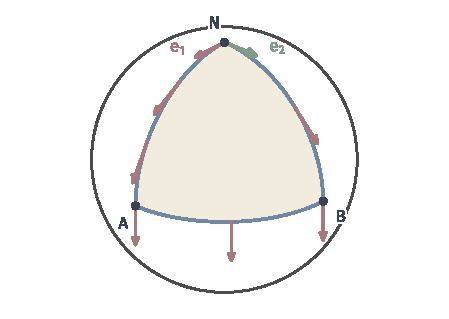
\includegraphics[width=76mm]{figures/04-spaces-measures-and-geometry/04-manifolds/matplotlib/riem-octant-transport/figure.pdf}
  \caption{球面八分之一三角形$N\to A\to B\to N$（黄色）上的平行移动。红箭头是例~\ref{ex:riem-sphere-transport}给出的向量$V(t)$，它沿每段大圆保持与路线的固定夹角；回到$N$时变为绿箭头$\bm e_2$，与初始的$\bm e_1$成直角。}
  \label{fig:riem-octant-transport}
\end{BookInlineFigure}

转角恰好等于这块球面三角形的面积$4\pi/8=\pi/2$。这个巧合在下面的例子中再次出现，第~\ref{sec:riem-curvature}节将用曲率解释。

\begin{example}[沿纬线的平行移动]
\label{ex:riem-latitude-transport}
沿过$p=(0,\tfrac35,\tfrac45)$的纬线搬运一个切向量。记$\theta_0$为$p$的极角，
\[
\sin\theta_0=\tfrac35,\qquad\cos\theta_0=\tfrac45 .
\]
路线取$(\theta,\phi)=(\theta_0,\tfrac\pi2+t)$，$t\in[0,2\pi]$。此时$\dot\theta=0$、$\dot\phi=1$，方程~\eqref{eq:riem-parallel-equation}化为
\[
\dot V_\theta=\sin\theta_0\cos\theta_0\,V_\phi,\qquad\dot V_\phi=-\cot\theta_0\,V_\theta .
\]

$\partial_\phi$的长度是$\sin\theta_0$，改用单位向量的分量会更清楚。令
\[
\bm e_\theta=\partial_\theta,\qquad\bm e_\phi=\frac{\partial_\phi}{\sin\theta_0},\qquad V=a\,\bm e_\theta+b\,\bm e_\phi ,
\]
则$V_\theta=a$，$V_\phi=b/\sin\theta_0$，代入得到
\[
\dot a=\cos\theta_0\,b,\qquad\dot b=-\cos\theta_0\,a .
\]

这是匀速旋转的方程。取初值$a(0)=1$、$b(0)=0$，也就是$p$处指向南方的单位向量，解为
\[
a(t)=\cos(\tfrac45t),\qquad b(t)=-\sin(\tfrac45t).
\]

绕一圈回到$p$时$t=2\pi$，$\tfrac45t=\tfrac{8\pi}5$，于是
\[
a(2\pi)=\cos\tfrac{2\pi}5\approx0.309,\qquad b(2\pi)=\sin\tfrac{2\pi}5\approx0.951 .
\]
向量从$\bm e_\theta$朝$\bm e_\phi$方向转过了$\tfrac{2\pi}5$。北极冠的面积是$2\pi(1-\cos\theta_0)=\tfrac{2\pi}5$，转角再次等于所围面积。
\end{example}

纬线的例子还可以用一张平面图来理解。沿纬线作球面的切锥，切点处锥面与球面有相同的切平面。对沿纬线的向量场，平行的条件只是“$\dot V$垂直于切平面”，所以在球面上平行与在切锥上平行是同一个条件。切锥可以摊平成平面扇形，半径$\tan\theta_0=\tfrac34$，圆心角$2\pi\cos\theta_0=\tfrac{8\pi}5$。在摊平的扇形上，平行向量就是常向量。

图~\ref{fig:riem-latitude-transport}(b)就是这个扇形：红箭头在平面上始终平行，$p$在扇形的两条边上各出现一次。扇形的缺口恰好是$\tfrac{2\pi}5$，这正是绕一圈的转角。

\begin{BookInlineFigure}
  \centering
  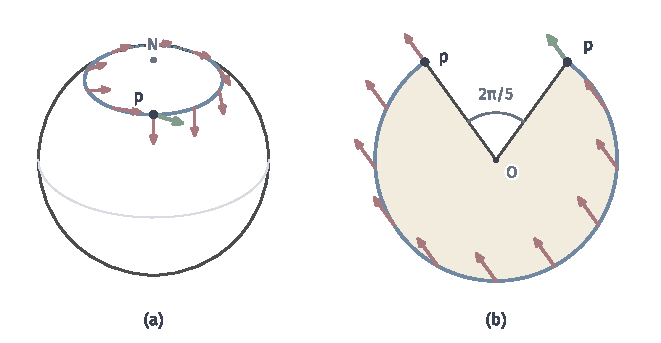
\includegraphics[width=112mm]{figures/04-spaces-measures-and-geometry/04-manifolds/matplotlib/riem-latitude-transport/figure.pdf}
  \caption{沿纬线的平行移动。(a)过$p=(0,\tfrac35,\tfrac45)$的纬线（蓝色）上，红箭头是从向南的单位向量出发平行移动的结果，绕一圈回到$p$时变为绿箭头，转过$\tfrac{2\pi}5$。(b)切锥摊平成的扇形，圆心角$\tfrac{8\pi}5$，缺口$\tfrac{2\pi}5$，纬线是外圆弧，$O$是锥顶。沿纬线的平行向量在扇形上是常向量，两条边是锥面上同一条母线。}
  \label{fig:riem-latitude-transport}
\end{BookInlineFigure}

\paragraph{与映射的微分比较}
第~\ref{chap:manifold-maps}章中，光滑映射$F:M\to N$在每点诱导线性映射$\mathrm dF_p:T_pM\to T_{F(p)}N$。平行移动$P_\gamma$也是切空间之间的线性映射，但二者的输入完全不同，表~\ref{tab:riem-transport-vs-differential}列出了对照。

\begin{BookInlineTable}
  \centering
  \begin{tabular}{lll}
    \toprule
    & 微分$\mathrm dF_p$ & 平行移动$P_\gamma$\\
    \midrule
    需要的输入 & 点映射$F$ & 曲线$\gamma$与联络\\
    是否需要度量 & 不需要 & 取Levi-Civita联络时需要\\
    依赖的范围 & $F$在$p$附近的取值 & 整条曲线\\
    \bottomrule
  \end{tabular}
  \caption{切空间之间的两种线性映射。}
  \label{tab:riem-transport-vs-differential}
\end{BookInlineTable}

在欧氏平面上取绕原点旋转角$\alpha$的映射$F$，则$\mathrm dF_p\bm v=\bm R_\alpha\bm v$，向量随之转过$\alpha$。而沿任何从$p$到$F(p)$的曲线作平行移动，得到的都是$\bm v$本身。两者都把$T_pM$映到$T_{F(p)}M$，结果却相差一个旋转。后面讨论等距映射与Lie群作用时，需要分清向量是“被映射带过去”还是“沿路径搬过去”的。

\section{测地线的初值问题}
\label{sec:riem-geodesic-ivp}

在平面上，“一直向前走”就是沿直线匀速运动，加速度为零。在球面上照搬这个说法会出问题：从$p=(1,0,0)$沿切方向$v=(0,1,0)$走直线$p+tv$，长度$\sqrt{1+t^2}$大于$1$，立刻离开球面。沿赤道$\gamma(t)=(\cos t,\sin t,0)$匀速前进则始终留在球面上，它的环境加速度$\ddot\gamma=-\gamma$不为零，却完全指向球面法向，只是“贴住球面”所必需的。沿球面没有转弯，意味着加速度的切向部分为零，也就是速度的协变导数为零。

\begin{definition}[测地线]
\label{def:riem-geodesic}
黎曼流形$(M,g)$上的光滑曲线$\gamma:I\to M$（$I$为区间）若满足
\[
\frac{D\dot\gamma}{\mathrm dt}=0,
\]
其中协变导数取Levi-Civita联络，就称$\gamma$为\term{测地线}（geodesic）。换言之，测地线的速度沿它自身平行移动。
\end{definition}

由定理~\ref{thm:riem-transport-isometry}，速度的长度沿测地线不变，所以测地线总是匀速的。这也意味着“测地线”是带参数化的概念：赤道换成非匀速参数化$t\mapsto(\cos t^3,\sin t^3,0)$，像集不变，速度大小却在变化，因此不再满足定义；只有仿射换元$t=as+b$保持测地线方程。本节先研究由初始位置和初始速度确定测地线的微分方程，再用指数映射把从一点出发的所有测地线汇总起来。

\subsection{测地线方程}
\label{sec:riem-geodesic-equation}

在坐标图中写$\gamma(t)$的坐标为$x(t)$，则$\dot\gamma=\sum_j\dot x^j\partial_j$。在式\eqref{eq:riem-covariant-derivative-along-curve}中取$V=\dot\gamma$，即$V^j=\dot x^j$，测地线条件化为
\begin{equation}
\ddot x^k(t)+\sum_{i,j=1}^n\Gamma^k_{i,j}\bigl(x(t)\bigr)\,\dot x^i(t)\,\dot x^j(t)=0,\qquad k=1,\ldots,n .
\label{eq:riem-geodesic-equation}
\end{equation}
与平行移动方程\eqref{eq:riem-parallel-equation}不同，这里系数依赖未知的$x(t)$，方程关于速度是二次的，因此是非线性方程。

\begin{example}[极坐标中的直线与球面上的大圆]
\label{ex:riem-geodesic-examples}
欧氏平面的极坐标中，由例~\ref{ex:riem-christoffel-examples}，测地线方程为
\[
\ddot r-r\dot\theta^2=0,\qquad\ddot\theta+\frac2r\dot r\dot\theta=0 .
\]
直线$x=1$匀速参数化为$y=t$，对应$r=\sqrt{1+t^2}$、$\theta=\arctan t$。计算得$\dot r=t(1+t^2)^{-1/2}$、$\ddot r=(1+t^2)^{-3/2}$、$\dot\theta=(1+t^2)^{-1}$、$\ddot\theta=-2t(1+t^2)^{-2}$，代入两式均为零。直线在直角坐标中的方程$\ddot x=\ddot y=0$，在极坐标中出现了Christoffel项。

单位球面上，方程为
\[
\ddot\theta-\sin\theta\cos\theta\,\dot\phi^2=0,\qquad\ddot\phi+2\cot\theta\,\dot\theta\dot\phi=0 .
\]
赤道$\theta=\pi/2$、$\phi=t$满足两式，是测地线。纬线$\theta=\theta_0\neq\pi/2$、$\phi=t$使第一式左端等于$-\sin\theta_0\cos\theta_0\neq0$，所以不是测地线：沿北半球的纬线匀速前进，需要一直向北侧转弯。
\end{example}

\paragraph{局部存在唯一与初值依赖}
把二阶方程改写成关于$(x,\dot x)$的一阶系统$\dot x=w$、$\dot w^k=-\sum_{i,j}\Gamma^k_{i,j}(x)w^iw^j$，右端是$(x,w)$的光滑函数。对这类方程，下面的结论成立，证明同样归入前面所引的卷六相应章节。

\begin{theorem}[光滑常微分方程的局部理论]
\label{thm:riem-smooth-ode}
设$W\subseteq\mathbb R^m$开，$F:W\to\mathbb R^m$光滑。则对每个$y_0\in W$：
\begin{enumerate}
\item 存在$\varepsilon>0$及唯一的解$y:(-\varepsilon,\varepsilon)\to W$，满足$\dot y=F(y)$、$y(0)=y_0$；
\item 两个解在公共定义区间上若有一个时刻取值相同，则在整个公共区间上相同，因而所有解可以拼成唯一的最大解，其定义区间是包含$0$的开区间；
\item 最大解$y(t;y_0)$关于$(t,y_0)$光滑，所有使其有定义的$(t,y_0)$构成开集；
\item 若最大解的定义区间右端点$t^+$有限，则当$t\to t^+$时$y(t)$终将离开$W$的每个紧子集。
\end{enumerate}
\end{theorem}

应用到测地线方程，得到：对每个$p\in M$和$v\in T_pM$，存在唯一的最大测地线$\gamma_v:I_v\to M$，满足$\gamma_v(0)=p$、$\dot\gamma_v(0)=v$，其中$I_v$是包含$0$的开区间。跨图时的拼接与平行移动相同，由唯一性保证一致。光滑依赖说明，初始速度稍有变化，测地线在有限时间内的位置也只稍有变化。

\paragraph{初始速度与时间的换算}
初始速度放大$c$倍，等价于把时间加快$c$倍：对$c\neq0$，$t\mapsto\gamma_v(ct)$满足测地线方程，初值为$p$与$cv$，所以
\begin{equation}
\gamma_{cv}(t)=\gamma_v(ct),\qquad t\in I_{cv}=\tfrac1cI_v .
\label{eq:riem-geodesic-rescaling}
\end{equation}
验证只需注意方程\eqref{eq:riem-geodesic-equation}的每一项关于时间导数是二次齐次的：$\ddot x$与$\dot x^i\dot x^j$都乘上$c^2$。

\paragraph{局部解未必能延拓到所有时间}
定理~\ref{thm:riem-smooth-ode}只保证解在某个时间区间内存在。在开单位球$M=\{x\in\mathbb R^n:\lVert x\rVert_2<1\}$上取欧氏度量，测地线是匀速直线。从原点以速度$2\bm e_1$出发，$\gamma(t)=2t\bm e_1$只在$t\in(-1/2,1/2)$内留在$M$中，最大定义区间是有限的；这正是结论(4)所说的“离开每个紧子集”。完整的单位球面上则不同，大圆对所有实数时间都有定义。测地线能否延拓到所有时间，取决于流形的整体性质，第~\ref{sec:riem-shortest-paths}节的Hopf--Rinow定理回答这个问题。

\subsection{黎曼指数映射}
\label{sec:riem-exponential-map}

从一点$p$出发，每个初始速度$v$给出一条测地线。把“沿$v$方向走单位时间到达哪里”记录下来，就得到从切空间$T_pM$到流形的一个映射。它把$p$附近的点用一个切向量来标记，类似于在地图上用“方向和距离”标记位置。

\begin{definition}[黎曼指数映射]
\label{def:riem-exponential-map}
对$p\in M$，令$\mathcal E_p=\{v\in T_pM:1\in I_v\}$为测地线$\gamma_v$至少存在到时刻$1$的初速度全体。定义
\[
\exp_p:\mathcal E_p\to M,\qquad\exp_p(v)=\gamma_v(1),
\]
称为$p$处的\term{黎曼指数映射}（Riemannian exponential map）。
\end{definition}

由式\eqref{eq:riem-geodesic-rescaling}，若$v\in\mathcal E_p$且$0\leq t\leq1$，则$tv\in\mathcal E_p$，并且
\[
\exp_p(tv)=\gamma_{tv}(1)=\gamma_v(t).
\]
所以沿射线$t\mapsto tv$的像正是测地线$\gamma_v$，定义域$\mathcal E_p$关于原点呈星形。由定理~\ref{thm:riem-smooth-ode}的结论(3)，$\mathcal E_p$是包含$0$的开集，$\exp_p$在其上光滑。

\begin{theorem}[指数映射的局部可逆性]
\label{thm:riem-exp-local-diffeo}
对每个$p\in M$，$d(\exp_p)_0:T_0(T_pM)\cong T_pM\to T_pM$是恒等映射。因此存在$0$在$T_pM$中的开邻域$V$和$p$在$M$中的开邻域$U$，使$\exp_p:V\to U$是微分同胚。
\end{theorem}

\begin{proof}
线性空间$T_pM$在$0$处的切空间可以认同为$T_pM$本身。对$v\in T_pM$，曲线$t\mapsto tv$在$t=0$的速度是$v$，它在$\exp_p$下的像是$\gamma_v(t)$，速度为$\dot\gamma_v(0)=v$。由链式法则，$d(\exp_p)_0(v)=v$。微分在一点可逆，由反函数定理即得局部微分同胚；反函数定理的欧氏形式可参考\BookChapterRef{chap:implicit-inverse-functions}{卷二“隐函数与反函数”章}，它在流形上的形式见第~\ref{chap:manifold-relations}章。
\end{proof}

若$V$还可以取为关于原点星形的，例如以$0$为心的球$\{v:\lVert v\rVert_g<\varepsilon\}$，则称像集$U=\exp_p(V)$为$p$的\term{正常邻域}（normal neighborhood）。在正常邻域中，每个点$q$都唯一地写成$q=\exp_p(v)$，$v\in V$，从$p$到$q$有一条“径向”测地线$t\mapsto\exp_p(tv)$。取$T_pM$的一组标准正交基把$v$写成坐标，就得到$U$上的一组坐标，称为$p$处的法坐标。

\begin{example}[单位球面的指数映射]
\label{ex:riem-sphere-exp}
单位球面$\mathbb S^{n}\subseteq\mathbb R^{n+1}$上，取$p$与$v\perp p$，$r=\lVert v\rVert_2>0$。曲线$\gamma(t)=\cos(tr)\,p+\sin(tr)\,v/r$满足$\lVert\gamma(t)\rVert_2=1$，$\gamma(0)=p$，$\dot\gamma(0)=v$，且$\ddot\gamma=-r^2\gamma$为纯法向，所以它是测地线。于是$\mathcal E_p=T_p\mathbb S^n$，并且
\[
\exp_p(v)=\cos\lVert v\rVert_2\,p+\frac{\sin\lVert v\rVert_2}{\lVert v\rVert_2}\,v,\qquad\exp_p(0)=p .
\]
所有长度为$\pi$的初速度都到达对跖点$-p$，所以$\exp_p$不是单射；在开球$\lVert v\rVert_2<\pi$上它是到$\mathbb S^n\setminus\{-p\}$的微分同胚。可见即使指数映射处处有定义，可逆性也只是局部的。
\end{example}

\paragraph{与矩阵指数的区别}
第~\ref{chap:lie-groups}章会在矩阵Lie群上用矩阵指数$e^{\bm A}=\sum_k\bm A^k/k!$把单位元处的切向量变成群元素。两者都叫“指数”，都从切空间出发、在零点处微分为恒等，但来源不同：黎曼指数映射由度量经Levi-Civita联络确定，换一个度量就会改变；矩阵指数只由群的乘法确定，不需要度量。在带特殊度量的某些群上二者可以一致，这需要单独验证，不能仅凭名称相同就互相替代。

\section{给定端点的最短路径}
\label{sec:riem-shortest-paths}

上一节固定的是起点和初始速度，本节固定的是两个端点。问题变成：在所有连接$p$与$q$的分段光滑曲线中，长度能否达到内在距离$d_g(p,q)$，达到时曲线是什么样子。我们分三步回答。先比较长度与能量，说明长度最短且匀速的曲线满足测地线方程；再证明足够短的测地线确实最短；最后陈述保证最短曲线存在的整体条件。每一步的结论都比前一步的要求多，不能互相替代。

\subsection{长度与能量的变分}
\label{sec:riem-length-energy-variation}

长度的被积函数$\lVert\dot\gamma\rVert_g$含有平方根，直接求导不便，而且长度对任何单调换参数都不变，同一条路线有无穷多种参数化都是“最优”的。常用的办法是改用能量。对$\gamma:[a,b]\to M$，定义\term{曲线能量}（energy of a curve）
\begin{equation}
E(\gamma)=\frac12\int_a^b\lVert\dot\gamma(t)\rVert_g^2\,\mathrm dt .
\label{eq:riem-energy}
\end{equation}

\paragraph{长度与能量的比较}
由Cauchy--Schwarz不等式，把$\lVert\dot\gamma\rVert_g$看成与常函数$1$作内积：
\[
L_g(\gamma)^2=\Bigl(\int_a^b1\cdot\lVert\dot\gamma\rVert_g\,\mathrm dt\Bigr)^2\leq(b-a)\int_a^b\lVert\dot\gamma\rVert_g^2\,\mathrm dt .
\]
右端等于$2(b-a)E(\gamma)$，所以
\begin{equation}
L_g(\gamma)^2\leq2(b-a)E(\gamma),
\label{eq:riem-length-energy}
\end{equation}
等号成立当且仅当$\lVert\dot\gamma\rVert_g$在$[a,b]$上几乎处处为常数，即曲线匀速。

因此在固定时间区间上，走同一条路线时忽快忽慢只会增加能量。例如在实数轴上走$[0,1]$这段路线，$x(t)=t^2$，$t\in[0,1]$，长度$L=1$，能量却是
\[
E=\frac12\int_0^1(2t)^2\,\mathrm dt=\frac23 .
\]
匀速的$x(t)=t$给出$E=\tfrac12=L^2/2$，式~\eqref{eq:riem-length-energy}取等号。能量最小的曲线必然匀速。速度处处非零的曲线可以重新参数化为匀速，所以在匀速曲线之间比较能量，等同于比较长度。

\paragraph{能量的驻定条件}
现在考察端点固定的扰动。设$\gamma$落在一张坐标图内，坐标为$x(t)$；取光滑的$h:[a,b]\to\mathbb R^n$，$h(a)=h(b)=0$，对足够小的$\varepsilon$令$x_\varepsilon=x+\varepsilon h$。若对所有这样的$h$都有
\[
\frac{\mathrm d}{\mathrm d\varepsilon}E(\gamma_\varepsilon)\Big|_{\varepsilon=0}=0,
\]
就称$\gamma$是能量的驻定曲线。

能量的被积函数是
\[
\mathscr L(x,\dot x)=\frac12\sum_{i,j}g_{i,j}(x)\,\dot x_i\dot x_j .
\]
对这类积分，所用的结论是Euler--Lagrange关系：若$\mathscr L$光滑，$x$为$C^2$曲线，则$x$在端点固定的扰动下驻定当且仅当
\begin{equation}
\frac{\partial\mathscr L}{\partial x_k}-\frac{\mathrm d}{\mathrm dt}\frac{\partial\mathscr L}{\partial\dot x_k}=0,\qquad k=1,\ldots,n .
\label{eq:riem-euler-lagrange}
\end{equation}
它的推导是对$\varepsilon$求导后分部积分，边界项因$h(a)=h(b)=0$消失，再由$h$的任意性得到被积系数为零；一般泛函的变分理论可参考\BookChapterRef{chap:functional-optimization-variation}{卷五“泛函优化与变分”章}。

把能量代入。对$x_k$和$\dot x_k$分别求偏导，
\[
\frac{\partial\mathscr L}{\partial x_k}=\frac12\sum_{i,j}\partial_kg_{i,j}\,\dot x_i\dot x_j,\qquad
\frac{\partial\mathscr L}{\partial\dot x_k}=\sum_jg_{k,j}\dot x_j .
\]

后一式对时间求导，用链式法则：
\[
\frac{\mathrm d}{\mathrm dt}\sum_jg_{k,j}\dot x_j=\sum_jg_{k,j}\ddot x_j+\sum_{i,j}\partial_ig_{k,j}\,\dot x_i\dot x_j .
\]
第二项对$i,j$对称化，写成$\frac12\sum_{i,j}(\partial_ig_{k,j}+\partial_jg_{k,i})\dot x_i\dot x_j$。

代回式~\eqref{eq:riem-euler-lagrange}并取负号，得到
\[
\sum_jg_{k,j}\ddot x_j+\frac12\sum_{i,j}\bigl(\partial_ig_{k,j}+\partial_jg_{k,i}-\partial_kg_{i,j}\bigr)\dot x_i\dot x_j=0 .
\]
括号恰是式~\eqref{eq:riem-christoffel}中的组合。两边乘$\bm G^{-1}$，得到测地线方程~\eqref{eq:riem-geodesic-equation}。曲线跨越多张图时，用支撑在单张图内的扰动逐段推导，结论相同。

单位球面可以这样快速验算。被积函数是
\[
\mathscr L=\tfrac12\bigl(\dot\theta^2+\sin^2\theta\,\dot\phi^2\bigr).
\]

对$\theta$和对$\phi$的方程分别是
\[
\ddot\theta-\sin\theta\cos\theta\,\dot\phi^2=0,\qquad
\frac{\mathrm d}{\mathrm dt}\bigl(\sin^2\theta\,\dot\phi\bigr)=0 .
\]
第二式展开后就是例~\ref{ex:riem-geodesic-examples}中的第二个方程。

这样得到两条结论。光滑曲线是能量的驻定曲线，当且仅当它是测地线。若匀速曲线在所有连接相同端点的曲线中长度最短，则它也是能量最小的，因而是测地线。长度本身的驻定曲线则只确定路线、不确定参数化：长度的Euler--Lagrange方程对任意换参数都成立，换成匀速参数后才是测地线方程。

\paragraph{驻定不等于最短}
驻定条件只是一阶条件，类似卷一中导数为零的点不一定是最小值点。完整单位圆上，从$(1,0)$到$(0,-1)$，顺时针的短弧长$\pi/2$，逆时针的长弧长$3\pi/2$，二者匀速参数化后都是测地线，只有前者最短。单位球面上沿大圆从$p$出发走过对跖点再继续，同样是测地线，却比反方向的另一段大圆弧长。驻定曲线是否最短，还要额外比较。

\subsection{局部最短性}
\label{sec:riem-local-minimality}

上面的反例都发生在曲线较长时。下面证明：足够短的测地线一定最短。论证用到正常邻域中径向与“横向”方向的正交关系。平面上，同心圆与半径处处垂直；下面的Gauss引理说明，在指数映射的图像里同样如此。

\begin{lemma}[Gauss引理]
\label{lem:riem-gauss-lemma}
设$\exp_p$在$T_pM$中以$\bm 0$为心、半径$\varepsilon$的球$B_\varepsilon(\bm 0)$上是微分同胚。对$\bm v\in B_\varepsilon(\bm 0)$，$\bm v\neq\bm 0$，以及任意$\bm w\in T_pM$，有
\begin{equation}
g\bigl(\mathrm d(\exp_p)_{\bm v}(\bm v),\,\mathrm d(\exp_p)_{\bm v}(\bm w)\bigr)=g_p(\bm v,\bm w).
\label{eq:riem-gauss-lemma}
\end{equation}
特别地，径向测地线的速度与由长度等于$\lVert\bm v\rVert_g$的切向量在$\exp_p$下的像组成的球面在交点处正交。
\end{lemma}

\begin{proof}
构造一族从$p$出发的测地线：对$t\in[0,1]$和足够小的$s$，令
\[
f(t,s)=\exp_p\bigl(t(\bm v+s\bm w)\bigr).
\]
$f$是光滑的，固定$s$时它是初速度为$\bm v+s\bm w$的测地线。记$T=\partial_tf$，$S=\partial_sf$，这是沿这族曲线的两个向量场。

我们需要两个事实。第一，$T$沿$t$方向的协变导数为零，这是测地线方程：$D_tT=0$。第二，$D_tS=D_sT$，这是无挠条件的结果。在坐标中，$D_tS$的$k$分量是
\[
\frac{\partial^2x_k}{\partial t\,\partial s}+\sum_{i,j}\Gamma^k_{i,j}\frac{\partial x_i}{\partial t}\frac{\partial x_j}{\partial s},
\]
由$\Gamma^k_{i,j}$的对称性，它关于$t,s$对称。

对$g(T,S)$关于$t$求导，用度量相容和上面两个事实：
\[
\partial_t\,g(T,S)=g(D_tT,S)+g(T,D_tS)=g(T,D_sT).
\]

右端等于$\tfrac12\partial_s\,g(T,T)$。测地线匀速，所以$g(T,T)$等于初速度的长度平方$\lVert\bm v+s\bm w\rVert_g^2$，与$t$无关。取$s=0$，得到
\[
\partial_t\,g(T,S)\big|_{s=0}=\tfrac12\frac{\mathrm d}{\mathrm ds}\lVert\bm v+s\bm w\rVert_g^2\Big|_{s=0}=g_p(\bm v,\bm w).
\]

右端是常数。在$t=0$处，$f(0,s)=p$与$s$无关，所以$S(0,0)=\bm 0$，$g(T,S)$从$0$开始。沿$t$积分到$t=1$，得到
\[
g(T,S)\big|_{(1,0)}=g_p(\bm v,\bm w).
\]
而$T(1,0)=\mathrm d(\exp_p)_{\bm v}(\bm v)$，$S(1,0)=\mathrm d(\exp_p)_{\bm v}(\bm w)$，这就是式~\eqref{eq:riem-gauss-lemma}。

取$\bm w$与$\bm v$垂直，右端为零，所以径向方向与测地球面垂直。
\end{proof}

称$\exp_p(B_\varepsilon(\bm 0))$为$p$的半径$\varepsilon$的测地球。Gauss引理把图~\ref{fig:riem-exp-map}(c)的分解变成了等式：速度分解成径向和横向两部分，二者互相垂直，勾股定理可以用。

\begin{theorem}[径向测地线的最短性]
\label{thm:riem-radial-minimizing}
设$\exp_p$在$B_\varepsilon(\bm 0)\subseteq T_pM$上是微分同胚，$q=\exp_p(\bm v)$，$\lVert\bm v\rVert_g<\varepsilon$。则径向测地线$\sigma(t)=\exp_p(t\bm v)$，$t\in[0,1]$，长度为$\lVert\bm v\rVert_g$，并且任何从$p$到$q$的分段光滑曲线长度都不小于$\lVert\bm v\rVert_g$。因此
\begin{equation}
d_g(p,q)=\lVert\bm v\rVert_g .
\label{eq:riem-radial-distance}
\end{equation}
\end{theorem}

\begin{proof}
$\sigma$是初速度为$\bm v$的测地线，匀速，所以$L_g(\sigma)=\lVert\bm v\rVert_g$。设$\gamma:[a,b]\to M$是任一从$p$到$q$的分段光滑曲线。可以假设$\gamma$在$t>a$时不再经过$p$，否则从最后一次经过$p$的时刻开始考虑，长度只会变小。

先设$\gamma$始终留在测地球中。对$t>a$写
\[
\gamma(t)=\exp_p\bigl(\rho(t)\bm u(t)\bigr),\qquad\rho(t)>0,\quad\lVert\bm u(t)\rVert_g=1 .
\]

由链式法则，
\[
\dot\gamma=\mathrm d(\exp_p)\bigl(\dot\rho\,\bm u+\rho\,\dot{\bm u}\bigr),
\]
其中$\dot{\bm u}\perp\bm u$，因为$\lVert\bm u\rVert_g$恒为$1$。在式~\eqref{eq:riem-gauss-lemma}中取$\bm v=\rho\bm u$、$\bm w=\bm u$，得到$\mathrm d(\exp_p)(\bm u)$的长度为$1$。再取$\bm w=\rho\dot{\bm u}$，得到它与$\mathrm d(\exp_p)(\rho\dot{\bm u})$正交。

于是两部分互相垂直，由勾股定理，
\[
\lVert\dot\gamma\rVert_g^2=\dot\rho^2+\bigl\lVert\mathrm d(\exp_p)(\rho\dot{\bm u})\bigr\rVert_g^2\geq\dot\rho^2 .
\]

积分，并让积分下限趋于$a$（此时$\rho\to0$），得到
\[
L_g(\gamma)\geq\int_a^b\lvert\dot\rho\rvert\,\mathrm dt\geq\rho(b)-\lim_{t\to a^+}\rho(t)=\lVert\bm v\rVert_g .
\]

若$\gamma$离开测地球，它在离开前必须先到达每个半径$\delta<\varepsilon$的测地球面。对满足$\lVert\bm v\rVert_g<\delta<\varepsilon$的$\delta$，把上面的论证用于从$p$到第一次到达半径$\delta$球面的那一段，得到$L_g(\gamma)\geq\delta>\lVert\bm v\rVert_g$。两种情形合起来即得结论。
\end{proof}

证明中的不等式还给出等号条件：长度恰为$\lVert\bm v\rVert_g$的曲线必须$\rho$单调、横向分量为零，也就是沿径向走。所以测地球内$p$到$q$的最短曲线，除参数化外只有径向测地线这一条。

定理比较的是从中心$p$出发的所有曲线，包括离开测地球的曲线，所以结论是真正的距离等式。它对测地球中任意两点之间的连线并不直接给出结论：两点都不是中心时，需要更小的凸正常邻域，在那里任意两点由唯一一条留在邻域内的最短测地线连接。这一进一步的局部结论的证明较长，读者可查阅Lee的教材\scite{math-lee2018riemannian}。称长度等于两端点内在距离的测地线为\term{最短测地线}（minimizing geodesic）。

\paragraph{局部最短不意味着全局最短或唯一}
定理~\ref{thm:riem-radial-minimizing}给出：每条测地线的足够短的一段都是最短测地线。但整条测地线可以不是最短的。取半径为$1$的圆柱面$\{(x,y,z):x^2+y^2=1\}$，曲线$t\mapsto(\cos t,\sin t,ct)$匀速，环境加速度$(-\cos t,-\sin t,0)$沿法向，所以这些螺旋线是测地线。

考虑连接$p_0=(1,0,0)$与$p_1=(1,0,\pi)$的曲线。竖直线段长$\pi$。绕$k$圈的螺旋线$t\mapsto(\cos t,\sin t,\tfrac{t}{2k})$，$t\in[0,2\pi k]$，速率是$\sqrt{1+1/(4k^2)}$，长度为
\[
L_k=2\pi k\sqrt{1+\frac1{4k^2}}=\pi\sqrt{4k^2+1}.
\]
$k=1,2$时分别是$\pi\sqrt5\approx7.02$和$\pi\sqrt{17}\approx12.95$，反向绕圈的情形相同。连接同一对端点的测地线有无穷多条，局部都是最短的，只有竖直线段全局最短。

图~\ref{fig:riem-cylinder-geodesics}把这些曲线放到圆柱展开的平面上：$p_1$有无穷多个“复本”，每条测地线就是通向其中一个复本的直线段。球面的对跖点则说明，最短测地线本身也可以不唯一：所有从$p$到$-p$的半个大圆都是最短的。

\begin{BookInlineFigure}
  \centering
  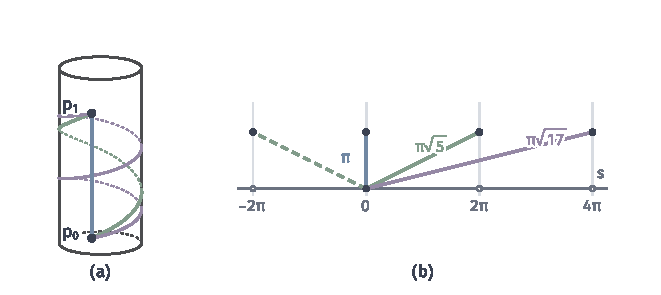
\includegraphics[width=112mm]{figures/04-spaces-measures-and-geometry/04-manifolds/matplotlib/riem-cylinder-geodesics/figure.pdf}
  \caption{圆柱面上连接同一对点的多条测地线。(a)单位圆柱上的$p_0=(1,0,0)$、$p_1=(1,0,\pi)$，蓝色竖直线段长$\pi$，绿色、紫色分别绕$1$圈、$2$圈。(b)沿圆周方向展开，竖线是$s=2\pi k$处$p_0$与$p_1$的复本，每条测地线是从原点到一个复本的线段，长度分别为$\pi$、$\pi\sqrt5$、$\pi\sqrt{17}$；虚线是反向绕圈的情形。}
  \label{fig:riem-cylinder-geodesics}
\end{BookInlineFigure}

\subsection{最短路径的存在}
\label{sec:riem-shortest-existence}

局部最短性只回答“短距离内测地线就是最短路”，不回答相距较远的两点之间是否有最短路。图~\ref{fig:riem-punctured-plane}的穿孔平面表明，答案可以是否定的：缺口使逼近下确界的曲线序列没有极限。排除这类缺口的条件是度量完备性。

\begin{theorem}[Hopf--Rinow定理]
\label{thm:riem-hopf-rinow}
设$(M,g)$是有限维、连通、无边界的黎曼流形。下列条件等价：
\begin{enumerate}
\item 度量空间$(M,d_g)$完备；
\item $M$是\term{测地完备}（geodesically complete）的，即每条测地线都能延拓到全体实数时间；
\item 存在某一点$p$，使$\exp_p$在整个$T_pM$上有定义；
\item $M$中有界闭集都是紧集。
\end{enumerate}
满足这些条件时，任意两点$p,q\in M$之间存在长度为$d_g(p,q)$的最短测地线。
\end{theorem}

这一定理称为\term{Hopf--Rinow定理}（Hopf--Rinow theorem）。证明需要依次比较几种完备性，篇幅较长，读者可查阅前引教材。它的机制可以这样理解：条件(3)使从$p$出发的每个方向都能一直走下去。对远处的点$q$，在$p$附近的测地球面上取与$q$距离最小的点，沿指向它的方向走测地线，可以证明这条测地线一直“对准”$q$，走过距离$d_g(p,q)$时恰好到达$q$。完备性保证这一过程不会中途掉进缺口。

\paragraph{条件的作用}
紧的无边界黎曼流形总是完备的：紧度量空间中的Cauchy列有收敛子列，从而本身收敛（第~\ref{chap:metric-spaces}章）。所以球面、环面等闭曲面上任意两点之间都有最短测地线。穿孔平面与开单位球不完备：前者中趋于原点的点列是Cauchy列却不收敛，后者中直线测地线在有限时间到达缺失的边界。

定理的最后结论只是充分条件。开单位球不完备，但它是凸集，任意两点之间的线段留在球内，是最短测地线；穿孔平面则连这一点也做不到。所以“任意两点都有最短路”不能反推完备性，而缺少完备性时，最短路是否存在要具体判断。

\paragraph{存在与唯一}
Hopf--Rinow定理保证存在，不保证唯一。球面对跖点之间有无穷多条最短测地线，圆柱面上位于同一水平圆的对径点之间有两条。存在性也不能由测地线方程的局部存在唯一性推出：后者固定的是初始速度，回答的是“从这个方向出发会走到哪里”；端点问题要找的是“哪个初始速度能恰好到达$q$且最短”，这需要比较全部路线，依赖流形的整体结构。

\section{曲率}
\label{sec:riem-curvature}

例~\ref{ex:riem-sphere-transport}中，球面上绕一圈平行移动回到起点，向量转过了$\pi/2$；平面上无论怎样绕，向量都不变。这个差别不是坐标造成的，而是两种几何本身不同。本节要找一个逐点定义、与坐标无关的量来检测它。思路是把绕圈缩小到无穷小：沿两个方向先后求协变导数，比较两种次序的结果。得到的曲率张量描述内在几何；最后再把它与曲面在环境空间中“看上去弯曲”的程度区分开。

\subsection{曲率张量与截面曲率}
\label{sec:riem-curvature-tensor}

在欧氏空间中，二阶偏导数可以交换次序。对向量场的协变导数，交换次序的差$\nabla_X\nabla_YZ-\nabla_Y\nabla_XZ$一般不为零，但其中有一部分来自方向场本身：即使在平面上，若$X,Y$不可交换，先沿$X$再沿$Y$与先沿$Y$再沿$X$也不会回到同一点。这部分差别由Lie括号$[X,Y]$描述，应当扣除。

\begin{definition}[黎曼曲率张量]
\label{def:riem-curvature-tensor}
设$\nabla$是$(M,g)$的Levi-Civita联络。对$X,Y,Z\in\mathfrak X(M)$定义
\begin{equation}
R(X,Y)Z=\nabla_X\nabla_YZ-\nabla_Y\nabla_XZ-\nabla_{[X,Y]}Z .
\label{eq:riem-curvature}
\end{equation}
$R$称为$(M,g)$的\term{黎曼曲率张量}（Riemann curvature tensor）。
\end{definition}

文献中曲率的符号约定不统一，有的教材把上式整体取负号。本书采用上式，在这一约定下单位球面的截面曲率为正，后面会核对。

\paragraph{曲率是逐点定义的}
式\eqref{eq:riem-curvature}的三项都含有导数，似乎需要知道$X,Y,Z$在一点附近的取值。实际上$R$对三个变量都按函数线性，所以$(R(X,Y)Z)(p)$只依赖$X_p,Y_p,Z_p$。以$Z$为例，把$fZ$代入，由乘积法则
\[
\nabla_X\nabla_Y(fZ)=(XYf)Z+(Yf)\nabla_XZ+(Xf)\nabla_YZ+f\nabla_X\nabla_YZ .
\]
交换$X,Y$后相减，中间两项抵消，第一项变为$([X,Y]f)Z$；而$\nabla_{[X,Y]}(fZ)=([X,Y]f)Z+f\nabla_{[X,Y]}Z$，恰好消去这一项，剩下$fR(X,Y)Z$。对$X$的函数线性可以类似验证，第三项$\nabla_{[X,Y]}Z$在其中同样负责抵消导数项；对$Y$的情形由$R(X,Y)=-R(Y,X)$得到。因此对点$p$处的切向量$u,v,w$可以写$R(u,v)w\in T_pM$。

\paragraph{坐标表示}
取坐标基场代入，Lie括号项消失，由$\nabla_{\partial_i}\nabla_{\partial_j}\partial_k=\nabla_{\partial_i}\bigl(\sum_m\Gamma^m_{j,k}\partial_m\bigr)$展开，得到$R(\partial_i,\partial_j)\partial_k=\sum_\ell R^\ell_{i,j,k}\partial_\ell$，其中
\begin{equation}
R^\ell_{i,j,k}=\partial_i\Gamma^\ell_{j,k}-\partial_j\Gamma^\ell_{i,k}+\sum_m\bigl(\Gamma^m_{j,k}\Gamma^\ell_{i,m}-\Gamma^m_{i,k}\Gamma^\ell_{j,m}\bigr).
\label{eq:riem-curvature-coordinates}
\end{equation}
曲率由度量的二阶导数决定。若在某组坐标中$\bm G$为常矩阵，则所有Christoffel符号为零，$R=0$。反过来，系数不为零并不说明曲率非零：极坐标中Christoffel符号不为零，平面的曲率仍为零，因为$R$是张量，在直角坐标中为零就在任何坐标中为零。

\paragraph{截面曲率}
$R$有三个输入，信息较多。最常用的标量是在一个二维切平面上读出的曲率。

\begin{definition}[截面曲率]
\label{def:riem-sectional-curvature}
设$u,v\in T_pM$线性无关，它们张成的平面$\Pi$的\term{截面曲率}（sectional curvature）为
\begin{equation}
K(\Pi)=K(u,v)=\frac{g\bigl(R(u,v)v,u\bigr)}{g(u,u)g(v,v)-g(u,v)^2}.
\label{eq:riem-sectional-curvature}
\end{equation}
\end{definition}

分母是$u,v$张成的平行四边形面积的平方，由Cauchy--Schwarz不等式，它在$u,v$线性无关时为正。可以证明分子在把$(u,v)$换成同一平面的另一组基时，与分母乘上相同的因子，所以$K$只依赖平面$\Pi$；这一点用到$g(R(u,v)w,z)$关于$(u,v)$和关于$(w,z)$都反对称的性质，这里不展开。二维流形每点只有一个切平面，截面曲率就是一个函数，称为\term{Gauss曲率}（Gaussian curvature）。一维流形没有二维切平面，式\eqref{eq:riem-curvature}中的$R$恒为零。

\begin{example}[单位球面的曲率]
\label{ex:riem-sphere-curvature}
用例~\ref{ex:riem-christoffel-examples}的系数$\Gamma^\theta_{\phi,\phi}=-\sin\theta\cos\theta$、$\Gamma^\phi_{\theta,\phi}=\Gamma^\phi_{\phi,\theta}=\cot\theta$计算$R(\partial_\theta,\partial_\phi)\partial_\phi$。由式\eqref{eq:riem-curvature-coordinates}，其$\theta$分量为
\begin{equation*}
\begin{aligned}
R^\theta_{\theta,\phi,\phi}&=\partial_\theta\Gamma^\theta_{\phi,\phi}-\partial_\phi\Gamma^\theta_{\theta,\phi}+\sum_m\bigl(\Gamma^m_{\phi,\phi}\Gamma^\theta_{\theta,m}-\Gamma^m_{\theta,\phi}\Gamma^\theta_{\phi,m}\bigr)\\
&=(\sin^2\theta-\cos^2\theta)-0+0-\cot\theta\cdot(-\sin\theta\cos\theta)=\sin^2\theta,
\end{aligned}
\end{equation*}
其中只有$m=\phi$的一项$\Gamma^\phi_{\theta,\phi}\Gamma^\theta_{\phi,\phi}$非零；同样可算出$\phi$分量为零。于是$R(\partial_\theta,\partial_\phi)\partial_\phi=\sin^2\theta\,\partial_\theta$，分子$g(R(\partial_\theta,\partial_\phi)\partial_\phi,\partial_\theta)=\sin^2\theta$，分母$1\cdot\sin^2\theta-0=\sin^2\theta$，所以$K=1$。半径为$a$的球面按同样计算得$K=1/a^2$：球越大，曲率越小，越接近平面。
\end{example}

\paragraph{小回路上的平行移动}
曲率与绕圈搬运的联系可以这样表述。在$p$处取线性无关的$u,v$，在法坐标中沿边长为$s$的小“平行四边形”回路（依次沿$su$、$sv$、$-su$、$-sv$方向）平行移动，记所得的线性映射为$P_s:T_pM\to T_pM$。则当$s\to0$时
\[
P_s(w)=w-s^2R(u,v)w+o(s^2),
\]
首项的符号随绕行方向和曲率符号约定而变。这里只说明机制，不给出证明：每条边上的平行移动可以展开到二阶，四段复合时一阶项相互抵消，二阶项中剩下的正是两种求导次序之差。在单位球面北极取$u=\bm e_1$、$v=\bm e_2$，由球面上$R(u,v)w=g(v,w)u-g(u,w)v$（可由例~\ref{ex:riem-sphere-curvature}的结果连同对称性推出）得$R(u,v)$把$v$映到$u$、把$u$映到$-v$，是切平面内转过直角的线性映射。所以小回路的效应是一个与所围面积$s^2$成比例的小转动。

\paragraph{局部曲率与整体回路}
曲率是局部量，有限回路的总效应还受整体形状影响，不能简单地把一点的曲率乘上面积。一个清楚的例子是锥面。从平面上剪去圆心角为$\alpha$（$0<\alpha<2\pi$）的扇形，把两条剪边粘合，再去掉顶点，得到的曲面每一小块都可以摊平成平面的一块，所以曲率处处为零。然而沿绕顶点一周的回路平行移动，在摊开的扇形中向量保持不变，经过粘合边时却要按扇形张角旋转一次，回到出发点时向量转过角$\alpha$。没有曲率的区域上，绕不可收缩的回路仍可以有非平凡的平行移动；这是拓扑与局部几何共同造成的。

\subsection{内在曲率与嵌入弯曲}
\label{sec:riem-intrinsic-extrinsic}

日常说一个曲面“弯”，通常指它在三维空间中的形状。黎曼曲率衡量的则是曲面内部的长度规则能否摊平成平面。这两件事不同：一张纸可以卷成圆柱而不拉伸、不起皱，纸上的长度与角度保持不变；却无法不拉伸地包住一个球。

\paragraph{平面与圆柱}
取半径为$a$的圆柱面，局部参数化为
\begin{equation*}
\Phi(s,z)=(a\cos(s/a),a\sin(s/a),z),\qquad s\in(0,2\pi a).
\end{equation*}两列切向量为$(-\sin(s/a),\cos(s/a),0)$与$(0,0,1)$，都是单位向量且互相正交，所以诱导度量$\bm G=\bm I$。在这组坐标中Christoffel符号全为零，曲率张量为零，截面曲率$K=0$。就内在几何而言，圆柱面的这一块与平面的一个矩形没有区别。

圆柱在环境中的弯曲由法向量的变化体现。单位法向量为$n(s,z)=(\cos(s/a),\sin(s/a),0)$，沿$s$方向的导数是$\frac1a(-\sin(s/a),\cos(s/a),0)$，大小$1/a$；沿$z$方向不变。这两个数$1/a$与$0$称为曲面在该点的\term{主曲率}（principal curvature），它们描述法向量沿各方向转动的快慢，属于嵌入的性质。对半径为$a$的球面，法向量$n=x/a$沿任何单位切方向的导数大小都是$1/a$，两个主曲率都是$1/a$。

两种曲面的Gauss曲率与主曲率之间有一个关系：对$\mathbb R^3$中的曲面，Gauss曲率等于两个主曲率之积。圆柱给出$\frac1a\cdot0=0$，球面给出$\frac1{a^2}$，与前面的内在计算一致。这一关系称为Gauss绝妙定理，这里不给出证明；它的意义是，主曲率依赖嵌入，它们的乘积却只由诱导度量决定。

\paragraph{为什么要区分}
一维的例子更极端。半径为$a$的圆在平面中明显弯曲，法向偏离切线的程度由曲率$1/a$描述；可它的黎曼曲率恒为零，任何一段弧都与一段直线等距。所以，“法向量在变”“切平面在转”都不能作为内在曲率非零的证据，坐标中度量系数随位置变化也不能。反过来，内在平坦也不意味着嵌入不弯，圆柱就是例子。

这一区分在由采样点估计几何时很重要。第~\ref{chap:manifold-recovery}章用切平面拟合局部点云时，点到切平面的偏离量由法向量的变化，即嵌入弯曲控制，在圆或圆柱上也会出现；它反映的是嵌入的主曲率，而不是内在截面曲率。估计误差的分析须保持这一区分。

\section{等距映射}
\label{sec:riem-isometries}

前面各节都在一个黎曼流形内部讨论。圆柱的例子已经提出了比较两个黎曼流形的问题：圆柱的一块与平面的一块“内在几何相同”，这句话要怎样准确表述？第~\ref{chap:manifold-relations}章用微分同胚表达两个流形具有相同的光滑结构，但微分同胚可以任意拉伸长度。这里要求映射在每个切空间上保持内积。

\paragraph{保持内积的条件}
设$(M,g)$与$(N,h)$是黎曼流形，$F:M\to N$光滑。映射的微分$dF_p:T_pM\to T_{F(p)}N$把切向量从$p$带到$F(p)$。我们要求：任取$p\in M$及$u,v\in T_pM$，
\begin{equation}
g_p(u,v)=h_{F(p)}\bigl(dF_pu,\,dF_pv\bigr).
\label{eq:riem-isometry-condition}
\end{equation}
右端是用$N$的度量量出的、被带过去的两个向量的内积，左端是原来的内积。在坐标中，若$F$的Jacobian矩阵为$\bm J$，条件就是$\bm G_M=\bm J^{\top}\bm G_N\bm J$；这与式\eqref{eq:riem-induced-metric}形式相同，诱导度量正是让包含映射满足此条件的度量。

\begin{definition}[黎曼等距映射与等距浸入]
\label{def:riem-isometry}
满足式\eqref{eq:riem-isometry-condition}的微分同胚$F:M\to N$称为\term{黎曼等距映射}（Riemannian isometry），此时称$(M,g)$与$(N,h)$等距。满足式\eqref{eq:riem-isometry-condition}的光滑映射称为\term{等距浸入}（isometric immersion）。若每点都有邻域使$F$限制在其上是到像集（$N$的开集）的等距映射，就称$F$为\term{局部等距}（local isometry）。
\end{definition}

条件\eqref{eq:riem-isometry-condition}本身就迫使$dF_p$单射：若$dF_pu=0$，则$g_p(u,u)=0$，从而$u=0$。所以满足该条件的光滑映射自动是浸入，定义中的名称与第~\ref{chap:manifold-relations}章一致。当$\dim M=\dim N$时，等距浸入的微分是可逆线性映射，由反函数定理它就是局部等距。

\paragraph{等距映射保持什么}
等距浸入保持每条曲线的长度。设$\gamma$是$M$中的分段光滑曲线，$F\circ\gamma$的速度是$dF(\dot\gamma)$，由式\eqref{eq:riem-isometry-condition}，$\lVert dF(\dot\gamma)\rVert_h=\lVert\dot\gamma\rVert_g$，所以$L_h(F\circ\gamma)=L_g(\gamma)$。对等距映射还可以反过来用$F^{-1}$，于是两边的连接曲线一一对应且长度相同，取下确界即得
\[
d_h\bigl(F(p),F(q)\bigr)=d_g(p,q).
\]
等距映射还把Levi-Civita联络带到Levi-Civita联络，因而保持平行移动、测地线和曲率。理由是唯一性：用$F$把$N$上的联络拉回到$M$上，得到的联络与$g$度量相容且无挠，所以就是$g$的Levi-Civita联络。这里省去逐条验证。

\paragraph{等距浸入可能缩短距离}
对等距浸入，只能得到一个方向的不等式。$M$中的曲线映成$N$中长度相同的曲线，但$N$中可能还有不来自$M$的更短路线，所以
\[
d_h\bigl(F(p),F(q)\bigr)\leq d_g(p,q).
\]
单位圆取弧长度量，包含映射$\mathbb S^1\hookrightarrow\mathbb R^2$是等距浸入：圆心角$\theta\leq\pi$的两点，内在距离为$\theta$，在平面中的距离是弦长$2\sin(\theta/2)$，严格更短。第~\ref{sec:riem-length-distance}节中“环境距离不超过内在距离”的结论，正是这个不等式的特例。

\begin{example}[把平面卷成圆柱]
\label{ex:riem-plane-cylinder}
映射$F:\mathbb R^2\to\{x^2+y^2=a^2\}\subseteq\mathbb R^3$，$F(s,z)=(a\cos(s/a),a\sin(s/a),z)$，由第~\ref{sec:riem-intrinsic-extrinsic}节的计算满足$\bm J^{\top}\bm J=\bm I$，所以平面取欧氏度量、圆柱取诱导度量时，$F$是局部等距。它不是单射：$(0,0)$与$(2\pi a,0)$映到同一点，平面中二者相距$2\pi a$，圆柱上距离为零。限制在带形$(0,2\pi a)\times\mathbb R$上，$F$是到圆柱去掉一条直线的等距映射。

这个例子说明了两点。局部等距保持每一小块的全部内在几何，包括曲率为零；但整体上它可以把远处的点粘到一起，距离不必保持。圆柱与平面局部等距，整体上不等距：圆柱上有绕一圈的不可收缩回路，平面上没有。
\end{example}

\begin{example}[球面的旋转]
\label{ex:riem-sphere-rotations}
正交矩阵$\bm Q$满足$\bm Q^{\top}\bm Q=\bm I$，它把单位球面映到自身，$F(x)=\bm Qx$，微分是$dF_x(v)=\bm Qv$。由$\langle\bm Qu,\bm Qv\rangle=\langle u,v\rangle$，条件\eqref{eq:riem-isometry-condition}成立，所以$F$是$\mathbb S^2$到自身的等距映射。它把大圆映成大圆，把例~\ref{ex:riem-sphere-transport}中的三角形回路映成另一个同样的回路，平行移动的转角不变。所有这样的映射组成一个群，即第~\ref{chap:lie-groups}章的正交群；把等距映射看成作用在流形上的变换，是那一章的话题。
\end{example}

\paragraph{与距离等距的关系}
从度量空间的角度，也可以只要求$d_h(F(p),F(q))=d_g(p,q)$对所有$p,q$成立，而不预先假设$F$光滑。对黎曼流形之间的满射，可以证明这样的映射自动光滑并满足条件\eqref{eq:riem-isometry-condition}，因而两种意义的等距一致；这一结论这里不需要，也不证明。本章使用的始终是由式\eqref{eq:riem-isometry-condition}定义的黎曼等距映射。

\section{本章小结}
\label{sec:riem-summary}

本章开头提出两个问题：沿流形量出的距离是什么，不同点处的方向怎样比较。第一个问题由黎曼度量回答。度量在每个切空间放一个随位置光滑变化的内积，曲线长度是速率的积分，与参数化无关；内在距离是连接两点的全部分段光滑曲线长度的下确界，它在每个连通分支上是度量，并且不小于嵌入时的环境直线距离。同一光滑流形可以配不同的度量，谈论长度、距离之前须说明所用的度量。

第二个问题需要另一项结构。联络规定向量场沿一个方向怎样求导，它不由光滑结构决定；在黎曼流形上，度量相容与无挠两条要求从中唯一选出Levi-Civita联络，其坐标系数是由度量一阶导数组成的Christoffel符号。沿曲线令协变导数为零得到平行移动$P_\gamma$，它是保持内积的线性同构，但依赖所走的路径。平行移动需要曲线和联络，映射的微分$dF_p$需要点映射，二者是不同的操作。

速度沿自身平行的曲线是测地线。初始位置和速度局部唯一地确定测地线，并光滑地依赖初值，但局部存在不保证能延拓到所有时间；指数映射把从一点出发的测地线汇总成从切空间到流形的映射，在零点附近是微分同胚。固定端点时，三项结论的条件逐步加强：最短且匀速的曲线是测地线，而测地线未必最短；足够短的径向测地线确实最短，而最短测地线未必唯一；完备流形上任意两点之间存在最短测地线，缺少完备性时下确界可能取不到。

曲率用协变导数的次序差扣除Lie括号定义，是逐点的张量，截面曲率在每个切平面上读出一个数：平面与圆柱为零，单位球面为一。它刻画小回路上平行移动的转动，但有限回路还受整体形状影响。内在曲率与嵌入时法向量的变化是两回事，圆与圆柱在环境中弯曲而内在平坦。最后，等距映射是保持切向内积的微分同胚，保持距离、测地线和曲率；等距浸入保持曲线长度，距离却可能缩短。体积、梯度和Laplace--Beltrami算子等依赖度量的微积分运算，在第~\ref{chap:manifold-calculus}章建立。


\chapter{流形上的微积分}
\label{chap:manifold-calculus}

一元微积分基本定理说，函数导数在区间上的积分等于端点值之差；多元微积分中的Green、Gauss与Stokes公式说，区域内部某种导数的积分等于边界上的环流或通量。这些等式都写在欧氏坐标里。到了球面、环面或一般流形上，我们仍想问同样的问题：怎样对一个量求导，怎样在弯曲的区域上积分，内部的变化怎样汇总到边界。回答之前要先说清楚，被求导、被积分的对象是什么，每项运算需要哪些结构。

本章分两步展开。第一步只用光滑结构。第~\ref{sec:mcalc-forms}节把协向量对一个切向量的读数推广为对多个切向量的交替读数，得到微分形式，并建立楔积、拉回与外微分。积分需要规定方向，第~\ref{sec:mcalc-form-integration}节先定义定向，再在定向流形上积分最高次形式；第~\ref{sec:mcalc-stokes}节证明Stokes公式，并在欧氏区域中认出Green、Gauss与经典Stokes公式。

第二步加入黎曼度量。第~\ref{sec:mcalc-volume}节由度量构造体积密度，它累计函数而不要求定向。第~\ref{sec:mcalc-operators}节分别定义梯度、Hessian、散度与Laplace--Beltrami算子，并逐一说明它们用到了度量、联络还是体积。第~\ref{sec:mcalc-integration-by-parts}节把散度定理改写成分部积分公式，区分边界项在何种条件下消失；第~\ref{sec:mcalc-function-spaces}节用有限坐标覆盖和黎曼体积把$L^p$与Sobolev空间搬到紧流形上。

本章所用的切空间、余切空间、函数的微分$df$、向量场与单位分解来自第~\ref{chap:manifold-basics}章，协向量的拉回来自第~\ref{chap:manifold-maps}章，度量、Levi-Civita联络与测地线来自第~\ref{chap:riemannian-geometry}章。欧氏空间中的积分定理是本章的出发点和检验对象，可参考\BookChapterRef{chap:integral-theorems}{卷二“积分定理”章}。场方程的弱解与边值问题、流形上的优化算法都只在本章建立接口，分别留给卷六与卷五。

\section{微分形式}
\label{sec:mcalc-forms}

协向量$\alpha\in T_p^*M$把一个切向量读成一个数，它是曲线积分的被积对象：沿曲线累计$\alpha(\dot\gamma)$就得到功或环流。要在曲面上累计通量、在区域上累计体积，被积对象就得读入两个、三个乃至$n$个切向量，读出它们张成的小平行体的“有向大小”。本节先在单个切空间中建立这种交替读数及其乘法，再让它随点光滑变化，最后定义它们沿映射的拉回与外微分。这里只用到光滑结构，不需要度量；函数的微分$df$沿用第~\ref{chap:manifold-basics}章的定义。

\subsection{交替形式与楔积}
\label{sec:mcalc-alternating-wedge}

平面上两个向量$u,v$张成的平行四边形，带符号的面积是$\det[u,v]=u^1v^2-u^2v^1$。这个量对每个向量线性，交换$u,v$时变号，$u,v$共线时为零。符号记录了方向：从$u$逆时针转到$v$为正，顺时针为负。把这三条性质抽象出来，就得到交替形式。

\begin{definition}[交替形式与微分形式]
\label{def:mcalc-alternating-form}
设$V$是$n$维实线性空间，$k\geq1$。$V$上的$k$次\term{交替形式}（alternating form）是多线性映射$\omega:V^k\to\mathbb R$，并且交换任意两个变量时变号：
\[
\omega(\ldots,v_i,\ldots,v_j,\ldots)=-\omega(\ldots,v_j,\ldots,v_i,\ldots).
\]
$k$次交替形式全体记为$\Lambda^k(V^*)$，约定$\Lambda^0(V^*)=\mathbb R$。光滑流形$M$上的$k$次\term{微分形式}（differential form），简称$k$形式，是对每点$p$指定$\omega_p\in\Lambda^k(T_p^*M)$，且在每张坐标图中的系数（见下文）都是光滑函数。$k$形式全体记为$\Omega^k(M)$，$0$形式就是光滑函数。
\end{definition}

交替性有两个直接推论。若两个变量相同，交换它们既不改变$\omega$的值又使其变号，所以值为零；由多线性，只要$v_1,\ldots,v_k$线性相关，$\omega(v_1,\ldots,v_k)=0$。因此$k>n$时$\Lambda^k(V^*)=\{0\}$：多于$n$个向量总是线性相关的。一次交替形式就是线性泛函，$\Lambda^1(V^*)=V^*$。

\paragraph{楔积与坐标基}
从几个线性泛函可以拼出交替形式。对$\alpha^1,\ldots,\alpha^k\in V^*$，定义它们的\term{楔积}（wedge product）
\begin{equation}
(\alpha^1\wedge\cdots\wedge\alpha^k)(v_1,\ldots,v_k)=\det\bigl[\alpha^a(v_b)\bigr]_{a,b=1}^k .
\label{eq:mcalc-wedge-determinant}
\end{equation}
行列式对每列线性、交换两列变号，所以右端是$k$次交替形式。在流形的坐标图中取对偶基$dx^1,\ldots,dx^n$，即$dx^i(\partial_j)=\delta^i_j$，则$dx^1\wedge dx^2(u,v)=u^1v^2-u^2v^1$，正是开头的带符号面积。

\begin{theorem}[交替形式的基]
\label{thm:mcalc-alternating-basis}
设$e_1,\ldots,e_n$是$V$的基，$e^1,\ldots,e^n$是对偶基。对严格递增的指标组$I=(i_1<\cdots<i_k)$记$e^I=e^{i_1}\wedge\cdots\wedge e^{i_k}$。则$\{e^I\}$是$\Lambda^k(V^*)$的基，并且每个$\omega\in\Lambda^k(V^*)$都写成
\[
\omega=\sum_{I}\omega_I\,e^I,\qquad\omega_I=\omega(e_{i_1},\ldots,e_{i_k}).
\]
特别地，$\dim\Lambda^k(V^*)=\binom nk$。
\end{theorem}

\begin{proof}
对递增的$J=(j_1<\cdots<j_k)$，由式\eqref{eq:mcalc-wedge-determinant}，$e^I(e_{j_1},\ldots,e_{j_k})=\det[e^{i_a}(e_{j_b})]$，当$I=J$时为单位矩阵的行列式$1$，当$I\neq J$时某一行全为零，值为$0$。所以$\eta=\sum_I\omega_Ie^I$与$\omega$在每组$(e_{j_1},\ldots,e_{j_k})$上取值相同。两个交替多线性映射在所有递增的基向量组上相同，由交替性在所有基向量组上相同，再由多线性处处相同，故$\omega=\eta$。线性无关性由同一计算得到：若$\sum_I c_Ie^I=0$，在$(e_{j_1},\ldots,e_{j_k})$上取值得$c_J=0$。
\end{proof}

于是在坐标图中，$k$形式写成$\omega=\sum_I\omega_I\,dx^{i_1}\wedge\cdots\wedge dx^{i_k}$，定义中的“系数光滑”指这些$\omega_I$光滑。例如$\mathbb R^3$上的$2$形式有三个系数：$\omega=a\,dy\wedge dz+b\,dz\wedge dx+c\,dx\wedge dy$。

\paragraph{一般楔积及其规则}
式\eqref{eq:mcalc-wedge-determinant}只把一次形式相乘。对$\omega\in\Lambda^k(V^*)$、$\eta\in\Lambda^l(V^*)$，楔积$\omega\wedge\eta\in\Lambda^{k+l}(V^*)$由双线性和下式确定：
\[
(e^{I})\wedge(e^{J})=e^{i_1}\wedge\cdots\wedge e^{i_k}\wedge e^{j_1}\wedge\cdots\wedge e^{j_l}.
\]
等价地，
\begin{equation*}
\begin{aligned}
&(\omega\wedge\eta)(v_1,\ldots,v_{k+l})\\
&\qquad=\frac1{k!\,l!}\sum_\sigma\operatorname{sgn}(\sigma)\,\omega(v_{\sigma(1)},\ldots,v_{\sigma(k)})\,\eta(v_{\sigma(k+1)},\ldots,v_{\sigma(k+l)}),
\end{aligned}
\end{equation*}
其中$\sigma$遍历$\{1,\ldots,k+l\}$的全部置换；两种写法一致，这里不展开核对。微分形式逐点作楔积。由行列式的性质可得下面的规则：
\begin{enumerate}
\item 楔积是双线性的，并满足结合律；
\item 次数交换规则：$\omega\wedge\eta=(-1)^{kl}\,\eta\wedge\omega$；
\item 对一次形式$\alpha$，$\alpha\wedge\alpha=0$。
\end{enumerate}
第二条可以在基上核对：把$e^{j_1},\ldots,e^{j_l}$逐个移过$k$个一次因子，每移过一个变一次号，共变号$kl$次。第三条是第二条在$k=l=1$时的推论。

\begin{example}[楔积的计算]
\label{ex:mcalc-wedge-computation}
在平面上，$(dx+dy)\wedge(dx-dy)=dx\wedge dx-dx\wedge dy+dy\wedge dx-dy\wedge dy=-2\,dx\wedge dy$。在两个向量上取值核对：取$u=\bm e_1$、$v=\bm e_2$，左端为$\det\begin{bmatrix}1&1\\1&-1\end{bmatrix}=-2$，右端为$-2$。
\end{example}

\paragraph{最高次形式与换元}
$n$维流形上的$n$形式只有一个系数：在坐标图中$\omega=f\,dx^1\wedge\cdots\wedge dx^n$。换用坐标$y$时，$dx^i=\sum_a\frac{\partial x^i}{\partial y^a}dy^a$，代入并用规则(2)(3)展开，只有$a$两两不同的项保留，重排后得到
\begin{equation}
dx^1\wedge\cdots\wedge dx^n=\det\Bigl[\frac{\partial x^i}{\partial y^a}\Bigr]\,dy^1\wedge\cdots\wedge dy^n .
\label{eq:mcalc-top-form-change}
\end{equation}
这一步就是行列式的Leibniz展开。系数按Jacobian行列式变换，并且带着符号。下一节的积分正是围绕这个符号展开的：普通的多元积分换元公式使用的是行列式的绝对值。

\subsection{微分形式的拉回}
\label{sec:mcalc-pullback}

第~\ref{chap:manifold-maps}章对光滑映射$F:M\to N$定义了协向量的拉回：$N$上点$F(p)$处的协向量$\alpha$先读$dF_pv$，就得到$p$处的协向量。多个切向量的情形完全相同。

\begin{definition}[微分形式的拉回]
\label{def:mcalc-pullback}
设$F:M\to N$光滑，$\omega\in\Omega^k(N)$。定义$F^*\omega\in\Omega^k(M)$为
\[
(F^*\omega)_p(v_1,\ldots,v_k)=\omega_{F(p)}\bigl(dF_pv_1,\ldots,dF_pv_k\bigr),\qquad v_1,\ldots,v_k\in T_pM .
\]
对$0$形式，$F^*f=f\circ F$。
\end{definition}

由定义直接得到以下规则：$F^*$是线性的；$F^*(\omega\wedge\eta)=F^*\omega\wedge F^*\eta$，因为式\eqref{eq:mcalc-wedge-determinant}中每个$\alpha^a(dF_pv_b)$恰是$(F^*\alpha^a)(v_b)$；对复合映射$G\circ F$，由链式法则$d(G\circ F)_p=dG_{F(p)}\circ dF_p$得$(G\circ F)^*=F^*\circ G^*$，次序与复合相反。$k=1$时它就是协向量的拉回，并满足$F^*(df)=d(f\circ F)$。

\paragraph{坐标计算}
这些规则给出拉回的实际算法：在$N$的坐标$y$中写出$\omega$，把$y^j$换成$F^j(x)$，把$dy^j$换成$d(F^j)=\sum_i\frac{\partial F^j}{\partial x^i}dx^i$，再用楔积规则展开。

\begin{example}[极坐标与圆周上的拉回]
\label{ex:mcalc-pullback-examples}
取$F(r,\theta)=(r\cos\theta,r\sin\theta)$。由$F^*dx=\cos\theta\,dr-r\sin\theta\,d\theta$、$F^*dy=\sin\theta\,dr+r\cos\theta\,d\theta$，
\[
F^*(dx\wedge dy)=r\cos^2\theta\,dr\wedge d\theta-r\sin^2\theta\,d\theta\wedge dr=r\,dr\wedge d\theta ,
\]
其中用了$dr\wedge dr=d\theta\wedge d\theta=0$与$d\theta\wedge dr=-dr\wedge d\theta$。这与式\eqref{eq:mcalc-top-form-change}一致：极坐标变换的Jacobian行列式为$r$。

再取$c:\mathbb R\to\mathbb R^2$，$c(t)=(\cos t,\sin t)$，以及$1$形式$\omega=x\,dy-y\,dx$。代入得$c^*\omega=\cos t\cdot\cos t\,dt-\sin t\cdot(-\sin t)\,dt=dt$。这里$c$不是单射，也不是满射，拉回照样有定义。
\end{example}

\paragraph{为什么沿映射反向作用}
切向量沿$F$从$M$推到$N$，形式则从$N$拉回到$M$。反向并非约定，而是由能否定义决定的。拉回只需要在$p$处读取$dF_p$，对任何光滑映射都有定义；若想把$M$上的形式“推”到$N$，在一点$y\in N$须先选一个原像，而原像可能不存在（$F$不满），也可能有多个且给出不同的值（$F$不单）。例~\ref{ex:mcalc-pullback-examples}中的$c$把$t$与$t+2\pi$送到同一点，$\mathbb R$上的形式无法据此唯一地送到圆周上。这与第~\ref{chap:manifold-maps}章中向量场的推送需要额外条件是同一个原因。

\subsection{外微分}
\label{sec:mcalc-exterior-derivative}

函数的微分$df$把$0$形式变成$1$形式，记录函数沿每个方向的一阶变化。我们希望对任意$k$形式也有这样的运算，把它变成$k+1$形式，使Stokes公式中“内部的导数”有意义。在坐标中，最直接的做法是对系数求微分，再与原有的基形式作楔积。

\begin{definition}[外微分]
\label{def:mcalc-exterior-derivative}
在坐标图中，对$\omega=\sum_I\omega_I\,dx^{i_1}\wedge\cdots\wedge dx^{i_k}$定义
\begin{equation}
d\omega=\sum_Id\omega_I\wedge dx^{i_1}\wedge\cdots\wedge dx^{i_k}
=\sum_I\sum_{j=1}^n\frac{\partial\omega_I}{\partial x^j}\,dx^j\wedge dx^{i_1}\wedge\cdots\wedge dx^{i_k}.
\label{eq:mcalc-exterior-derivative}
\end{equation}
$d:\Omega^k\to\Omega^{k+1}$称为\term{外微分}（exterior derivative）。
\end{definition}

对$0$形式$f$，公式给出$df=\sum_j\partial_jf\,dx^j$，正是函数的微分，所以这里没有重新定义它。平面上$d(P\,dx+Q\,dy)=\partial_yP\,dy\wedge dx+\partial_xQ\,dx\wedge dy=(\partial_xQ-\partial_yP)\,dx\wedge dy$，括号恰是Green公式中出现的组合。$\mathbb R^3$上，若把$1$形式$F^1dx+F^2dy+F^3dz$与$2$形式$F^1dy\wedge dz+F^2dz\wedge dx+F^3dx\wedge dy$都与向量场$(F^1,F^2,F^3)$对应，则对函数、$1$形式、$2$形式取$d$，系数分别是梯度、旋度和散度。

\begin{theorem}[外微分的性质]
\label{thm:mcalc-exterior-derivative}
式\eqref{eq:mcalc-exterior-derivative}定义的$d$与坐标的选取无关，因而给出整体的线性映射$d:\Omega^k(M)\to\Omega^{k+1}(M)$，并满足：
\begin{enumerate}
\item 对函数，$d$就是函数的微分；
\item 乘积规则：$d(\omega\wedge\eta)=d\omega\wedge\eta+(-1)^k\omega\wedge d\eta$，其中$\omega$为$k$形式；
\item $d\circ d=0$；
\item 与拉回相容：对光滑$F:M\to N$，$F^*(d\omega)=d(F^*\omega)$。
\end{enumerate}
\end{theorem}

\begin{proof}
先在单张坐标图中验证(2)(3)。对(2)，由线性只需考虑$\omega=f\,dx^I$、$\eta=h\,dx^J$。$\omega\wedge\eta=fh\,dx^I\wedge dx^J$，$d(fh)=h\,df+f\,dh$，于是$d(\omega\wedge\eta)=h\,df\wedge dx^I\wedge dx^J+f\,dh\wedge dx^I\wedge dx^J$。第二项中把$dh$移过$k$个一次因子，产生符号$(-1)^k$，得到$(-1)^k\omega\wedge d\eta$；第一项就是$d\omega\wedge\eta$。

对(3)，先看函数：$d(df)=\sum_{i,j}\partial_i\partial_jf\,dx^i\wedge dx^j$。二阶偏导数关于$i,j$对称，而$dx^i\wedge dx^j$关于$i,j$反对称，成对抵消，所以$d(df)=0$。由定义，坐标基形式$dx^I$的系数为常数，$d(dx^I)=0$；对一般的$\omega=f\,dx^I$，由(2)，$d(d\omega)=d(df\wedge dx^I)=d(df)\wedge dx^I-df\wedge d(dx^I)=0$。

再证(4)在坐标中成立。由线性和拉回保持楔积，只需检查$\omega=f\,dy^{j_1}\wedge\cdots\wedge dy^{j_k}$。$F^*\omega=(f\circ F)\,d(F^{j_1})\wedge\cdots\wedge d(F^{j_k})$，对其取$d$，由(2)和(3)，各个$d(F^{j_a})$再求外微分为零，只剩$d(f\circ F)\wedge d(F^{j_1})\wedge\cdots$。而$d(f\circ F)=F^*df$，所以结果是$F^*(df\wedge dy^{j_1}\wedge\cdots)=F^*(d\omega)$。

最后，坐标变换是两组坐标之间的微分同胚，同一个形式在两组坐标中的表达互为拉回。由(4)，先变换再求$d$与先求$d$再变换结果相同，所以两张图中由式\eqref{eq:mcalc-exterior-derivative}定义的$d\omega$在重叠处一致，拼成整体的形式。整体上的(1)—(4)由局部成立推出。
\end{proof}

\paragraph{闭形式与恰当形式}
满足$d\omega=0$的形式称为\term{闭形式}（closed form），可以写成$\omega=d\eta$的称为\term{恰当形式}（exact form）。由$d\circ d=0$，恰当形式都是闭的。反过来未必成立，障碍来自流形的拓扑。在穿孔平面上取
\[
\omega=\frac{x\,dy-y\,dx}{x^2+y^2}.
\]
直接计算可得$d\omega=0$。若$\omega=df$，则沿单位圆$c(t)=(\cos t,\sin t)$有$c^*\omega=c^*df=d(f\circ c)$；由例~\ref{ex:mcalc-pullback-examples}，在单位圆上$c^*\omega=dt$，于是$\frac{\mathrm d}{\mathrm dt}f(c(t))=1$，$f(c(2\pi))-f(c(0))=2\pi$，与$c(2\pi)=c(0)$矛盾。$\omega$在每个不含整条射线的区域上是辐角函数的微分，但辐角无法在整个穿孔平面上单值地定义。闭形式与恰当形式之差刻画的“洞”，与第~\ref{chap:homology}章用同调刻画的是同一类信息，这里不展开二者的对应。

\paragraph{与切映射的区别}
外微分$d$与映射的微分$dF_p$都写作$d$，作用对象却不同。$dF_p$由点映射$F:M\to N$得到，作用于切向量，输出$N$的切向量；外微分作用于$M$上的一个形式场，输出次数加一的形式场，不涉及第二个流形。二者唯一的交汇是$0$形式：实值函数$f$既可以看成映射$f:M\to\mathbb R$，又可以看成$0$形式，此时$df_p$作为切映射与$df$作为外微分给出同一个线性读数。

\section{形式积分}
\label{sec:mcalc-form-integration}

在一张坐标图中，$n$形式$f\,dx^1\wedge\cdots\wedge dx^n$的自然积分是$\int f\,\mathrm dx^1\cdots\mathrm dx^n$。问题出在换图：由式\eqref{eq:mcalc-top-form-change}，形式的系数按Jacobian行列式$\det\bm A$变换，而多元积分的换元公式乘的是$\lvert\det\bm A\rvert$。只有当所有换图的Jacobian行列式都为正时，两种变换才一致，积分才与坐标无关。这就要求先为流形规定一个“正方向”。本节先建立定向，再定义形式的积分；这里只需要光滑结构和定向，不需要黎曼度量。

\subsection{定向}
\label{sec:mcalc-orientation}

\paragraph{线性空间的定向}
平面上的有序基$(\bm e_1,\bm e_2)$与$(\bm e_2,\bm e_1)$描述了相反的旋转方向。一般地，$n$维线性空间$V$（$n\geq1$）的两组有序基之间的过渡矩阵若行列式为正，就称它们同向。同向是等价关系，恰把全部有序基分为两类；选定其中一类称为$V$的一个\term{定向}（orientation），这一类中的基称为正向基。零维空间约定定向就是选取符号$\pm1$。

\paragraph{流形的定向}
流形的每个切空间都可以选定向，问题是能否让这些选择随点连续地变化。用坐标图来表述：若一族坐标图覆盖$M$，并且任意两张图重叠处坐标变换的Jacobian行列式处处为正，称之为\term{定向图册}（oriented atlas）。

\begin{definition}[可定向流形]
\label{def:mcalc-orientable}
若光滑流形$M$存在定向图册，称$M$\term{可定向}（orientable）。选定一个定向图册（并约定与它的每张图同向的坐标图都算入），称为给$M$指定了一个定向；与之同向的坐标图称为正向坐标图，其坐标基在每点给出切空间的正向基。
\end{definition}

定向还有一种等价的刻画：$M$可定向当且仅当存在处处不为零的$n$形式。一个方向的推导很直接：若$\mu$处处非零，在每张连通的坐标图中$\mu=f\,dx^1\wedge\cdots\wedge dx^n$，$f$不变号，必要时把$x^1$换成$-x^1$可使$f>0$；这样调整后的图两两重叠处，由式\eqref{eq:mcalc-top-form-change}，Jacobian行列式等于两个正系数之比，为正。反方向用单位分解：给定定向图册与从属的单位分解$\{\psi_\alpha\}$，令$\mu=\sum_\alpha\psi_\alpha\,dx_\alpha^1\wedge\cdots\wedge dx_\alpha^n$；在任一正向坐标图中，每一项的系数是$\psi_\alpha$乘一个正的Jacobian行列式，非负且至少一项为正，所以$\mu$处处非零。

\begin{example}[可定向与不可定向]
\label{ex:mcalc-orientability}
$\mathbb R^n$及其开集可定向。单位球面$\mathbb S^2$可定向：$n$形式$\mu=x\,dy\wedge dz+y\,dz\wedge dx+z\,dx\wedge dy$限制到球面上处处非零，因为它在切向量$u,v$上的值是$\det[p,u,v]$，而$p$与$T_p\mathbb S^2$正交，当$u,v$线性无关时行列式非零。

M\"obius带是不可定向的典型。把正方形$[0,1]\times(-1,1)$的左右两边按$(0,s)\sim(1,-s)$粘合。沿中线$s=0$绕一圈，横向坐标$s$被翻转：任何试图沿中线连续地选取的正向基$(\partial_t,\partial_s)$，回到出发点时变成$(\partial_t,-\partial_s)$，定向反转。若存在定向图册，沿中线逐图传递定向就会产生矛盾，所以不存在定向图册。
\end{example}

\paragraph{边界的诱导定向}
Stokes公式要把区域上的积分与边界上的积分联系起来，必须先规定边界的定向。为使符号简洁，本章取带边界流形的局部模型为半空间$\mathbb H^n=\{x\in\mathbb R^n:x^1\leq0\}$，其边界为$\{x^1=0\}$；第~\ref{chap:manifold-basics}章若采用其他半空间，经坐标的置换与反射即可化为这一形式。在边界点$p$，称不切于边界、指向流形外侧的切向量为外法向，在这一模型中$\partial_1$指向外侧。

\begin{definition}[诱导定向]
\label{def:mcalc-boundary-orientation}
设$M$是定向的带边界流形，$n\geq2$，$p\in\partial M$，$N$是$p$处的外向切向量。称$T_p\partial M$的有序基$(v_1,\ldots,v_{n-1})$为正向基，当且仅当$(N,v_1,\ldots,v_{n-1})$是$T_pM$的正向基。这样得到的$\partial M$的定向称为\term{诱导定向}（induced orientation）。$n=1$时，边界点若外向切向量与$M$的正向一致取符号$+1$，否则取$-1$。
\end{definition}

“外法向在前”这条约定与正向的半空间模型相容：在$\mathbb H^n$中外向量$\partial_1$排在最前，$(\partial_1,\partial_2,\ldots,\partial_n)$是正向基，所以$\partial\mathbb H^n$以坐标$(x^2,\ldots,x^n)$的标准定向为诱导定向。两个低维例子可以检验它。区间$[a,b]$取通常定向时，右端点$b$处外向量与正向一致，得$+1$，左端点$a$处得$-1$。平面单位圆盘在$(1,0)$处的外法向为$\bm e_1$，$(\bm e_1,v)$正向要求$v$指向$\bm e_2$方向，所以边界圆取逆时针方向。

\subsection{微分形式的积分}
\label{sec:mcalc-integration-forms}

设$M$是定向的$n$维流形（可以带边界），$\omega$是$n$形式。积分的定义分两步：先处理支撑落在一张正向坐标图内的形式，再用单位分解拼接。这里要求$\omega$具有紧支撑，即$\operatorname{supp}\omega=\overline{\{p:\omega_p\neq0\}}$是紧集；这保证每一步都只涉及有限多项、有限的积分。

\paragraph{单张坐标图中的积分}
设$\operatorname{supp}\omega$含于正向坐标图$(U,\varphi)$的定义域内，在其中$\omega=f\,dx^1\wedge\cdots\wedge dx^n$。定义
\begin{equation}
\int_M\omega=\int_{\varphi(U)}f(x)\,\mathrm dx^1\cdots\mathrm dx^n .
\label{eq:mcalc-chart-integral}
\end{equation}
若$(V,\chi)$是另一张同样包含支撑的正向坐标图，坐标为$y$，由式\eqref{eq:mcalc-top-form-change}，$\omega=f\det\bm A\,dy^1\wedge\cdots\wedge dy^n$，其中$\bm A=[\partial x^i/\partial y^a]$且$\det\bm A>0$。多元积分的换元公式给出
\[
\int f(x)\,\mathrm dx=\int f(x(y))\,\lvert\det\bm A(y)\rvert\,\mathrm dy=\int f(x(y))\det\bm A(y)\,\mathrm dy ,
\]
最后一步正用到$\det\bm A>0$。所以两张图给出相同的值。换元公式可参考\BookChapterRef{chap:region-integrals}{卷二“区域积分”章}。

\paragraph{用单位分解拼接}
一般情形取正向坐标图覆盖$\{(U_\alpha,\varphi_\alpha)\}$与从属的单位分解$\{\psi_\alpha\}$。每个$\psi_\alpha\omega$的支撑含于$U_\alpha$，紧支撑与局部有限性保证只有有限个$\psi_\alpha\omega$不为零。定义
\begin{equation}
\int_M\omega=\sum_\alpha\int_M\psi_\alpha\,\omega ,
\label{eq:mcalc-form-integral}
\end{equation}
右端每项按式\eqref{eq:mcalc-chart-integral}计算。

\begin{theorem}[形式积分的良定性]
\label{thm:mcalc-form-integral-welldefined}
式\eqref{eq:mcalc-form-integral}的值不依赖正向坐标覆盖与单位分解的选取，对$\omega$线性，并且把$M$的定向换成相反定向时变号。
\end{theorem}

\begin{proof}
设另有正向覆盖$\{(V_\beta,\chi_\beta)\}$与单位分解$\{\rho_\beta\}$。每个$\psi_\alpha\rho_\beta\omega$的支撑同时含于$U_\alpha$与$V_\beta$，由单张图中积分与坐标无关，它在两张图中的积分相同。于是
\begin{equation*}
\begin{aligned}
\sum_\alpha\int\psi_\alpha\omega&=\sum_\alpha\int\Bigl(\sum_\beta\rho_\beta\Bigr)\psi_\alpha\omega=\sum_\alpha\sum_\beta\int\psi_\alpha\rho_\beta\omega\\
&=\sum_\beta\int\Bigl(\sum_\alpha\psi_\alpha\Bigr)\rho_\beta\omega=\sum_\beta\int\rho_\beta\omega ,
\end{aligned}
\end{equation*}
其中交换求和次序是允许的，因为只有有限个非零项；中间两步分别用$\sum_\beta\rho_\beta=1$与$\sum_\alpha\psi_\alpha=1$及单张图积分的线性。线性直接由定义得到。换成相反定向时，正向坐标图须换成例如把$x^1$换成$-x^1$的图，系数$f$变成$-f$，而积分区域的换元带来的是$\lvert\det\rvert=1$，所以每项变号。
\end{proof}

紧支撑条件也可以放宽：在每张正向坐标图中，若系数$f$关于Lebesgue测度绝对可积，并且$\sum_\alpha\int\lvert\psi_\alpha f_\alpha\rvert\,\mathrm dx<\infty$，同样的论证仍成立，此时交换求和次序由绝对收敛保证。

\paragraph{子流形上的积分}
要在曲线上积分$1$形式、在曲面上积分$2$形式，只需先拉回。设$S$是$k$维定向流形，$\iota:S\to M$是嵌入（或只是光滑映射），$\omega\in\Omega^k(M)$且$\iota^*\omega$紧支撑，定义
\[
\int_S\omega=\int_S\iota^*\omega .
\]
更一般地，若$F:M\to N$是两个定向$n$维流形之间的微分同胚，则对紧支撑的$n$形式$\omega$有$\int_MF^*\omega=\pm\int_N\omega$，$F$保持定向时取正号，反转定向时取负号。这正是坐标图中积分与坐标无关这一论证的整体形式。

\begin{example}[两个积分]
\label{ex:mcalc-form-integral-examples}
单位圆盘$D$取标准定向，求$\int_Ddx\wedge dy$。用极坐标$F(r,\theta)=(r\cos\theta,r\sin\theta)$，$(r,\theta)\in(0,1)\times(0,2\pi)$，它是到$D$去掉一条半径的保持定向的微分同胚（Jacobian行列式$r>0$），去掉的部分在积分中可忽略。由例~\ref{ex:mcalc-pullback-examples}，$F^*(dx\wedge dy)=r\,dr\wedge d\theta$，所以积分为$\int_0^{2\pi}\int_0^1r\,\mathrm dr\,\mathrm d\theta=\pi$，即圆盘的面积。

单位圆取逆时针定向，求$\int_{\mathbb S^1}(x\,dy-y\,dx)$。参数化$c(t)=(\cos t,\sin t)$，$t\in(0,2\pi)$，保持定向且只漏掉一点。由例~\ref{ex:mcalc-pullback-examples}，$c^*(x\,dy-y\,dx)=dt$，积分为$2\pi$。改取顺时针定向，结果变为$-2\pi$。上一节的闭形式$\omega=(x\,dy-y\,dx)/(x^2+y^2)$在单位圆上与这个形式相同，积分非零，正是它不恰当的另一种表现：下一节将看到，恰当形式在无边界的紧流形上积分为零。
\end{example}

例中“漏掉的部分可忽略”需要说明依据：去掉的是坐标图中的一个零测集，形式积分在单张图内就是Lebesgue积分，零测集不影响值。在后面的计算中，常用只漏掉零测集的参数化来代替单位分解。

\section{Stokes公式}
\label{sec:mcalc-stokes}

一元微积分基本定理$\int_a^bf'(t)\,\mathrm dt=f(b)-f(a)$可以用前两节的语言重读：$f$是区间上的$0$形式，$f'\,\mathrm dt=df$是它的外微分，右端是$f$在边界$\{a,b\}$上带诱导定向符号$-1,+1$的“积分”。外微分和有向积分都已定义，现在可以问：对一般流形上的$(n-1)$形式$\omega$，$d\omega$在区域上的积分是否等于$\omega$在边界上的积分。本节先在固定条件下证明一般公式，再在欧氏区域中把它写成熟悉的三个经典公式。

\subsection{流形上的边界积分公式}
\label{sec:mcalc-stokes-general}

\begin{theorem}[Stokes公式]
\label{thm:mcalc-stokes}
设$M$是定向的$n$维带边界光滑流形，$\partial M$取诱导定向，$\iota:\partial M\to M$为包含映射。则对每个紧支撑的$(n-1)$形式$\omega$，
\begin{equation}
\int_Md\omega=\int_{\partial M}\iota^*\omega .
\label{eq:mcalc-stokes}
\end{equation}
若$\partial M=\varnothing$，右端为零。
\end{theorem}

\begin{proof}
两端都对$\omega$线性。取正向坐标覆盖与从属的单位分解$\{\psi_\alpha\}$，则$\omega=\sum_\alpha\psi_\alpha\omega$是有限和，所以只需对支撑落在单张正向坐标图内的$\omega$证明。这样的图要么是内部图，坐标在$\mathbb R^n$中取值；要么是边界图，坐标在$\mathbb H^n=\{x^1\leq0\}$中取值。在坐标中写
\[
\omega=\sum_{i=1}^n\omega_i\,dx^1\wedge\cdots\wedge\widehat{dx^i}\wedge\cdots\wedge dx^n ,
\]
记号$\widehat{dx^i}$表示略去这一项，$\omega_i$光滑且有紧支撑。由式\eqref{eq:mcalc-exterior-derivative}，$d\omega_i\wedge(\cdots)$中只有$\partial_i\omega_i\,dx^i$一项存活，把$dx^i$移到第$i$个位置需越过$i-1$个因子，所以
\[
d\omega=\sum_{i=1}^n(-1)^{i-1}\,\partial_i\omega_i\;dx^1\wedge\cdots\wedge dx^n .
\]

内部图的情形，$\int d\omega=\sum_i(-1)^{i-1}\int_{\mathbb R^n}\partial_i\omega_i\,\mathrm dx$。对第$i$项先沿$x^i$积分：$\int_{-\infty}^{\infty}\partial_i\omega_i\,\mathrm dx^i$是$\omega_i$在远端两处的值之差，紧支撑使其为零。所以左端为零。这样的图中没有边界点，右端也为零。

边界图的情形，积分区域是$\{x^1\leq0\}$。对$i\geq2$的项，沿$x^i$的积分仍在整条直线上进行，同理为零。对$i=1$的项，沿$x^1$在$(-\infty,0]$上积分，由微积分基本定理得$\omega_1(0,x^2,\ldots,x^n)$。所以
\[
\int_Md\omega=\int_{\mathbb R^{n-1}}\omega_1(0,x^2,\ldots,x^n)\,\mathrm dx^2\cdots\mathrm dx^n .
\]
另一方面，边界上$x^1\equiv0$，故$\iota^*dx^1=0$；$\omega$中凡含$dx^1$的项拉回后为零，只剩$\iota^*\omega=\omega_1(0,x^2,\ldots,x^n)\,dx^2\wedge\cdots\wedge dx^n$。由上节，$\partial\mathbb H^n$的诱导定向就是坐标$(x^2,\ldots,x^n)$的标准定向，所以右端恰为上式。$n=1$时边界是一点，同样的计算就是微积分基本定理连同符号约定。
\end{proof}

证明中的每个条件都有明确的用途。单位分解把整体问题化为单张坐标图内的问题，这一步需要求和有限，由紧支撑保证。在坐标图内，公式归结为对一个变量用微积分基本定理，远端的值为零依赖紧支撑，边界值的符号依赖诱导定向的“外法向在前”约定。

\paragraph{条件不可随意去掉}
去掉紧支撑，公式可能失败。取$M=[0,\infty)\subseteq\mathbb R$，通常定向，$\omega=f$为常函数$1$。$d\omega=0$，左端为零；边界$\{0\}$处外向量指向负方向，诱导符号为$-1$，右端为$-f(0)=-1$。两端不等，原因是$f$在无穷远处不衰减：区间“右端的边界项”跑到了无穷远。若定向反转，两端同时变号，所以诱导定向必须与$M$的定向配套使用。

\paragraph{两个推论}
无边界的紧流形$M$上，任何$(n-1)$形式的外微分积分为零：$\int_Md\eta=0$。由此，例~\ref{ex:mcalc-form-integral-examples}中$\int_{\mathbb S^1}\omega=2\pi\neq0$直接说明穿孔平面上的闭形式$\omega=(x\,dy-y\,dx)/(x^2+y^2)$不是恰当形式：否则把$\omega=df$拉回单位圆，积分应为零。

另一个推论是面积可以由边界计算。在平面单位圆盘上取$\omega=x\,dy$，$d\omega=dx\wedge dy$，左端为面积$\pi$。右端用$c(t)=(\cos t,\sin t)$计算，$c^*(x\,dy)=\cos^2t\,dt$，积分$\int_0^{2\pi}\cos^2t\,\mathrm dt=\pi$，两端相等。

\subsection{Green、Gauss与经典Stokes公式}
\label{sec:mcalc-classical-formulas}

欧氏空间中的三个经典公式，都是式\eqref{eq:mcalc-stokes}在选取适当的流形与形式次数后的特例。下面逐一核对区域、边界、形式次数与方向约定。这里假设所涉区域的闭包紧、边界光滑，于是它是带边界的紧流形，任何光滑形式限制在其上都紧支撑。

\paragraph{Green公式}
取平面区域$D$，$n=2$，标准定向；边界$\partial D$是若干条闭曲线，诱导定向使区域位于前进方向的左侧（外法向在前、切向在后构成正向基）。取$1$形式$\omega=P\,dx+Q\,dy$，$d\omega=(\partial_xQ-\partial_yP)\,dx\wedge dy$。式\eqref{eq:mcalc-stokes}成为
\[
\iint_D\bigl(\partial_xQ-\partial_yP\bigr)\,\mathrm dx\,\mathrm dy=\oint_{\partial D}P\,\mathrm dx+Q\,\mathrm dy ,
\]
即\term{Green公式}（Green's theorem）。左端是区域积分，因为标准定向下$dx\wedge dy$的积分就是普通的面积积分。

\paragraph{Gauss公式}
取$\mathbb R^3$中的区域$V$，$n=3$，标准定向。对向量场$F=(F^1,F^2,F^3)$取$2$形式
\[
\omega_F=F^1\,dy\wedge dz+F^2\,dz\wedge dx+F^3\,dx\wedge dy ,
\]
它在两个向量$u,v$上的值是$\det[F,u,v]=\langle F,u\times v\rangle$。由式\eqref{eq:mcalc-exterior-derivative}，$d\omega_F=(\partial_xF^1+\partial_yF^2+\partial_zF^3)\,dx\wedge dy\wedge dz$，系数是$F$的散度。在边界点取外单位法向$n$，以及使$(n,u,v)$为正向标准正交基的切向量$u,v$，则$u\times v=n$，故$\iota^*\omega_F(u,v)=\langle F,n\rangle$。这说明边界上的$\iota^*\omega_F$等于“$\langle F,n\rangle$乘面积元”。式\eqref{eq:mcalc-stokes}成为
\[
\iiint_V\operatorname{div}F\,\mathrm dV=\iint_{\partial V}\langle F,n\rangle\,\mathrm dA ,
\]
即Gauss公式，也称\term{散度定理}（divergence theorem）。这里的“面积元”暂按欧氏曲面面积理解，它与黎曼体积的关系在第~\ref{sec:mcalc-volume}节说明，散度的几何定义在第~\ref{sec:mcalc-operators}节给出。

\paragraph{经典Stokes公式}
取$\mathbb R^3$中的定向曲面$S$，$n=2$，带边界曲线$\partial S$。曲面的定向由单位法向场$n$给出：切向量$(u,v)$正向当且仅当$(n,u,v)$在$\mathbb R^3$中正向。取$1$形式$\omega=F^1dx+F^2dy+F^3dz$，计算得$d\omega=\omega_{\operatorname{curl}F}$，即以旋度为系数的上述$2$形式。式\eqref{eq:mcalc-stokes}成为
\[
\iint_S\langle\operatorname{curl}F,n\rangle\,\mathrm dA=\oint_{\partial S}F^1\,\mathrm dx+F^2\,\mathrm dy+F^3\,\mathrm dz .
\]
诱导定向的约定在这里化为右手规则：右手四指沿边界的正向弯曲时，拇指指向$n$。理由是在边界点，外法向$N$切于曲面、指向曲面外侧，边界切向$t$须使$(N,t)$是曲面的正向基，即$(n,N,t)$为$\mathbb R^3$的正向基；$n\times N=t$正是右手规则描述的方向。

三个公式的条件各不相同。Green公式中$D$可以有洞，边界的每条曲线都按“区域在左侧”定向，内边界因此是顺时针的。Gauss公式要求法向朝外。经典Stokes公式中曲面可以弯曲，只要能连续地选取法向；在M\"obius带这样不可定向的曲面上，公式没有意义。这些公式在欧氏坐标中的直接证明与应用可参考本章开头所引的卷二章节。

\section{黎曼体积}
\label{sec:mcalc-volume}

前三节的积分对象是$n$形式，结果带符号，依赖定向。日常的面积、体积却是正数，也不需要先决定“正方向”：M\"obius带作为纸条显然有面积，尽管它不可定向。要把函数$f$在流形上累计成$\int f$，例如算球面上的平均气温，需要的是一个正的体积元。光滑结构本身给不出它，因为坐标的尺度可以任意伸缩；黎曼度量规定了长度与角度，也就规定了小平行体的体积。

\subsection{体积密度}
\label{sec:mcalc-volume-density}

\paragraph{小平行体的体积}
在坐标图中，参数空间的小方格$[x^1,x^1+\mathrm dx^1]\times\cdots$近似映成由$\mathrm dx^1\partial_1,\ldots,\mathrm dx^n\partial_n$张成的小平行体。在欧氏空间中，向量$w_1,\ldots,w_n$张成的平行体体积等于Gram矩阵$[\langle w_a,w_b\rangle]$行列式的平方根；把内积换成度量$g$，坐标切向量的Gram矩阵正是$\bm G=[g_{i,j}]$。于是这个小平行体的体积近似为$\sqrt{\det\bm G}\,\mathrm dx^1\cdots\mathrm dx^n$。

\begin{definition}[黎曼体积密度]
\label{def:mcalc-volume-density}
设$(M,g)$是黎曼流形。在坐标图中，称
\begin{equation}
\mathrm dV_g=\sqrt{\det\bm G(x)}\;\mathrm dx^1\cdots\mathrm dx^n
\label{eq:mcalc-volume-density}
\end{equation}
为$g$的\term{体积密度}（volume density），即对坐标域中的可测集$A$规定$\operatorname{vol}_g(A)=\int_{\varphi(A)}\sqrt{\det\bm G}\,\mathrm dx$。
\end{definition}

关键是检查它与坐标无关。换用坐标$y$，记$\bm A=[\partial x^i/\partial y^a]$，由第~\ref{chap:riemannian-geometry}章度量矩阵的变换规律$\widetilde{\bm G}=\bm A^{\top}\bm G\bm A$，取行列式得$\det\widetilde{\bm G}=(\det\bm A)^2\det\bm G$，开方得
\[
\sqrt{\det\widetilde{\bm G}(y)}=\lvert\det\bm A(y)\rvert\,\sqrt{\det\bm G(x(y))}.
\]
平方根自动产生了绝对值，与多元积分换元公式中的$\lvert\det\bm A\rvert$完全匹配。所以同一集合在两张图中算出的体积相同，而这一步没有用到任何定向。与式\eqref{eq:mcalc-top-form-change}对照，$n$形式的系数乘的是带符号的$\det\bm A$，这正是形式积分需要定向而体积密度不需要的原因。

\begin{example}[常见的体积密度]
\label{ex:mcalc-volume-density-examples}
欧氏平面的极坐标中$\bm G=\operatorname{diag}(1,r^2)$，$\mathrm dV=r\,\mathrm dr\,\mathrm d\theta$。单位球面的极角、方位角坐标中$\bm G=\operatorname{diag}(1,\sin^2\theta)$，$\mathrm dV=\sin\theta\,\mathrm d\theta\,\mathrm d\phi$。对嵌入曲面的诱导度量，$\sqrt{\det\bm J^{\top}\bm J}$是参数方格到曲面小块的面积放大率；当$\bm J=\begin{bmatrix}2&1\\0&1\end{bmatrix}$时，$\bm J^{\top}\bm J=\begin{bmatrix}4&2\\2&2\end{bmatrix}$，行列式为$4$，放大率为$2$，与两列$(2,0)^{\top}$、$(1,1)^{\top}$张成的平行四边形面积一致。
\end{example}

\paragraph{可定向情形的体积形式}
若$M$已经定向，可以把体积密度写成一个$n$形式。在每张正向坐标图中令
\begin{equation}
\omega_g=\sqrt{\det\bm G}\,dx^1\wedge\cdots\wedge dx^n .
\label{eq:mcalc-volume-form}
\end{equation}
正向图之间的$\det\bm A>0$，此时$\lvert\det\bm A\rvert=\det\bm A$，由式\eqref{eq:mcalc-top-form-change}，各图的定义在重叠处一致，拼成整体的处处非零的$n$形式，称为\term{体积形式}（volume form）。它有一个不依赖坐标的刻画：对$T_pM$的任一正向标准正交基$(e_1,\ldots,e_n)$，$\omega_g(e_1,\ldots,e_n)=1$。理由是$\omega_g(e_1,\ldots,e_n)$等于$\sqrt{\det\bm G}$乘$e_a$在坐标基下分量矩阵$\bm C$的行列式，而标准正交意味着$\bm C^{\top}\bm G\bm C=\bm I$，即$\det\bm C=1/\sqrt{\det\bm G}$（正向保证取正根）。

不可定向的流形没有处处非零的$n$形式，因而没有体积形式，但式\eqref{eq:mcalc-volume-density}的体积密度照样存在。M\"obius带取任意黎曼度量都有确定的面积。

\subsection{函数积分}
\label{sec:mcalc-function-integration}

\paragraph{整体积分的定义}
有了每张图中的体积密度，就可以仿照形式积分，用单位分解拼接。设$\{(U_\alpha,\varphi_\alpha)\}$是坐标覆盖，$\{\psi_\alpha\}$是从属的单位分解。对非负可测函数$f:M\to[0,\infty]$，定义
\begin{equation}
\int_Mf\,\mathrm dV_g=\sum_\alpha\int_{\varphi_\alpha(U_\alpha)}(\psi_\alpha f)\bigl(\varphi_\alpha^{-1}(x)\bigr)\,\sqrt{\det\bm G_\alpha(x)}\,\mathrm dx\in[0,\infty].
\label{eq:mcalc-function-integral}
\end{equation}
这里“可测”指在每张图中按坐标可测；由于坐标变换光滑，这一条件与图的选取无关。求和对象非负，即使有可数无穷多项也有意义。对一般的可测函数，若$\int\lvert f\rvert\,\mathrm dV_g<\infty$，称$f$绝对可积，分别积分正部与负部再相减。

\begin{theorem}[函数积分的良定性]
\label{thm:mcalc-function-integral-welldefined}
式\eqref{eq:mcalc-function-integral}的值不依赖坐标覆盖与单位分解的选取。由它确定的集函数$\operatorname{vol}_g(A)=\int_M\mathbf 1_A\,\mathrm dV_g$是$M$上Borel集的测度，并且对非负可测或绝对可积的$f$，式\eqref{eq:mcalc-function-integral}就是$f$关于这个测度的Lebesgue积分。
\end{theorem}

\begin{proof}
无关性的论证与定理~\ref{thm:mcalc-form-integral-welldefined}相同：插入另一组单位分解$\{\rho_\beta\}$，把每项写成$\sum_\beta\psi_\alpha\rho_\beta f$的积分，单张图中积分与坐标无关由上一小节的换元计算保证，而交换两个求和的次序由各项非负保证。对绝对可积的$f$，正部与负部分别处理。测度的可数可加性来自单调收敛定理：若$A=\bigsqcup_mA_m$，则$\mathbf 1_A=\sum_m\mathbf 1_{A_m}$，在每张图中积分与求和可以交换，再对$\alpha$求和，非负级数的求和次序也可以交换。最后一句是测度积分的标准构造，可参考第~\ref{chap:integration}章。
\end{proof}

于是第~\ref{chap:integration}章的单调收敛、控制收敛等定理都可以直接用于$\int_Mf\,\mathrm dV_g$。具体计算时常用只漏掉零测集的单张参数化代替单位分解。例如单位球面的面积为
\[
\operatorname{vol}(\mathbb S^2)=\int_0^{2\pi}\!\!\int_0^\pi\sin\theta\,\mathrm d\theta\,\mathrm d\phi=4\pi ,
\]
所用坐标漏掉了一条经线和两极，它们的体积为零。

\paragraph{改变定向、度量与采样测度}
现在可以比较三种看似相近的改动。第一，在定向流形上，由体积形式的刻画，$\int_Mf\,\omega_g=\int_Mf\,\mathrm dV_g$；反转定向时左端的$\omega_g$变成$-\omega_g$，形式积分随之变号，而密度积分$\int f\,\mathrm dV_g$不变。所以“体积”应理解为密度积分，形式积分是它在选定定向后的有符号表示。

第二，改变度量会改变积分。把$g$换成$c^2g$（$c>0$），$\bm G$乘$c^2$，$\sqrt{\det\bm G}$乘$c^n$，体积整体乘$c^n$；半径$a$的球面面积因此是$4\pi a^2$。更一般的度量变化会在不同位置以不同比例改变体积，同一个函数的积分随之改变。

第三，有限样本给出的平均不一定逼近体积积分。设样本点$X_1,X_2,\ldots$独立同分布，其分布关于$\mathrm dV_g$有密度$q$，即$q\geq0$、$\int q\,\mathrm dV_g=1$。若$\int\lvert f\rvert q\,\mathrm dV_g<\infty$，样本平均$\frac1m\sum_{i=1}^mf(X_i)$的期望是$\int fq\,\mathrm dV_g$，而不是$\int f\,\mathrm dV_g/\operatorname{vol}(M)$。例如在单位球面上把$(\theta,\phi)$在$[0,\pi]\times[0,2\pi]$上均匀抽取，坐标空间中的密度是$1/(2\pi^2)$，换成关于$\mathrm dV=\sin\theta\,\mathrm d\theta\,\mathrm d\phi$的密度则是$q=1/(2\pi^2\sin\theta)$，在两极附近趋于无穷：样本挤向两极，用它们的简单平均估计球面平均气温会偏向极地的数值。几何体积与采样测度是两个不同的对象，相差的正是密度$q$。

\section{函数与场的微分算子}
\label{sec:mcalc-operators}

欧氏空间中，梯度、Hessian、散度与Laplace算子都由偏导数组合而成，似乎只需要坐标。实际上它们各自悄悄用了欧氏结构：梯度要把$df$变成向量，用到了内积；Hessian要比较不同点处的梯度，用到了平行的坐标基；散度衡量体积的变化，用到了体积元。在流形上，这些结构分别由度量、Levi-Civita联络和黎曼体积提供。本节逐一定义这四个算子，并写明每个算子的输入、输出和所依赖的结构；它们之间的积分关系与边界项留到下一节。

\subsection{梯度}
\label{sec:mcalc-gradient}

函数$f$的微分$df_p$是余切向量，它告诉我们沿每个方向$v$的变化率$df_p(v)$，本身却不是一个方向。要回答“沿哪个方向增长最快”，需要把线性读数$df_p$表示成与某个向量的内积，而这只有在给定内积后才可能。

\begin{definition}[梯度]
\label{def:mcalc-gradient}
设$(M,g)$是黎曼流形，$f\in C^\infty(M)$。$f$的\term{梯度}（gradient）是唯一满足
\[
g\bigl(\operatorname{grad}f,\,X\bigr)=df(X)=Xf\qquad\text{对所有}X\in\mathfrak X(M)
\]
的向量场$\operatorname{grad}f$。
\end{definition}

每点处$g_p$是正定内积，线性泛函$df_p$由唯一的向量通过内积表示，所以梯度存在唯一。在坐标中，$df=\sum_j\partial_jf\,dx^j$，令$\operatorname{grad}f=\sum_ia^i\partial_i$，条件化为$\sum_ig_{i,j}a^i=\partial_jf$，于是
\begin{equation}
\operatorname{grad}f=\sum_{i,j}g^{i,j}\,\partial_jf\;\partial_i .
\label{eq:mcalc-gradient-coordinates}
\end{equation}
输入是函数，输出是向量场，用到度量而不用联络或体积。

\paragraph{最陡增加方向}
对单位切向量$u\in T_pM$，方向导数为
\begin{equation*}
df_p(u)=g_p(\operatorname{grad}f,u)\leq\lVert\operatorname{grad}f\rVert_g,
\end{equation*}
等号当且仅当$u$与$\operatorname{grad}f$同向，这是Cauchy--Schwarz不等式。所以$\operatorname{grad}f(p)\neq0$时，它的方向是$f$增加最快的单位方向，长度是最大增长率。“单位”是用$g$量出的，换了度量，单位向量的集合就变了，最陡方向也随之改变。

\paragraph{梯度依赖度量}
同一个函数在不同度量下有不同的梯度。在$\mathbb R^2$上取$f(x,y)=x+y$，欧氏度量下$\operatorname{grad}f=(1,1)$；若取常度量$\bm G=\operatorname{diag}(1,4)$，由式\eqref{eq:mcalc-gradient-coordinates}，$\operatorname{grad}f=(1,1/4)$。后一度量把$y$方向的单位长度放大一倍，同样的函数增量在$y$方向“更远”，最陡方向便偏向$x$轴。

即使度量不变、只换坐标，也不能把偏导数排成的列向量当作梯度。欧氏平面的极坐标中，
\[
\operatorname{grad}f=\partial_rf\,\partial_r+\frac1{r^2}\partial_\theta f\,\partial_\theta ,
\]
而$(\partial_rf,\partial_\theta f)$不是这个向量的分量。偏导数组成的是$df$的分量，它与梯度的分量相差一个$\bm G^{-1}$。对取诱导度量的嵌入子流形$M\subseteq\mathbb R^D$，若$f$是某个环境函数$\tilde f$的限制，则$\operatorname{grad}f=\bm P\,\nabla\tilde f$，即环境梯度在切空间上的正交投影：对切向量$X$，$\langle\bm P\nabla\tilde f,X\rangle=\langle\nabla\tilde f,X\rangle=Xf$。流形约束下的梯度方法正是从这里出发，可参考\BookChapterRef{chap:manifold-optimization}{卷五“流形约束下的优化”章}。

\subsection{Hessian}
\label{sec:mcalc-hessian}

欧氏空间中，Hessian矩阵$[\partial_i\partial_jf]$描述函数的二阶变化。在流形的坐标中直接取二阶偏导数会得到依赖坐标的结果：极坐标下$f=r^2$的二阶偏导数矩阵是$\operatorname{diag}(2,0)$，可是$f=x^2+y^2$在直角坐标中的Hessian是$2\bm I$，在所有方向上的二阶变化都相同。差别来自坐标方向场本身的变化：沿$\partial_\theta$对$\partial_\theta f$求导时，$\partial_\theta$也在转动。

\begin{definition}[Hessian]
\label{def:mcalc-hessian}
设$(M,g)$是黎曼流形，$\nabla$是其Levi-Civita联络，$f\in C^\infty(M)$。对$X,Y\in\mathfrak X(M)$定义
\begin{equation}
\operatorname{Hess}f(X,Y)=X(Yf)-df(\nabla_XY).
\label{eq:mcalc-hessian}
\end{equation}
\end{definition}

第一项是先沿$Y$求导再沿$X$求导，第二项扣除方向场$Y$沿$X$变化所带来的那部分。扣除后，$\operatorname{Hess}f$对$Y$按函数线性：$X(hYf)-df(\nabla_X(hY))=(Xh)Yf+hX(Yf)-(Xh)Yf-h\,df(\nabla_XY)$，交叉项抵消。对$X$的函数线性由联络的第一条规则直接得到。所以$\operatorname{Hess}f$是每点处$T_pM$上的双线性型，输入是函数，输出是双线性型，用到了联络。在坐标中，
\[
\operatorname{Hess}f(\partial_i,\partial_j)=\partial_i\partial_jf-\sum_k\Gamma^k_{i,j}\,\partial_kf .
\]
回到极坐标中的$f=r^2$：$\operatorname{Hess}f(\partial_r,\partial_r)=2$，$\operatorname{Hess}f(\partial_\theta,\partial_\theta)=0-\Gamma^r_{\theta,\theta}\cdot2r=2r^2$，交叉项为零，即$\operatorname{Hess}f=2g$，与直角坐标中的$2\bm I$一致。

\begin{theorem}[Hessian的性质]
\label{thm:mcalc-hessian-properties}
在Levi-Civita联络下：
\begin{enumerate}
\item $\operatorname{Hess}f(X,Y)=g\bigl(\nabla_X\operatorname{grad}f,\,Y\bigr)$；
\item $\operatorname{Hess}f$是对称双线性型：$\operatorname{Hess}f(X,Y)=\operatorname{Hess}f(Y,X)$；
\item 对任一测地线$\gamma$，$\dfrac{\mathrm d^2}{\mathrm dt^2}f(\gamma(t))=\operatorname{Hess}f\bigl(\dot\gamma(t),\dot\gamma(t)\bigr)$。
\end{enumerate}
\end{theorem}

\begin{proof}
(1) 由梯度的定义，$Yf=g(\operatorname{grad}f,Y)$。对它沿$X$求导并用度量相容，$X(Yf)=g(\nabla_X\operatorname{grad}f,Y)+g(\operatorname{grad}f,\nabla_XY)$，而最后一项是$df(\nabla_XY)$，移项即得。(2) 两种次序之差为$X(Yf)-Y(Xf)-df(\nabla_XY-\nabla_YX)=[X,Y]f-df([X,Y])=0$，其中用了无挠。(3) $\frac{\mathrm d}{\mathrm dt}f(\gamma)=df(\dot\gamma)=g(\operatorname{grad}f,\dot\gamma)$；再求导，由度量相容得$g(\nabla_{\dot\gamma}\operatorname{grad}f,\dot\gamma)+g(\operatorname{grad}f,D\dot\gamma/\mathrm dt)$，测地线使第二项为零，由(1)第一项就是$\operatorname{Hess}f(\dot\gamma,\dot\gamma)$。
\end{proof}

性质(3)给出Hessian的几何意义：它是函数沿测地线的二阶导数，正如欧氏Hessian是沿直线的二阶导数。性质(2)依赖无挠，对一般联络，式\eqref{eq:mcalc-hessian}仍有定义，却未必对称。还要注意，Hessian与第~\ref{sec:mcalc-forms}节的$2$形式都是两个切向量的双线性读数，但前者对称，后者交替，两类对象互不包含（除零之外）。把Hessian称为“二阶微分形式”会混淆这两者。

\subsection{散度}
\label{sec:mcalc-divergence}

把向量场$X$想成流体的速度，散度回答：在一点附近，流动使体积以多快的速率膨胀。欧氏空间中它是$\sum_i\partial_iX^i$，即Jacobian矩阵$[\partial_jX^i]$的迹。在流形上，Jacobian矩阵的角色由线性映射$v\mapsto\nabla_vX$承担。

\begin{definition}[散度]
\label{def:mcalc-divergence}
设$(M,g)$是黎曼流形，$X\in\mathfrak X(M)$。$X$的\term{散度}（divergence）是函数
\[
\operatorname{div}X(p)=\operatorname{tr}\bigl(T_pM\ni v\mapsto\nabla_vX\in T_pM\bigr).
\]
\end{definition}

在坐标中，$\nabla_{\partial_i}X=\sum_k(\partial_iX^k+\sum_j\Gamma^k_{i,j}X^j)\partial_k$，迹为$\sum_i\partial_iX^i+\sum_{i,j}\Gamma^i_{i,j}X^j$。对Levi-Civita联络，缩并的Christoffel符号有简单的形式：在第~\ref{chap:riemannian-geometry}章的公式$\Gamma^k_{i,j}=\frac12\sum_\ell g^{k,\ell}(\partial_ig_{j,\ell}+\partial_jg_{i,\ell}-\partial_\ell g_{i,j})$中令$k=i$并求和，第一项与第三项因$g^{i,\ell}$对称而抵消，剩下$\Gamma^i_{i,j}$求和为$\frac12\sum_{i,\ell}g^{i,\ell}\partial_jg_{i,\ell}=\frac12\operatorname{tr}(\bm G^{-1}\partial_j\bm G)$。由行列式的求导公式$\partial_j\det\bm G=\det\bm G\operatorname{tr}(\bm G^{-1}\partial_j\bm G)$，它等于$\partial_j\ln\sqrt{\det\bm G}$。代入后得到
\begin{equation}
\operatorname{div}X=\frac1{\sqrt{\det\bm G}}\sum_i\partial_i\bigl(\sqrt{\det\bm G}\,X^i\bigr).
\label{eq:mcalc-divergence-coordinates}
\end{equation}
输入是向量场，输出是函数。定义用的是联络，而坐标式只出现体积密度$\sqrt{\det\bm G}$：散度归根到底衡量的是黎曼体积的变化。

\paragraph{通量关系}
用内乘可以把散度与形式联系起来。对$k$形式$\eta$与向量场$X$，\term{内乘}（interior product）$\iota_X\eta$是把$X$填入第一个位置得到的$(k-1)$形式：$(\iota_X\eta)(v_1,\ldots,v_{k-1})=\eta(X,v_1,\ldots,v_{k-1})$。在定向流形上，对体积形式有
\begin{equation}
d(\iota_X\omega_g)=(\operatorname{div}X)\,\omega_g .
\label{eq:mcalc-divergence-form}
\end{equation}
验证只需在正向坐标图中计算：
\begin{equation*}
\begin{aligned}
&\iota_X(\sqrt{\det\bm G}\,dx^1\wedge\cdots\wedge dx^n)\\
&\qquad=\sum_i(-1)^{i-1}\sqrt{\det\bm G}\,X^i\,dx^1\wedge\cdots\wedge\widehat{dx^i}\wedge\cdots\wedge dx^n,
\end{aligned}
\end{equation*}
取外微分时第$i$项只剩$\partial_i(\sqrt{\det\bm G}X^i)$乘$dx^i$，移回第$i$位抵消符号，得到$\sum_i\partial_i(\sqrt{\det\bm G}X^i)\,dx^1\wedge\cdots\wedge dx^n$，与式\eqref{eq:mcalc-divergence-coordinates}相符。

\begin{theorem}[散度定理]
\label{thm:mcalc-divergence-theorem}
设$(M,g)$是定向的带边界黎曼流形，$X$是紧支撑的光滑向量场，$N$是边界上的外单位法向，$\mathrm dA$是边界上诱导度量的体积密度。则
\[
\int_M\operatorname{div}X\,\mathrm dV_g=\int_{\partial M}g(X,N)\,\mathrm dA .
\]
\end{theorem}

\begin{proof}
由式\eqref{eq:mcalc-divergence-form}与Stokes公式，左端等于$\int_{\partial M}\iota^*(\iota_X\omega_g)$。在边界点把$X$分解为$X=g(X,N)N+T$，$T$切于边界。$\iota^*(\iota_T\omega_g)$把$T$与$n-1$个边界切向量一起填入$\omega_g$，这$n$个向量都在$n-1$维的$T_p\partial M$中，线性相关，值为零。对$\iota^*(\iota_N\omega_g)$，取边界的正向标准正交基$(e_2,\ldots,e_n)$，由诱导定向$(N,e_2,\ldots,e_n)$是$T_pM$的正向标准正交基，故$\omega_g(N,e_2,\ldots,e_n)=1$；这说明$\iota^*(\iota_N\omega_g)$正是边界的体积形式。所以右端是$\int_{\partial M}g(X,N)\,\mathrm dA$。
\end{proof}

这就是上一节Gauss公式的流形形式，“面积元”现在有了准确的含义。定理不要求$M$可定向：两端都不依赖定向的选取，在不可定向时可以对局部可定向的坐标块分别应用再用单位分解拼接，这里不展开。另需注意，散度是关于黎曼体积定义的。若要关于另一个测度$q\,\mathrm dV_g$讨论通量平衡，相应的散度是$\frac1q\operatorname{div}(qX)$，二者相差$g(\operatorname{grad}\ln q,X)$，不能默认相同。

\subsection{Laplace--Beltrami算子}
\label{sec:mcalc-laplace-beltrami}

欧氏空间中，Laplace算子$\sum_i\partial_i^2f$是梯度的散度。流形上用同样的组合定义。

\begin{definition}[Laplace--Beltrami算子]
\label{def:mcalc-laplace-beltrami}
黎曼流形$(M,g)$上，对$f\in C^\infty(M)$定义
\begin{equation}
\Delta_gf=\operatorname{div}(\operatorname{grad}f)=\frac1{\sqrt{\det\bm G}}\sum_{i,j}\partial_i\Bigl(\sqrt{\det\bm G}\,g^{i,j}\,\partial_jf\Bigr).
\label{eq:mcalc-laplace-beltrami}
\end{equation}
$\Delta_g$称为\term{Laplace--Beltrami算子}（Laplace--Beltrami operator）。
\end{definition}

坐标式由式\eqref{eq:mcalc-gradient-coordinates}与\eqref{eq:mcalc-divergence-coordinates}合成。等价地，$\Delta_gf=\operatorname{tr}_g\operatorname{Hess}f$，即Hessian关于$g$的迹，这由定理~\ref{thm:mcalc-hessian-properties}(1)与散度的定义得到。输入是函数，输出是函数，度量通过$g^{i,j}$与$\sqrt{\det\bm G}$两处进入。符号约定须留意：本书的$\Delta_g$在欧氏空间中就是$\sum_i\partial_i^2$，下一节将看到它是“非正”的；不少文献取$-\operatorname{div}\operatorname{grad}$，使算子非负，读文献时要先确认约定。

\begin{example}[坐标中的Laplace--Beltrami算子]
\label{ex:mcalc-laplacian-examples}
欧氏直角坐标中$\bm G=\bm I$，式\eqref{eq:mcalc-laplace-beltrami}就是$\sum_i\partial_i^2f$。平面极坐标中$\sqrt{\det\bm G}=r$，$g^{r,r}=1$，$g^{\theta,\theta}=r^{-2}$，于是
\[
\Delta f=\frac1r\partial_r(r\,\partial_rf)+\frac1{r^2}\partial_\theta^2f=\partial_r^2f+\frac1r\partial_rf+\frac1{r^2}\partial_\theta^2f .
\]
单位球面上$\sqrt{\det\bm G}=\sin\theta$，
\[
\Delta_{\mathbb S^2}f=\frac1{\sin\theta}\partial_\theta(\sin\theta\,\partial_\theta f)+\frac1{\sin^2\theta}\partial_\phi^2f .
\]
取高度函数$f=\cos\theta$（即$z$），$\partial_\theta f=-\sin\theta$，$\Delta f=\frac1{\sin\theta}\partial_\theta(-\sin^2\theta)=-2\cos\theta$，所以$\Delta_{\mathbb S^2}z=-2z$。同一个函数$z$在$\mathbb R^3$中是线性函数，欧氏Laplacian为零；限制到球面上，Laplace--Beltrami算子却不为零。
\end{example}

\paragraph{依赖度量与离散近似}
Laplace--Beltrami算子随度量改变。二维情形有一个简单的规律：若$\tilde g=e^{2u}g$，则$\sqrt{\det\widetilde{\bm G}}=e^{2u}\sqrt{\det\bm G}$，$\tilde g^{i,j}=e^{-2u}g^{i,j}$，代入式\eqref{eq:mcalc-laplace-beltrami}，括号内的因子相消，得到$\Delta_{\tilde g}=e^{-2u}\Delta_g$；更高维时还会多出一阶项。在数据分析中，常用采样点上的图Laplacian近似$\Delta_g$；这种近似是否成立、收敛到哪个算子，取决于采样密度、核函数和尺度的选取，非均匀采样时极限往往含有密度带来的额外项。离散算子与几何算子是两个对象，二者的关系属于第~\ref{chap:manifold-recovery}章与卷九的内容。

\section{分部积分}
\label{sec:mcalc-integration-by-parts}

一元的分部积分
\[
\int_a^bf\,q'\,\mathrm dt=\bigl[fq\bigr]_a^b-\int_a^bf'q\,\mathrm dt
\]
把导数从一个因子移到另一个因子，代价是一个边界项。这就是Stokes公式的最简单形式。流形上，散度定理扮演微积分基本定理的角色，梯度与散度扮演一对“互为转置”的导数：类比矩阵的转置把$\bm x^\top\bm A\bm y$中的$\bm A$移到另一侧，分部积分把导数从一个函数移到另一个函数，在$L^2$内积下二者互为负转置。

本节先把二者组织成分部积分公式，再区分边界项在什么条件下消失，最后说明这一公式怎样成为弱导数与场方程的接口。

\paragraph{乘积规则与分部积分公式}
分部积分的出发点是散度的乘积规则：对光滑函数$f$与向量场$X$，
\begin{equation}
\operatorname{div}(fX)=f\operatorname{div}X+g(\operatorname{grad}f,X).
\label{eq:mcalc-divergence-product}
\end{equation}
它由定义直接得到：协变导数满足$\nabla_{\bm v}(fX)=(\bm vf)X+f\nabla_{\bm v}X$，取迹时第二项给出$f\operatorname{div}X$，第一项是线性映射$\bm v\mapsto\mathrm df(\bm v)X$的迹，等于$\mathrm df(X)=g(\operatorname{grad}f,X)$。

\begin{theorem}[分部积分公式]
\label{thm:mcalc-integration-by-parts}
设$(M,g)$是带边界的黎曼流形，$N$是外单位法向，$f\in C^\infty(M)$，$X\in\mathfrak X(M)$，并且$fX$有紧支撑。则
\begin{equation}
\int_Mf\,\operatorname{div}X\,\mathrm dV_g=-\int_Mg(\operatorname{grad}f,X)\,\mathrm dV_g+\int_{\partial M}f\,g(X,N)\,\mathrm dA .
\label{eq:mcalc-integration-by-parts}
\end{equation}
\end{theorem}

\begin{proof}
对紧支撑的向量场$fX$应用定理~\ref{thm:mcalc-divergence-theorem}，得到
\[
\int_M\operatorname{div}(fX)\,\mathrm dV_g=\int_{\partial M}f\,g(X,N)\,\mathrm dA .
\]
再把式~\eqref{eq:mcalc-divergence-product}代入左端并移项。各项积分都有限，因为被积函数连续且支撑含于$fX$的紧支撑中。
\end{proof}

取$X=\operatorname{grad}q$，记法向导数$\partial_Nq=\mathrm dq(N)$，由$g(\operatorname{grad}q,N)=\partial_Nq$，得到Green第一恒等式
\begin{equation}
\int_Mf\,\Delta_gq\,\mathrm dV_g=-\int_Mg(\operatorname{grad}f,\operatorname{grad}q)\,\mathrm dV_g+\int_{\partial M}f\,\partial_Nq\,\mathrm dA .
\label{eq:mcalc-green-identity}
\end{equation}
交换$f,q$再相减，梯度内积项抵消，得到Green第二恒等式：两个Laplace--Beltrami积分之差只剩边界项，
\begin{equation}
\int_M(f\,\Delta_gq-q\,\Delta_gf)\,\mathrm dV_g=\int_{\partial M}(f\,\partial_Nq-q\,\partial_Nf)\,\mathrm dA .
\label{eq:mcalc-green-second}
\end{equation}
这两个等式统称\term{Green恒等式}（Green's identities）。

用上半球面$M$上的高度函数核对边界项。取$f\equiv1$、$q=h$，$\partial M$是赤道，赤道上$N=-\bm e_3$，$\operatorname{grad}h=\bm e_3$，所以$\partial_Nh=-1$。式~\eqref{eq:mcalc-green-identity}右端的梯度项因$\operatorname{grad}1=0$消失，边界项为$-2\pi$，于是应有$\int_M\Delta_gh\,\mathrm dV=-2\pi$。

直接计算左端，用$\Delta h=-2h$与$h=\cos\theta$，
\[
\int_M(-2\cos\theta)\sin\theta\,\mathrm d\theta\,\mathrm d\phi=-2\cdot2\pi\int_0^{\pi/2}\cos\theta\sin\theta\,\mathrm d\theta=-2\pi ,
\]
两端相等。

\paragraph{边界项何时消失}
边界项是否出现，决定了$\Delta_g$能否像对称矩阵那样“自由转置”。常见的有三种情形，所依据的条件各不相同。
\begin{enumerate}
\item \emph{闭流形}，即紧且无边界的流形，例如球面和环面。此时$\partial M=\varnothing$，紧性使任何光滑函数都紧支撑，式~\eqref{eq:mcalc-green-identity}的边界项不出现，$\Delta_g$在$L^2$内积下关于$f,q$对称。
\item \emph{紧支撑}，即$f$或$q$在边界附近为零且支撑紧。这是非紧流形上最常用的条件，本节末尾定义弱导数时的试验函数就取这一类。
\item \emph{边界条件}。在紧的带边界流形上，若$f$在$\partial M$上为零（Dirichlet条件），第一恒等式的边界项消失；若$\partial_Nq=0$（Neumann条件），同样消失。第二恒等式中的边界项要求两个函数满足同一类条件才全部消失。
\end{enumerate}

在闭流形上取$f=q$，得到
\begin{equation}
\int_Mq\,\Delta_gq\,\mathrm dV_g=-\int_M\lVert\operatorname{grad}q\rVert_g^2\,\mathrm dV_g\leq0 ,
\label{eq:mcalc-laplacian-nonpositive}
\end{equation}
这就是上一节所说$\Delta_g$“非正”的含义。若$\Delta_gq=0$（称$q$为调和函数），则$\operatorname{grad}q\equiv0$；在连通的闭流形上，梯度为零的函数沿任何曲线导数为零，因而是常数。所以连通闭流形上的调和函数只有常数。

用单位球面上的高度函数验证式~\eqref{eq:mcalc-laplacian-nonpositive}。左端用$\Delta h=-2h$，
\[
\int_{S^2}h\,\Delta h\,\mathrm dV=-2\int_{S^2}h^2\,\mathrm dV=-2\cdot2\pi\int_0^\pi\cos^2\theta\sin\theta\,\mathrm d\theta=-\frac{8\pi}3 .
\]
右端由$\lVert\operatorname{grad}h\rVert_g=\sin\theta$，
\[
-\int_{S^2}\sin^2\theta\,\mathrm dV=-2\pi\int_0^\pi\sin^3\theta\,\mathrm d\theta=-\frac{8\pi}3 ,
\]
两端相等，也都为负。

\paragraph{非紧时不能省略条件}
在无边界但非紧的流形上，即使没有边界，边界项也可能“藏在无穷远处”。取$M=\mathbb R$，$f\equiv1$，$X=\tanh(x)\,\partial_x$。这时左端是
\[
\int_{\mathbb R}\operatorname{div}X\,\mathrm dx=\int_{\mathbb R}\operatorname{sech}^2x\,\mathrm dx=\tanh(+\infty)-\tanh(-\infty)=2 .
\]
而右端的梯度项因$\operatorname{grad}f=0$为零，又没有边界，式~\eqref{eq:mcalc-integration-by-parts}的两端不等。

\begin{BookInlineFigure}
  \centering
  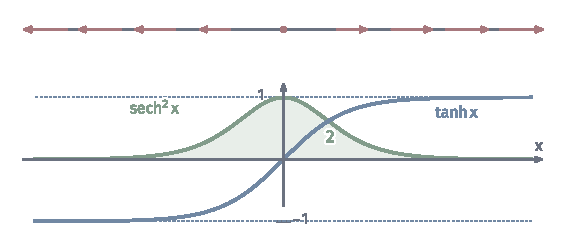
\includegraphics[width=96mm]{figures/04-spaces-measures-and-geometry/04-manifolds/matplotlib/mcalc-noncompact-flux/figure.pdf}
  \caption{$M=\mathbb R$上的$X=\tanh(x)\,\partial_x$。上方的红箭头是向量场本身，两端趋于$\pm\partial_x$。下方绿线是散度$\operatorname{sech}^2x$，浅绿面积为$2$；蓝线是$X$的分量$\tanh x$，它在两端趋于$\pm1$，这两个极限恰是逃向无穷远的流量。}
  \label{fig:mcalc-noncompact-flux}
\end{BookInlineFigure}

问题在于$fX$没有紧支撑。图~\ref{fig:mcalc-noncompact-flux}上方的箭头显示，流量一直流向无穷远，散度的累计$2$由这两股流量解释。非紧情形要使用分部积分，须验证紧支撑，或者验证被积函数衰减得足够快，使截断后边界项的极限为零。

\paragraph{弱导数与场方程的接口}
式~\eqref{eq:mcalc-integration-by-parts}对紧支撑的$f$不含边界项，可以反过来用作定义。第~\ref{chap:smoothing-weak-derivatives}章在欧氏开集上，用与紧支撑试验函数的积分关系定义弱导数。流形上同样可以说：局部可积的向量场$Y$是函数$u$的弱梯度，若对所有紧支撑于$M$内部的光滑向量场$X$，
\begin{equation}
\int_Mu\,\operatorname{div}X\,\mathrm dV_g=-\int_Mg(Y,X)\,\mathrm dV_g .
\label{eq:mcalc-weak-gradient}
\end{equation}
对光滑的$u$，$Y=\operatorname{grad}u$满足这一式；对不光滑的$u$，它在不求导的前提下刻画了“梯度”。

看圆周上的例子。取$S^1$的角度坐标$\theta\in(-\pi,\pi]$，度量$\mathrm d\theta^2$，$u(\theta)=\lvert\theta\rvert$。$u$在$\theta=0$与$\theta=\pm\pi$处有折点，不是$C^1$函数。对周期的光滑函数$X$，在$(-\pi,0)$与$(0,\pi)$上分别分部积分，
\[
\int_{-\pi}^{\pi}\lvert\theta\rvert X'\,\mathrm d\theta=\pi X(\pi)-\pi X(-\pi)-\int_0^\pi X\,\mathrm d\theta+\int_{-\pi}^0X\,\mathrm d\theta .
\]
边界项因$X$的周期性相消，于是$u$有弱梯度$Y=\operatorname{sgn}(\theta)\,\partial_\theta$。在$\theta=0$处，两侧的边界项因$u$连续而相消，所以折点不妨碍弱导数存在；若函数在某点跳跃，这样的项就消不掉，第~\ref{chap:smoothing-weak-derivatives}章已讨论过这种差别。

同理，方程$\Delta_gu=s$的弱形式是：对所有紧支撑的光滑$\varphi$，
\begin{equation}
-\int_Mg(\operatorname{grad}u,\operatorname{grad}\varphi)\,\mathrm dV_g=\int_Ms\varphi\,\mathrm dV_g ,
\label{eq:mcalc-weak-laplace}
\end{equation}
它只要求$u$有一阶弱导数。下一节的Sobolev空间为这些弱形式提供函数类，而弱解的存在、唯一与边值问题可参考\BookChapterRef{chap:elliptic-equations}{卷六第4章“椭圆方程与边值问题”}。

\section{流形上的函数空间}
\label{sec:mcalc-function-spaces}

上一节的弱梯度与弱形式需要一个函数类：函数本身可积到什么程度，弱导数可积到什么程度。欧氏区域上，这由$L^p$与Sobolev空间回答（第~\ref{chap:function-normed-spaces}章与第~\ref{chap:sobolev-spaces}章）。流形上没有全局坐标，但紧流形可以用有限张坐标图覆盖，每张图里都可以借用欧氏的结果。

本节说明怎样把这些空间搬到紧流形上，哪些性质能搬，搬的时候要核对什么。非紧流形放在最后讨论。

\paragraph{$L^p$空间}
第~\ref{sec:mcalc-function-integration}小节已经把黎曼体积做成$M$上的测度$\operatorname{vol}_g$。对$1\leq p<\infty$，定义
\begin{equation}
\lVert u\rVert_{L^p(M,g)}=\Bigl(\int_M\lvert u\rvert^p\,\mathrm dV_g\Bigr)^{1/p},
\label{eq:mcalc-lp-norm}
\end{equation}
$L^p(M,g)$是使其有限的可测函数（几乎处处相等者视为同一元素）组成的空间；$p=\infty$时取本性上确界。这是一般测度空间上的$L^p$空间的特例，所以第~\ref{chap:function-normed-spaces}章的结论直接适用：它是Banach空间，$p=2$时是Hilbert空间。可测向量场$Y$属于$L^p$，指函数$\lVert Y\rVert_g$属于$L^p(M,g)$，这样的向量场同样构成Banach空间。

\begin{theorem}[紧流形上$L^p$与度量的选择无关]
\label{thm:mcalc-lp-metric-independence}
设$M$是紧流形，$g$与$g'$是$M$上的两个黎曼度量，$1\leq p<\infty$。则存在常数$0<c\leq C$，使对所有可测函数$u$，
\begin{equation}
c\,\lVert u\rVert_{L^p(M,g)}\leq\lVert u\rVert_{L^p(M,g')}\leq C\,\lVert u\rVert_{L^p(M,g)}.
\label{eq:mcalc-lp-equivalence}
\end{equation}
因此$L^p(M,g)$与$L^p(M,g')$是同一个函数集合，范数等价。
\end{theorem}

\begin{proof}
在任一坐标图中令$\kappa=\sqrt{\det\bm G'}/\sqrt{\det\bm G}$。由式~\eqref{eq:mcalc-density-change}，换图时分子分母都乘以$\lvert\det\bm A\rvert$，所以$\kappa$是$M$上与坐标无关的函数，并且连续、处处为正，满足$\mathrm dV_{g'}=\kappa\,\mathrm dV_g$。

紧集上的正连续函数有正的最小值$m$和有限的最大值$m'$，于是
\[
m\int\lvert u\rvert^p\,\mathrm dV_g\leq\int\lvert u\rvert^p\,\mathrm dV_{g'}\leq m'\int\lvert u\rvert^p\,\mathrm dV_g .
\]
开$p$次方即得，$c=m^{1/p}$，$C=m'^{1/p}$。
\end{proof}

所以在紧流形上，“$u$属于$L^p$”是一个不依赖度量的性质，度量只影响范数的具体数值。球面的半径变化是这个定理的最简单情形：半径$a$的球面上$\mathrm dV=a^2\,\mathrm dV_{S^2}$，常数$c=C=a^{2/p}$。

\paragraph{Sobolev空间的内在定义}
有了第~\ref{sec:mcalc-integration-by-parts}节的弱梯度，一阶Sobolev空间可以不借坐标定义。设$M$是紧流形（暂设无边界），$1\leq p<\infty$。若$u\in L^p(M,g)$存在弱梯度$Y$且$Y$属于$L^p$，称$u\in W^{1,p}(M)$，记$\operatorname{grad}u=Y$，并取范数
\begin{equation}
\lVert u\rVert_{W^{1,p}}=\Bigl(\lVert u\rVert_{L^p}^p+\bigl\lVert\,\lVert\operatorname{grad}u\rVert_g\bigr\rVert_{L^p}^p\Bigr)^{1/p}.
\label{eq:mcalc-sobolev-norm}
\end{equation}

弱梯度若存在则几乎处处唯一：两个弱梯度之差$Z$满足$\int g(Z,X)\,\mathrm dV_g=0$对所有光滑$X$成立，在每张坐标图中用光滑向量场逼近$Z$的截断，即得$Z=0$几乎处处，这与第~\ref{chap:smoothing-weak-derivatives}章中弱导数唯一性的论证相同。

前面$S^1$上的$u=\lvert\theta\rvert$就在这个空间里。它的弱梯度是$\operatorname{sgn}(\theta)\,\partial_\theta$，其度量长度恒为$1$。对比圆周上的光滑函数$u_0=1+\tfrac12\cos\theta$，它的$W^{1,2}$范数可以直接计算：
\[
\lVert u_0\rVert_{L^2}^2=\int_0^{2\pi}\bigl(1+\tfrac12\cos\theta\bigr)^2\,\mathrm d\theta=\frac94\pi ,\qquad
\lVert u_0'\rVert_{L^2}^2=\frac\pi4 .
\]
两者相加，$\lVert u_0\rVert_{W^{1,2}}^2=\tfrac52\pi$。这里用的是$S^1$的标准度量；下面的定理说明这个空间在选取度量之后的性质。

\begin{theorem}[$W^{1,p}(M)$的完备性]
\label{thm:mcalc-sobolev-complete}
在紧黎曼流形上，$W^{1,p}(M)$是Banach空间。
\end{theorem}

\begin{proof}
设$(u_m)$是$W^{1,p}$中的Cauchy列，则$(u_m)$与$(\operatorname{grad}u_m)$分别是$L^p$函数与$L^p$向量场中的Cauchy列。由$L^p$的完备性，$u_m\to u$，$\operatorname{grad}u_m\to Y$。

对任一光滑向量场$X$，$\operatorname{div}X$与$\lVert X\rVert_g$在紧集$M$上有界，由Hölder不等式，式~\eqref{eq:mcalc-weak-gradient}两端可以取极限：
\[
\begin{aligned}
\int u\,\operatorname{div}X\,\mathrm dV_g&=\lim_m\int u_m\operatorname{div}X\,\mathrm dV_g\\
&=-\lim_m\int g(\operatorname{grad}u_m,X)\,\mathrm dV_g=-\int g(Y,X)\,\mathrm dV_g .
\end{aligned}
\]
所以$Y$是$u$的弱梯度，$u\in W^{1,p}$，并且$u_m\to u$在$W^{1,p}$范数下成立。
\end{proof}

\paragraph{坐标图中的定义与等价性}
内在定义便于理解，计算与证明则常常借助坐标。取有限个坐标图$(U_\alpha,\varphi_\alpha)$，$\alpha=1,\ldots,m$，覆盖$M$，并要求每个$\overline{U_\alpha}$紧，且落在一张更大的坐标图内；紧性保证这样的有限覆盖存在。再取从属的单位分解$\{\psi_\alpha\}$。

对函数$u$，$(\psi_\alpha u)\circ\varphi_\alpha^{-1}$是$\mathbb R^n$上紧支撑的函数，令
\begin{equation}
\lVert u\rVert'_{W^{1,p}}=\sum_{\alpha=1}^m\bigl\lVert(\psi_\alpha u)\circ\varphi_\alpha^{-1}\bigr\rVert_{W^{1,p}(\mathbb R^n)} .
\label{eq:mcalc-chart-sobolev}
\end{equation}
图~\ref{fig:mcalc-chart-cover}在圆周上演示了这个构造：单位分解把$u$切成两段，每段落在一张图的内部，可以在普通的区间上用Sobolev范数度量。

\begin{BookInlineFigure}
  \centering
  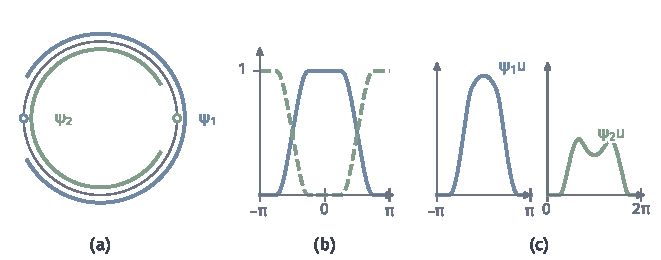
\includegraphics[width=112mm]{figures/04-spaces-measures-and-geometry/04-manifolds/matplotlib/mcalc-chart-cover/figure.pdf}
  \caption{圆周上的有限覆盖与单位分解。(a)两张角度图，分别漏掉$(-1,0)$与$(1,0)$（空心圆），蓝弧与绿弧是$\psi_1,\psi_2$的支撑，每个支撑严格落在所在的图内。(b)$\psi_1$（实线）与$\psi_2=1-\psi_1$（虚线），横轴是角度$\theta$。(c)$u=1+\tfrac12\cos\theta$被切成的两段$\psi_1u$与$\psi_2u$，分别画在各自的图中，都是区间上紧支撑的函数。}
  \label{fig:mcalc-chart-cover}
\end{BookInlineFigure}

在每个$\overline{U_\alpha}$上，度量矩阵的特征值有正的上下界，所以$\lVert\xi\rVert_g$与坐标欧氏长度$\lVert\xi\rVert_2$、$\mathrm dV_g$与$\mathrm d\bm x$在常数倍内可比。单位分解函数及其导数有界，并且乘积规则对弱梯度仍成立：
\[
\operatorname{grad}(\psi_\alpha u)=\psi_\alpha\operatorname{grad}u+u\operatorname{grad}\psi_\alpha .
\]

由这些估计可以得到$\lVert\cdot\rVert'$与$\lVert\cdot\rVert_{W^{1,p}}$等价，并且换用另一组有限覆盖或单位分解只改变等价常数。完整写出常数需要把上面的上下界逐项收集，篇幅较长；结论的含义是，一阶Sobolev空间作为函数集合只取决于光滑结构，度量与覆盖的选择只影响范数的数值。

这一等价性是搬运欧氏结论的通道。例如光滑函数的稠密性：对$u\in W^{1,p}(M)$，把每个$(\psi_\alpha u)\circ\varphi_\alpha^{-1}$用第~\ref{chap:smoothing-weak-derivatives}章的磨光逼近，再拉回求和，得到逼近$u$的光滑函数。磨光后支撑仍落在稍大的坐标域内，这正是要求$\overline{U_\alpha}$落在更大坐标图中的原因。

高阶空间$W^{k,p}(M)$可以同样用坐标图定义，也可以用协变导数$\nabla^ku$内在地定义，两者在紧流形上等价，证明需要逐阶比较协变导数与坐标偏导数，读者可查阅几何分析方面的教材。第~\ref{chap:sobolev-spaces}章的连续嵌入与紧嵌入也可以经有限覆盖搬到紧流形上，所得常数依赖覆盖与度量。

\paragraph{带边界的情形}
紧的带边界流形上，边界附近的坐标图取值于半空间。第~\ref{chap:sobolev-spaces}章在半空间或光滑边界区域上建立的延拓、迹与约束子空间，经边界坐标图搬到流形上，须逐项核对两件事。

一是所用的欧氏结论是否要求边界光滑：流形的边界在定义上光滑，但带角点的区域不在这一框架内。二是结论在坐标变换下是否保持：例如“迹为零”的子空间与坐标无关，而迹的具体范数依赖坐标与度量。Dirichlet条件对应$W^{1,p}$中“迹为零”的闭子空间，Neumann条件则不进入空间的定义，而是在弱形式中由边界项自然体现。

\paragraph{非紧流形}
非紧流形上，有限覆盖不复存在，逐图的控制与整体范数有限是两回事。$\mathbb R$上的常函数$u\equiv1$在每个有界坐标区间上都属于$L^p$与$W^{1,p}$，整体上却不属于$L^p(\mathbb R)$。为区分这两层，记$L^p_{\mathrm{loc}}$与$W^{1,p}_{\mathrm{loc}}$为在每个紧子集上满足相应条件的函数。局部空间不依赖度量，整体空间则依赖度量。

整体空间对度量的依赖在非紧时不再是范数等价那么简单。$\mathbb R$上取$g=\mathrm dx^2$与$g'=(1+x^2)^2\mathrm dx^2$，二者的体积密度之比为$1+x^2$，无界。函数$u(x)=(1+\lvert x\rvert)^{-1}$满足
\[
\int_{\mathbb R}u^2\,\mathrm dx<\infty,\qquad\int_{\mathbb R}u^2(1+x^2)\,\mathrm dx=\infty ,
\]
第二个积分发散是因为被积函数在无穷远处趋于$1$。所以$u\in L^2(\mathbb R,g)$却$u\notin L^2(\mathbb R,g')$，两个空间是不同的集合。

欧氏结论也不能无条件继承。紧流形上$W^{1,2}(M)\hookrightarrow L^2(M)$是紧嵌入；$\mathbb R$上则不然。取支撑含于$(0,1)$的非零光滑函数$\varphi$及其平移$\varphi(x-k)$，$k=1,2,\ldots$，它们在$W^{1,2}(\mathbb R)$中有界，而由于支撑不交，
\[
\lVert\varphi(\cdot-k)-\varphi(\cdot-l)\rVert_{L^2}=\sqrt2\,\lVert\varphi\rVert_{L^2},\qquad k\neq l ,
\]
所以这列函数没有$L^2$收敛的子列。这与第~\ref{chap:functions-as-vectors}章中无限维闭球不紧的现象同源：平移把一个固定的函数送到互不相交的位置，相当于在$L^2$中给出无穷多个互相正交的方向。

非紧流形上嵌入不等式的常数还可能因体积或曲率失去一致的控制而失效，使用时须先核对流形的整体几何条件。

\section{本章小结}
\label{sec:mcalc-summary}

本章开头的问题是：在流形上怎样求导、怎样积分，内部的变化怎样汇总到边界。第一部分只用光滑结构回答。微分形式是对多个切向量的交替读数，楔积按次数满足交换符号规则，拉回沿映射反向作用且对任何光滑映射都有定义，外微分把$k$形式变为$k+1$形式，对函数就是$\mathrm df$，与楔积、拉回相容，并满足$\mathrm d\circ\mathrm d=0$。闭而不恰当的形式，如穿孔平面上的$(x_1\,\mathrm dx_2-x_2\,\mathrm dx_1)/r^2$，反映流形的拓扑。

积分最高次形式还需要定向：形式的系数按带符号的Jacobian行列式变换，只有在定向图册中它才与积分换元公式中的绝对值一致。球面的两张球极投影图要调整一个坐标的符号才构成定向图册，M\"obius带则根本没有定向。边界的诱导定向采用“外法向在前”的约定，在这一约定下，Stokes公式把$\mathrm d\omega$在流形上的积分与$\omega$在边界上的积分联系起来，对紧支撑的$(n-1)$形式成立，紧支撑与定向都不可省略；Green、Gauss与经典Stokes公式是它在平面区域、三维区域与有向曲面上的特例。

第二部分加入黎曼度量。体积密度$\sqrt{\det\bm G}\,\mathrm d\bm x$以Jacobian的绝对值变换，因而不需要定向，在可定向时对应体积形式。由它得到的函数积分是一个测度积分，与定向无关，随度量改变，也不同于样本的采样测度。梯度用度量把$\mathrm df$变成向量，Hessian用Levi-Civita联络扣除方向场的变化，是对称双线性型；散度是协变导数的迹，坐标式只含体积密度；Laplace--Beltrami算子是梯度的散度，在本书约定下非正。球面高度函数把这些运算串在一起：$\operatorname{grad}h$沿经线指向北极，$\operatorname{Hess}h=-hg$，$\Delta h=-2h$，三个结果彼此印证。

梯度、散度与散度定理合成分部积分公式，边界项在闭流形、紧支撑或Dirichlet、Neumann条件下消失，非紧时须另行核对；它也给出弱梯度与场方程弱形式的定义。在紧流形上，有限坐标覆盖、单位分解和黎曼体积把$L^p$与Sobolev空间搬了过来，空间本身不依赖度量的选择，完备性与稠密性得以保留。非紧时须区分局部与整体的控制，欧氏的紧嵌入等结论不能无条件继承。这些运算为后续的流形优化与场方程提供了合法使用的条件。


\chapter{Lie群}
\label{chap:lie-groups}

把一组三维点整体转一个角度，点之间的距离不变，表示朝向的向量却跟着转动。把这组点重新编号，空间中的点一个也没有移动，记录点的矩阵却换了行序。要说清某个计算结果“不受旋转影响”还是“随旋转同步变化”，先要知道允许哪些变换、它们怎样接连施加和撤销、每个变换作用在什么对象上。

另一方面，三维朝向由九个矩阵元素记录，却只有三个自由度。两张旋转矩阵的平均通常不再是旋转矩阵，直接在矩阵元素上做加减会破坏约束。第~\ref{chap:manifold-relations}章告诉我们，旋转矩阵组成一个弯曲的子流形；本章要进一步利用“旋转可以复合”这一事实，在这个弯曲的集合上做计算。

这两类问题都要求把变换的复合规则本身当作研究对象。第~\ref{sec:lie-groups}节用置换、平移和旋转的复合建立群、子群与同态。第~\ref{sec:lie-actions}节规定同一个群怎样作用在不同对象上，用轨道和稳定子描述“能到哪里”和“哪些变换不起作用”，再定义不变映射与等变映射。

旋转可以连续地变化，所以第~\ref{sec:lie-matrix-groups}节把矩阵群看成流形：单位元处的切空间即Lie代数，记录无穷小变化，矩阵指数把这些方向变回群中的变换。第~\ref{sec:lie-rotations}节围绕同一个三维旋转比较旋转矩阵、轴角与单位四元数，第~\ref{sec:lie-rigid-poses}节加入平移，建立刚体位姿的计算规则。

最后，第~\ref{sec:lie-quotients}节处理“多种记录代表同一对象”的问题：用群作用把等价的记录合并，说明何时得到光滑的商流形，并建立射影空间与Grassmann空间。

本章依赖第~\ref{chap:manifold-basics}章的流形与切空间、第~\ref{chap:manifold-maps}章的光滑映射与微分、第~\ref{chap:manifold-relations}章的正则水平集，以及第~\ref{chap:topological-spaces}章的商拓扑。由对应点实际估计旋转、平移和射影变换是第~\ref{chap:spatial-map-estimation}章的任务；正交矩阵与子空间约束下的优化算法见\BookChapterRef{chap:manifold-optimization}{卷五第12章“流形约束下的优化”}。

\section{群}
\label{sec:lie-groups}

重新排列三个物品的位置、把平面整体平移一段距离、把平面绕原点转一个角度，这三类操作作用的对象各不相同，却遵循同样的规则：两个操作可以接连施加，得到的仍是同类操作；“什么都不做”也算一个操作；每个操作都可以撤销。本节先把这些规则从具体对象中抽出来，建立群、子群与同态。这里只固定变换之间怎样复合，同一个群怎样作用在不同对象上留给第~\ref{sec:lie-actions}节，这样就不会把一个群只理解成某一套坐标矩阵。

\subsection{群与子群}
\label{sec:lie-group-subgroup}

本小节先从置换的复合读出群公理，再看几类基本例子和反例，最后研究限制允许变换得到的子群。

\paragraph{从变换的复合到群公理}
先看集合$\{1,2,3\}$上的置换，即从这个集合到自身的双射。置换$\sigma$交换$1$与$2$、保持$3$不动，置换$\tau$交换$2$与$3$、保持$1$不动。复合$\sigma\circ\tau$表示先做$\tau$、再做$\sigma$：
\[
(\sigma\circ\tau)(1)=\sigma(1)=2,\qquad
(\sigma\circ\tau)(2)=\sigma(3)=3,\qquad
(\sigma\circ\tau)(3)=\sigma(2)=1.
\]
反过来先做$\sigma$再做$\tau$，得到$1\mapsto3$、$2\mapsto1$、$3\mapsto2$。两个结果不同，所以复合的次序必须写清。

这个例子已经包含群的全部要素。两个置换的复合仍是置换；恒等置换$\operatorname{id}$不改变任何元素；每个置换都有逆置换，把它的效果撤销；映射的复合满足结合律$(\alpha\circ\beta)\circ\gamma=\alpha\circ(\beta\circ\gamma)$，因为两边在每个元素上都等于$\alpha(\beta(\gamma(i)))$。平面上的平移$\bm x\mapsto\bm x+\bm a$和绕原点的旋转同样满足这四条，只是平移的复合对应向量相加，旋转的复合对应转角相加。

\begin{definition}[群]
\label{def:lie-group}
设$G$是集合，$G\times G\to G$，$(g,h)\mapsto gh$是$G$上的二元运算。若
\begin{enumerate}
 \item 对所有$g,h,k\in G$，$(gh)k=g(hk)$；
 \item 存在$e\in G$，使对所有$g\in G$，$eg=ge=g$；
 \item 对每个$g\in G$，存在$g^{-1}\in G$，使$gg^{-1}=g^{-1}g=e$，
\end{enumerate}
就称$G$连同这个运算构成\term{群}（group），$e$称为单位元，$g^{-1}$称为$g$的逆元。若还对所有$g,h$有$gh=hg$，就称$G$为\term{交换群}（commutative group）。
\end{definition}

运算“封闭”已经写在$G\times G\to G$之中：乘积必须仍在$G$里。乘法记号$gh$只是约定，它可以是映射的复合、数的加法或矩阵乘法。对由变换组成的群，本章总按复合约定$gh=g\circ h$，即先做$h$、再做$g$。

\paragraph{几个基本例子}
$\{1,\ldots,n\}$上全部置换在复合下构成群，称为\term{对称群}（symmetric group），记为$S_n$，它有$n!$个元素。上面的计算说明$S_3$不是交换群。$\mathbb R^d$在向量加法下构成交换群，单位元是$\bm0$，逆元是$-\bm a$；它记录平面或空间中的全部平移。

平面旋转由矩阵
\begin{equation}
 \bm R(\theta)=\begin{bmatrix}\cos\theta&-\sin\theta\\\sin\theta&\cos\theta\end{bmatrix}
 \label{eq:lie-planar-rotation}
\end{equation}
表示。由和角公式，$\bm R(\theta_1)\bm R(\theta_2)=\bm R(\theta_1+\theta_2)$，所以平面旋转的复合与次序无关，单位元是$\bm R(0)=\bm I$，逆元是$\bm R(-\theta)=\bm R(\theta)^\top$。

更一般的矩阵例子如下。全体$n$阶可逆实矩阵在矩阵乘法下构成\term{一般线性群}（general linear group），记为$\mathrm{GL}(n,\mathbb R)$。满足$\bm Q^\top\bm Q=\bm I$的正交矩阵构成\term{正交群}（orthogonal group）$\mathrm O(n)$：若$\bm Q_1,\bm Q_2$正交，则$(\bm Q_1\bm Q_2)^\top\bm Q_1\bm Q_2=\bm Q_2^\top\bm Q_2=\bm I$，且$\bm Q^{-1}=\bm Q^\top$仍正交。正交矩阵的行列式为$\pm1$，其中行列式为$1$的构成\term{特殊正交群}（special orthogonal group）$\mathrm{SO}(n)$。当$n=2$时，$\mathrm{SO}(2)$恰由式~\eqref{eq:lie-planar-rotation}中的矩阵组成：第一列$(a,b)^\top$是单位向量，第二列与它正交且使行列式为$1$，只能是$(-b,a)^\top$，再记$a=\cos\theta$、$b=\sin\theta$即可。

\paragraph{不构成群的情形}
公理中的每一条都会实际排除一些对象。全体$n$阶实矩阵在乘法下不是群，因为奇异矩阵没有逆；把一个向量投影到某条直线上的操作不可撤销，同样不能放进群里。整数在减法下不是群，因为$(1-2)-3\neq1-(2-3)$，结合律失败。若一组图像增强操作接连施加后不再属于这一组，运算不封闭，也不能直接称为群。

单位元和逆元一旦存在就是唯一的，因此记号$e$与$g^{-1}$没有歧义。

\begin{lemma}[单位元与逆元的唯一性]
\label{lem:lie-identity-inverse-unique}
群$G$中单位元唯一；每个$g\in G$的逆元唯一。并且对任意$g,h\in G$，$(gh)^{-1}=h^{-1}g^{-1}$。
\end{lemma}

\begin{proof}
若$e,e'$都是单位元，则$e=ee'=e'$。若$h,h'$都是$g$的逆元，则$h=he=h(gh')=(hg)h'=eh'=h'$。最后，由结合律，$(gh)(h^{-1}g^{-1})=g(hh^{-1})g^{-1}=gg^{-1}=e$，另一侧同理，所以$h^{-1}g^{-1}$是$gh$的逆元。
\end{proof}

最后一式的次序与直觉一致：先穿袜子再穿鞋，撤销时要先脱鞋再脱袜子。对矩阵而言，这就是$(\bm A\bm B)^{-1}=\bm B^{-1}\bm A^{-1}$。

\paragraph{子群}
许多问题只允许一部分变换。例如只允许转$90^\circ$的整数倍，或只允许沿水平方向平移。这些变换自身仍然能复合和撤销，于是在原来的群中又形成一个群。

\begin{definition}[子群]
\label{def:lie-subgroup}
设$G$是群，$H\subseteq G$。若$e\in H$，并且对任意$g,h\in H$都有$gh\in H$与$g^{-1}\in H$，就称$H$是$G$的\term{子群}（subgroup）。
\end{definition}

子群继承了原来的运算，结合律自动成立，所以它本身是群。验证子群时，常把三个条件合成一条。

\begin{lemma}[子群判别]
\label{lem:lie-subgroup-criterion}
群$G$的非空子集$H$是子群，当且仅当对任意$g,h\in H$都有$gh^{-1}\in H$。
\end{lemma}

\begin{proof}
必要性由定义直接得到。反过来，取$g\in H$，令$h=g$得$e=gg^{-1}\in H$；再取第一个元素为$e$，得$h^{-1}=eh^{-1}\in H$；最后对$g,h\in H$，由$h^{-1}\in H$得$gh=g(h^{-1})^{-1}\in H$。
\end{proof}

转$90^\circ$整数倍的旋转$\{\bm R(k\pi/2):k=0,1,2,3\}$是$\mathrm{SO}(2)$的子群，它只有四个元素。水平平移$\{(a,0)^\top:a\in\mathbb R\}$是$\mathbb R^2$的子群。矩阵群之间有包含链$\mathrm{SO}(n)\subseteq\mathrm O(n)\subseteq\mathrm{GL}(n,\mathbb R)$，每一个都是后一个的子群。

\paragraph{子集与子群的区别}
子群是“允许的变换”组成的子集，并且对群运算封闭；它不同于被变换对象的一个子集，也不同于群的任意子集。在平移群$\mathbb R^2$中，单位圆$\{\bm x:\lVert\bm x\rVert_2=1\}$是一个子集，却不是子群：$(1,0)^\top+(1,0)^\top=(2,0)^\top$不在圆上，零向量也不在圆上。

同样，$\mathrm O(n)$中行列式为$-1$的矩阵（反射类变换）组成的子集不是子群：它不含$\bm I$，两个反射的乘积行列式为$1$，又回到了旋转。可见“满足某个条件的变换”能否形成子群，要逐条核对单位元、乘积和逆元，不能只看条件写起来是否自然。

\subsection{群同态}
\label{sec:lie-homomorphism}

同一套变换规则可以用不同方式记录。平面旋转可以用转角$\theta$记录，也可以用矩阵$\bm R(\theta)$记录；三个物品的置换可以写成映射表，也可以写成置换矩阵。要说明两种记录描述的是同一个复合结构，需要一个保持复合的映射。

\begin{definition}[群同态与同构]
\label{def:lie-homomorphism}
设$G,H$是群。映射$\varphi:G\to H$若对所有$g_1,g_2\in G$满足
\begin{equation}
 \varphi(g_1g_2)=\varphi(g_1)\varphi(g_2),
 \label{eq:lie-homomorphism}
\end{equation}
就称为\term{群同态}（group homomorphism）。双射的群同态称为\term{群同构}（group isomorphism）。同态的\term{核}（kernel）是$\ker\varphi=\{g\in G:\varphi(g)=e_H\}$，像是$\varphi(G)=\{\varphi(g):g\in G\}$。
\end{definition}

式~\eqref{eq:lie-homomorphism}左边先在$G$中复合再映过去，右边先映过去再在$H$中复合，二者相等。由$\varphi(e_G)=\varphi(e_Ge_G)=\varphi(e_G)\varphi(e_G)$，两边左乘$\varphi(e_G)^{-1}$得$\varphi(e_G)=e_H$；再由$\varphi(g)\varphi(g^{-1})=\varphi(e_G)=e_H$得$\varphi(g^{-1})=\varphi(g)^{-1}$。所以同态自动保持单位元与逆元。

\paragraph{同态的例子}
由式~\eqref{eq:lie-planar-rotation}定义的$\theta\mapsto\bm R(\theta)$是从加法群$\mathbb R$到$\mathrm{SO}(2)$的同态，因为$\bm R(\theta_1+\theta_2)=\bm R(\theta_1)\bm R(\theta_2)$。它是满射，核为$\{2\pi k:k\in\mathbb Z\}$：转角相差$2\pi$的整数倍，得到同一个旋转。

行列式给出同态$\det:\mathrm{GL}(n,\mathbb R)\to\mathbb R\setminus\{0\}$，后者取数的乘法，因为$\det(\bm A\bm B)=\det\bm A\det\bm B$。它的核是行列式为$1$的矩阵全体，记为$\mathrm{SL}(n,\mathbb R)$。

对$\pi\in S_n$，令置换矩阵$\bm P_\pi$的第$j$列为$\bm e_{\pi(j)}$，即$\bm P_\pi\bm e_j=\bm e_{\pi(j)}$。于是
\[
\bm P_{\pi_1}\bm P_{\pi_2}\bm e_j=\bm P_{\pi_1}\bm e_{\pi_2(j)}=\bm e_{\pi_1(\pi_2(j))}=\bm P_{\pi_1\pi_2}\bm e_j,
\]
所以$\pi\mapsto\bm P_\pi$是从$S_n$到$\mathrm{GL}(n,\mathbb R)$的同态，像落在$\mathrm O(n)$中。不同置换给出不同矩阵，这个同态是单射。

把群的复合规则落实为可逆线性映射，是比较各种表示时最常用的同态，下面单独命名。

\begin{definition}[线性表示]
\label{def:lie-linear-representation}
设$G$是群，$V$是有限维实向量空间，$\mathrm{GL}(V)$是$V$上全部可逆线性映射在复合下构成的群。群同态$\rho:G\to\mathrm{GL}(V)$称为$G$在$V$上的\term{线性表示}（linear representation）。
\end{definition}

同一个群可以有许多线性表示。$\mathrm{SO}(2)$可以按$\rho(\bm R)=\bm R$作用在$\mathbb R^2$上，也可以按$\rho(\bm R)=1$作用在$\mathbb R$上，后者把每个旋转都表示为“不做任何事”。第~\ref{sec:lie-invariant-equivariant}节会用这两种表示区分不变与等变。

\paragraph{核与像保留什么}
核记录同态把哪些元素“看成单位元”，因而丢失了哪些区分；像记录目标群中有哪些元素被实际表示出来。下面的结论说明，核只含单位元时同态不丢失任何区分。

\begin{theorem}[核与单射]
\label{thm:lie-kernel-injective}
设$\varphi:G\to H$是群同态。则$\ker\varphi$是$G$的子群，$\varphi(G)$是$H$的子群，并且$\varphi(g_1)=\varphi(g_2)$当且仅当$g_1^{-1}g_2\in\ker\varphi$。特别地，$\varphi$是单射当且仅当$\ker\varphi=\{e_G\}$。
\end{theorem}

\begin{proof}
若$g,h\in\ker\varphi$，则$\varphi(gh^{-1})=\varphi(g)\varphi(h)^{-1}=e_H$，由引理~\ref{lem:lie-subgroup-criterion}知核是子群；对像中的$\varphi(g),\varphi(h)$，有$\varphi(g)\varphi(h)^{-1}=\varphi(gh^{-1})$仍在像中，所以像也是子群。其次，$\varphi(g_1)=\varphi(g_2)$等价于$e_H=\varphi(g_1)^{-1}\varphi(g_2)=\varphi(g_1^{-1}g_2)$，即$g_1^{-1}g_2\in\ker\varphi$。最后，若核只含$e_G$，则$\varphi(g_1)=\varphi(g_2)$推出$g_1^{-1}g_2=e_G$，即$g_1=g_2$；反之，单射把$e_G$之外的元素都映到$e_H$之外。
\end{proof}

回到转角的例子：$\varphi(\theta)=\bm R(\theta)$的核是$2\pi\mathbb Z$，所以$\bm R(\theta_1)=\bm R(\theta_2)$当且仅当$\theta_2-\theta_1\in2\pi\mathbb Z$。转角能完整记录旋转的复合，却在每个旋转上多出可数个等价的记录；第~\ref{sec:lie-rotations}节的轴角与四元数会遇到同类的冗余。

\paragraph{结构对应与集合对应}
两个群元素个数相同，只说明它们之间有集合层面的双射，不说明复合规则相同。$S_3$有$6$个元素，$\{0,1,\ldots,5\}$在模$6$加法下也构成$6$个元素的群，二者之间当然有双射。但模$6$加法群是交换群，$S_3$不是；若$\varphi$是同构，则$\varphi(\sigma)\varphi(\tau)=\varphi(\tau)\varphi(\sigma)$，由单射性得$\sigma\tau=\tau\sigma$，与本节开头的计算矛盾。所以这两个群不同构。

另一方面，平面旋转$\bm R(\theta)$与单位圆上的点$(\cos\theta,\sin\theta)^\top$一一对应。只有给单位圆指定运算，例如把点看成单位复数$e^{\mathrm i\theta}$并取复数乘法，这个对应才成为群同构。判断两种记录是否表达同一个变换结构，要检查的是复合规则是否被保持，而不只是元素能否配对。

\section{群作用}
\label{sec:lie-actions}

上一节的群只规定了变换之间怎样复合。同一个旋转可以转动一个点、一整组点，也可以转动一幅定义在平面上的图像；被变换的对象不同，计算公式也不同。本节先规定群元素怎样作用在给定集合上，并核对作用与复合相容；再用轨道与稳定子描述对象之间通过变换建立的关系；最后在输入与输出的作用都给定后，说明映射的结果应怎样随输入变换。

\begin{definition}[群作用]
\label{def:lie-group-action}
设$G$是群，$X$是集合。映射$G\times X\to X$，$(g,x)\mapsto g\cdot x$若满足
\begin{equation}
 e\cdot x=x,\qquad (g_1g_2)\cdot x=g_1\cdot(g_2\cdot x)\qquad(g_1,g_2\in G,\ x\in X),
 \label{eq:lie-group-action}
\end{equation}
就称为$G$在$X$上的\term{群作用}（group action）。
\end{definition}

第一条说单位元什么也不做，第二条说先用$g_2$作用、再用$g_1$作用，与用乘积$g_1g_2$作用一次相同。对固定的$g$，映射$x\mapsto g\cdot x$有逆映射$x\mapsto g^{-1}\cdot x$，因为$g^{-1}\cdot(g\cdot x)=(g^{-1}g)\cdot x=x$。所以群作用相当于一个同态，把每个$g$对应为$X$上的一个双射。

\paragraph{同一个群在不同对象上的作用}
$\mathrm{SO}(2)$在$\mathbb R^2$上按矩阵乘法$\bm R\cdot\bm x=\bm R\bm x$作用，两条规则就是$\bm I\bm x=\bm x$与矩阵乘法的结合律。$\mathbb R^2$也按$\bm a\cdot\bm x=\bm x+\bm a$作用在自身上。

点云由$n$个点组成，记为$\bm X\in\mathbb R^{n\times D}$，第$i$行$\bm X_{i,:}$是第$i$个点的坐标。$S_n$按$\pi\cdot\bm X=\bm P_\pi\bm X$作用，其中$\bm P_\pi$沿用上一节的置换矩阵；由$\bm P_\pi\bm e_j=\bm e_{\pi(j)}$可以算出$(\bm P_\pi\bm X)_{i,:}=\bm X_{\pi^{-1}(i),:}$，即原来的第$j$行被搬到第$\pi(j)$行。$\mathrm{SO}(D)$则按$\bm R\cdot\bm X=\bm X\bm R^\top$作用，把每一行$\bm x^\top$变成$(\bm R\bm x)^\top$。两种作用都写成矩阵乘法，前者改变点的编号，后者移动点的位置，被改变的对象和索引完全不同。

旋转还可以作用在平面图像上。把图像记为函数$f:\mathbb R^2\to\mathbb R$，令
\[
(\bm R\cdot f)(\bm x)=f(\bm R^{-1}\bm x).
\]
这里必须用$\bm R^{-1}$：新图像在$\bm x$处的值，来自旧图像中转到$\bm x$之前的位置。验证第二条规则：$(\bm R_1\cdot(\bm R_2\cdot f))(\bm x)=(\bm R_2\cdot f)(\bm R_1^{-1}\bm x)=f(\bm R_2^{-1}\bm R_1^{-1}\bm x)=f((\bm R_1\bm R_2)^{-1}\bm x)$，恰为$((\bm R_1\bm R_2)\cdot f)(\bm x)$。若改写成$f(\bm R\bm x)$，复合次序就会颠倒，在非交换群上不再满足式~\eqref{eq:lie-group-action}。

\subsection{轨道与稳定子}
\label{sec:lie-orbits-stabilizers}

给定作用后，可以问两个方向相反的问题：从一个对象出发，经过群中的变换能到达哪些对象；哪些变换根本不改变这个对象。前者给出轨道，后者给出稳定子。

\begin{definition}[轨道与稳定子]
\label{def:lie-orbit-stabilizer}
设群$G$作用于$X$，$x\in X$。称
\[
G\cdot x=\{g\cdot x:g\in G\},\qquad G_x=\{g\in G:g\cdot x=x\}
\]
分别为$x$的\term{轨道}（orbit）与\term{稳定子}（stabilizer）。若$X$只有一条轨道，就称作用是\term{传递作用}（transitive action）。
\end{definition}

轨道是$X$的子集，稳定子是$G$的子集，二者不在同一个空间里。规定$x\sim y$当且仅当存在$g\in G$使$y=g\cdot x$。单位元给出$x\sim x$；若$y=g\cdot x$，则$x=g^{-1}\cdot y$，给出对称性；若$y=g\cdot x$、$z=h\cdot y$，则$z=(hg)\cdot x$，给出传递性。所以$\sim$是等价关系，其等价类恰是轨道。由等价关系与划分的对应（可参考\BookChapterRef{chap:sets-relations-maps}{卷一第1章“集合、关系与映射”}），不同的轨道互不相交，且所有轨道的并是$X$。轨道组成的商集记为$X/G$。

稳定子则总是子群。若$g,h\in G_x$，则$h^{-1}\cdot x=h^{-1}\cdot(h\cdot x)=x$，于是$(gh^{-1})\cdot x=g\cdot(h^{-1}\cdot x)=x$，由引理~\ref{lem:lie-subgroup-criterion}得$G_x$是子群。

\paragraph{旋转作用的轨道}
$\mathrm{SO}(2)$作用于$\mathbb R^2$时，$\bm x\neq\bm0$的轨道是半径为$\lVert\bm x\rVert_2$的圆：旋转保持长度，并且同一圆上任意两点之间都有一个旋转把一点送到另一点。原点的轨道只有原点自身。非零点的稳定子只含$\bm I$，原点的稳定子是整个$\mathrm{SO}(2)$。轨道可以用半径$r\geq0$编号，所以$\mathbb R^2/\mathrm{SO}(2)$可以识别为$[0,\infty)$，原点的轨道对应端点$0$。

$\mathrm{SO}(3)$作用于$\mathbb R^3$时，非零点的轨道是球面。以$\bm e_3=(0,0,1)^\top$为例，它的轨道是单位球面$S^2$，稳定子是绕第三坐标轴的全部旋转
\[
\left\{\begin{bmatrix}\bm R(\theta)&\bm0\\\bm0^\top&1\end{bmatrix}:\theta\in\mathbb R\right\},
\]
这是一个与$\mathrm{SO}(2)$同构的子群。这里有三个不同的空间：群$\mathrm{SO}(3)$由旋转组成，单个对象$\bm e_3$是一个点，轨道$S^2$是一个曲面。许多不同的旋转把$\bm e_3$送到同一个点，所以不能把$\mathrm{SO}(3)$与球面$S^2$等同；第~\ref{sec:lie-quotients}节会说明$S^2$正是$\mathrm{SO}(3)$按这个稳定子取商的结果。

\paragraph{轨道与陪集}
两个变换把$x$送到同一个点，当且仅当它们只差一个稳定子中的元素：$g\cdot x=h\cdot x$等价于$(h^{-1}g)\cdot x=x$，即$h^{-1}g\in G_x$。为了记录“只差$G_x$中元素”的变换，引入下面的集合。

\begin{definition}[陪集]
\label{def:lie-coset}
设$H$是群$G$的子群，$g\in G$。称$gH=\{gh:h\in H\}$为$H$的一个左\term{陪集}（coset）。全体左陪集组成的集合记为$G/H$。
\end{definition}

$h^{-1}g\in G_x$恰等价于$g\in hG_x$，于是$gG_x=hG_x$当且仅当$g\cdot x=h\cdot x$。这说明映射$gG_x\mapsto g\cdot x$不依赖代表元，并且是从$G/G_x$到轨道$G\cdot x$的双射。

\begin{theorem}[轨道—稳定子关系]
\label{thm:lie-orbit-stabilizer}
设群$G$作用于$X$，$x\in X$。则$gG_x\mapsto g\cdot x$是$G/G_x$到$G\cdot x$的双射。若$G$是有限群，则$\lvert G\cdot x\rvert\,\lvert G_x\rvert=\lvert G\rvert$。
\end{theorem}

\begin{proof}
双射已在上一段证明。有限情形下，左乘$g$是$G$到自身的双射，把$G_x$一一地映成$gG_x$，所以每个陪集都有$\lvert G_x\rvert$个元素。不同陪集互不相交：若$k\in gG_x\cap hG_x$，则$k\cdot x=g\cdot x=h\cdot x$，从而$gG_x=hG_x$。每个$g$都在自己的陪集$gG_x$中，所以$G$被分成$\lvert G/G_x\rvert=\lvert G\cdot x\rvert$个大小为$\lvert G_x\rvert$的块。
\end{proof}

用$S_3$作用于$\{1,2,3\}$核对：$1$的轨道是$\{1,2,3\}$，稳定子是$\{\operatorname{id},\tau\}$，其中$\tau$交换$2$与$3$，确有$3\times2=6$。对点云，若$\bm X$的$n$行互不相同，则只有恒等置换保持$\bm X$，轨道有$n!$个元素，对应同一组点的$n!$种编号方式；若恰有两行相同，交换这两行也保持$\bm X$，稳定子有$2$个元素，轨道只有$n!/2$个不同的矩阵。

\subsection{不变映射与等变映射}
\label{sec:lie-invariant-equivariant}

在点云上计算一个量时，任务往往对变换有明确要求。点的重新编号不应改变“这组点的重心在哪里”；整体旋转之后，重心应跟着转到新的位置，而点之间的距离则不应改变。两种要求都是在比较“变换后再计算”与“计算后再变换”，区别在于输出是否也受到作用。

\begin{definition}[不变映射与等变映射]
\label{def:lie-invariant-equivariant}
设群$G$作用于$X$与$Y$，映射$f:X\to Z$，$F:X\to Y$。若
\begin{equation}
 f(g\cdot x)=f(x)\qquad(g\in G,\ x\in X),
 \label{eq:lie-invariant}
\end{equation}
就称$f$是\term{不变映射}（invariant map）。若
\begin{equation}
 F(g\cdot x)=g\cdot F(x)\qquad(g\in G,\ x\in X),
 \label{eq:lie-equivariant}
\end{equation}
就称$F$是\term{等变映射}（equivariant map），其中左边的点是$X$上的作用，右边的点是$Y$上的作用。
\end{definition}

不变性只需要输入的作用；等变性必须同时给定输入与输出的作用，否则式~\eqref{eq:lie-equivariant}没有意义。若$Y$上的作用是平凡作用$g\cdot y=y$，等变就退化为不变。所以不变是等变的特例，而不是另一种更强或更好的要求。

\paragraph{同一次变换下的核对}
取$\bm x=(1.3,0.5)^\top$，绕原点逆时针转$90^\circ$，$\bm R(\pi/2)\bm x=(-0.5,1.3)^\top$。长度$f(\bm x)=\lVert\bm x\rVert_2$在变换前后都等于$\sqrt{1.94}$，满足式~\eqref{eq:lie-invariant}。恒等映射$F(\bm x)=\bm x$满足$F(\bm R\bm x)=\bm R\bm x=\bm R F(\bm x)$，是等变映射，但$F(\bm R\bm x)=(-0.5,1.3)^\top\neq F(\bm x)$，所以它不是不变映射。等变保留的是“输出随输入同步变化”的规则，而不是输出保持不动。

\paragraph{点云上的例子}
对点云$\bm X\in\mathbb R^{n\times D}$，令$\bm 1\in\mathbb R^n$为全一向量，重心为$\bm m(\bm X)=\frac1n\bm X^\top\bm 1\in\mathbb R^D$。重新编号时，$\bm m(\bm P_\pi\bm X)=\frac1n\bm X^\top\bm P_\pi^\top\bm 1=\bm m(\bm X)$，因为置换矩阵的每一行恰有一个$1$，$\bm P_\pi^\top\bm 1=\bm 1$。旋转时，$\bm m(\bm X\bm R^\top)=\frac1n\bm R\bm X^\top\bm 1=\bm R\,\bm m(\bm X)$。所以重心对置换不变，对旋转等变，输出的旋转作用是$\bm y\mapsto\bm R\bm y$。

两两距离矩阵$\bm D(\bm X)_{i,j}=\lVert\bm X_{i,:}-\bm X_{j,:}\rVert_2$对旋转不变，因为旋转保持差向量的长度。它对置换却不是不变的：重新编号后，$\bm D(\bm P_\pi\bm X)$的$(i,j)$元是原来第$\pi^{-1}(i)$、$\pi^{-1}(j)$两点的距离，即$\bm D(\bm P_\pi\bm X)=\bm P_\pi\bm D(\bm X)\bm P_\pi^\top$。若在矩阵空间上规定作用$\pi\cdot\bm M=\bm P_\pi\bm M\bm P_\pi^\top$，$\bm D$就是等变的。同一个映射是否“对置换不变”，取决于问的是哪一种输出作用。

\paragraph{不变映射与轨道}
不变映射在同一条轨道上取相同的值，所以它只依赖输入所在的轨道。记$q:X\to X/G$为$q(x)=G\cdot x$，令$\widetilde f(G\cdot x)=f(x)$；若$G\cdot x=G\cdot y$，则$y=g\cdot x$，由不变性$f(y)=f(x)$，所以$\widetilde f$不依赖代表元，并且$f=\widetilde f\circ q$。不变映射正是忽略了同一轨道内的差别。

这种忽略可能过多。$f$可以把不同的轨道映到同一个值，例如把每个点云都映到零的常值映射对一切作用都不变，却不区分任何点云。不变性只说明$f$没有利用轨道内的差别，不说明$f$保留了区分不同轨道所需的信息。

\paragraph{复合与汇总}
等变映射之后接不变映射，结果不变：若$F$等变、$f$在$Y$上不变，则$f(F(g\cdot x))=f(g\cdot F(x))=f(F(x))$。两个等变映射的复合仍等变，理由相同。例如对每个点使用同一个映射$\phi:\mathbb R^D\to\mathbb R^r$，令$\Phi(\bm X)_{i,:}=\phi(\bm X_{i,:})$，则$\Phi(\bm P_\pi\bm X)_{i,:}=\phi(\bm X_{\pi^{-1}(i),:})=(\bm P_\pi\Phi(\bm X))_{i,:}$，所以$\Phi$对置换等变；再对行求和，重新编号只改变求和次序，得到不变的$\sum_i\phi(\bm X_{i,:})$。反过来，若中间已经求和，丢掉了每个点的编号，后面就不能再恢复逐点的等变输出。

\section{矩阵Lie群}
\label{sec:lie-matrix-groups}

置换群只有有限个元素，旋转却可以连续地变化：转角从$0$逐渐增大，旋转矩阵也随之连续变化。对这类群，可以问“单位元附近有哪些变化方向”，也可以要求群运算与这些方向的计算相容。本节先说明矩阵群怎样成为流形，并且乘法与求逆都是光滑映射；再用单位元处的切空间记录无穷小变化，即Lie代数；最后用矩阵指数把Lie代数中的方向变回群中的变换。

\begin{definition}[Lie群]
\label{def:lie-lie-group}
若群$G$同时是光滑流形，并且乘法$G\times G\to G$，$(g,h)\mapsto gh$与求逆$G\to G$，$g\mapsto g^{-1}$都是光滑映射，就称$G$为\term{Lie群}（Lie group）。
\end{definition}

定义要求群结构与光滑结构相容，而不只是“元素可以连续变化”。并非每个由连续变换组成的群都是有限维Lie群。例如以有理数倍$2\pi$为转角的旋转$\{\bm R(2\pi q):q\in\mathbb Q\}$是$\mathrm{SO}(2)$的子群，但它只有可数个元素，并且在单位圆上稠密：任意小的弧内都有它的元素。在继承的拓扑下，它的任一点附近既不像一段开区间，也不是孤立点，因而不是流形。圆周上全体同胚组成的群虽然也由连续变换组成，却不能用有限个实数参数局部描述，超出了本章讨论的范围。

本章只讨论矩阵组成的Lie群。称$\mathrm{GL}(n,\mathbb R)$的子群$G$为\term{矩阵Lie群}（matrix Lie group），若$G$在$\mathrm{GL}(n,\mathbb R)$中是闭集。可以证明，$\mathrm{GL}(n,\mathbb R)$的每个闭子群都是嵌入子流形，从而是Lie群（Cartan闭子群定理），这里不给出证明，可参考\scite{math-lee2013smooth}。下面用到的群都直接验证其流形结构，不依赖这个定理。上面的有理转角子群不是闭集，正好被这一定义排除。

\subsection{光滑结构}
\label{sec:lie-smooth-structure}

要把矩阵群当作流形，需要逐一说明它在矩阵空间中是什么样的子集、乘法与求逆为何光滑，以及各点的切空间怎样联系起来。下面依次处理一般线性群、正交群与左平移。

\paragraph{一般线性群}
把$n$阶实矩阵的$n^2$个元素排成一列，$\mathbb R^{n\times n}$就是欧氏空间。行列式是矩阵元素的多项式，因而连续，所以$\mathrm{GL}(n,\mathbb R)=\{\bm A:\det\bm A\neq0\}$是$\mathbb R^{n\times n}$中的开集，从而是$n^2$维流形，一张坐标图就覆盖全体。矩阵乘积的每个元素是两个因子元素的二次多项式，所以乘法光滑。由古典伴随公式$\bm A^{-1}=\operatorname{adj}(\bm A)/\det\bm A$，逆矩阵的元素是矩阵元素的有理函数，分母$\det\bm A$在$\mathrm{GL}(n,\mathbb R)$上不为零，所以求逆光滑。于是$\mathrm{GL}(n,\mathbb R)$是Lie群。

\paragraph{正交群}
正交群由约束$\bm A^\top\bm A=\bm I$给出。用第~\ref{chap:manifold-relations}章的正则水平集判断它是否是子流形时，约束映射的取值空间要选对。令$\mathrm{Sym}(n)$为$n$阶实对称矩阵组成的空间，维数为$n(n+1)/2$，定义
\[
\Phi:\mathrm{GL}(n,\mathbb R)\to\mathrm{Sym}(n),\qquad \Phi(\bm A)=\bm A^\top\bm A.
\]
$\bm A^\top\bm A$本来就对称，若把$\Phi$看成取值于$\mathbb R^{n\times n}$，上三角与下三角的方程会重复，微分不可能满秩。取值于$\mathrm{Sym}(n)$后，$\mathrm O(n)=\Phi^{-1}(\bm I)$。

\begin{theorem}[正交群的流形结构]
\label{thm:lie-orthogonal-group-manifold}
$\mathrm O(n)$是$\mathrm{GL}(n,\mathbb R)$中$n(n-1)/2$维的嵌入子流形，并且对$\bm A\in\mathrm O(n)$，
\begin{equation}
 T_{\bm A}\mathrm O(n)=\{\bm A\bm\Omega:\bm\Omega^\top=-\bm\Omega\}.
 \label{eq:lie-orthogonal-tangent}
\end{equation}
$\mathrm{SO}(n)$是$\mathrm O(n)$中的开子集，具有相同的维数与切空间。
\end{theorem}

\begin{proof}
沿方向$\bm H$求导，$\mathrm d\Phi_{\bm A}(\bm H)=\bm A^\top\bm H+\bm H^\top\bm A$。设$\bm A\in\mathrm O(n)$，任给$\bm S\in\mathrm{Sym}(n)$，取$\bm H=\frac12\bm A\bm S$，则
\[
\mathrm d\Phi_{\bm A}(\bm H)=\tfrac12\bm A^\top\bm A\bm S+\tfrac12\bm S^\top\bm A^\top\bm A=\tfrac12\bm S+\tfrac12\bm S=\bm S,
\]
所以$\mathrm d\Phi_{\bm A}$是满射，$\bm I$是正则值。由正则水平集定理，$\mathrm O(n)$是维数为$n^2-n(n+1)/2=n(n-1)/2$的嵌入子流形，切空间是$\ker\mathrm d\Phi_{\bm A}=\{\bm H:\bm A^\top\bm H\text{反对称}\}$。令$\bm\Omega=\bm A^\top\bm H$，由$\bm A\bm A^\top=\bm I$得$\bm H=\bm A\bm\Omega$，即式~\eqref{eq:lie-orthogonal-tangent}。最后，$\det$在$\mathrm O(n)$上连续且只取$\pm1$，所以$\mathrm{SO}(n)=\mathrm O(n)\cap\{\det>0\}$是$\mathrm O(n)$的开子集。
\end{proof}

$n=3$时维数为$3$，这正是三维朝向的自由度：九个矩阵元素满足六个独立的约束。乘法与求逆在$\mathrm O(n)$上光滑，是因为它们是$\mathrm{GL}(n,\mathbb R)$上光滑映射的限制，并且像仍落在$\mathrm O(n)$中；第~\ref{chap:manifold-relations}章说明，取值于嵌入子流形的光滑映射作为到该子流形的映射也是光滑的。$\mathrm{SL}(n,\mathbb R)=\det^{-1}(1)$可以同样处理：$\mathrm d\det_{\bm I}(\bm H)=\operatorname{tr}\bm H$不恒为零，在一般点上也满秩，所以它是$n^2-1$维的Lie群。

\paragraph{左平移}
式~\eqref{eq:lie-orthogonal-tangent}说明，$\bm A$处的切空间就是把单位元处的切空间整体左乘$\bm A$。这是群结构带来的一般现象。对Lie群$G$中的$g$，称$L_g:G\to G$，$L_g(h)=gh$为\term{左平移}（left translation）。它光滑，并且有光滑逆$L_{g^{-1}}$，所以是微分同胚，它的微分$\mathrm d(L_g)_e:T_eG\to T_gG$是线性同构。对矩阵群，$L_{\bm A}(\bm B)=\bm A\bm B$是线性映射，微分就是$\bm H\mapsto\bm A\bm H$。

因此只要知道单位元处的切空间，就能用群乘法得到任何一点处的切空间。用第~\ref{chap:manifold-basics}章建立的切空间语言，这把一个随点变化的对象化为一个固定的线性空间，下一小节就从这个线性空间入手。

\subsection{Lie代数}
\label{sec:lie-lie-algebra}

设$G$是矩阵Lie群。经过单位元的光滑曲线$\gamma:(-\varepsilon,\varepsilon)\to G$，$\gamma(0)=\bm I$，其速度$\gamma'(0)$是一个$n$阶矩阵，表示在单位元附近变换最先改变的方向。把这些速度全部收集起来，得到单位元处的切空间
\[
\mathfrak g=T_{\bm I}G=\{\gamma'(0):\gamma\text{为}G\text{中光滑曲线},\ \gamma(0)=\bm I\}.
\]
它是$\mathbb R^{n\times n}$的线性子空间。由上一小节，$\mathfrak{gl}(n)=\mathbb R^{n\times n}$是$\mathrm{GL}(n,\mathbb R)$的切空间，$\mathfrak{so}(n)=\{\bm\Omega:\bm\Omega^\top=-\bm\Omega\}$是$\mathrm O(n)$与$\mathrm{SO}(n)$的切空间，$\mathfrak{sl}(n)=\{\bm H:\operatorname{tr}\bm H=0\}$是$\mathrm{SL}(n,\mathbb R)$的切空间。

线性组合在$\mathfrak g$中有明确含义：若$\gamma_1,\gamma_2$是两条经过$\bm I$的曲线，则$\gamma(t)=\gamma_1(a t)\gamma_2(b t)$也在$G$中，由乘积求导得$\gamma'(0)=a\gamma_1'(0)+b\gamma_2'(0)$。所以把两个无穷小变化按比例叠加，对应于把两个小变换接连施加，二者在一阶上相同。

\paragraph{交换子}
接连施加的次序在一阶上看不出来，在二阶上却会显现。旋转一般不交换，Lie代数需要另一个运算记录这种不交换。

\begin{theorem}[交换子封闭]
\label{thm:lie-bracket-closed}
设$G$是矩阵Lie群，$\mathfrak g=T_{\bm I}G$。则对任意$\bm A\in G$与$\bm Y\in\mathfrak g$，有$\bm A\bm Y\bm A^{-1}\in\mathfrak g$；对任意$\bm X,\bm Y\in\mathfrak g$，有
\begin{equation}
 [\bm X,\bm Y]=\bm X\bm Y-\bm Y\bm X\in\mathfrak g.
 \label{eq:lie-commutator}
\end{equation}
\end{theorem}

\begin{proof}
设$\delta$是$G$中经过$\bm I$、速度为$\bm Y$的曲线，则$s\mapsto\bm A\delta(s)\bm A^{-1}$仍是$G$中经过$\bm I$的曲线，速度为$\bm A\bm Y\bm A^{-1}$，第一项得证。再设$\gamma$是速度为$\bm X$的曲线，令$c(t)=\gamma(t)\bm Y\gamma(t)^{-1}$。由第一项，$c(t)$始终落在线性子空间$\mathfrak g$中，所以它的导数也在$\mathfrak g$中。对$\gamma\gamma^{-1}=\bm I$求导得$(\gamma^{-1})'(0)=-\bm X$，于是$c'(0)=\bm X\bm Y-\bm Y\bm X$。
\end{proof}

称$[\bm X,\bm Y]$为\term{交换子}（commutator）。它满足三条规则：对每个变元线性；反对称，$[\bm X,\bm Y]=-[\bm Y,\bm X]$；Jacobi恒等式$[\bm X,[\bm Y,\bm Z]]+[\bm Y,[\bm Z,\bm X]]+[\bm Z,[\bm X,\bm Y]]=\bm0$，后者把三项展开后十二个乘积两两相消即得。一般地，带有满足这三条规则的二元运算的向量空间称为\term{Lie代数}（Lie algebra），矩阵Lie群的切空间$\mathfrak g$连同交换子是它的Lie代数。

\paragraph{与向量场括号的关系}
第~\ref{chap:manifold-basics}章用两个方向导数的交换差定义了向量场的Lie括号，这里的交换子与它一致。在开集$\mathrm{GL}(n,\mathbb R)\subseteq\mathbb R^{n\times n}$上，给定$\bm X$，令$\widetilde{\bm X}(\bm A)=\bm A\bm X$，这是由左平移把$\bm X$搬到每一点得到的向量场。欧氏开集上向量场的括号是$[V,W](\bm A)=\mathrm DW(\bm A)[V(\bm A)]-\mathrm DV(\bm A)[W(\bm A)]$；由$\mathrm D\widetilde{\bm Y}(\bm A)[\bm H]=\bm H\bm Y$，得
\[
[\widetilde{\bm X},\widetilde{\bm Y}](\bm A)=\bm A\bm X\bm Y-\bm A\bm Y\bm X=\bm A[\bm X,\bm Y].
\]
所以交换子正是这些左平移场的括号在单位元处的值。

\paragraph{旋转的Lie代数}
对$\bm\omega=(\omega_1,\omega_2,\omega_3)^\top\in\mathbb R^3$，令
\begin{equation}
 [\bm\omega]_\times=\begin{bmatrix}0&-\omega_3&\omega_2\\\omega_3&0&-\omega_1\\-\omega_2&\omega_1&0\end{bmatrix},
 \qquad [\bm\omega]_\times\bm x=\bm\omega\times\bm x.
 \label{eq:lie-hat-map}
\end{equation}
每个三阶反对称矩阵都唯一地写成这种形式，所以$\bm\omega\mapsto[\bm\omega]_\times$是$\mathbb R^3$到$\mathfrak{so}(3)$的线性同构，三维旋转的无穷小变化由一个三维向量记录。交换子对应叉积：$[[\bm a]_\times,[\bm b]_\times]=[\bm a\times\bm b]_\times$。验证时作用于任意$\bm x$，由二重叉积公式，
\[
\bm a\times(\bm b\times\bm x)-\bm b\times(\bm a\times\bm x)
=\bm b(\bm a^\top\bm x)-\bm a(\bm b^\top\bm x)=(\bm a\times\bm b)\times\bm x.
\]
例如$[[\bm e_1]_\times,[\bm e_2]_\times]=[\bm e_3]_\times$：绕第一轴与绕第二轴的小转动交替进行，二阶上产生绕第三轴的转动。

\paragraph{Lie代数元素与群元素}
Lie代数中的元素是速度，不是变换。$\mathfrak{so}(3)$中的矩阵反对称，而$\mathrm{SO}(3)$中的矩阵正交，二者除了作为矩阵之外没有包含关系：零矩阵在$\mathfrak{so}(3)$中，却不在$\mathrm{SO}(3)$中。Lie代数可以做线性组合，群却不能：$\bm I+\bm I=2\bm I$不是正交矩阵，两个旋转矩阵的平均一般也不是旋转矩阵。要从Lie代数回到群，需要下一小节的矩阵指数。

\subsection{矩阵指数}
\label{sec:lie-matrix-exponential}

给定$\bm X\in\mathfrak g$，我们希望找到一族变换$\gamma(t)\in G$，它以$\bm X$为初速度，并且“转$s$再转$t$等于转$s+t$”，正如$\bm R(\theta)$对转角那样。数的情形下，满足$f(s+t)=f(s)f(t)$、$f'(0)=x$的可微函数是$e^{tx}$。把指数函数的幂级数搬到矩阵上，就得到所需的变换。

\begin{definition}[矩阵指数]
\label{def:lie-matrix-exponential}
对$\bm X\in\mathbb R^{n\times n}$，定义
\begin{equation}
 \exp(\bm X)=\sum_{k=0}^\infty\frac{\bm X^k}{k!}=\bm I+\bm X+\frac{\bm X^2}{2}+\cdots,
 \label{eq:lie-matrix-exponential}
\end{equation}
称为$\bm X$的\term{矩阵指数}（matrix exponential）。
\end{definition}

级数对任意方阵绝对收敛。取一种满足次乘性$\lVert\bm A\bm B\rVert\leq\lVert\bm A\rVert\lVert\bm B\rVert$的矩阵范数，例如谱范数（可参考\BookChapterRef{chap:normed-inner-product-spaces}{卷二第3章“赋范空间与内积空间”}），则$\lVert\bm X^k/k!\rVert\leq\lVert\bm X\rVert^k/k!$，右边是收敛的数项级数$e^{\lVert\bm X\rVert}$。同一估计说明，在$\lVert\bm X\rVert\leq r$上级数一致收敛。对角矩阵的各次幂仍是对角矩阵，所以它的指数就是逐个对角元取指数。

\begin{lemma}[矩阵指数的基本性质]
\label{lem:lie-exponential-properties}
对$\bm X,\bm Y\in\mathbb R^{n\times n}$与可逆矩阵$\bm S$：
\begin{enumerate}
 \item 若$\bm X\bm Y=\bm Y\bm X$，则$\exp(\bm X+\bm Y)=\exp(\bm X)\exp(\bm Y)$；
 \item $\exp(\bm X)$可逆，$\exp(\bm X)^{-1}=\exp(-\bm X)$；
 \item $\exp(\bm X^\top)=\exp(\bm X)^\top$，$\exp(\bm S\bm X\bm S^{-1})=\bm S\exp(\bm X)\bm S^{-1}$；
 \item $t\mapsto\exp(t\bm X)$光滑，且$\frac{\mathrm d}{\mathrm dt}\exp(t\bm X)=\bm X\exp(t\bm X)=\exp(t\bm X)\bm X$；
 \item $\det\exp(\bm X)=e^{\operatorname{tr}\bm X}$。
\end{enumerate}
\end{lemma}

\begin{proof}
（1）$\bm X,\bm Y$交换时二项式定理成立，$(\bm X+\bm Y)^m=\sum_{k+l=m}\frac{m!}{k!\,l!}\bm X^k\bm Y^l$。两个绝对收敛级数的Cauchy乘积可以任意重排，所以
$\exp(\bm X)\exp(\bm Y)=\sum_{m}\sum_{k+l=m}\frac{\bm X^k\bm Y^l}{k!\,l!}=\sum_m\frac{(\bm X+\bm Y)^m}{m!}$。
（2）$\bm X$与$-\bm X$交换，由（1）得$\exp(\bm X)\exp(-\bm X)=\exp(\bm0)=\bm I$。
（3）逐项取转置或共轭，再用$(\bm S\bm X\bm S^{-1})^k=\bm S\bm X^k\bm S^{-1}$与级数的连续性。
（4）$t\bm X$与$h\bm X$交换，由（1）得$\exp((t+h)\bm X)-\exp(t\bm X)=(\exp(h\bm X)-\bm I)\exp(t\bm X)$，而
$\lVert(\exp(h\bm X)-\bm I)/h-\bm X\rVert\leq\sum_{k\geq2}\lvert h\rvert^{k-1}\lVert\bm X\rVert^k/k!\to0$，于是导数为$\bm X\exp(t\bm X)$；$\bm X$与$\exp(t\bm X)$交换，也可写成$\exp(t\bm X)\bm X$。重复这一论证得到各阶导数。
（5）令$f(t)=\det\exp(t\bm X)$。由（1）与行列式的乘法性，$f(t+h)=f(t)\det\exp(h\bm X)$。行列式在$\bm I$处的微分是迹，即$\det(\bm I+\bm H)=1+\operatorname{tr}\bm H+o(\lVert\bm H\rVert)$（可参考\BookChapterRef{chap:matrix-differentiation}{卷二第18章“矩阵函数的微分”}），而$\exp(h\bm X)=\bm I+h\bm X+O(h^2)$，所以$f'(t)=f(t)\operatorname{tr}\bm X$。于是$(e^{-t\operatorname{tr}\bm X}f(t))'=0$，由$f(0)=1$得$f(t)=e^{t\operatorname{tr}\bm X}$，取$t=1$即可。
\end{proof}

交换条件不能去掉。取$\bm X=\begin{bmatrix}0&1\\0&0\end{bmatrix}$、$\bm Y=\begin{bmatrix}0&0\\1&0\end{bmatrix}$，二者的平方都是零矩阵，所以$\exp(\bm X)=\bm I+\bm X$、$\exp(\bm Y)=\bm I+\bm Y$，乘积为$\begin{bmatrix}2&1\\1&1\end{bmatrix}$。而$\bm X+\bm Y$的平方是$\bm I$，按奇偶项汇总得$\exp(\bm X+\bm Y)=\cosh1\,\bm I+\sinh1\,(\bm X+\bm Y)$，对角元是$\cosh1\approx1.543\neq2$。

\paragraph{单参数子群}
由性质（1），$\exp((s+t)\bm X)=\exp(s\bm X)\exp(t\bm X)$，所以$t\mapsto\exp(t\bm X)$是从加法群$\mathbb R$到$\mathrm{GL}(n,\mathbb R)$的光滑同态，初速度为$\bm X$。这样的同态称为\term{单参数子群}（one-parameter subgroup）。下面的结论说明，初速度完全决定了单参数子群。

\begin{theorem}[单参数子群由初速度决定]
\label{thm:lie-one-parameter-subgroup}
设$\gamma:\mathbb R\to\mathrm{GL}(n,\mathbb R)$可微，$\gamma(s+t)=\gamma(s)\gamma(t)$对所有$s,t$成立，且$\gamma'(0)=\bm X$。则$\gamma(t)=\exp(t\bm X)$。
\end{theorem}

\begin{proof}
同态性给出$\gamma(0)=\bm I$与$\gamma(t+h)=\gamma(h)\gamma(t)$，所以$\gamma'(t)=\lim_{h\to0}\frac{\gamma(h)-\bm I}{h}\gamma(t)=\bm X\gamma(t)$。令$\bm Z(t)=\exp(-t\bm X)\gamma(t)$，由乘积求导与性质（4），
$\bm Z'(t)=-\bm X\exp(-t\bm X)\gamma(t)+\exp(-t\bm X)\bm X\gamma(t)=\bm0$，这里用了$\bm X$与$\exp(-t\bm X)$交换。于是$\bm Z(t)=\bm Z(0)=\bm I$，即$\gamma(t)=\exp(t\bm X)$。
\end{proof}

证明同时说明，$\bm Y(t)=\exp(t\bm X)\bm Y_0$是线性方程$\bm Y'=\bm X\bm Y$、$\bm Y(0)=\bm Y_0$的唯一解。线性常微分方程组的一般解理论可参考\BookChapterRef{chap:linear-differential-systems}{卷六第2章“线性微分方程与系统”}，这里只用到上面直接验证的部分。

\paragraph{Lie代数方向留在群内}
对矩阵Lie群$G$，若$\bm X\in\mathfrak g$，则对所有$t$有$\exp(t\bm X)\in G$；反过来，若对所有$t$有$\exp(t\bm X)\in G$，求导即知$\bm X\in\mathfrak g$。前一方向对一般闭子群的证明需要更多工具，这里不给出，可参考上文所引文献。对本章用到的群，可以直接验证。若$\bm\Omega$反对称，由性质（2）（3），
\[
\exp(\bm\Omega)^\top\exp(\bm\Omega)=\exp(\bm\Omega^\top)\exp(\bm\Omega)=\exp(-\bm\Omega)\exp(\bm\Omega)=\bm I,
\]
所以$\exp(\bm\Omega)\in\mathrm O(n)$；又由性质（5），$\det\exp(\bm\Omega)=e^{\operatorname{tr}\bm\Omega}=e^0=1$，所以$\exp(\bm\Omega)\in\mathrm{SO}(n)$。同理，迹为零的矩阵的指数行列式为$1$，落在$\mathrm{SL}(n,\mathbb R)$中。

例如$\bm J=\begin{bmatrix}0&-1\\1&0\end{bmatrix}\in\mathfrak{so}(2)$满足$\bm J^2=-\bm I$。把级数按奇偶项汇总，
\[
\exp(\theta\bm J)=\Bigl(1-\frac{\theta^2}{2!}+\cdots\Bigr)\bm I+\Bigl(\theta-\frac{\theta^3}{3!}+\cdots\Bigr)\bm J=\cos\theta\,\bm I+\sin\theta\,\bm J=\bm R(\theta),
\]
恰是式~\eqref{eq:lie-planar-rotation}。所以单参数子群$\theta\mapsto\bm R(\theta)$就是由速度$\bm J$生成的。

\paragraph{局部参数化的范围}
指数级数给出$\exp(\bm H)=\bm I+\bm H+O(\lVert\bm H\rVert^2)$，所以$\exp$在$\bm0$处的微分是恒等映射。把$\exp$限制在$\mathfrak g$上，它取值于$G$，微分$\mathfrak g\to T_{\bm I}G=\mathfrak g$可逆。由反函数定理，存在$\bm0$在$\mathfrak g$中的邻域$U$与$\bm I$在$G$中的邻域$V$，使$\exp:U\to V$是微分同胚。于是单位元附近的变换可以用Lie代数中的小向量作坐标；配合左平移，$\bm X\mapsto\bm A\exp(\bm X)$给出$\bm A$附近的坐标。

这个结论只在局部成立。指数映射一般不是单射：$\exp(2\pi\bm J)=\bm R(2\pi)=\bm I=\exp(\bm0)$。它也不一定是满射：由性质（5），$\exp(\bm X)$的行列式恒为正，所以$\mathrm{diag}(-1,1)\in\mathrm{GL}(2,\mathbb R)$不是任何实矩阵的指数。对$\mathrm{SO}(3)$，第~\ref{sec:lie-rotations}节会具体给出指数可逆的范围。

\paragraph{群指数与黎曼指数}
第~\ref{chap:riemannian-geometry}章的黎曼指数映射沿测地线走到时间$1$，依赖所选的度量与联络；这里的矩阵指数只依赖群的乘法。二者不能因名称相同而等同。把$\mathrm{GL}(n,\mathbb R)$看成$\mathbb R^{n\times n}$中带欧氏度量的开集，从$\bm I$出发、初速度为$\bm J$的测地线是直线$\bm I+t\bm J$，而单参数子群$\exp(t\bm J)=\bm R(t)$是一个圆；直线在$\det(\bm I+t\bm J)=1+t^2$下始终可逆，形状却与圆完全不同。

对$\mathrm{SO}(n)$配上$\mathbb R^{n\times n}$的Frobenius内积诱导的度量，两种指数在单位元处恰好一致。曲线$\gamma(t)=\exp(t\bm\Omega)$的二阶导数是$\gamma(t)\bm\Omega^2$，其中$\bm\Omega^2$对称；而$\gamma(t)$处的切向量形如$\gamma(t)\bm\Psi$，$\bm\Psi$反对称，$\langle\gamma\bm\Omega^2,\gamma\bm\Psi\rangle_{\mathrm F}=\operatorname{tr}(\bm\Omega^2\bm\Psi)$是对称矩阵与反对称矩阵之积的迹，等于零。环境加速度处处垂直于切空间，对带诱导度量的子流形，这正是测地线的条件。这一吻合依赖所选的度量与群的特殊对称性，不是一般结论。

\section{三维旋转}
\label{sec:lie-rotations}

三维朝向有三个自由度，却没有一种记录方式能同时做到“恰好三个实数、处处无奇异、每个朝向只有一个记录”。本节围绕同一个旋转比较几种表示：旋转矩阵直接作用在向量上，轴角把旋转写成Lie代数元素的指数，Euler角依次绕坐标轴转动，单位四元数用四个数和一个长度约束完成复合。

对每种表示，我们分别说明它的计算规则、哪些参数给出同一个旋转，以及在哪里不能作为局部坐标。下面固定约定：旋转主动地作用在列向量上，$\bm x'=\bm R\bm x$；先作用$\bm R_1$、后作用$\bm R_2$的复合是$\bm R_2\bm R_1$。不同文献对主动与被动、左乘与右乘的约定不同，同一个公式在两种约定下的含义可能相反。关于四元数的约定比较可查阅\scite{math-sola2017quaternion}。

先说明“全局三参数坐标”为什么不可能。类比是地图：地球表面无法用一张没有裂缝的平面地图覆盖，$\mathrm{SO}(3)$也无法用$\mathbb R^3$中的一张坐标图覆盖。

\begin{theorem}[三维旋转群没有单张坐标图]
\label{thm:lie-so3-no-global-chart}
$\mathrm{SO}(3)$是紧的三维流形，不存在从$\mathrm{SO}(3)$到$\mathbb R^3$中开集的同胚。
\end{theorem}

\begin{proof}
$\mathrm{SO}(3)$是连续映射$\bm R\mapsto(\bm R^\top\bm R,\det\bm R)$下一点的原像，因而在$\mathbb R^{3\times3}$中是闭集。它也有界，因为
\[
\lVert\bm R\rVert_{\mathrm F}^2=\operatorname{tr}(\bm R^\top\bm R)=3.
\]
所以$\mathrm{SO}(3)$是紧集。

假设$\varphi:\mathrm{SO}(3)\to U$是到开集$U\subseteq\mathbb R^3$的同胚。连续映射把紧集映成紧集，所以$U$是紧集，从而在$\mathbb R^3$中是闭集。

于是$U$非空且既开又闭。由$\mathbb R^3$连通，得到$U=\mathbb R^3$，但$\mathbb R^3$不是紧集，矛盾。
\end{proof}

所以任何三参数表示都只能在局部充当坐标，必然在某处出现冗余或奇异；单位四元数用四个参数换取处处正常的局部性质，代价是每个旋转有两个记录。

\subsection{旋转矩阵与轴角}
\label{sec:lie-rotation-axis-angle}

旋转矩阵是旋转最直接的记录，轴角则是它在Lie代数中的坐标。本小节由矩阵条件出发，用矩阵指数连接二者，再说明轴角及另一种常见的三角度记录各在哪里失效。

\paragraph{旋转矩阵}
三维旋转保持长度与夹角，所以保持内积：$(\bm R\bm x)^\top(\bm R\bm y)=\bm x^\top\bm y$对所有$\bm x,\bm y$成立，等价于$\bm R^\top\bm R=\bm I$。正交矩阵的行列式为$\pm1$，其中$\operatorname{diag}(1,1,-1)$关于一个平面作镜面反射，把右手坐标系变成左手坐标系。要求保持定向，就是要求$\det\bm R=1$。于是三维旋转组成
\[
\mathrm{SO}(3)=\{\bm R\in\mathbb R^{3\times3}:\bm R^\top\bm R=\bm I,\ \det\bm R=1\},
\]
称为\term{三维旋转群}（three-dimensional rotation group）。由定理~\ref{thm:lie-orthogonal-group-manifold}，它是三维流形，$\bm R$处的切向量是$\bm R[\bm\omega]_\times$，其中$[\bm\omega]_\times$由式~\eqref{eq:lie-hat-map}给出。

\paragraph{Rodrigues公式}
旋转的Lie代数由角速度向量$\bm\omega$记录。写$\bm\omega=\theta\bm u$，其中$\lVert\bm u\rVert_2=1$、$\theta\geq0$，就可以按轴与角计算指数。关键是$[\bm u]_\times$的各次幂只有两种形状。由二重叉积公式，
\[
[\bm u]_\times^2\bm x=\bm u\times(\bm u\times\bm x)=\bm u(\bm u^\top\bm x)-\bm x,
\]
也就是
\begin{equation}
 [\bm u]_\times^2=\bm u\bm u^\top-\bm I.
 \label{eq:lie-hat-square}
\end{equation}

再乘一次$[\bm u]_\times$，由$\bm u\times\bm u=\bm0$得到$[\bm u]_\times^3=-[\bm u]_\times$。所以奇次幂都是$\pm[\bm u]_\times$，正的偶次幂都是$\pm[\bm u]_\times^2$，指数级数可以按奇偶项汇总。

\begin{theorem}[Rodrigues公式]
\label{thm:lie-rodrigues}
对单位向量$\bm u\in\mathbb R^3$与$\theta\in\mathbb R$，
\begin{equation}
 \exp(\theta[\bm u]_\times)=\bm I+\sin\theta\,[\bm u]_\times+(1-\cos\theta)[\bm u]_\times^2.
 \label{eq:lie-rodrigues}
\end{equation}
它保持$\bm u$不动，并把与$\bm u$正交的向量$\bm x$变成$\cos\theta\,\bm x+\sin\theta\,\bm u\times\bm x$。
\end{theorem}

\begin{proof}
对$k\geq1$，有$[\bm u]_\times^{2k+1}=(-1)^k[\bm u]_\times$，$[\bm u]_\times^{2k}=(-1)^{k-1}[\bm u]_\times^2$。把式~\eqref{eq:lie-matrix-exponential}按奇偶项汇总，得到
\[
\exp(\theta[\bm u]_\times)=\bm I
+\Bigl(\theta-\frac{\theta^3}{3!}+\cdots\Bigr)[\bm u]_\times
+\Bigl(\frac{\theta^2}{2!}-\frac{\theta^4}{4!}+\cdots\Bigr)[\bm u]_\times^2,
\]
两个括号分别是$\sin\theta$与$1-\cos\theta$，这就是式~\eqref{eq:lie-rodrigues}。

又$[\bm u]_\times\bm u=\bm0$，代入式~\eqref{eq:lie-rodrigues}得$\bm u$不动。若$\bm u^\top\bm x=0$，由式~\eqref{eq:lie-hat-square}得$[\bm u]_\times^2\bm x=-\bm x$，代入式~\eqref{eq:lie-rodrigues}，得到
\[
\exp(\theta[\bm u]_\times)\bm x
=\bm x+\sin\theta\,\bm u\times\bm x-(1-\cos\theta)\bm x
=\cos\theta\,\bm x+\sin\theta\,\bm u\times\bm x.\qedhere
\]
\end{proof}

这个公式称为\term{Rodrigues公式}（Rodrigues' formula）。把任一向量分解为沿轴的分量和垂直于轴的分量，沿轴的部分不动，垂直的部分在垂直于轴的平面内转动角$\theta$，这就是式~\eqref{eq:lie-rodrigues}的几何含义。由上一节，反对称矩阵的指数必在$\mathrm{SO}(3)$中，所以式~\eqref{eq:lie-rodrigues}总给出合法的旋转：绕轴$\bm u$按右手方向转角$\theta$。

手算一个例子。取$\bm u=(1,1,1)^\top/\sqrt3$，$\theta=2\pi/3$，于是
\[
\sin\theta=\frac{\sqrt3}2,\qquad\cos\theta=-\frac12 .
\]
把$\bm x=\bm e_1$分解为沿轴和垂直于轴的两部分，得到
\[
\bm x_\parallel=(\bm u^\top\bm e_1)\bm u=\tfrac13(1,1,1)^\top,\qquad
\bm x_\perp=\bm e_1-\bm x_\parallel=\tfrac13(2,-1,-1)^\top.
\]

计算垂直部分的叉积，得到
\[
\bm u\times\bm x_\perp=\frac{1}{\sqrt3}(0,1,-1)^\top .
\]
代入定理的第二个结论，垂直部分转动后是
\[
\cos\theta\,\bm x_\perp+\sin\theta\,\bm u\times\bm x_\perp
=-\tfrac16(2,-1,-1)^\top+\tfrac12(0,1,-1)^\top
=\tfrac13(-1,2,-1)^\top .
\]

加回沿轴部分$\frac13(1,1,1)^\top$，结果是$(0,1,0)^\top=\bm e_2$。对$\bm e_2,\bm e_3$同样计算，整个矩阵是把坐标轴循环轮换的矩阵
\[
\bm R=\begin{bmatrix}0&0&1\\1&0&0\\0&1&0\end{bmatrix}.
\]
图~\ref{fig:lie-rodrigues-decomposition}画出了这次分解。

\begin{BookInlineFigure}
  \centering
  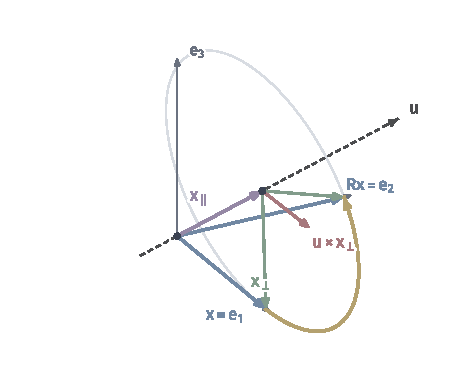
\includegraphics[width=80mm]{figures/04-spaces-measures-and-geometry/04-manifolds/matplotlib/lie-rodrigues-decomposition/figure.pdf}
  \caption{Rodrigues公式的分解。旋转轴$\bm u=(1,1,1)^\top/\sqrt3$，转角$2\pi/3$，$\bm x=\bm e_1$。紫色是沿轴分量$\bm x_\parallel$，保持不动；绿色是垂直分量$\bm x_\perp$，在灰色圆所在的平面内转动，转完后的绿色向量指向$\bm R\bm x$的末端；红色是$\bm u\times\bm x_\perp$的方向（长度按比例缩短）；黄色弧是端点走过的路径，终点是$\bm R\bm x=\bm e_2$。}
  \label{fig:lie-rodrigues-decomposition}
\end{BookInlineFigure}

\paragraph{每个旋转都有轴与角}
反过来，每个三维旋转都能写成式~\eqref{eq:lie-rodrigues}的形式，从而$\exp:\mathfrak{so}(3)\to\mathrm{SO}(3)$是满射。要证明这一点，先找出旋转的转轴，它是特征值$1$的特征向量，再看垂直于轴的平面。

\begin{theorem}[轴角表示]
\label{thm:lie-axis-angle}
对每个$\bm R\in\mathrm{SO}(3)$，存在单位向量$\bm u$与$\theta\in[0,\pi]$，使$\bm R=\exp(\theta[\bm u]_\times)$。并且
\begin{equation}
 \operatorname{tr}\bm R=1+2\cos\theta,\qquad \bm R-\bm R^\top=2\sin\theta\,[\bm u]_\times.
 \label{eq:lie-axis-angle-recovery}
\end{equation}
\end{theorem}

\begin{proof}
先找转轴。由$\bm R^\top\bm R=\bm I$与$\det\bm R=1$，得到
\[
\det(\bm R-\bm I)=\det\bigl(\bm R(\bm I-\bm R^\top)\bigr)
=\det(\bm I-\bm R^\top)=\det(\bm I-\bm R).
\]
三阶矩阵取负号使行列式变号，$\det(\bm I-\bm R)=-\det(\bm R-\bm I)$，于是$\det(\bm R-\bm I)=0$，存在单位向量$\bm u$使$\bm R\bm u=\bm u$。

再看与轴正交的平面。若$\bm x^\top\bm u=0$，则
\[
(\bm R\bm x)^\top\bm u=(\bm R\bm x)^\top(\bm R\bm u)=\bm x^\top\bm u=0,
\]
所以平面$\bm u^\perp$被$\bm R$映到自身。

取$\bm u^\perp$中的单位向量$\bm v$，令$\bm w=\bm u\times\bm v$，则$(\bm v,\bm w,\bm u)$是右手标准正交基。在这组基下$\bm R$的矩阵是分块对角的，左上二阶块正交，且行列式等于$\det\bm R=1$。由第~\ref{sec:lie-group-subgroup}节对$\mathrm{SO}(2)$的刻画，它等于某个$\bm R(\theta)$，$\theta\in[0,2\pi)$，即$\bm R\bm v=\cos\theta\,\bm v+\sin\theta\,\bm w$。

若$\theta\in(\pi,2\pi)$，把$\bm u$换成$-\bm u$、$\theta$换成$2\pi-\theta$，于是可取$\theta\in[0,\pi]$。这与定理~\ref{thm:lie-rodrigues}描述的作用在一组基上一致，所以二者相等。

最后，对式~\eqref{eq:lie-rodrigues}取迹。反对称矩阵的迹为零，并由式~\eqref{eq:lie-hat-square}，
\[
\operatorname{tr}[\bm u]_\times^2=\operatorname{tr}(\bm u\bm u^\top)-3=-2,
\]
于是
\[
\operatorname{tr}\bm R=3-2(1-\cos\theta)=1+2\cos\theta.
\]
减去转置时对称部分抵消，反对称部分加倍，得到第二式。
\end{proof}

这给出\term{轴角表示}（axis-angle representation），常把它合成一个向量$\bm\omega=\theta\bm u$，称为旋转向量。用式~\eqref{eq:lie-axis-angle-recovery}反算上面的循环轮换矩阵。它的迹为$0$，所以$\cos\theta=-\frac12$，$\theta=2\pi/3$。反对称部分给出
\[
\bm R-\bm R^\top=\begin{bmatrix}0&-1&1\\1&0&-1\\-1&1&0\end{bmatrix}
=2\sin\theta\,[\bm u]_\times,
\]
对照式~\eqref{eq:lie-hat-map}读出$\bm u\propto(1,1,1)^\top$，再由$2\sin\theta=\sqrt3$得到$\bm u=(1,1,1)^\top/\sqrt3$，回到了原来的轴和角。

\paragraph{冗余与特殊角度}
轴角表示有三类冗余。$(\bm u,\theta)$与$(-\bm u,-\theta)$给出同一旋转，$\theta$与$\theta+2\pi$也给出同一旋转，所以把$\theta$限制在$[0,\pi]$。在这个范围内，$0<\theta<\pi$时$\sin\theta>0$，式~\eqref{eq:lie-axis-angle-recovery}唯一地恢复$\theta$与$\bm u$。

剩下两个角度需要单独说明。$\theta=0$时$\bm R=\bm I$，任何轴都可以。$\theta=\pi$时$\bm R-\bm R^\top=\bm0$，轴$\bm u$与$-\bm u$给出同一旋转：绕一个轴转半圈，与绕相反的轴转半圈结果相同。

用旋转向量描述，映射$\bm\omega\mapsto\exp([\bm\omega]_\times)$把闭球$\{\lVert\bm\omega\rVert_2\leq\pi\}$映满$\mathrm{SO}(3)$；在开球$\lVert\bm\omega\rVert_2<\pi$内是单射，边界球面上互为相反数的两点给出同一个旋转。所以$\mathrm{SO}(3)$可以想象成一个实心球，球面上相对的点被粘合。

图~\ref{fig:lie-so3-ball}用这个模型画出绕$\bm e_3$的旋转：$\theta$从$0$增大到$\pi$时，$\bm\omega$沿半径走到$\pi\bm e_3$；继续增大，它从球面相对的一点$-\pi\bm e_3$重新进入，回到中心。这条路径在$\mathrm{SO}(3)$中是连续的闭合路径，并没有跳跃。

\begin{BookInlineFigure}
  \centering
  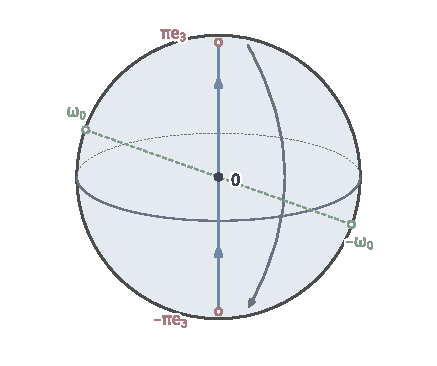
\includegraphics[width=74mm]{figures/04-spaces-measures-and-geometry/04-manifolds/matplotlib/lie-so3-ball/figure.pdf}
  \caption{$\mathrm{SO}(3)$的实心球模型。每个旋转向量$\bm\omega$的长度是转角，方向是转轴，闭球半径为$\pi$。边界上相对的两点（红圈$\pm\pi\bm e_3$，绿圈$\pm\bm\omega_0$）表示同一个旋转。蓝线是绕$\bm e_3$转一周的路径，走到$\pi\bm e_3$后，灰箭头表示它在$-\pi\bm e_3$处接着走，整条路径在$\mathrm{SO}(3)$中连续。}
  \label{fig:lie-so3-ball}
\end{BookInlineFigure}

在开球内，逆映射由式~\eqref{eq:lie-axis-angle-recovery}给出：
\[
\theta=\arccos\frac{\operatorname{tr}\bm R-1}{2},\qquad
[\bm\omega]_\times=\frac{\theta}{2\sin\theta}(\bm R-\bm R^\top),
\]
其中$\theta=0$处按极限$\theta/\sin\theta\to1$理解。所以旋转向量是$\mathrm{SO}(3)$去掉全部半圈旋转之后的局部坐标，与定理~\ref{thm:lie-so3-no-global-chart}一致：它不能延伸成全局坐标。

\paragraph{局部更新}
在一个已知旋转$\bm R$附近，常用$\bm R\exp([\bm\delta]_\times)$表示扰动后的旋转，其中$\bm\delta\in\mathbb R^3$很小。这是把单位元附近的指数坐标左平移到$\bm R$附近，参数$\bm\delta$在$\lVert\bm\delta\rVert_2<\pi$内与旋转一一对应。

一阶近似$\bm R+\bm R[\bm\delta]_\times$只是切空间中的一步，一般已不是正交矩阵；用指数代替它，结果严格留在$\mathrm{SO}(3)$中，这正是图~\ref{fig:lie-exp-limit}中折线与圆弧的区别。右乘$\exp([\bm\delta]_\times)$在物体自身的坐标系中扰动，左乘$\exp([\bm\delta]_\times)\bm R$则在固定的外部坐标系中扰动，二者一般不同，使用时须说明。

\paragraph{Euler角与万向节锁}
另一种常见的三参数记录是依次绕坐标轴旋转。记$\bm R_x,\bm R_y,\bm R_z$为绕三个坐标轴的旋转，取
\begin{equation}
 \bm R(\alpha,\beta,\gamma)=\bm R_z(\alpha)\bm R_y(\beta)\bm R_x(\gamma),
 \label{eq:lie-euler-angles}
\end{equation}
三个角称为一组\term{Euler角}（Euler angles）。它便于解释，却在特殊角度失去局部坐标的作用，原因在于三个参数对应的瞬时转轴可能共线。

把式~\eqref{eq:lie-euler-angles}分别对三个角求导，再右乘$\bm R^\top$，得到每个参数产生的角速度方向。用$\bm R_z(\alpha)$与$\bm R_y(\beta)$共轭后，三个方向是
\[
\bm a_\alpha=\bm e_3,\qquad
\bm a_\beta=\bm R_z(\alpha)\bm e_2,\qquad
\bm a_\gamma=\bm R_z(\alpha)\bm R_y(\beta)\bm e_1 .
\]
以$\bm a_\gamma$为例，把$\bm R_x$的导数写成$\bm R_x[\bm e_1]_\times$（绕$\bm e_1$转动的方向），再把两侧的转动并进叉积，得到
\[
\partial_\gamma\bm R\,\bm R^\top
=\bm R_z\bm R_y[\bm e_1]_\times\bm R_y^\top\bm R_z^\top
=[\bm R_z\bm R_y\bm e_1]_\times .
\]

这三个方向的线性无关性决定了参数化是否满秩。由
\[
\bm R_y(\beta)\bm e_1=(\cos\beta,0,-\sin\beta)^\top,
\]
并把三个向量都乘以$\bm R_z(\alpha)^\top$（不改变行列式），得到
\[
\det[\bm a_\alpha,\bm a_\beta,\bm a_\gamma]
=\det\begin{bmatrix}0&0&\cos\beta\\0&1&0\\1&0&-\sin\beta\end{bmatrix}
=-\cos\beta .
\]
当$\beta=\pm\pi/2$时行列式为零，参数到旋转的微分秩降为$2$。

\begin{BookInlineFigure}
  \centering
  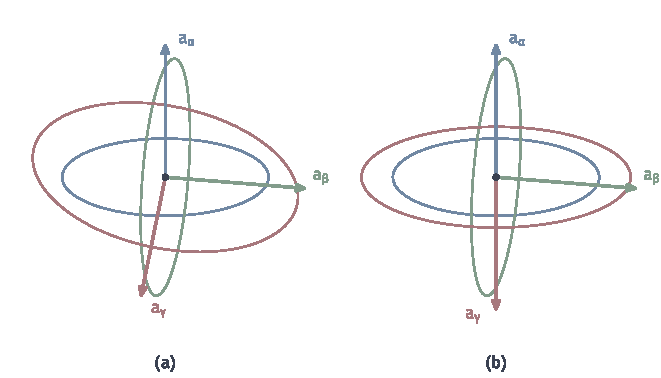
\includegraphics[width=112mm]{figures/04-spaces-measures-and-geometry/04-manifolds/matplotlib/lie-gimbal-lock/figure.pdf}
  \caption{Euler角的三个瞬时转轴。蓝、绿、红箭头分别是$\alpha,\beta,\gamma$对应的转轴$\bm a_\alpha,\bm a_\beta,\bm a_\gamma$，同色圆环垂直于该轴（这里$\alpha=20^\circ$）。(a)$\beta=35^\circ$，三根轴线性无关，任何方向的小转动都能实现。(b)$\beta=90^\circ$，$\bm a_\gamma=-\bm e_3$与$\bm a_\alpha$共线，两个圆环重合在同一平面内，只剩两个独立的转动方向。}
  \label{fig:lie-gimbal-lock}
\end{BookInlineFigure}

直接代入也能看到这一点。由$\bm R_y(\pi/2)\bm e_1=-\bm e_3$，绕$\bm e_1$的旋转经$\bm R_y(\pi/2)$共轭后变为绕$-\bm e_3$的旋转，即
\[
\bm R_y(\tfrac\pi2)\bm R_x(\gamma)=\bm R_z(-\gamma)\bm R_y(\tfrac\pi2).
\]
于是
\[
\bm R(\alpha,\tfrac\pi2,\gamma)=\bm R_z(\alpha-\gamma)\bm R_y(\tfrac\pi2).
\]
结果只依赖$\alpha-\gamma$：同时把$\alpha,\gamma$加上同一个数，旋转不变。这称为\term{万向节锁}（gimbal lock），图~\ref{fig:lie-gimbal-lock}(b)中蓝、红两根轴共线正是它的几何原因。

万向节锁是坐标的奇异，不是旋转本身的退化。$\bm R(\alpha,\pi/2,\gamma)$仍是合法的旋转，$\mathrm{SO}(3)$在它附近仍是三维流形；只是这一组角在该处不能作为坐标，附近的小转动也可能要求角度大幅跳动。换一种轴的次序或改用旋转向量，就能在这里重新得到正常的局部坐标。

\subsection{单位四元数}
\label{sec:lie-unit-quaternions}

旋转矩阵用九个数，轴角在半圈处与恒等处需要特别处理。单位四元数用四个数和一个单位长度约束记录旋转，复合只需一次乘法，并且在每一点附近都给出正常的局部坐标，代价是每个旋转恰有两个记录。

\paragraph{四元数及其运算}
把\term{四元数}（quaternion）写成标量部与三维向量部组成的对$q=(s,\bm u)$，其中$s\in\mathbb R$、$\bm u\in\mathbb R^3$。加法与数乘按$\mathbb R^4$进行，乘法规定为
\begin{equation}
 (s,\bm u)(t,\bm v)=(st-\bm u^\top\bm v,\ s\bm v+t\bm u+\bm u\times\bm v).
 \label{eq:lie-quaternion-product}
\end{equation}
类比复数：标量部相当于实部，向量部相当于“虚部”，只是虚部有三个方向，它们之间的乘法由叉积描述。

因为含有叉积，乘法一般不交换：$(0,\bm e_1)(0,\bm e_2)=(0,\bm e_3)$，而$(0,\bm e_2)(0,\bm e_1)=(0,-\bm e_3)$。$(1,\bm0)$是乘法单位元。乘法满足结合律，把三重乘积按式~\eqref{eq:lie-quaternion-product}展开，用二重叉积公式整理即可验证，这里略去这段机械的展开。

共轭定义为$q^*=(s,-\bm u)$，范数定义为$\lvert q\rvert=\sqrt{s^2+\lVert\bm u\rVert_2^2}$，即$\mathbb R^4$中的欧氏长度。由式~\eqref{eq:lie-quaternion-product}，
\[
qq^*=\bigl(s^2+\bm u^\top\bm u,\ -s\bm u+s\bm u-\bm u\times\bm u\bigr)
=(\lvert q\rvert^2,\bm0),
\]
同理$q^*q=(\lvert q\rvert^2,\bm0)$。直接展开还可验证$(pq)^*=q^*p^*$。

下面的引理说明范数与乘法相容，这是四元数能表示旋转的基础。

\begin{lemma}[范数的乘法性]
\label{lem:lie-quaternion-norm}
对四元数$p,q$，$\lvert pq\rvert=\lvert p\rvert\,\lvert q\rvert$。因此$\lvert q\rvert=1$的\term{单位四元数}（unit quaternion）在乘法下构成群，$q^{-1}=q^*$；作为集合，它就是$\mathbb R^4$中的单位球面$S^3$。
\end{lemma}

\begin{proof}
设$p=(s,\bm u)$、$q=(t,\bm v)$。向量部$s\bm v+t\bm u+\bm u\times\bm v$中，$\bm u\times\bm v$与$\bm u,\bm v$都正交，所以
\[
\lvert pq\rvert^2=(st-\bm u^\top\bm v)^2+\lVert s\bm v+t\bm u\rVert_2^2+\lVert\bm u\times\bm v\rVert_2^2.
\]
展开平方后，交叉项$-2st\,\bm u^\top\bm v$与$+2st\,\bm u^\top\bm v$相消，剩下
\[
s^2t^2+s^2\lVert\bm v\rVert_2^2+t^2\lVert\bm u\rVert_2^2+(\bm u^\top\bm v)^2+\lVert\bm u\times\bm v\rVert_2^2.
\]
由Lagrange恒等式
\[
(\bm u^\top\bm v)^2+\lVert\bm u\times\bm v\rVert_2^2=\lVert\bm u\rVert_2^2\lVert\bm v\rVert_2^2,
\]
上式等于
\[
(s^2+\lVert\bm u\rVert_2^2)(t^2+\lVert\bm v\rVert_2^2).
\]
于是单位四元数的乘积仍是单位四元数，$qq^*=(1,\bm0)$给出逆元，结合律继承自全体四元数。
\end{proof}

\paragraph{用共轭作用表示旋转}
把向量$\bm x$嵌入为向量部，即纯四元数$(0,\bm x)$。对单位四元数$q=(s,\bm u)$，分两步计算$q(0,\bm x)q^*$。先由式~\eqref{eq:lie-quaternion-product}左乘，得到
\[
q(0,\bm x)=(-\bm u^\top\bm x,\ s\bm x+\bm u\times\bm x).
\]

再右乘$q^*=(s,-\bm u)$。标量部是
\[
(-\bm u^\top\bm x)s+(s\bm x+\bm u\times\bm x)^\top\bm u=0,
\]
这是因为$\bm u\times\bm x$与$\bm u$正交。向量部用二重叉积公式
\[
(\bm u\times\bm x)\times\bm u=\lVert\bm u\rVert_2^2\bm x-(\bm u^\top\bm x)\bm u
\]
整理，得到
\begin{equation}
 \begin{gathered}
 q(0,\bm x)q^*=(0,\bm R(q)\bm x),\\
 \bm R(q)\bm x=(s^2-\lVert\bm u\rVert_2^2)\bm x+2\bm u(\bm u^\top\bm x)+2s\,\bm u\times\bm x.
 \end{gathered}
 \label{eq:lie-quaternion-rotation}
\end{equation}

取$q=(\cos\frac\theta2,\ \sin\frac\theta2\,\bm a)$，其中$\lVert\bm a\rVert_2=1$。由半角公式，
\[
s^2-\lVert\bm u\rVert_2^2=\cos\theta,\qquad
2\bm u\bm u^\top=(1-\cos\theta)\bm a\bm a^\top,\qquad
2s\bm u=\sin\theta\,\bm a.
\]
代入式~\eqref{eq:lie-quaternion-rotation}，再用式~\eqref{eq:lie-hat-square}，得到
\[
\begin{aligned}
\bm R(q)
&=\cos\theta\,\bm I+(1-\cos\theta)\bm a\bm a^\top+\sin\theta\,[\bm a]_\times\\
&=\bm I+\sin\theta\,[\bm a]_\times+(1-\cos\theta)[\bm a]_\times^2 .
\end{aligned}
\]
这正是Rodrigues公式~\eqref{eq:lie-rodrigues}：$q$表示绕$\bm a$转角$\theta$。半角来自$q$在两侧各乘一次，不是把物理转角减半。

\paragraph{复合与双覆盖}
手算两个旋转的复合。设$q_1=(\frac{\sqrt2}2,\ \frac{\sqrt2}2\bm e_3)$表示绕$\bm e_3$转$90^\circ$，$q_2=(\frac{\sqrt2}2,\ \frac{\sqrt2}2\bm e_1)$表示绕$\bm e_1$转$90^\circ$，先做$q_1$、再做$q_2$。由式~\eqref{eq:lie-quaternion-product}，
\[
q_2q_1=\Bigl(\tfrac12,\ \tfrac12\bm e_3+\tfrac12\bm e_1+\tfrac12\bm e_1\times\bm e_3\Bigr)
=\Bigl(\tfrac12,\ \tfrac12(1,-1,1)^\top\Bigr).
\]

读出半角：$\cos\frac\theta2=\frac12$，所以$\theta=2\pi/3$，转轴是$(1,-1,1)^\top/\sqrt3$。用式~\eqref{eq:lie-quaternion-rotation}计算$\bm e_1$的像，三项分别是$-\frac12\bm e_1$、$\frac12(1,-1,1)^\top$、$\frac12(0,1,1)^\top$，相加得到$\bm e_3$。

直接用矩阵核对，
\[
\bm R_x(\tfrac\pi2)\bm R_z(\tfrac\pi2)\bm e_1=\bm R_x(\tfrac\pi2)\bm e_2=\bm e_3 ,
\]
结果一致。复合用四元数只需一次乘法，读出轴和角也只需看四个数。

这个计算说明的是一般事实。由结合律与$(q_2q_1)^*=q_1^*q_2^*$，
\[
(q_2q_1)(0,\bm x)(q_2q_1)^*=q_2\bigl(q_1(0,\bm x)q_1^*\bigr)q_2^* ,
\]
即$\bm R(q_2q_1)=\bm R(q_2)\bm R(q_1)$。所以$q\mapsto\bm R(q)$是从单位四元数群到$\mathrm{SO}(3)$的群同态。由定理~\ref{thm:lie-axis-angle}，每个旋转都有轴与角，从而有形如上式的四元数，这个同态是满射。它的核由下面的定理确定。

\begin{theorem}[单位四元数的双覆盖]
\label{thm:lie-double-cover}
对单位四元数$q_1,q_2$，$\bm R(q_1)=\bm R(q_2)$当且仅当$q_2=\pm q_1$。
\end{theorem}

\begin{proof}
由定理~\ref{thm:lie-kernel-injective}，只需证明核为$\{(1,\bm0),(-1,\bm0)\}$。设$q=(s,\bm u)$是单位四元数，$\bm R(q)=\bm I$。

若$\bm u\neq\bm0$，取与$\bm u$正交的非零向量$\bm x$。由式~\eqref{eq:lie-quaternion-rotation}与$s^2+\lVert\bm u\rVert_2^2=1$，$\bm x=\bm R(q)\bm x$成为
\[
\bm x=(1-2\lVert\bm u\rVert_2^2)\bm x+2s\,\bm u\times\bm x,
\]
移项得到
\[
-2\lVert\bm u\rVert_2^2\bm x+2s\,\bm u\times\bm x=\bm0 .
\]
两项分别与$\bm x$平行、与$\bm x$正交，必须各为零，第一项非零，矛盾。

所以$\bm u=\bm0$，由单位长度得$s=\pm1$。反过来，$\pm(1,\bm0)$代入式~\eqref{eq:lie-quaternion-rotation}给出$\bm I$。
\end{proof}

这称为单位四元数对$\mathrm{SO}(3)$的\term{双覆盖}（double cover）：每个旋转恰有两个单位四元数，二者互为相反数。上面的$q_1$与$-q_1=(-\frac{\sqrt2}2,-\frac{\sqrt2}2\bm e_3)$表示同一个旋转，后者对应转角$\pi/2+2\pi$的半角。图~\ref{fig:lie-double-cover}把$S^3$限制到一条大圆上画出这个现象。

\begin{BookInlineFigure}
  \centering
  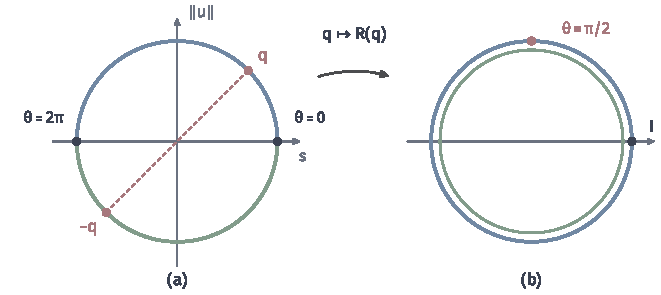
\includegraphics[width=112mm]{figures/04-spaces-measures-and-geometry/04-manifolds/matplotlib/lie-double-cover/figure.pdf}
  \caption{半角与双覆盖。固定转轴$\bm a$，单位四元数$(\cos\frac\theta2,\sin\frac\theta2\,\bm a)$在$S^3$中走出一条大圆。(a)这条大圆，横轴为标量部，纵轴为沿$\bm a$的向量部。$\theta$从$0$到$2\pi$时走过蓝色半圆，从$2\pi$到$4\pi$时走过绿色半圆，$q$与$-q$（红点）相对。(b)绕$\bm a$的旋转组成的圆，$\theta$走一周即回到$\bm I$，蓝、绿两个半圆分别映满整个圆，$q$与$-q$映到同一点。}
  \label{fig:lie-double-cover}
\end{BookInlineFigure}

双覆盖与坐标奇异是两回事。$q\mapsto\bm R(q)$在每一点都是局部微分同胚。在$q=(1,\bm0)$附近，
\[
\bm R(q)=\bm I+2[\bm u]_\times+O(\lVert\bm u\rVert_2^2),
\]
微分$\bm u\mapsto2[\bm u]_\times$是从切空间$T_{(1,\bm0)}S^3=\{(0,\bm u)\}$到$\mathfrak{so}(3)$的线性同构；在其他点用群乘法平移即得。

所以单位四元数在任何朝向附近都给出正常的局部坐标，不会出现Euler角那样的秩下降。$q$与$-q$之差也不是额外的物理自由度：$S^3$与$\mathrm{SO}(3)$都是三维，符号只是整体上的二选一。

\paragraph{计算中的注意事项}
按式~\eqref{eq:lie-quaternion-product}，两个四元数相乘需要$16$次实数乘法，两个三阶矩阵相乘需要$27$次。数值计算中多次相乘会使$\lvert q\rvert$逐渐偏离$1$；若$\lvert q\rvert\neq1$，$q(0,\bm x)q^*$会额外把$\bm x$放大$\lvert q\rvert^2$倍，不再是旋转，所以需要定期把$q$除以$\lvert q\rvert$。

比较两个四元数是否接近时，还要考虑符号：$q$与$-q$在$\mathbb R^4$中相距$2$，表示的却是同一个旋转。表~\ref{tab:lie-rotation-representations}汇总了本节比较的各种表示。

\begin{BookInlineTable}
  \centering
  \caption{三维旋转的几种表示}
  \label{tab:lie-rotation-representations}
  \begin{tabular}{lll}
    \toprule
    表示 & 参数与约束 & 冗余或奇异 \\
    \midrule
    旋转矩阵 & $9$个数，$6$个约束 & 无冗余，运算需保持约束 \\
    轴角 & $3$个数，$\lVert\bm\omega\rVert_2\leq\pi$ & 半圈处$\pm\bm\omega$相同 \\
    Euler角 & $3$个数 & $\beta=\pm\pi/2$处秩降为$2$ \\
    单位四元数 & $4$个数，$1$个约束 & $q$与$-q$相同，无奇异 \\
    \bottomrule
  \end{tabular}
\end{BookInlineTable}

\section{刚体位姿}
\label{sec:lie-rigid-poses}

一个刚体在空间中的状态由两部分决定：它朝向哪里，以及它的参考点在哪里。前者是上一节的旋转，后者是一个平移。可以证明，保持任意两点距离与空间定向的变换恰好是先旋转、再平移的复合（这里不给出证明）；这样的变换称为\term{刚体变换}（rigid transformation），它描述的状态称为\term{位姿}（pose）。本节建立刚体变换的复合与求逆，说明它在点与方向上的不同作用，最后用它表达坐标系之间的换算。

\paragraph{齐次矩阵}
刚体变换把$\bm x$变成$\bm R\bm x+\bm t$，其中$\bm R\in\mathrm{SO}(3)$、$\bm t\in\mathbb R^3$。它不是线性映射，因为原点被移到$\bm t$。在每个点后面补一个坐标$1$，就能把它写成一次矩阵乘法：
\begin{equation}
 \begin{bmatrix}\bm R\bm x+\bm t\\1\end{bmatrix}=\bm T\begin{bmatrix}\bm x\\1\end{bmatrix},\qquad
 \bm T=\begin{bmatrix}\bm R&\bm t\\\bm0^\top&1\end{bmatrix}.
 \label{eq:lie-homogeneous-pose}
\end{equation}
这样的$4\times4$矩阵全体记为$\mathrm{SE}(3)$，称为\term{三维刚体运动群}（three-dimensional rigid-motion group）。

\paragraph{复合与求逆}
按分块乘法，先作用$\bm T_1$、再作用$\bm T_2$得到
\begin{equation}
 \bm T_2\bm T_1=\begin{bmatrix}\bm R_2\bm R_1&\bm R_2\bm t_1+\bm t_2\\\bm0^\top&1\end{bmatrix},\qquad
 \bm T^{-1}=\begin{bmatrix}\bm R^\top&-\bm R^\top\bm t\\\bm0^\top&1\end{bmatrix}.
 \label{eq:lie-pose-composition}
\end{equation}
乘积仍是同样形状的矩阵，逆矩阵也是，单位元是$\bm I_4$，所以$\mathrm{SE}(3)$是$\mathrm{GL}(4,\mathbb R)$的子群。求逆的公式可以直接解出：由$\bm y=\bm R\bm x+\bm t$得$\bm x=\bm R^\top(\bm y-\bm t)=\bm R^\top\bm y-\bm R^\top\bm t$。

复合的平移部分是$\bm R_2\bm t_1+\bm t_2$，而不是$\bm t_1+\bm t_2$：第一次的平移要随第二次的旋转一起转动。例如两次都绕$\bm e_3$转$\pi/2$，平移分别为$\bm t_1=(1,0,0)^\top$与$\bm t_2=(0,1,0)^\top$。复合的旋转是绕$\bm e_3$转$\pi$，平移是$\bm R_2\bm t_1+\bm t_2=(0,1,0)^\top+(0,1,0)^\top=(0,2,0)^\top$。按另一次序复合，平移变成$\bm R_1\bm t_2+\bm t_1=(-1,0,0)^\top+(1,0,0)^\top=\bm0$，结果不同。

\paragraph{作为Lie群}
$\mathrm{SE}(3)$在$\mathrm{GL}(4,\mathbb R)$中由“左上块在$\mathrm{SO}(3)$中、末行为$(0,0,0,1)$”这些闭条件给出，是闭子群，因而是矩阵Lie群。$(\bm R,\bm t)\mapsto\bm T$是从$\mathrm{SO}(3)\times\mathbb R^3$到$\mathrm{SE}(3)$的微分同胚，所以$\mathrm{SE}(3)$是六维流形：三个旋转自由度加三个平移自由度。但作为群，它不是$\mathrm{SO}(3)$与$\mathbb R^3$的直积：直积的运算会给出$(\bm R_2\bm R_1,\bm t_1+\bm t_2)$，而式~\eqref{eq:lie-pose-composition}中旋转会作用到前一次的平移上。

对经过$\bm I_4$的曲线求导，末行恒为零、左上块的导数在$\mathfrak{so}(3)$中，所以Lie代数是
\[
\mathfrak{se}(3)=\left\{\begin{bmatrix}[\bm\omega]_\times&\bm v\\\bm0^\top&0\end{bmatrix}:\bm\omega,\bm v\in\mathbb R^3\right\}.
\]
用归纳法可得，对$k\geq1$，该矩阵的$k$次幂是$\begin{bmatrix}[\bm\omega]_\times^k&[\bm\omega]_\times^{k-1}\bm v\\\bm0^\top&0\end{bmatrix}$，于是
\[
\exp\begin{bmatrix}[\bm\omega]_\times&\bm v\\\bm0^\top&0\end{bmatrix}
=\begin{bmatrix}\exp([\bm\omega]_\times)&\bm V\bm v\\\bm0^\top&1\end{bmatrix},\qquad
\bm V=\sum_{k\geq0}\frac{[\bm\omega]_\times^k}{(k+1)!}.
\]
$\bm\omega=\bm0$时$\bm V=\bm I$，指数就是平移$\bm v$；$\bm\omega\neq\bm0$时，平移部分是$\bm V\bm v$而不是$\bm v$，单参数子群一般绕某条轴转动、同时沿该轴推进（推进量可以为零），是一种螺旋运动。所以$\mathrm{SE}(3)$上的指数坐标不等于“旋转向量加平移向量”这种分开的记录，使用时须说明采用哪一种参数化。

\paragraph{点与方向}
位姿对点和方向的作用不同。点有位置，平移会移动它；方向只有朝向，例如速度、表面法向或两点之差，平移不应改变它。设$\bm x,\bm y$是两个点，它们的差在变换后为$(\bm R\bm x+\bm t)-(\bm R\bm y+\bm t)=\bm R(\bm x-\bm y)$，平移抵消了。在齐次写法中，把点记为$(\bm x,1)$，把方向记为$(\bm d,0)$，则
\[
\bm T\begin{bmatrix}\bm d\\0\end{bmatrix}=\begin{bmatrix}\bm R\bm d\\0\end{bmatrix},
\]
末坐标$0$恰好让平移列不起作用，两个点之差的末坐标也自然是$1-1=0$。

点与方向的区分在计算中容易出错。把方向向量当成点，用$\bm R\bm d+\bm t$变换，会给方向加上一个与位姿有关的偏移；把点当成方向，则会丢掉平移。若变换是一般的可逆线性映射$\bm A$而不是旋转，法向量要按$\bm A^{-\top}$变换才能保持与切向量的正交；对旋转，$\bm R^{-\top}=\bm R$，法向与其他方向按同一规则变换。

\paragraph{坐标系变换}
同一个点在不同坐标系中有不同的坐标，刚体变换也负责这种换算。设坐标系$B$的原点在坐标系$A$中的坐标为$\bm t_{AB}$，$B$的三个坐标轴在$A$中的方向依次是$\bm R_{AB}$的三列。若一点在$B$中的坐标为$\bm x_B$，它在$A$中的位置是$B$的原点加上沿$B$各轴的位移，即
\[
\bm x_A=\bm R_{AB}\bm x_B+\bm t_{AB},\qquad
\bm T_{AB}=\begin{bmatrix}\bm R_{AB}&\bm t_{AB}\\\bm0^\top&1\end{bmatrix}.
\]
这里$\bm T_{AB}$读作“从$B$的坐标到$A$的坐标”。由此得到两条规则：经过中间坐标系$B$换算，$\bm T_{AC}=\bm T_{AB}\bm T_{BC}$，相邻下标相同才能相乘；反向换算是求逆，$\bm T_{BA}=\bm T_{AB}^{-1}$。

同一个矩阵$\bm T_{AB}$有两种读法：它可以看作把点从一个位置移到另一个位置的主动变换，也可以看作同一个点在两个坐标系之间的坐标换算。两种读法使用同一套矩阵运算，但描述的对象不同；混淆二者，最常见的后果是该用$\bm T$的地方用了$\bm T^{-1}$，或者乘积次序颠倒。

给定一组点在两个坐标系中的对应坐标，要反求$\bm R_{AB}$与$\bm t_{AB}$，这就是由点对应估计刚体变换的问题。它需要拟合目标、正交约束下的求解与可辨识性分析，在第~\ref{chap:spatial-map-estimation}章研究。

\section{商流形}
\label{sec:lie-quotients}

前面几节反复遇到“多种记录代表同一对象”：$q$与$-q$表示同一个旋转；图~\ref{fig:lie-sphere-cosets}中一整圈旋转把$\bm e_3$送到同一个点；一个观测只确定方向时，$(2,1)^\top$与$(4,2)^\top$应视为同一对象；同一个子空间可以用许多组基张成。这些冗余都来自一个群作用：它作用在记录上，而不改变所表示的对象。把同一轨道中的记录合并，就得到真正要研究的对象集合。

第~\ref{chap:topological-spaces}章为等价关系的商集合规定了商拓扑：设$q:M\to M/G$把每个点送到所在的轨道，商中的子集$U$为开集，当且仅当$q^{-1}(U)$在$M$中为开集。本节要进一步回答：什么时候这个商还能带上光滑结构，使后面几章的切空间、微分与度量都能使用。任意群作用的商一般做不到这一点。

\subsection{光滑商的条件}
\label{sec:lie-smooth-quotient-conditions}

先看两个商不是流形的例子，从中读出群作用需要满足的条件，再陈述这些条件下的商流形定理，并用闭子群构造最常用的一类商。

\paragraph{两类失败}
第一类失败来自稳定子不一致。第~\ref{sec:lie-orbits-stabilizers}节中，$\mathrm{SO}(2)$作用于$\mathbb R^2$的商是$[0,\infty)$。非零点的轨道是圆，稳定子平凡；原点的轨道是一个点，稳定子是整个群。商在$0$处有一个端点，那里的任何邻域都不同胚于开区间，所以商不是无边界的一维流形，见图~\ref{fig:lie-quotient-failures}(a)(b)。不能只因为“去掉了一个旋转自由度”就宣布商是$2-1=1$维流形。

第二类失败来自轨道挤在一起。取无理数$\alpha$，让整数加法群$\mathbb Z$按$k\cdot\bm x=\bm R(2\pi k\alpha)\bm x$作用在单位圆上。$k\neq0$时$k\alpha$不是整数，没有点被固定，稳定子都是平凡的。但每条轨道都在圆上稠密。

下面证明这一点。把圆分成$N$段长为$2\pi/N$的弧，同一条轨道上$k=0,1,\ldots,N$这$N+1$个点必有两个落在同一段，设为$k_1<k_2$。令$k=k_2-k_1$，则转角$2\pi k\alpha$模$2\pi$后绝对值小于$2\pi/N$，且不为零。反复施加这个小旋转，轨道上就出现间距小于$2\pi/N$的点，$N$可以任意大，所以轨道稠密。

\begin{BookInlineFigure}
  \centering
  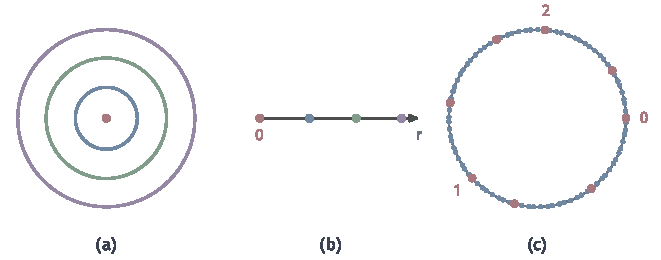
\includegraphics[width=112mm]{figures/04-spaces-measures-and-geometry/04-manifolds/matplotlib/lie-quotient-failures/figure.pdf}
  \caption{商不是流形的两种情形。(a)$\mathrm{SO}(2)$作用于平面的轨道：同心圆与中心的原点。(b)轨道空间$[0,\infty)$，用半径编号，同色的点对应同色的圆，原点（红）对应端点。(c)无理旋转的一条轨道，$\alpha=(\sqrt5-1)/2$，大红点依次是前$8$个点$k=0,\ldots,7$，小蓝点是$k=8,\ldots,89$，已经密布整个圆。}
  \label{fig:lie-quotient-failures}
\end{BookInlineFigure}

于是商空间的拓扑很差。设$U$是商中的非空开集，它的原像是圆上的非空开集，且由整条轨道组成。任何一条轨道都稠密，所以都与这个开集相交，从而整条轨道都在其中，$U$就是整个商。商的开集只有空集和全集，不同的点不能被开集分开，它不是Hausdorff空间，更不是流形。

\paragraph{自由与适当}
这两类失败分别对应下面两个条件。

\begin{definition}[自由作用与适当作用]
\label{def:lie-free-proper-action}
设Lie群$G$光滑地作用于流形$M$，即$G\times M\to M$是光滑映射。若每个点的稳定子都只含单位元，就称作用是\term{自由作用}（free action）。若映射$G\times M\to M\times M$，$(g,x)\mapsto(g\cdot x,x)$下每个紧集的原像都是紧集，就称作用是\term{适当作用}（proper action）。
\end{definition}

自由性排除了第一类失败：各点的稳定子相同，轨道的维数处处等于群的维数。适当性排除了第二类失败：它禁止群中“跑到无穷远”的元素把一个点又带回原处附近，从而使不同的轨道能被邻域分开。

紧Lie群的光滑作用总是适当的，有限群作为零维Lie群也是如此。上面的$\mathbb Z$作用不适当：取$\bm x$的一个邻域，无穷多个$k$把$\bm x$送回这个邻域，这些$k$组成无界的集合。下面的定理说明，这两个条件足以得到光滑的商。

\begin{theorem}[商流形定理]
\label{thm:lie-quotient-manifold}
设Lie群$G$在$m$维光滑流形$M$上的光滑作用既自由又适当，$G$的维数为$k$。则轨道空间$M/G$在商拓扑下是$m-k$维的拓扑流形，并且具有唯一的光滑结构，使商映射$q:M\to M/G$是光滑淹没。
\end{theorem}

定理的证明需要构造横截于轨道的局部切片，并用常秩定理验证转移映射光滑，篇幅较长，读者可查阅\scite{math-lee2013smooth}。证明的思路是：在每个点附近，取与轨道横截的一小片子流形，由自由与适当两个条件，每条附近的轨道与这片子流形恰好相交一次，这片子流形就充当商的坐标图。

所得的光滑结构称为\term{商流形}（quotient manifold）。由$q$是淹没，$M/G$上的映射$f$光滑，当且仅当$f\circ q$在$M$上光滑。第~\ref{sec:lie-invariant-equivariant}节中经由轨道分解的不变映射，正是用这种方式落到商上。

定理给的是充分条件，不是唯一可用的情形。对没有给定作用的一般等价关系，商可能根本不是流形；即使作用存在，也要逐项核对光滑、自由与适当，不能把任意等价关系的商都当作光滑流形。

\paragraph{齐性空间}
最常用的一类商来自闭子群。设$H$是Lie群$G$的闭子群，它按$h\cdot g=gh^{-1}$作用在$G$上，轨道恰是左陪集$gH$。这个作用自由，并且可以证明是适当的（闭性保证陪集不会挤在一起），所以$G/H$是$\dim G-\dim H$维的流形，称为\term{齐性空间}（homogeneous space）。它之所以“齐性”，是因为$G$按$g'\cdot(gH)=(g'g)H$传递地作用在$G/H$上，任何两点之间都有一个变换相连。

齐性空间常常就是某个熟悉的空间。若$G$光滑且传递地作用于流形$X$，$x_0\in X$的稳定子为$H$，由定理~\ref{thm:lie-orbit-stabilizer}，$gH\mapsto g\cdot x_0$是从$G/H$到$X$的双射，并且可以进一步证明它是微分同胚。以$\mathrm{SO}(3)$作用于$S^2$为例，$\bm e_3$的稳定子是绕第三轴的旋转，与$\mathrm{SO}(2)$同构，所以
\begin{equation}
 \mathrm{SO}(3)/\mathrm{SO}(2)\cong S^2,\qquad \bm R\,\mathrm{SO}(2)\mapsto\bm R\bm e_3.
 \label{eq:lie-so3-so2}
\end{equation}

维数核对：$3-1=2$。图~\ref{fig:lie-sphere-cosets}(b)画的正是这个商的一条纤维：$\bm R$的第三列决定了陪集，前两列在切平面内还可以任意转动，这一转动正是被商掉的自由度。

另一个例子回到四元数。有限群$\{(1,\bm0),(-1,\bm0)\}$按左乘作用在$S^3$上，没有不动点，作用自由且适当，商$S^3/\{\pm1\}$是三维流形。由定理~\ref{thm:lie-double-cover}，$q\mapsto\bm R(q)$在每条轨道$\{q,-q\}$上取同一个值，并且不同的轨道给出不同的旋转，于是它在商上给出$S^3/\{\pm1\}$到$\mathrm{SO}(3)$的双射；结合它是局部微分同胚，可知这个双射是微分同胚。

\subsection{射影空间}
\label{sec:lie-projective-space}

相机把空间中的一点投影到成像平面时，只能确定这一点所在的视线方向，不能确定它沿视线有多远。若把视线用一个非零向量记录，那么$\bm x$与$\lambda\bm x$（$\lambda\neq0$）记录的是同一条视线。忽略这种非零倍数，就得到射影空间。

\begin{definition}[实射影空间]
\label{def:lie-projective-space}
非零实数在乘法下构成群$\mathbb R^*=\mathbb R\setminus\{0\}$，它按$\lambda\cdot\bm x=\lambda\bm x$作用于$\mathbb R^{n+1}\setminus\{\bm0\}$。轨道空间
\begin{equation}
 \mathbb{RP}^n=(\mathbb R^{n+1}\setminus\{\bm0\})/\mathbb R^*
 \label{eq:lie-rpn}
\end{equation}
称为$n$维\term{实射影空间}（real projective space）。$\bm x$所在的轨道记为$[\bm x]=[x_1:\cdots:x_{n+1}]$，称为\term{齐次坐标}（homogeneous coordinates）。
\end{definition}

$\mathbb{RP}^n$的一个点就是$\mathbb R^{n+1}$中过原点的一条直线。零向量必须除去：它的所有倍数都是零，不表示任何方向。这个作用是自由的，因为$\lambda\bm x=\bm x$与$\bm x\neq\bm0$推出$\lambda=1$。

作用也是适当的。设$K$是$(\mathbb R^{n+1}\setminus\{\bm0\})^2$中的紧集，$K$的两个分量的范数都落在某个区间$[a,b]$内，$a>0$。若$(\lambda\bm x,\bm x)\in K$，则
\[
\lvert\lambda\rvert=\frac{\lVert\lambda\bm x\rVert_2}{\lVert\bm x\rVert_2}\in\Bigl[\frac ab,\frac ba\Bigr].
\]
所以原像中的$\lambda$在$\mathbb R^*$的紧子集内，$\bm x$在$K$的投影内，原像又是闭集，从而是紧集。由定理~\ref{thm:lie-quotient-manifold}，$\mathbb{RP}^n$是$n$维光滑流形，维数核对$(n+1)-1=n$。把代表元缩放到单位球面，只剩符号自由度，于是它也可以写成$S^n/\{\pm1\}$。

\paragraph{仿射图与无穷远点}
商流形的坐标可以直接写出来。在$x_j\neq0$的点上，每个类都唯一地有一个代表使第$j$个分量为$1$，于是令
\[
U_j=\{[\bm x]:x_j\neq0\},\qquad
\varphi_j([\bm x])=\Bigl(\frac{x_i}{x_j}\Bigr)_{i\neq j}\in\mathbb R^n .
\]
$\varphi_j$不依赖代表元，因为分子分母同乘$\lambda$。$U_j$的原像$\{x_j\neq0\}$是开集，所以$U_j$是开集。$\varphi_j\circ q$是有理函数，因而连续；逆映射把$\bm u$送到第$j$分量为$1$的向量再取类，也连续，所以$\varphi_j$是同胚。两张图的重叠处，坐标转换是分量之比，分母非零，因而光滑。这些图称为\term{仿射图}（affine chart），$n+1$张就覆盖了$\mathbb{RP}^n$。

相对于一张选定的仿射图$U_{n+1}$，不在其中的点$\{x_{n+1}=0\}$称为\term{无穷远点}（point at infinity）。它们不是向坐标中加入数值$\infty$，而是这张图未覆盖、在其他图中可以正常记录的点。

看$\mathbb{RP}^1$的例子。末分量图中，每条不水平的直线与直线$x_2=1$恰好相交一次，交点的第一坐标$x_1/x_2$就是这条直线的坐标，见图~\ref{fig:lie-projective}(a)。例如$[2:4]=[1:2]$的坐标是$\frac12$。水平线$[1:0]$与$x_2=1$不相交，它不在这张图中，但在首分量图中坐标为$0$。所以$\mathbb{RP}^1$是一条直线加上一个无穷远点，拓扑上是一个圆。

\begin{BookInlineFigure}
  \centering
  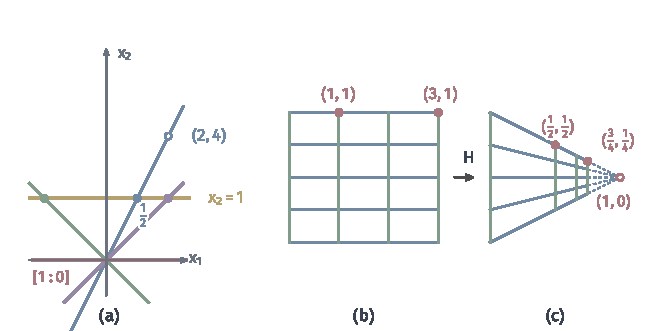
\includegraphics[width=112mm]{figures/04-spaces-measures-and-geometry/04-manifolds/matplotlib/lie-projective/figure.pdf}
  \caption{射影空间的仿射图与射影变换。(a)$\mathbb{RP}^1$的末分量图：过原点的直线与黄线$x_2=1$的交点给出坐标，蓝线是$[2:4]$，坐标为$\frac12$；红色水平线$[1:0]$不与黄线相交，是这张图的无穷远点。(b)平面上的方格，蓝线$v=$常数，绿线$u=$常数，红点是$(1,1)$与$(3,1)$。(c)方格在$\bm H$下的像（横向比例放大）：绿线仍是竖线，蓝线不再平行，延长后交于$(1,0)$。}
  \label{fig:lie-projective}
\end{BookInlineFigure}

在射影平面$\mathbb{RP}^2$中，非零系数向量$\bm\ell\in\mathbb R^3$确定直线$\{[\bm x]:\bm\ell^\top\bm x=0\}$，$\bm\ell$与它的非零倍数确定同一条直线。在$x_3=1$的图中它就是$\ell_1u+\ell_2v+\ell_3=0$。

两条平行线$u=0$与$u=1$的系数分别是$(1,0,0)^\top$与$(1,0,-1)^\top$。同时满足两个方程，第一个方程给出$x_1=0$，第二个方程再给出$x_3=0$，所以交点的齐次坐标是$[0:1:0]$，在这张图之外。平行线在射影平面中交于一个无穷远点。

\paragraph{射影变换}
可逆线性映射把过原点的直线映成过原点的直线，所以诱导出射影空间上的变换。

\begin{definition}[射影变换]
\label{def:lie-projective-transformation}
对$\bm H\in\mathrm{GL}(n+1,\mathbb R)$，映射$[\bm x]\mapsto[\bm H\bm x]$称为$\mathbb{RP}^n$上的\term{射影变换}（projective transformation）。
\end{definition}

它不依赖代表元，因为$\bm H(\lambda\bm x)=\lambda\bm H\bm x$；$\bm H\bm x\neq\bm0$由$\bm H$可逆保证。在仿射图中它是有理函数，因而光滑，逆变换由$\bm H^{-1}$给出，所以是微分同胚。$\bm H$与$c\bm H$（$c\neq0$）给出同一个变换，所以射影变换组成的群是$\mathrm{GL}(n+1,\mathbb R)$按非零数量矩阵取商，参数个数为$(n+1)^2-1$，平面的情形$n=2$有$8$个自由度。

射影变换保持点在线上的关系。若点按$\bm x'=\bm H\bm x$变换，令直线系数按$\bm\ell'=\bm H^{-\top}\bm\ell$变换，则
\[
\bm\ell'^\top\bm x'=\bm\ell^\top\bm H^{-1}\bm H\bm x=\bm\ell^\top\bm x,
\]
所以$\bm x$在$\bm\ell$上当且仅当$\bm x'$在$\bm\ell'$上。

它一般不保持长度、角度和平行。例如
\[
\bm H=\begin{bmatrix}1&0&0\\0&1&0\\1&0&1\end{bmatrix},\qquad
(u,v)\longmapsto\Bigl(\frac{u}{u+1},\frac{v}{u+1}\Bigr)\quad(u\neq-1).
\]
点$(1,1)$变成$(\frac12,\frac12)$，点$(3,1)$变成$(\frac34,\frac14)$。

这两个像点的连线延长后经过$(1,0)$，因为直线$v=1$上的点都是$\frac{v}{u+1}=\frac1{u+1}=1-\frac{u}{u+1}$，满足$v'=1-u'$。所有水平线$v=c$的像都经过$(1,0)$，图~\ref{fig:lie-projective}(b)(c)中平行的蓝线在像中汇聚到这一点。这个点是平行线在无穷远处交点的像：$\bm H(1,0,0)^\top=(1,0,1)^\top$。

直线$u=-1$上的点仍有合法的齐次像，只是像的第三分量为零，落到末分量图的无穷远处。所以“除以末分量”只能在它非零时进行，不能当作全局的线性运算。

刚体变换是射影变换的特例：式~\eqref{eq:lie-homogeneous-pose}中的$\bm T$底行为$(0,0,0,1)$，把末分量为$1$的点仍送到末分量为$1$的点，保持无穷远点组成的集合。由给定的点对应估计一个未知的$\bm H$，需要消去未知的比例并处理退化配置，这是第~\ref{chap:spatial-map-estimation}章的问题。

\subsection{Grassmann空间}
\label{sec:lie-grassmann}

射影空间研究$\mathbb R^{n+1}$中的一维子空间。数据分析中常常关心更高维的子空间，例如一组样本主要分布在哪个$k$维子空间附近。子空间本身是一个几何对象，但要计算它，通常得选一组基，把它记为矩阵；不同的基给出同一个子空间。

\paragraph{用基表示子空间}
设$\bm Y\in\mathbb R^{n\times k}$的列线性无关，它的列空间是一个$k$维子空间。若$\bm A\in\mathrm{GL}(k,\mathbb R)$，则$\bm Y\bm A$的各列是$\bm Y$各列的线性组合，并且仍线性无关，所以列空间不变。反过来，若$\bm Y,\bm Y'$列空间相同，则$\bm Y'$的每一列都能唯一地写成$\bm Y$各列的组合，即$\bm Y'=\bm Y\bm A$，且$\bm A$可逆。所以“同一子空间”恰好是$\mathrm{GL}(k,\mathbb R)$按右乘作用的轨道，这个对象因此可以用商来定义。

\begin{definition}[Grassmann空间]
\label{def:lie-grassmann}
$\mathbb R^n$中全体$k$维线性子空间组成的集合记为$\mathrm{Gr}(k,n)$，称为\term{Grassmann空间}（Grassmannian）。
\end{definition}

列满秩的$n\times k$矩阵组成$\mathbb R^{n\times k}$中的开集，记为$F$，$\mathrm{GL}(k,\mathbb R)$按$\bm A\cdot\bm Y=\bm Y\bm A^{-1}$在其上作用。作用是自由的：$\bm Y\bm A=\bm Y$与列满秩推出$\bm A=\bm I$。

作用也是适当的。设$K\subset F\times F$紧，若$(\bm Y\bm A^{-1},\bm Y)\in K$，记$\bm Y'=\bm Y\bm A^{-1}$，由列满秩解出
\[
\bm A=(\bm Y'^\top\bm Y')^{-1}\bm Y'^\top\bm Y,\qquad
\bm A^{-1}=(\bm Y^\top\bm Y)^{-1}\bm Y^\top\bm Y'.
\]
两个公式的右边在紧集$K$上连续，所以$\bm A$与$\bm A^{-1}$都有界，原像落在$\mathrm{GL}(k,\mathbb R)$的紧子集与$K$的投影之积内，又是闭集，从而是紧集。

由定理~\ref{thm:lie-quotient-manifold}，$\mathrm{Gr}(k,n)$是光滑流形，维数为$nk-k^2=k(n-k)$。$k=1$时它就是$\mathbb{RP}^{n-1}$，维数$n-1$。

\paragraph{用标准正交基表示}
计算中更常用标准正交基。满足$\bm Y^\top\bm Y=\bm I_k$的$n\times k$矩阵全体称为\term{Stiefel流形}（Stiefel manifold），记为$\mathrm{St}(k,n)$。与定理~\ref{thm:lie-orthogonal-group-manifold}的证明相同，约束$\bm Y^\top\bm Y=\bm I_k$取值于$\mathrm{Sym}(k)$且以$\bm I_k$为正则值，所以$\mathrm{St}(k,n)$的维数是$nk-k(k+1)/2$。

同一子空间的两组标准正交基只差一个正交矩阵，$\bm Y'=\bm Y\bm Q$，$\bm Q\in\mathrm O(k)$。紧群$\mathrm O(k)$的这一作用自由且适当，于是
\begin{equation}
 \mathrm{Gr}(k,n)\cong\mathrm{St}(k,n)/\mathrm O(k).
 \label{eq:lie-grassmann-stiefel}
\end{equation}
维数核对：
\[
nk-\frac{k(k+1)}2-\frac{k(k-1)}2=k(n-k),
\]
与上一段的结果一致。$k=n$时$\mathrm{St}(n,n)=\mathrm O(n)$，$\mathrm{Gr}(n,n)$只有一个点。

\paragraph{子空间与标架的区别}
标准正交基$\bm Y$称为一个标架，它比子空间多记录了$k(k-1)/2$个自由度，即在子空间内部怎样选取各轴。图~\ref{fig:lie-grassmann-frames}(a)中$\mathbb R^3$的一张平面对应两组不同的标架，它们是$\mathrm{St}(2,3)$中两个不同的点，却是$\mathrm{Gr}(2,3)$中同一个点。

消除这些自由度的一种方式是改用正交投影矩阵$\bm P=\bm Y\bm Y^\top$。对$\bm Q\in\mathrm O(k)$，
\[
(\bm Y\bm Q)(\bm Y\bm Q)^\top=\bm Y\bm Q\bm Q^\top\bm Y^\top=\bm Y\bm Y^\top,
\]
所以$\bm P$只依赖子空间；反过来，$\bm P$的列空间就是该子空间。于是$\mathrm{Gr}(k,n)$可以与秩为$k$的对称幂等矩阵一一对应，这个矩阵集合是
\[
\{\bm P:\bm P^\top=\bm P,\ \bm P^2=\bm P,\ \operatorname{tr}\bm P=k\}.
\]

切方向也要区分。在标架$\bm Y$处，Stiefel流形的切向量$\bm\Delta$满足$\bm Y^\top\bm\Delta+\bm\Delta^\top\bm Y=\bm0$。设$\bm Y_\perp$的列是正交补的一组标准正交基，切向量分解为
\[
\bm\Delta=\bm Y\bm\Omega+\bm Y_\perp\bm B,\qquad \bm\Omega^\top=-\bm\Omega .
\]

形如$\bm Y\bm\Omega$的方向只在子空间内部转动标架，不改变子空间，称为竖直方向；形如$\bm Y_\perp\bm B$（满足$\bm Y^\top\bm\Delta=\bm0$）的方向才真正把子空间推向别处，称为水平方向。水平方向组成的线性空间维数为$(n-k)k$，恰好是$\mathrm{Gr}(k,n)$的维数，可以作为子空间处切空间的具体表示。

取$n=3$，$k=2$，$\bm Y=[\bm e_1,\bm e_2]$。竖直方向和水平方向各取一个例子：
\[
\bm\Delta_v=[\bm e_2,\ -\bm e_1],\qquad
\bm\Delta_h=[\tfrac12\bm e_3,\ \bm0].
\]
前者对应$\bm\Omega=\begin{bmatrix}0&-1\\1&0\end{bmatrix}$，后者对应$\bm B=(\tfrac12,0)$，它把平面绕$\bm e_2$轴倾斜。图~\ref{fig:lie-grassmann-frames}(b)画出了这两种方向。

\begin{BookInlineFigure}
  \centering
  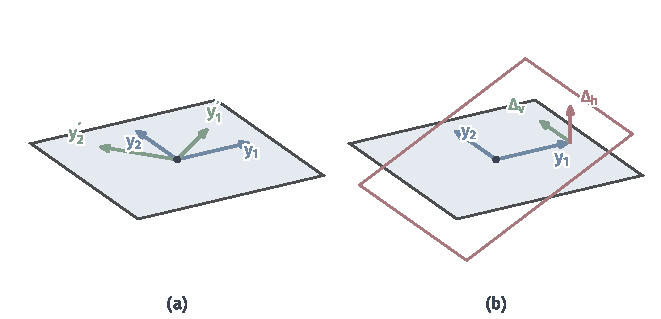
\includegraphics[width=112mm]{figures/04-spaces-measures-and-geometry/04-manifolds/matplotlib/lie-grassmann-frames/figure.pdf}
  \caption{$\mathbb R^3$中的平面与标架。(a)同一张平面的两组标准正交基，蓝色$\bm Y$与绿色$\bm Y\bm Q$相差平面内转动$38^\circ$，它们是$\mathrm{St}(2,3)$的两个点、$\mathrm{Gr}(2,3)$的同一个点。(b)标架$\bm Y=[\bm e_1,\bm e_2]$处的两种切向量。绿箭头是竖直方向$\bm\Delta_v$的第一列（画成$0.75$倍长），只转动标架；红箭头是水平方向$\bm\Delta_h$的第一列，把平面倾斜到红框所示的新平面。}
  \label{fig:lie-grassmann-frames}
\end{BookInlineFigure}

\paragraph{局部坐标}
子空间也有类似仿射图的坐标。若一个$k$维子空间与后$n-k$个坐标组成的子空间只交于零，它就有唯一的一组基写成$\begin{bmatrix}\bm I_k\\\bm B\end{bmatrix}$，$\bm B\in\mathbb R^{(n-k)\times k}$。$\bm B$的$k(n-k)$个元素就是这类子空间的坐标。$k=1$时它正是射影空间的首分量仿射图。不满足这个条件的子空间，换一组$k$个坐标的位置即可同样处理。

以正交约束或子空间为未知量的优化，要把这里的切方向、商结构与回到流形的更新方式结合起来，这是\BookChapterRef{chap:manifold-optimization}{卷五第25章“流形优化”}的内容；本节只说明这些未知量是什么对象、有多少自由度。

\section{本章小结}
\label{sec:lie-summary}

本章开头问：怎样说清一个计算“不受旋转影响”还是“随旋转同步变化”，以及怎样在只有三个自由度的旋转上做计算而不破坏约束。第一个问题的回答分两层。群只规定变换怎样复合：结合律、单位元和逆元保证变换可以接连施加和撤销，复合的次序一般不能交换。子群是对运算封闭的允许变换，而不是任意子集；同态保持复合，它的核记录丢失了哪些区分，像记录实际表示了哪些元素，元素个数相同的两个群未必同构。

群作用再规定每个变换怎样改变一个具体对象。同一个群可以作用在点、点云和图像上，公式各不相同，都要核对单位元与复合两条规则。轨道收集通过变换可以互相到达的对象，稳定子收集不改变给定对象的变换，二者分别是对象集合与群的子集，由陪集一一联系。在输入与输出的作用都给定后，不变映射在每条轨道上取常值，等变映射的输出按指定规则随输入变化；重心对置换不变、对旋转等变，距离矩阵对旋转不变、对置换在共轭作用下等变。不变是输出作用平凡时的等变，不变性也不保证保留了区分轨道所需的信息。

第二个问题由矩阵Lie群回答。$\mathrm{GL}(n,\mathbb R)$是开集，$\mathrm O(n)$与$\mathrm{SO}(n)$是正则水平集，乘法与求逆都光滑，左平移把单位元处的切空间搬到每一点。单位元处的切空间即Lie代数，可以做线性组合，交换子记录变换的不交换；它的元素是速度，不是群中的变换。矩阵指数由幂级数定义，把Lie代数方向变成单参数子群，并在单位元附近给出局部坐标，但一般既不单射也不满射。它只依赖群结构，与依赖度量的黎曼指数是两回事，只在$\mathrm{SO}(n)$配Frobenius度量这类特殊情形中吻合。

三维旋转没有全局无奇异的三参数坐标，这由$\mathrm{SO}(3)$的紧性直接推出。旋转矩阵直接作用于向量；轴角由Rodrigues公式给出，在半圈旋转与恒等旋转处有冗余，旋转向量在模长小于$\pi$的开球内是局部坐标；Euler角在万向节锁处秩下降，那是坐标的奇异而非旋转的退化。单位四元数以乘法完成复合，在每一点附近都给出正常坐标，代价是$q$与$-q$表示同一旋转，这一双覆盖不是额外的物理自由度。刚体位姿把旋转与平移合成$\mathrm{SE}(3)$，复合时前一次的平移要随后一次的旋转转动，方向不受平移影响；同一个齐次矩阵既可读作主动变换，也可读作坐标系换算。

最后，多种记录代表同一对象时，用群作用把同一轨道合并。商集合与商拓扑总能定义，但光滑结构需要条件：自由且适当的光滑作用给出维数为$\dim M-\dim G$的商流形，闭子群给出齐性空间，例如$\mathrm{SO}(3)/\mathrm{SO}(2)\cong S^2$；$\mathrm{SO}(2)$作用于平面的商有端点，无理旋转的商不是Hausdorff空间，都说明这些条件不能省略。射影空间合并非零倍数，用仿射图记录点、用可逆矩阵诱导射影变换；Grassmann空间合并张成同一子空间的不同基，标架比子空间多出的自由度可以用投影矩阵或水平方向消去。由点对应实际估计刚体变换与射影变换，在第~\ref{chap:spatial-map-estimation}章研究；正交矩阵与子空间上的优化算法留给卷五。


\chapter{空间映射估计}
\label{chap:spatial-map-estimation}

测量设备常常只给出相对的几何信息。测距仪报告两个标记点相隔多远，却不报告它们在哪个坐标系中；两台相机拍到同一组标记，各自记下自己的像素坐标，却不知道两套坐标之间怎样换算。这里有两类问题：只知道点与点之间的距离，能否给这些点安排坐标；知道两组点一一对应，能否求出把一组坐标送到另一组坐标的映射。两类问题都要先问观测究竟确定了什么，再谈怎样计算。

本章沿“可辨识性—坐标重构—映射估计”的顺序展开。第~\ref{sec:smap-identifiability}节说明距离对整体平移、旋转和反射一无所知，缺失距离还可能留下真正的形变自由度，固定参照只能消除前一类自由度。第~\ref{sec:smap-distance-reconstruction}节处理距离表：完整表经过平方和双中心化变成Gram矩阵，由谱分解读出能否实现、最少需要几维以及坐标本身；再研究指定维数下的近似、只观测部分距离时形状何时确定，以及测量误差怎样传到坐标。

第~\ref{sec:smap-map-estimation}节转向已知对应点的映射估计。先规定允许的映射族，再依次处理刚体、仿射和射影三种模型：刚体模型由质心消去平移、由交叉矩阵的奇异值分解求旋转；仿射模型用增广坐标化为线性最小二乘；射影模型在齐次坐标下只确定到一个非零倍数，代数残差与几何上的重投影误差需要分开评价。每种模型都逐项核对数据是否可满足、参数是否唯一、扰动下是否稳定。

本章把点之间的对应关系当作给定的输入，不讨论怎样从未标注的两组点中找出对应。旋转、位姿与射影空间的定义取自第~\ref{chap:lie-groups}章；以几何误差为目标的迭代求解属于卷五的光滑优化。有限个点的另一类问题，即把样本看成某个未知流形上的采样、恢复它的局部几何与拓扑，是第~\ref{chap:manifold-recovery}章的任务。

\section{相对观测的可辨识性}
\label{sec:smap-identifiability}

在计算任何坐标或映射之前，先要弄清观测能够确定什么。一组测量即使完全没有误差，也可能对某些量毫无约束：把整幅图平移一下，所有距离都不变，距离表当然无法告诉我们原点在哪里。本节先区分两类相对观测，再把观测不能辨认的自由度分成两种：一种来自坐标系的任意选择，另一种来自观测本身的缺失。

\paragraph{两类相对观测}

第一类观测只涉及点与点之间的关系。给定点标签集合$V=\{1,\ldots,n\}$和已观测的点对集合$E$，对每个$\{i,j\}\in E$测得一个距离$d_{i,j}\geq0$。未知的是坐标$\bm x_1,\ldots,\bm x_n\in\mathbb R^d$，要求它们满足
\[
 \lVert\bm x_i-\bm x_j\rVert_2=d_{i,j},\qquad\{i,j\}\in E .
\]
$E$包含全部点对时称距离表完整，否则称为部分距离。这里的数据只有标签与数，没有任何外部坐标。

第二类观测涉及同一组物理点在两种坐标表示下的记录。对每个$i$，已知源坐标$\bm x_i\in\mathbb R^d$与目标坐标$\bm y_i\in\mathbb R^m$，并且知道它们描述同一个点。未知的是把源坐标送到目标坐标的映射$f$，要求$f(\bm x_i)\approx\bm y_i$。两类问题的未知量不同：前者的未知量是$n$个点的坐标，共$nd$个数；后者的未知量是一个映射，点越多，对它的约束越多。

\paragraph{整体欧氏自由度}

先看距离不能辨认什么。取正交矩阵$\bm Q\in\mathrm O(d)$和向量$\bm b\in\mathbb R^d$，令$\bm x_i'=\bm Q\bm x_i+\bm b$。差向量变为$\bm x_i'-\bm x_j'=\bm Q(\bm x_i-\bm x_j)$，正交矩阵保持长度，所以每一对点的距离都不变。也就是说，平移、旋转和反射作用于整组点以后，任何距离观测都看不出区别。

\begin{definition}[合同的点配置]
\label{def:smap-congruent}
两组点$\bm x_1,\ldots,\bm x_n$与$\bm x_1',\ldots,\bm x_n'\in\mathbb R^d$称为\term{合同}（congruent），如果存在$\bm Q\in\mathrm O(d)$和$\bm b\in\mathbb R^d$，使$\bm x_i'=\bm Q\bm x_i+\bm b$对所有$i$成立。
\end{definition}

由上一段的计算，合同的配置给出同一张距离表。因此距离观测最多只能把点配置确定到合同的程度，这一限制与测量是否完整、是否精确都无关。平移有$d$个参数，$\mathrm O(d)$的每个连通分支有$d(d-1)/2$个参数，所以合同带来$d(d+1)/2$个连续自由度，外加一个反射的二选一。平面上是$3$个连续自由度，空间中是$6$个。

反过来，完整距离表是否把配置确定到合同为止？第~\ref{sec:smap-full-distance}节会证明答案是肯定的：两组点的全部距离相同，它们就合同。这说明对完整距离表而言，合同是唯一的不确定性，坐标重构的任务是在合同意义下找出配置。

\paragraph{缺失观测的形变自由度}

观测不完整时，不确定性可能多于合同。在平面上取单位正方形的四个顶点，只测四条边长，都等于$1$，不测两条对角线。把正方形压成内角为$\theta$的菱形，四条边长仍是$1$，但两条对角线长分别变为$2\sin(\theta/2)$与$2\cos(\theta/2)$。$\theta\neq\pi/2$时对角线与正方形不同，所以菱形与正方形不合同，却满足全部观测。

这里的自由度来自观测不足，可以用计数来理解。平面上$n$个点有$2n$个坐标，扣去合同的$3$个自由度，形状本身还有$2n-3$个自由度；$n=4$时为$5$个，四个边长约束一般只能消去其中四个，剩下的一个就是菱形的内角。计数只给出必要条件，约束够多也未必确定形状，第~\ref{sec:smap-partial-distance}节将用具体例子说明这一点。

\paragraph{固定参照的作用}

为了得到一组具体坐标，常常人为固定参照。在平面上可以规定$\bm x_1=\bm0$，$\bm x_2$位于第一坐标轴正半轴上，$\bm x_3$位于上半平面。这三条规定恰好消去平移、旋转和反射：任何配置都与唯一一个满足规定的配置合同，只要$\bm x_1,\bm x_2,\bm x_3$不共线。

但规定只能消去约定上的自由度。回到菱形的例子，取$\bm x_1=\bm0$、$\bm x_2=(1,0)^\top$，并把第四个点放在上半平面，内角$\theta$仍然可以连续变化，四个边长仍然成立。形变自由度是由缺失的观测造成的，再多的坐标约定也补不出缺失的对角线长度。

还要区分约定与观测。若某些点的绝对位置是用仪器测出来的，例如卫星定位给出的锚点坐标，它们就是额外的观测，可能与距离数据相互矛盾，需要进入拟合残差；只有任意选取、不影响距离的规定，才是消去合同自由度的约定。第二类问题中也有对应的区分：两套坐标系都已给定，映射本身没有约定上的自由度，但必须事先选定映射族，第~\ref{sec:smap-correspondence-models}节将说明这一点。

\section{距离观测的坐标重构}
\label{sec:smap-distance-reconstruction}

上一节说明，距离最多把点配置确定到合同为止。本节在这个限度内研究重构：完整距离表在什么条件下来自欧氏点、最少需要几维、怎样写出坐标；维数受限时怎样近似；只观测部分距离时形状是否仍然确定；以及测量误差会怎样传到坐标。比较两组坐标时，总要先消去整体平移与正交变换，否则相差一个旋转的两组正确坐标也会被误判为不同。

\subsection{完整距离的欧氏实现}
\label{sec:smap-full-distance}

设$n$个点两两之间的距离全部已知，排成矩阵$\bm D=[d_{i,j}]\in\mathbb R^{n\times n}$。任何来自点的距离表都满足三条基本要求：各项非负，$d_{i,j}=d_{j,i}$，对角元$d_{i,i}=0$。下面始终假定输入满足这三条，并记逐项平方后的矩阵为$\bm\Delta=[\delta_{i,j}]$，$\delta_{i,j}=d_{i,j}^2$。问题是：是否存在$\bm x_1,\ldots,\bm x_n\in\mathbb R^d$，使$\lVert\bm x_i-\bm x_j\rVert_2^2=\delta_{i,j}$对所有$i,j$成立？若存在，称$\bm\Delta$\term{欧氏可实现}（Euclidean realizable），所取的点称为它的一个实现。

\paragraph{从坐标到Gram矩阵}

先从已知坐标出发，看平方距离与内积怎样联系。把各点按行排成$\bm X\in\mathbb R^{n\times d}$，第$i$行为$\bm x_i^\top$，Gram矩阵$\bm G=\bm X\bm X^\top$记录两两内积$g_{i,j}=\bm x_i^\top\bm x_j$。展开平方距离，
\begin{equation}
 \delta_{i,j}=\lVert\bm x_i\rVert_2^2+\lVert\bm x_j\rVert_2^2-2\bm x_i^\top\bm x_j=g_{i,i}+g_{j,j}-2g_{i,j}.
 \label{eq:smap-distance-gram}
\end{equation}
写成矩阵，记$\bm g=(g_{1,1},\ldots,g_{n,n})^\top$、$\bm1$为全一向量，就是$\bm\Delta=\bm g\bm1^\top+\bm1\bm g^\top-2\bm G$。

反方向不能直接解出$\bm G$。距离不依赖原点，内积却依赖：整组点平移后，$\bm\Delta$不变而$\bm G$改变。所以要先约定原点，最自然的选择是质心。令
\begin{equation}
 \bm J=\bm I_n-\frac1n\bm1\bm1^\top ,
 \label{eq:smap-centering-matrix}
\end{equation}
它对称，满足$\bm J^2=\bm J$与$\bm J\bm1=\bm0$，是到$\bm1$的正交补上的正交投影。$\bm J\bm X$从每一行减去各点的平均坐标，所以$\bm J\bm X$的各行就是以质心为原点的坐标。

用$\bm J$左右夹乘$\bm\Delta$。由$\bm J\bm1=\bm0$，$\bm J\bm g\bm1^\top\bm J$与$\bm J\bm1\bm g^\top\bm J$都是零矩阵，只剩
\begin{equation}
 -\frac12\bm J\bm\Delta\bm J=\bm J\bm G\bm J=(\bm J\bm X)(\bm J\bm X)^\top .
 \label{eq:smap-double-centering}
\end{equation}
右端正是中心化坐标的Gram矩阵。这一运算称为\term{双中心化}（double centering）：左乘$\bm J$消去行上的均值项，右乘消去列上的均值项，把平方距离转成以质心为原点的内积。下面记$\bm B=-\frac12\bm J\bm\Delta\bm J$，它对任何对称零对角的$\bm\Delta$都有定义，不必事先知道$\bm\Delta$来自点。

\paragraph{可实现的判据}

若$\bm\Delta$可实现，由式~\eqref{eq:smap-double-centering}，$\bm B$是一个Gram矩阵，因而半正定：$\bm c^\top\bm B\bm c=\lVert(\bm J\bm X)^\top\bm c\rVert_2^2\geq0$。要证明半正定也是充分的，需要确认双中心化没有丢掉信息，即零对角的对称矩阵由它的双中心化唯一确定。

\begin{lemma}[双中心化的核]
\label{lem:smap-double-centering-kernel}
设$\bm H\in\mathbb R^{n\times n}$对称且$\bm J\bm H\bm J=\bm0$，则存在$\bm a\in\mathbb R^n$使$\bm H=\bm a\bm1^\top+\bm1\bm a^\top$。若还有$h_{i,i}=0$对所有$i$成立，则$\bm H=\bm0$。
\end{lemma}
\begin{proof}
记$\bm m=\frac1n\bm H\bm1$，$\mu=\frac1{n^2}\bm1^\top\bm H\bm1$。把$\bm J=\bm I-\frac1n\bm1\bm1^\top$代入$\bm J\bm H\bm J=\bm0$并展开，
\[
 \bm H-\bm1\bm m^\top-\bm m\bm1^\top+\mu\bm1\bm1^\top=\bm0 .
\]
取$\bm a=\bm m-\frac\mu2\bm1$，即得$\bm H=\bm a\bm1^\top+\bm1\bm a^\top$。此时$h_{i,i}=2a_i$，零对角迫使$\bm a=\bm0$，于是$\bm H=\bm0$。
\end{proof}

\begin{theorem}[欧氏可实现的判据]
\label{thm:smap-realizability}
设$\bm\Delta\in\mathbb R^{n\times n}$对称、零对角，$\bm B=-\frac12\bm J\bm\Delta\bm J$。则$\bm\Delta$是某组欧氏点的平方距离矩阵，当且仅当$\bm B$半正定。此时实现所需的最小维数等于$r=\operatorname{rank}\bm B$，并且可以取
\begin{equation}
 \bm Y=\bm Q_r\bm\Lambda_r^{1/2}\in\mathbb R^{n\times r},
 \label{eq:smap-classical-scaling}
\end{equation}
其中$\bm\Lambda_r$是$\bm B$的$r$个正特征值组成的对角矩阵，$\bm Q_r$的列是对应的标准正交特征向量。
\end{theorem}
\begin{proof}
必要性已在上面说明。设$\bm B$半正定，由对称矩阵的谱分解，$\bm B=\bm Q_r\bm\Lambda_r\bm Q_r^\top$，于是式~\eqref{eq:smap-classical-scaling}的$\bm Y$满足$\bm Y\bm Y^\top=\bm B$。由$\bm B\bm1=\bm0$得$\lVert\bm Y^\top\bm1\rVert_2^2=\bm1^\top\bm B\bm1=0$，即$\bm Y$的各行已经中心化，$\bm J\bm Y=\bm Y$。

记$\bm\Delta'$为$\bm Y$各行的平方距离矩阵。由式~\eqref{eq:smap-double-centering}，$-\frac12\bm J\bm\Delta'\bm J=\bm Y\bm Y^\top=\bm B$，所以$\bm H=\bm\Delta-\bm\Delta'$对称、零对角且$\bm J\bm H\bm J=\bm0$。由引理~\ref{lem:smap-double-centering-kernel}，$\bm H=\bm0$，即$\bm Y$实现了$\bm\Delta$。

最后看维数。任何$\mathbb R^k$中的实现，中心化后的Gram矩阵就是$\bm B$，而它是$n\times k$矩阵与其转置之积，秩不超过$k$，故$k\geq r$；上面的构造又在$k=r$时达到。$r=0$时所有点重合。
\end{proof}

这一判据与谱分解构造合称\term{经典多维尺度}（classical multidimensional scaling）。所用的对称矩阵谱分解可参考\BookChapterRef{chap:eigen-spectral-decomposition}{卷二第4章“特征值与谱分解”}。计算步骤是：逐项平方得$\bm\Delta$，双中心化得$\bm B$，求$\bm B$的特征值与特征向量，检查有无负特征值，再按式~\eqref{eq:smap-classical-scaling}写出坐标，最后用重构坐标重新计算距离与原表核对。

\paragraph{坐标的唯一性}

谱分解中特征向量可以变号，重特征值时特征空间内部还可以换基，所以式~\eqref{eq:smap-classical-scaling}给出的坐标并不唯一。下面的定理说明，这些差别恰好是正交变换，并且任何两个同维实现都只差一个合同。

\begin{theorem}[完整距离确定合同类]
\label{thm:smap-full-distance-congruence}
设$\bm x_1,\ldots,\bm x_n$与$\bm x_1',\ldots,\bm x_n'\in\mathbb R^d$的两两距离全部相同，则两组点合同。更具体地，以各自质心为原点后，存在$\bm Q\in\mathrm O(d)$使$\bm x_i'-\overline{\bm x}'=\bm Q(\bm x_i-\overline{\bm x})$对所有$i$成立。
\end{theorem}
\begin{proof}
记$\bm z_i=\bm x_i-\overline{\bm x}$、$\bm z_i'=\bm x_i'-\overline{\bm x}'$。由式~\eqref{eq:smap-double-centering}，两组中心化坐标的Gram矩阵都等于同一个$\bm B$，即$\bm z_i^\top\bm z_j=\bm z_i'^\top\bm z_j'$对所有$i,j$成立。

于是对任意系数$\bm c\in\mathbb R^n$，$\lVert\sum_ic_i\bm z_i\rVert_2^2=\bm c^\top\bm B\bm c=\lVert\sum_ic_i\bm z_i'\rVert_2^2$。取$S=\operatorname{span}\{\bm z_i\}$、$S'=\operatorname{span}\{\bm z_i'\}$，规定$L(\sum_ic_i\bm z_i)=\sum_ic_i\bm z_i'$。若两组系数给出$S$中同一向量，它们的差$\bm c$使$\sum_ic_i\bm z_i=\bm0$，由上式$\sum_ic_i\bm z_i'=\bm0$，所以$L$是良定义的线性映射，并且保持长度。

保长的线性映射是单射，所以$\dim S'=\dim S$，正交补$S^\perp$与$S'^\perp$维数也相同。在两个正交补中各取一组标准正交基，把前者逐个送到后者，就把$L$延拓为$\mathbb R^d$上保长的线性映射$\bm Q$，即正交矩阵，并且$\bm Q\bm z_i=\bm z_i'$。
\end{proof}

这一定理兑现了第~\ref{sec:smap-identifiability}节的论断：对完整距离表，合同是唯一的不确定性。$\bm\Lambda_r$的特征值互不相同时，式~\eqref{eq:smap-classical-scaling}中特征向量的选取只差各列的符号，对应沿各坐标轴的反射；有重特征值时，相应的坐标轴可以在特征空间内任意旋转。

\paragraph{实现与不可实现的例子}

\begin{example}[三个点的重构]
\label{ex:smap-three-point-mds}
取$\bm x_1=(-1,0)^\top$、$\bm x_2=(0,1)^\top$、$\bm x_3=(1,0)^\top$，平方距离为$\delta_{1,2}=\delta_{2,3}=2$、$\delta_{1,3}=4$。记一般的$\delta_{1,2}=\delta_{2,3}=a$、$\delta_{1,3}=b$，由对称性可以直接读出$\bm B$的特征向量：$\bm1$对应特征值$0$；对$\bm v=(1,0,-1)^\top/\sqrt2$，由$\bm J\bm v=\bm v$得$\bm v^\top\bm B\bm v=-\frac12\bm v^\top\bm\Delta\bm v=b/2$；对$\bm w=(1,-2,1)^\top/\sqrt6$，同样算得$\bm w^\top\bm B\bm w=(4a-b)/6$。

代入$a=2$、$b=4$，正特征值为$2$与$2/3$，所以精确重构恰好需要二维。由式~\eqref{eq:smap-classical-scaling}，重构坐标的两列为$\sqrt2\,\bm v=(1,0,-1)^\top$与$\sqrt{2/3}\,\bm w=(1,-2,1)^\top/3$，三个点是$(1,1/3)$、$(0,-2/3)$、$(-1,1/3)$。它们两两的平方距离为$1+1=2$、$1+1=2$、$4+0=4$，与原表一致。原配置平移到质心后为$(-1,-1/3)$、$(0,2/3)$、$(1,-1/3)$，重构结果恰是它旋转$180^\circ$的结果，与原配置合同；特征向量取相反的符号，就得到中心化的原配置本身。
\end{example}

\begin{example}[违反三角不等式的距离表]
\label{ex:smap-nonrealizable}
取$d_{1,2}=d_{2,3}=1$、$d_{1,3}=3$，即$a=1$、$b=9$。按上例的公式，$\bm B$的特征值为$9/2$、$(4-9)/6=-5/6$与$0$，出现负特征值，所以这张表在任何维数的欧氏空间中都不可实现。这与直接观察一致：$3>1+1$违反三角不等式。负特征值的特征向量$(1,-2,1)^\top$指出问题出在中间点相对两端的位置上。
\end{example}

\subsection{低维坐标重构}
\label{sec:smap-low-dimension}

实际中常常指定维数$k$，例如要在平面上画出点的分布，而$\bm B$的秩可能大于$k$；含误差的距离表还可能让$\bm B$出现负特征值，根本不可实现。这时只能求近似坐标$\bm Y\in\mathbb R^{n\times k}$。近似必须先说明比较什么，本小节先以Gram矩阵为比较对象，再看距离上的误差。

\paragraph{Gram矩阵的最优截断}

以Frobenius范数比较Gram矩阵，问题是在秩不超过$k$的半正定矩阵中找离$\bm B$最近的一个。$\bm B$半正定时，它的谱分解就是奇异值分解，截断到前$k$个特征值即得最优解，这是最佳低秩逼近定理的直接推论，可参考\BookChapterRef{chap:matrix-approximation}{卷二第15章“矩阵逼近”}。$\bm B$有负特征值时还要多一步：负谱部分对任何半正定近似都只会增加误差。

\begin{theorem}[半正定低秩近似]
\label{thm:smap-psd-truncation}
设$\bm B$对称，特征值$\lambda_1\geq\cdots\geq\lambda_n$，特征向量为标准正交的$\bm q_1,\ldots,\bm q_n$。令$p$为正特征值的个数，$k'=\min(k,p)$，$\bm B_k=\sum_{l\leq k'}\lambda_l\bm q_l\bm q_l^\top$。则对一切秩不超过$k$的半正定矩阵$\bm X$，
\[
 \lVert\bm B-\bm X\rVert_{\mathrm F}^2\geq\lVert\bm B-\bm B_k\rVert_{\mathrm F}^2=\sum_{l=k'+1}^{p}\lambda_l^2+\sum_{\lambda_l<0}\lambda_l^2 .
\]
\end{theorem}
\begin{proof}
把$\bm B$分成正部与负部：
\begin{equation*}
\bm B_+=\sum_{\lambda_l>0}\lambda_l\bm q_l\bm q_l^\top,\qquad\bm B_-=\sum_{\lambda_l<0}(-\lambda_l)\bm q_l\bm q_l^\top,
\end{equation*}
二者都半正定，$\bm B=\bm B_+-\bm B_-$，且由特征向量正交，$\bm B_+\bm B_-=\bm0$。对半正定的$\bm X$展开，
\[
 \lVert\bm B_+-\bm X-\bm B_-\rVert_{\mathrm F}^2
 =\lVert\bm B_+-\bm X\rVert_{\mathrm F}^2+\lVert\bm B_-\rVert_{\mathrm F}^2+2\operatorname{tr}(\bm X\bm B_-),
\]
这里用了$\operatorname{tr}(\bm B_+\bm B_-)=0$。两个半正定矩阵之积的迹非负：写$\bm B_-=\bm C\bm C^\top$，则$\operatorname{tr}(\bm X\bm B_-)=\operatorname{tr}(\bm C^\top\bm X\bm C)\geq0$。

所以$\lVert\bm B-\bm X\rVert_{\mathrm F}^2\geq\lVert\bm B_+-\bm X\rVert_{\mathrm F}^2+\lVert\bm B_-\rVert_{\mathrm F}^2$。$\bm B_+$半正定，由最佳低秩逼近定理，秩不超过$k$时$\lVert\bm B_+-\bm X\rVert_{\mathrm F}^2\geq\sum_{l=k'+1}^p\lambda_l^2$，等号在$\bm X=\bm B_k$时取到；而$\bm X=\bm B_k$时$\operatorname{tr}(\bm B_k\bm B_-)=0$，上面的不等式都取等号。
\end{proof}

于是低维坐标取$\bm Y_k=\bm Q_{k'}\bm\Lambda_{k'}^{1/2}$，即只保留前$k'$个正特征值对应的列。它仍然中心化，因为每个保留的特征向量都与$\bm1$正交。负特征值被舍弃，舍弃量$\sum_{\lambda_l<0}\lambda_l^2$应与测量误差的大小比较：若它远大于误差能解释的范围，问题出在数据或模型上，而不是维数选小了。

\paragraph{距离上的误差}

Gram矩阵的误差并不直接说明距离差了多少，需要单独计算。设$\bm\Delta$可实现，$\bm Y=\bm Q_r\bm\Lambda_r^{1/2}$是它的中心化实现。$\bm Y_k$恰好是$\bm Y$的前$k$列，相当于把每个点正交投影到前$k$个坐标轴张成的子空间上。正交投影不增加长度，所以每一对点的距离只会缩短：$\lVert\widetilde{\bm y}_i-\widetilde{\bm y}_j\rVert_2\leq d_{i,j}$。

缩短的总量可以精确算出。对中心化的点，$\sum_{i<j}\lVert\bm y_i-\bm y_j\rVert_2^2=n\sum_i\lVert\bm y_i\rVert_2^2=n\operatorname{tr}\bm B$，这只需展开平方并用$\sum_i\bm y_i=\bm0$。对截断坐标同样有$\sum_{i<j}\widetilde\delta_{i,j}=n\operatorname{tr}\bm B_k$，相减得
\[
 \sum_{i<j}\bigl(\delta_{i,j}-\widetilde\delta_{i,j}\bigr)=n\sum_{l>k}\lambda_l .
\]
注意这里是特征值之和，而Gram误差的平方是特征值的平方和。两种误差都由舍弃的谱决定，但不是同一个量。

\begin{example}[三个点的一维近似]
\label{ex:smap-one-dimensional}
回到例~\ref{ex:smap-three-point-mds}，取$k=1$，只保留特征值$2$。一维坐标为$(1,0,-1)$，两端距离仍为$2$，中间点到两端的距离由$\sqrt2$缩成$1$。Gram误差为舍弃的特征值$2/3$；平方距离的总缩短量为$(2-1)+(2-1)+0=2$，恰为$n\lambda_2=3\cdot2/3$。
\end{example}

\paragraph{最优性依赖目标}

谱截断在Gram矩阵的Frobenius误差下最优，不等于在一切几何准则下最优。常用的另一种准则直接比较距离，称为应力：$\sum_{i<j}(\lVert\widetilde{\bm y}_i-\widetilde{\bm y}_j\rVert_2-d_{i,j})^2$。在上例中，截断坐标的应力为$2(\sqrt2-1)^2=2(3-2\sqrt2)\approx0.343$。

改取一维坐标$(-s,0,s)$，应力为$2(s-\sqrt2)^2+(2s-2)^2$，对$s$求导令其为零，得$s=(2+\sqrt2)/3\approx1.138$。代回去，$s-\sqrt2=(2-2\sqrt2)/3$，$2s-2=(2\sqrt2-2)/3$，应力为$3\cdot4(\sqrt2-1)^2/9=4(3-2\sqrt2)/3\approx0.229$，比截断坐标小。截断坐标把两端拉得太远、中间缩得太多，而应力准则愿意把各对距离的误差摊平。应力关于坐标不是凸的，一般需要迭代优化，而不能由一次谱分解得到。

\subsection{部分距离的重构}
\label{sec:smap-partial-distance}

许多测量只能给出部分点对的距离，例如传感器只能测到通信范围内的邻居。把已观测的点对看作边，就得到\term{观测图}（observation graph）$\mathcal G=(V,E)$；图的基本概念可参考\BookChapterRef{chap:graph-objects}{卷三第1章“图与连接结构”}。观测图不连通时，不同分量之间没有任何约束，各分量可以独立地移动，这是显然的；下面两个例子说明，连通也远远不够。

\paragraph{连通而形状不定}

在平面上取三个点，只观测$d_{1,2}=d_{2,3}=1$。观测图是一条路径，是连通的。但$\bm x_2$处的夹角可以任意选取：$\bm x_1$与$\bm x_3$都在以$\bm x_2$为圆心的单位圆上，它们的距离可以是$[0,2]$中的任何值。不同的夹角给出互不合同的配置，所以连通不保证形状确定。

\paragraph{局部确定而全局不唯一}

为了区分两种“确定”，先给出定义。设$\bm x_1,\ldots,\bm x_n\in\mathbb R^d$满足观测图$\mathcal G$上的全部距离，称它是一个实现。

\begin{definition}[局部刚性与全局刚性]
\label{def:smap-rigidity}
若存在$\eta>0$，使得每个满足同一组观测距离、且$\lVert\bm x_i'-\bm x_i\rVert_2<\eta$对所有$i$成立的实现都与原实现合同，则称原实现\term{局部刚性}（locally rigid）。若满足观测距离的每个实现都与它合同，则称它\term{全局刚性}（globally rigid）。
\end{definition}

取平面上$\bm x_1=(0,0)^\top$、$\bm x_2=(2,0)^\top$、$\bm x_3=(1,1)^\top$、$\bm x_4=(1,-2)^\top$，观测除$\{3,4\}$外的五对距离：$d_{1,2}=2$，$d_{1,3}=d_{2,3}=\sqrt2$，$d_{1,4}=d_{2,4}=\sqrt5$。这是两个共用边$\{1,2\}$的三角形。

先看局部刚性。三角形的三边确定它到合同为止，所以$\bm x_1,\bm x_2,\bm x_3$整体只能作合同变换；在此基础上，$\bm x_4$到$\bm x_1,\bm x_2$的距离给定，它只能落在两个圆的两个交点之一，即直线$\bm x_1\bm x_2$的两侧各一个。两个交点相距$4$，小范围的扰动不能从一个跳到另一个，所以原实现局部刚性。

再看全局。把$\bm x_4$关于直线$\bm x_1\bm x_2$反射到$(1,2)^\top$，五个观测距离都不变，未观测的$d_{3,4}$却由$3$变成$1$。两个实现互不合同，所以原实现不是全局刚性的。局部确定只排除了附近的连续形变，不排除远处另有一个离散的解。

\paragraph{缺边、不相容与含噪}

固定维数$d$，并按第~\ref{sec:smap-identifiability}节的方式约定参照以消去合同自由度之后，部分距离问题有三种不同的困难。缺边可能使解不唯一，如上面的路径和两个三角形；观测不相容时根本无解，例如三个点的三条观测边长为$1$、$1$、$3$；观测含噪时一般也无精确解，只能在已观测的边上度量偏差。

含噪时自然的做法是只对已观测的边建立残差，例如
\[
 \sum_{\{i,j\}\in E}\bigl(\lVert\bm x_i-\bm x_j\rVert_2-d_{i,j}\bigr)^2 ,
\]
或用平方距离之差代替距离之差。未观测的点对不进入目标，因为对它们没有任何数据。这类目标关于坐标不是凸的，可能有多个局部极小，对应的正是上面的离散多解；其求解属于迭代优化。

\paragraph{不能把缺失填成零}

把缺失的距离填零，再套用第~\ref{sec:smap-full-distance}节的谱重构，是常见的错误。零距离不是“未知”，而是断言两点重合。在路径的例子中填$d_{1,3}=0$，得到完整表$\delta_{1,2}=\delta_{2,3}=1$、$\delta_{1,3}=0$，按例~\ref{ex:smap-three-point-mds}的公式，$a=1$、$b=0$，$\bm B$的特征值为$(4a-b)/6=2/3$与$b/2=0$，表是可实现的：$\bm x_1=\bm x_3$，链被完全折叠。

谱重构会毫无警告地给出这个配置，好像形状已经确定，实际上它只是无穷多个可行形状中被错误的数据选中的一个。填入其他猜测值同样会选出某个特定形状。所以缺失距离只能作为“无约束”处理，或者在明确的附加假设下另行估计，而不能伪装成观测。

\subsection{坐标重构的稳定性}
\label{sec:smap-reconstruction-stability}

距离表总带有测量误差。本小节先研究完整表上的误差怎样经过平方、双中心化和谱分解传到坐标，再说明部分距离为什么需要另作分析。所用的特征值与特征子空间扰动界取自\BookChapterRef{chap:condition-and-spectral-perturbation}{卷二第7章“条件数与谱扰动”}：对称矩阵受对称扰动$\bm E$时，每个按降序配对的特征值至多移动$\lVert\bm E\rVert_2$（Weyl界）；若前$k$个特征值与其余特征值之间有间隔$g$，且$\lVert\bm E\rVert_2\leq g/2$，前$k$个特征向量张成的子空间最大主夹角的正弦不超过$2\lVert\bm E\rVert_2/g$（Davis--Kahan界）。

\paragraph{从距离误差到Gram误差}

设观测的平方距离表为$\widetilde{\bm\Delta}=\bm\Delta+\bm E$，$\bm E$对称、零对角。双中心化是线性的，$\widetilde{\bm B}-\bm B=-\frac12\bm J\bm E\bm J$。$\bm J$是正交投影，谱范数为$1$，所以
\[
 \lVert\widetilde{\bm B}-\bm B\rVert_2\leq\frac12\lVert\bm E\rVert_2 .
\]
注意误差是加在平方距离上的：若距离本身有误差$\varepsilon_{i,j}$，平方距离的误差为$2d_{i,j}\varepsilon_{i,j}+\varepsilon_{i,j}^2$，长距离上的同样误差会被放大。

\begin{theorem}[完整距离表的谱扰动]
\label{thm:smap-mds-perturbation}
在上述记号下，设$\lambda_1\geq\cdots\geq\lambda_n$与$\widetilde\lambda_1\geq\cdots\geq\widetilde\lambda_n$分别是$\bm B$与$\widetilde{\bm B}$的特征值，则$|\widetilde\lambda_l-\lambda_l|\leq\frac12\lVert\bm E\rVert_2$。若$g=\lambda_k-\lambda_{k+1}>0$且$\lVert\bm E\rVert_2\leq g$，则两者前$k$个特征向量张成的子空间满足$\sin\theta_{\max}\leq\lVert\bm E\rVert_2/g$。
\end{theorem}
\begin{proof}
对$\bm B$与扰动$\widetilde{\bm B}-\bm B$分别应用Weyl界与Davis--Kahan界，扰动的谱范数不超过$\frac12\lVert\bm E\rVert_2$；条件$\lVert\bm E\rVert_2\leq g$保证$\frac12\lVert\bm E\rVert_2\leq g/2$，代入$2\cdot\frac12\lVert\bm E\rVert_2/g$即得。
\end{proof}

\paragraph{谱隙与小特征值}

定理分两层说明误差的去向。特征值本身稳定，误差至多为$\frac12\lVert\bm E\rVert_2$。坐标轴的方向取决于谱隙：相邻特征值接近时，很小的误差就能让坐标轴在相应的特征空间内大幅转动，这与重特征值时坐标轴本来就不唯一是同一现象的两面。

坐标的长度还要再经过开方。第$l$列坐标按$\sqrt{\lambda_l}$缩放，而
\[
 \bigl|\sqrt{\widetilde\lambda_l}-\sqrt{\lambda_l}\bigr|=\frac{|\widetilde\lambda_l-\lambda_l|}{\sqrt{\widetilde\lambda_l}+\sqrt{\lambda_l}}\leq\frac{|\widetilde\lambda_l-\lambda_l|}{\sqrt{\lambda_l}} ,
\]
特征值越小，相对误差越大。更严重的是，误差与小特征值同量级时，$\widetilde\lambda_l$可能变成负数，这个方向就整个丢失了。

\begin{example}[几乎共线的三个点]
\label{ex:smap-near-collinear}
取$\bm x_1=(-1,0)^\top$、$\bm x_2=(0,h)^\top$、$\bm x_3=(1,0)^\top$，$h=0.1$。这时$a=\delta_{1,2}=\delta_{2,3}=1.01$，$b=\delta_{1,3}=4$，由例~\ref{ex:smap-three-point-mds}的公式，特征值为$b/2=2$与$(4a-b)/6=2h^2/3\approx0.0067$。

设$d_{1,3}$被测成$2.02$，只有$1\%$的误差，于是$\widetilde\delta_{1,3}=4.0804$。第二个特征值变为$(4.04-4.0804)/6\approx-0.0067$，由正变负。事实上$2.02>2\sqrt{1.01}\approx2.0100$已违反三角不等式，表在任何维数中都不可实现。第一个特征值只从$2$变为$2.0402$，相对变化约$2\%$；纵向那个高为$0.1$的坐标则完全丢失。这里$\bm E$只有$(1,3)$、$(3,1)$两项$0.0804$，$\lVert\bm E\rVert_2=0.0804$，两个特征值的变化都在Weyl界$0.0402$之内。
\end{example}

\paragraph{比较坐标前消去合同}

评价重构误差时，不能直接比较$\widetilde{\bm Y}$与真实坐标$\bm X$的各个分量：即使距离完全精确，重构也只确定到合同为止。正确的做法是先把两组坐标都平移到质心，再求
\[
 \min_{\bm Q\in\mathrm O(d)}\lVert\widetilde{\bm Y}-\bm X\bm Q\rVert_{\mathrm F},
\]
它的解由第~\ref{sec:smap-rotation}节的正交对齐给出。这里必须允许反射，因为距离同样无法辨认反射。

\paragraph{部分距离的稳定性}

只观测部分距离时，没有完整的$\bm B$可以分析，稳定性取决于观测约束本身是否足够，不能由某张完整表的谱隙推出。仍以两个共边三角形为例，把$\bm x_4$改为$(1,-\eta)^\top$，$\eta>0$很小，第四个点贴近公共边。由$d_{1,4}^2=1+\eta^2$，若$d_{1,4}^2$与$d_{2,4}^2$都有误差$\varepsilon$，$\eta^2$就改变$\varepsilon$，$\eta$约改变$\varepsilon/(2\eta)$，放大倍数随$\eta\to0$无界增长。

同时，$\bm x_4$在公共边两侧的两个解只相距$2\eta$，误差稍大就无法判断它在哪一侧。这些现象只与观测图在这组点上的约束几何有关，而与真实配置的完整距离表是否有良好的谱隙无关：真实配置的完整表在这个例子中完全正常。

\section{空间映射的估计}
\label{sec:smap-map-estimation}

现在转向第二类观测：同一组点在两套坐标中都有记录，要求出两套坐标之间的映射。第一步是选定允许的映射类型，因为有限个点对本身几乎不约束任意的映射；选定以后，每一对对应点都给参数加上若干条件，精确数据下是方程，含噪数据下是拟合残差。本节依次处理刚体、仿射和射影三种模型。它们保留的几何结构不同，参数的约束、求解方法与合适的误差也随之不同。

\subsection{对应关系与映射模型}
\label{sec:smap-correspondence-models}

设源点$\bm x_1,\ldots,\bm x_n\in\mathbb R^d$与目标点$\bm y_1,\ldots,\bm y_n\in\mathbb R^m$按下标一一对应。一对对应点给未知映射$f:\mathbb R^d\to\mathbb R^m$加上一个条件$f(\bm x_i)=\bm y_i$，即$m$个标量方程。$n$对点共给出$nm$个方程，这个数是有限的，而一般映射的自由度无穷多。

\paragraph{有限对应不能确定任意映射}

即使只要求光滑，有限个点对也确定不了映射。设$f$满足全部条件，取任意向量$\bm c\in\mathbb R^m$，令$\varphi(\bm x)=\prod_{i=1}^n\lVert\bm x-\bm x_i\rVert_2^2$，则$f+\varphi\,\bm c$光滑，并且在每个$\bm x_i$处与$f$取值相同。因此必须事先指定映射族$\mathcal F$，只在$\mathcal F$中寻找$f$。所选的族同时规定了定义域、值域和映射必须保留的结构。

\paragraph{三种映射模型}

本节使用表~\ref{tab:smap-models}中的三种模型。参数个数说明至少需要多少对应点：每对点提供$m$个方程，刚体与仿射模型中的方程关于参数分别是带正交约束的和线性的，射影模型中的方程则只在乘以一个非零倍数后成立。

\begin{table}[htbp]
 \centering
 \caption{三种映射模型。刚体模型要求$m=d$，射影模型这里只讨论平面到平面的情形，$\widetilde{\bm x}$为齐次坐标，见第~\ref{sec:smap-projective}节。}
 \label{tab:smap-models}
 \begin{tabular}{@{}llll@{}}
 \toprule
 模型 & 形式 & 参数个数 & 保留的结构\\
 \midrule
 刚体 & $\bm R\bm x+\bm t$，$\bm R\in\mathrm{SO}(d)$ & $d(d+1)/2$ & 距离与定向\\
 仿射 & $\bm A\bm x+\bm b$，$\bm A\in\mathbb R^{m\times d}$ & $m(d+1)$ & 平行与共线点的比例\\
 射影 & $[\widetilde{\bm x}]\mapsto[\bm H\widetilde{\bm x}]$，$\bm H$可逆 & $8$ & 共线\\
 \bottomrule
 \end{tabular}
\end{table}

\paragraph{可满足、唯一与稳定}

选定$\mathcal F$后，有三个需要分别回答的问题。第一，数据是否可满足：是否存在$f\in\mathcal F$使$f(\bm x_i)=\bm y_i$对所有$i$精确成立；含噪数据一般不可满足，这时改为最小化残差。第二，参数是否唯一：精确可满足时解是否只有一个，最小化残差时极小点是否只有一个。第三，结果是否稳定：数据有小扰动时，所得映射是否只有小变化。三个问题互不蕴含，后面的每种模型都要分别核对。

对应关系在本节中始终是给定的输入。若对应本身有误，例如把第三个点错配给第五个点，所有结论都针对错误的数据成立，估计方法本身不会发现这种错误。

\subsection{刚体变换估计}
\label{sec:smap-rigid}

刚体模型把源点送到$\bm R\bm x_i+\bm t$，其中$\bm R\in\mathrm{SO}(d)$，$\bm t\in\mathbb R^d$，这就是第~\ref{chap:lie-groups}章的刚体位姿。给定两组按下标对应的欧氏点，以平方距离残差
\begin{equation}
 F(\bm R,\bm t)=\sum_{i=1}^n\lVert\bm y_i-\bm R\bm x_i-\bm t\rVert_2^2
 \label{eq:smap-rigid-objective}
\end{equation}
衡量拟合程度。未知量$\bm R$受正交约束，不能像普通最小二乘那样直接求导解线性方程。下面先消去平移，再把旋转问题化为一个矩阵上的迹最大化，最后讨论数据何时足以确定变换。

\subsubsection{平移的消除}
\label{sec:smap-translation}

先固定$\bm R$，看最优平移是什么。记$\bm a_i=\bm y_i-\bm R\bm x_i$，目标变为$\sum_i\lVert\bm a_i-\bm t\rVert_2^2$，即找一个点使它到$\bm a_1,\ldots,\bm a_n$的平方距离和最小。

\begin{lemma}[最优平移]
\label{lem:smap-optimal-translation}
记$\overline{\bm x}=\frac1n\sum_i\bm x_i$，$\overline{\bm y}=\frac1n\sum_i\bm y_i$，$\bm x_i'=\bm x_i-\overline{\bm x}$，$\bm y_i'=\bm y_i-\overline{\bm y}$。对固定的$\bm R$，$F(\bm R,\cdot)$的唯一极小点是$\bm t^\star(\bm R)=\overline{\bm y}-\bm R\overline{\bm x}$，并且
\[
 F(\bm R,\bm t^\star(\bm R))=\sum_{i=1}^n\lVert\bm y_i'-\bm R\bm x_i'\rVert_2^2 .
\]
\end{lemma}
\begin{proof}
记$\overline{\bm a}=\frac1n\sum_i\bm a_i=\overline{\bm y}-\bm R\overline{\bm x}$。由$\sum_i(\bm a_i-\overline{\bm a})=\bm0$，交叉项求和为零，
\[
 \sum_i\lVert\bm a_i-\bm t\rVert_2^2=\sum_i\lVert\bm a_i-\overline{\bm a}\rVert_2^2+n\lVert\overline{\bm a}-\bm t\rVert_2^2 ,
\]
所以唯一极小点是$\bm t=\overline{\bm a}$。代入后$\bm a_i-\overline{\bm a}=\bm y_i'-\bm R\bm x_i'$。
\end{proof}

引理把原问题化为中心化点之间的纯旋转拟合。中心化消去的只是平移这个未知量；点与点之间的配对仍然是输入，质心本身与配对无关，但下一小节的交叉矩阵逐对相乘，完全依赖于配对。本节不讨论配对的求法。

\subsubsection{旋转的估计}
\label{sec:smap-rotation}

展开中心化后的目标。旋转保持长度，所以$\lVert\bm R\bm x_i'\rVert_2=\lVert\bm x_i'\rVert_2$，
\[
 \sum_i\lVert\bm y_i'-\bm R\bm x_i'\rVert_2^2=\sum_i\lVert\bm y_i'\rVert_2^2+\sum_i\lVert\bm x_i'\rVert_2^2-2\sum_i\bm y_i'^\top\bm R\bm x_i' .
\]
前两项与$\bm R$无关。最后一项可以用迹写成$\sum_i\bm y_i'^\top\bm R\bm x_i'=\operatorname{tr}(\bm R^\top\bm M)$，其中
\begin{equation}
 \bm M=\sum_{i=1}^n\bm y_i'\bm x_i'^\top\in\mathbb R^{d\times d}
 \label{eq:smap-cross-matrix}
\end{equation}
称为两组中心化点的交叉矩阵。于是旋转估计等价于在$\mathrm{SO}(d)$中最大化$\operatorname{tr}(\bm R^\top\bm M)$。

这个问题已在卷二的矩阵逼近一章解决：由$\lVert\bm M-\bm R\rVert_{\mathrm F}^2=\lVert\bm M\rVert_{\mathrm F}^2+d-2\operatorname{tr}(\bm R^\top\bm M)$，最大化迹就是找离$\bm M$最近的正交矩阵或旋转。那里的结论是：设$\bm M=\bm U\bm\Sigma\bm V^\top$为奇异值分解，在全部正交矩阵中，$\operatorname{tr}(\bm R^\top\bm M)\leq\sum_i\sigma_i$，由$\bm U\bm V^\top$取到，它就是$\bm M$的极分解的正交因子；只允许旋转时，记$s=\det(\bm U\bm V^\top)$，最优解为$\bm U\operatorname{diag}(1,\ldots,1,s)\bm V^\top$，迹的最大值为$\sigma_1+\cdots+\sigma_{d-1}+s\sigma_d$。极分解本身可参考\BookChapterRef{chap:polar-decomposition}{卷二第6章“极分解”}。

\begin{theorem}[对应点的刚体估计]
\label{thm:smap-rigid-estimate}
设$\bm M=\bm U\bm\Sigma\bm V^\top$，$s=\det(\bm U\bm V^\top)$。则
\[
 \bm R^\star=\bm U\operatorname{diag}(1,\ldots,1,s)\bm V^\top,\qquad\bm t^\star=\overline{\bm y}-\bm R^\star\overline{\bm x}
\]
使式~\eqref{eq:smap-rigid-objective}在$\mathrm{SO}(d)\times\mathbb R^d$上取最小值，最小值为
\[
 \sum_i\lVert\bm x_i'\rVert_2^2+\sum_i\lVert\bm y_i'\rVert_2^2-2\Bigl(\sum_{l=1}^{d-1}\sigma_l+s\,\sigma_d\Bigr).
\]
若把$\mathrm{SO}(d)$换成$\mathrm O(d)$，则取$\bm R^\star=\bm U\bm V^\top$，最小值中的括号换成$\sum_l\sigma_l$。
\end{theorem}
\begin{proof}
由引理~\ref{lem:smap-optimal-translation}，对每个$\bm R$，最优平移是$\bm t^\star(\bm R)$，剩下的目标是上面的展开式。它关于$\bm R$的最小化等价于$\operatorname{tr}(\bm R^\top\bm M)$的最大化，由上面引述的结论即得最优旋转与最大迹，代入展开式得最小值。正交情形同理。
\end{proof}

计算步骤是：求两组点的质心并中心化；按式~\eqref{eq:smap-cross-matrix}累加交叉矩阵；求$\bm M$的奇异值分解并按需要作行列式修正；恢复平移；最后把$\bm R^\star\bm x_i+\bm t^\star$与$\bm y_i$逐个比较，报告残差。

\begin{example}[平面中的旋转与平移]
\label{ex:smap-rigid-rotation}
取$\bm x_1=(1,0)^\top$、$\bm x_2=(0,2)^\top$、$\bm x_3=(-1,0)^\top$、$\bm x_4=(0,-2)^\top$，质心为零。目标点由逆时针旋转$90^\circ$再平移$(3,1)^\top$得到：$\bm y_1=(3,2)^\top$、$\bm y_2=(1,1)^\top$、$\bm y_3=(3,0)^\top$、$\bm y_4=(5,1)^\top$，质心为$(3,1)^\top$，中心化后为$(0,1)^\top$、$(-2,0)^\top$、$(0,-1)^\top$、$(2,0)^\top$。

逐项累加得$\bm M=\left[\begin{smallmatrix}0&-8\\2&0\end{smallmatrix}\right]$。它可以写成$\bm M=\bm R_{90}\operatorname{diag}(2,8)$，其中$\bm R_{90}=\left[\begin{smallmatrix}0&-1\\1&0\end{smallmatrix}\right]$，这正是极分解：对称因子$\operatorname{diag}(2,8)$正定，正交因子$\bm R_{90}$的行列式为$1$，所以$\bm R^\star=\bm R_{90}$，无需修正。平移$\bm t^\star=(3,1)^\top-\bm R_{90}\bm0=(3,1)^\top$，残差为零，恢复了生成数据的变换。
\end{example}

\paragraph{正交对齐与旋转对齐}

两种约束用于不同的场合。比较第~\ref{sec:smap-distance-reconstruction}节的两组重构坐标时，距离本来就辨认不了反射，应在$\mathrm O(d)$中对齐，否则会把一个反射误算成误差。估计物体的刚体位姿时，反射不是物理上可实现的运动，应在$\mathrm{SO}(d)$中对齐。数据含反射时，两者的结果截然不同。

\begin{example}[镜像数据的两种对齐]
\label{ex:smap-mirror}
沿用上例的$\bm x_i$，令$\bm y_i$为$\bm x_i$关于横轴的镜像：$(1,0)^\top$、$(0,-2)^\top$、$(-1,0)^\top$、$(0,2)^\top$。交叉矩阵为$\bm M=\operatorname{diag}(2,-8)$，奇异值为$8$与$2$，$\det\bm M<0$。在$\mathrm O(2)$中，最优解是反射$\operatorname{diag}(1,-1)$，残差为零。

在$\mathrm{SO}(2)$中，$s=-1$，最大迹为$8-2=6$。直接验证：旋转$\bm R(\theta)$给出$\operatorname{tr}(\bm R^\top\bm M)=2\cos\theta-8\cos\theta=-6\cos\theta$，在$\theta=\pi$处取最大值$6$，即$\bm R^\star=-\bm I$。最小残差为$10+10-2\cdot6=8$。一个不允许反射的模型无法解释镜像数据，残差如实反映了这一点。
\end{example}

\subsubsection{退化配置}
\label{sec:smap-degenerate}

刚体估计总能算出一个$\bm R^\star$，但它未必是唯一的。先看三维中的两种极端配置。

若全部源点重合，中心化后$\bm x_i'=\bm0$，$\bm M=\bm0$，每个旋转都使迹为零，都是最优解；平移$\bm t^\star=\overline{\bm y}-\bm R\overline{\bm x}$随所选的$\bm R$而变。数据只确定了那一个点被送到哪里，绕它的任何转动都无法辨认。

若源点共线，写$\bm x_i'=a_i\bm u$，$\bm u$为单位向量，则$\bm M=\bm w\bm u^\top$，$\bm w=\sum_ia_i\bm y_i'$，秩至多为$1$。这时$\operatorname{tr}(\bm R^\top\bm M)=(\bm R\bm u)^\top\bm w$只依赖$\bm R\bm u$；$\bm w\neq\bm0$时，最优解是全部满足$\bm R\bm u=\bm w/\lVert\bm w\rVert_2$的旋转，它们还可以绕$\bm w$方向任意转动，构成一个单参数族。几何上这很直观：绕点所在直线的转动不移动任何一个点。

\begin{theorem}[旋转估计的唯一性]
\label{thm:smap-rotation-uniqueness}
设$\bm M=\bm U\bm\Sigma\bm V^\top$，$\sigma_1\geq\cdots\geq\sigma_d\geq0$，$s=\det(\bm U\bm V^\top)$。
\begin{enumerate}
 \item 若$\operatorname{rank}\bm M\leq d-2$，则$\mathrm{SO}(d)$中的最优旋转不唯一。
 \item 若$\bm M$可逆且$s=1$，则最优旋转唯一，为$\bm U\bm V^\top$。
\end{enumerate}
\end{theorem}
\begin{proof}
(1) 此时$\sigma_{d-1}=\sigma_d=0$，$\bm\Sigma$的最后两行为零。设$\bm R^\star$最优，对任意$\bm Z_0\in\mathrm{SO}(2)$，令$\bm Z=\bm U\operatorname{diag}(\bm I_{d-2},\bm Z_0)\bm U^\top\in\mathrm{SO}(d)$。由于$\operatorname{diag}(\bm I_{d-2},\bm Z_0^\top)\bm\Sigma=\bm\Sigma$，
\[
 \operatorname{tr}\bigl((\bm Z\bm R^\star)^\top\bm M\bigr)=\operatorname{tr}\bigl(\bm R^{\star\top}\bm U\operatorname{diag}(\bm I_{d-2},\bm Z_0^\top)\bm\Sigma\bm V^\top\bigr)=\operatorname{tr}(\bm R^{\star\top}\bm M),
\]
所以$\bm Z\bm R^\star$也最优；$\bm Z_0\neq\bm I$时$\bm Z\neq\bm I$，这给出无穷多个不同的最优解。

(2) 对任一旋转$\bm R$，令$\bm Z=\bm U^\top\bm R\bm V$，它正交，于是$\operatorname{tr}(\bm R^\top\bm M)=\operatorname{tr}(\bm Z^\top\bm\Sigma)=\sum_i\sigma_iz_{i,i}\leq\sum_i\sigma_i$，因为单位列向量的分量$|z_{i,i}|\leq1$。全部$\sigma_i>0$，等号要求每个$z_{i,i}=1$，单位列向量$\bm Z_{:,i}$只能是$\bm e_i$，所以$\bm Z=\bm I$，$\bm R=\bm U\bm V^\top$；$s=1$保证它是旋转。
\end{proof}

定理没有覆盖的情形也有明确的答案：一般地，最优旋转唯一当且仅当$\operatorname{rank}\bm M\geq d-1$，并且在$s=-1$时还要求$\sigma_{d-1}>\sigma_d$。这里不给出证明。对精确的刚体数据，$\bm y_i'=\bm R\bm x_i'$，$\bm M=\bm R\sum_i\bm x_i'\bm x_i'^\top$，秩等于中心化源点张成的维数，并且$s=1$。所以在三维中，三个不共线的点已足以唯一确定旋转，共面并不构成退化。

\paragraph{数据退化、残差与参数冗余}

三种现象需要分开。数据退化是指$\bm M$的秩不足，最优解成族，这由点的几何配置决定，与噪声无关。含噪残差是最优值本身不为零，它度量模型与数据的不符，与解是否唯一无关。坐标表示冗余是指同一个旋转有多种参数，例如单位四元数$\bm q$与$-\bm q$表示同一个旋转，变换唯一而参数不唯一。

较小的拟合残差不能解释为变换已被唯一确定。共线的精确数据对整整一族旋转都给出零残差。接近退化时，例如三维中几乎共线的点，$\sigma_{d-1}$很小，最优旋转虽然唯一，却会随数据的微小扰动绕点所在直线大幅转动，这与第~\ref{sec:smap-reconstruction-stability}节中谱隙的作用是同一回事。

\subsection{仿射映射估计}
\label{sec:smap-affine}

刚体模型只允许转动和平移。若两套坐标之间还有伸缩或剪切，例如两种测绘坐标系的单位不同、坐标轴不垂直，就需要更大的模型族。把对应关系写为
\[
 \bm y_i\approx\bm A\bm x_i+\bm b,\qquad\bm A\in\mathbb R^{m\times d},\ \bm b\in\mathbb R^m .
\]
$\bm A$没有任何约束，可以伸缩、剪切，也可以降维，例如$m=2<d=3$时的平行投影。只有当$m=d$且明确要求两套坐标之间可逆换算时，才另加$\bm A$可逆的条件。

\subsubsection{增广坐标求解}
\label{sec:smap-augmented}

仿射映射关于$(\bm A,\bm b)$是线性的，只差一个常数项。在每个源点坐标后补上常数$1$，记$\widetilde{\bm x}_i=(\bm x_i^\top,1)^\top\in\mathbb R^{d+1}$，称为\term{增广坐标}（augmented coordinates），再把参数合并为$\bm W=[\bm A\ \bm b]\in\mathbb R^{m\times(d+1)}$，就有$\bm A\bm x_i+\bm b=\bm W\widetilde{\bm x}_i$。

把$\widetilde{\bm x}_i^\top$按行排成设计矩阵$\widetilde{\bm X}\in\mathbb R^{n\times(d+1)}$，$\bm y_i^\top$按行排成$\bm Y\in\mathbb R^{n\times m}$。欧氏输出残差为
\[
 \sum_{i=1}^n\lVert\bm y_i-\bm W\widetilde{\bm x}_i\rVert_2^2=\lVert\bm Y-\widetilde{\bm X}\bm W^\top\rVert_{\mathrm F}^2=\sum_{k=1}^m\lVert\bm Y_{:,k}-\widetilde{\bm X}\bm w_k\rVert_2^2 ,
\]
其中$\bm w_k^\top$是$\bm W$的第$k$行。目标分解为$m$个共用同一设计矩阵的普通最小二乘问题，每个目标坐标单独求解，最小二乘解满足正规方程$\widetilde{\bm X}^\top\widetilde{\bm X}\bm W^\top=\widetilde{\bm X}^\top\bm Y$。最小二乘解的构造、正规方程与解的核对可参考\BookChapterRef{chap:linear-solution-selection}{卷二第9章“线性方程与最小二乘的选解”}。

\paragraph{精确可解与含噪拟合}

精确可解要求$\bm Y$的每一列都落在$\widetilde{\bm X}$的列空间中。平面上取三个不共线的点，$\widetilde{\bm X}$是可逆的$3\times3$矩阵，任意给定的三个目标点都能被唯一的仿射映射精确满足。点数多于参数所需的最少数量时，任意给定的目标坐标一般不再能被同一个仿射映射精确满足，因为仿射映射保持点之间的仿射关系。

\begin{example}[正方形四顶点的仿射拟合]
\label{ex:smap-affine-square}
取源点$(0,0)$、$(1,0)$、$(0,1)$、$(1,1)$，它们满足$\bm x_1+\bm x_4=\bm x_2+\bm x_3$。任何仿射映射都保持这一关系，要求$\bm y_1+\bm y_4=\bm y_2+\bm y_3$。取目标点$(0,0)$、$(1,0)$、$(0,1)$、$(2,2)$，左右相差$(1,1)$，所以不可精确满足。

记$\bm c=(1,-1,-1,1)^\top$，它与$\widetilde{\bm X}$的三列都正交，而$\widetilde{\bm X}$的列空间是三维的，所以$\bm c$张成列空间的正交补。最小二乘残差是$\bm Y$在$\bm c$上的投影，$\bm c^\top\bm Y=(1,1)$，残差矩阵为$\frac14\bm c\,(1,1)$，每个点的残差为$\pm(1/4,1/4)$，残差平方和为$1/2$。

拟合值为$(-1/4,-1/4)$、$(5/4,1/4)$、$(1/4,5/4)$、$(7/4,7/4)$，由此读出$\bm b=(-1/4,-1/4)^\top$，$\bm A$的两列分别为$(3/2,1/2)^\top$与$(1/2,3/2)^\top$。代回检查$\bm b+\bm A(1,1)^\top=(7/4,7/4)^\top$，与第四个拟合值一致。不相容的量被平均地摊给四个点，而不是全部归到第四个点上。
\end{example}

\subsubsection{唯一性与可逆性}
\label{sec:smap-affine-uniqueness}

最小二乘参数唯一，当且仅当设计矩阵$\widetilde{\bm X}$满列秩。下面的定理把这个代数条件翻译成源点的几何配置。

\begin{theorem}[增广设计矩阵的满列秩]
\label{thm:smap-affine-span}
$\widetilde{\bm X}$满列秩，当且仅当差向量$\bm x_2-\bm x_1,\ldots,\bm x_n-\bm x_1$张成$\mathbb R^d$，即源点仿射张成整个定义域。
\end{theorem}
\begin{proof}
$\widetilde{\bm X}(\bm a;\beta)=\bm0$的意思是$\bm a^\top\bm x_i+\beta=0$对所有$i$成立，相减得$\bm a^\top(\bm x_i-\bm x_1)=0$。若差向量张成$\mathbb R^d$，则$\bm a=\bm0$，进而$\beta=0$，核为零。反之，若差向量不张成$\mathbb R^d$，取与它们都正交的非零$\bm a$，令$\beta=-\bm a^\top\bm x_1$，就得到核中的非零向量。
\end{proof}

于是平面上至少需要三个不共线的点，空间中至少需要四个不共面的点。条件满足时参数唯一，但未必稳定：$\widetilde{\bm X}$的最小奇异值很小时，数据的微小误差会被大幅放大。例如取源点$(0,0)$、$(1,0)$、$(0,\varepsilon)$，精确拟合给出$\bm A$的第二列$(\bm y_3-\bm y_1)/\varepsilon$，第三个目标点的误差$\eta$使这一列改变$\eta/\varepsilon$。源点几乎共线时，垂直于那条直线方向上的伸缩几乎无法测定。

\paragraph{映射的可逆性另需核验}

即使参数唯一，所得的映射也未必可逆。取源点$(0,0)$、$(1,0)$、$(0,1)$，目标点$(0,0)$、$(1,0)$、$(2,0)$，精确解为$\bm b=\bm0$、$\bm A=\left[\begin{smallmatrix}1&2\\0&0\end{smallmatrix}\right]$，它由数据唯一确定，却把整个平面压到横轴上，$\det\bm A=0$。

所以“观测足以确定映射”与“所确定的映射保留维数”是两个问题。前者看源点的配置，即$\widetilde{\bm X}$的秩与条件数；后者看估计出的$\bm A$本身，例如它的行列式或最小奇异值。应用要求同维可逆换算时，必须在估计之后单独核验$\bm A$，必要时报告它接近奇异的程度。

\subsection{射影变换估计}
\label{sec:smap-projective}

从两个不同位置拍摄同一张平面海报，两张照片中对应点之间的关系既不是刚体的，也不是仿射的：海报上的平行线在照片中可能汇聚，等距的点在照片中可能疏密不均。这种关系由射影变换描述。改用第~\ref{chap:lie-groups}章的齐次坐标，平面点$(u,v)$记为$\widetilde{\bm x}=(u,v,1)^\top$，凡与它成非零倍数的向量都代表同一个射影点。

射影变换由可逆矩阵$\bm H\in\mathbb R^{3\times3}$诱导，把射影点$[\widetilde{\bm x}]$送到$[\bm H\widetilde{\bm x}]$。$\bm H$与$c\bm H$（$c\neq0$）给出同一个变换，所以九个元素中只有八个自由度。这类变换只保持共线关系，不保持距离、比例和平行，刚体模型的正交约束无从谈起，必须另建约束。还要区分两种误差：齐次方程上的代数残差，以及还原成平面坐标后的重投影误差。

\subsubsection{齐次约束与可辨识性}
\label{sec:smap-homogeneous-constraints}

对应点要求$\bm H\widetilde{\bm x}_i$与$\widetilde{\bm y}_i=(u_i',v_i',1)^\top$成比例。记$\bm H$的三行为$\bm h_1^\top,\bm h_2^\top,\bm h_3^\top$，比例关系等价于两个方程
\begin{equation}
 \bm h_1^\top\widetilde{\bm x}_i-u_i'\,\bm h_3^\top\widetilde{\bm x}_i=0,\qquad
 \bm h_2^\top\widetilde{\bm x}_i-v_i'\,\bm h_3^\top\widetilde{\bm x}_i=0 .
 \label{eq:smap-dlt-rows}
\end{equation}
确实，若$\bm h_3^\top\widetilde{\bm x}_i=c\neq0$，两式说明$\bm H\widetilde{\bm x}_i=c\,\widetilde{\bm y}_i$；若$c=0$，两式迫使$\bm H\widetilde{\bm x}_i=\bm0$，可逆的$\bm H$不会如此。

式~\eqref{eq:smap-dlt-rows}关于$\bm h=(\bm h_1;\bm h_2;\bm h_3)\in\mathbb R^9$是线性齐次的。每对点给出两行，$n$对点叠成$\bm A\bm h=\bm0$，$\bm A\in\mathbb R^{2n\times9}$。这种由对应点直接建立线性方程的做法称为\term{直接线性变换}（direct linear transformation）。齐次方程总有零解，有意义的问题是：$\bm A$的核是否恰好是一维的，并且核中的方向是否对应可逆矩阵。四对点给出八个方程，是核为一维所需的最少数量。

\begin{theorem}[四对点确定射影变换]
\label{thm:smap-four-points}
设平面上的源点$\bm x_1,\ldots,\bm x_4$中任意三点不共线，目标点$\bm y_1,\ldots,\bm y_4$中任意三点也不共线。则式~\eqref{eq:smap-dlt-rows}构成的$8\times9$矩阵$\bm A$的核是一维的，核中的非零向量对应可逆矩阵$\bm H$，并且$\bm H$是唯一（差一个非零倍数）把$[\widetilde{\bm x}_i]$送到$[\widetilde{\bm y}_i]$的射影变换。
\end{theorem}
\begin{proof}
三点不共线等价于它们的齐次坐标线性无关，所以$\widetilde{\bm x}_1,\widetilde{\bm x}_2,\widetilde{\bm x}_3$构成$\mathbb R^3$的基。写$\widetilde{\bm x}_4=\sum_{j\leq3}\alpha_j\widetilde{\bm x}_j$，每个$\alpha_j\neq0$：例如$\alpha_3=0$意味着$\widetilde{\bm x}_4$在$\widetilde{\bm x}_1,\widetilde{\bm x}_2$的张成中，即$\bm x_1,\bm x_2,\bm x_4$共线。令$\bm P=[\alpha_1\widetilde{\bm x}_1,\alpha_2\widetilde{\bm x}_2,\alpha_3\widetilde{\bm x}_3]$，它可逆，把$\bm e_j$送到$\alpha_j\widetilde{\bm x}_j$，把$(1,1,1)^\top$送到$\widetilde{\bm x}_4$。对目标点同样构造$\bm Q$，系数记为$\beta_j$。

设$\bm h$在$\bm A$的核中，对应矩阵$\bm H$。由式~\eqref{eq:smap-dlt-rows}后的说明，$\bm H\widetilde{\bm x}_i=\mu_i\widetilde{\bm y}_i$，$\mu_i$可以为零。令$\bm K=\bm Q^{-1}\bm H\bm P$，则$\bm K\bm e_j=\alpha_j\mu_j\bm Q^{-1}\widetilde{\bm y}_j=(\alpha_j\mu_j/\beta_j)\bm e_j$，所以$\bm K$是对角矩阵；又$\bm K(1,1,1)^\top=\mu_4\bm Q^{-1}\widetilde{\bm y}_4=\mu_4(1,1,1)^\top$，三个对角元都等于$\mu_4$。于是$\bm H=\mu_4\bm Q\bm P^{-1}$，核由$\bm Q\bm P^{-1}$张成，是一维的，非零元对应的矩阵可逆。任何满足对应的射影变换的矩阵都在核中，唯一性随之成立。
\end{proof}

\begin{example}[正方形到一般四边形]
\label{ex:smap-homography-square}
把单位正方形的顶点$(0,0)$、$(1,0)$、$(0,1)$、$(1,1)$送到$(0,0)$、$(1,0)$、$(0,1)$、$(2,2)$，两组点中都没有三点共线。可以验证
\[
 \bm H=\begin{bmatrix}2&0&0\\0&2&0\\-1&-1&3\end{bmatrix}
\]
满足要求：它把$(1,0,1)^\top$送到$(2,0,2)^\top$，即$(1,0)$；把$(1,1,1)^\top$送到$(2,2,1)^\top$，即$(2,2)$；另两点同样可查。$\det\bm H=12\neq0$。由定理~\ref{thm:smap-four-points}，它在差一个倍数的意义下是唯一解。上一小节的仿射模型无法拟合这组数据，射影模型却能精确满足。
\end{example}

\paragraph{退化配置与不合法的解}

点的配置违反定理条件时，核仍然非零，却可能不含合法的射影变换。设源点$\bm x_1,\bm x_2,\bm x_3$共线，目标点中却没有三点共线。可逆的$\bm H$把共线点送到共线点，所以不存在可逆解；但八个方程、九个未知量的齐次方程总有非零解，这些解对应的$\bm H$都是奇异的，会把某些点送到零向量，或把平面压到一条直线上。

所以求得齐次解以后，必须核验$\bm H$是否可逆，不能把任意非零齐次解都当作合法的射影变换。点数多于四对时，也要检查是否大多数点落在同一条直线附近，这时虽然方程很多，独立的约束却不够。

\subsubsection{归一化代数求解}
\label{sec:smap-normalized-dlt}

点数多于四对且含噪时，$\bm A\bm h=\bm0$一般只有零解，需要改为拟合。直接最小化$\lVert\bm A\bm h\rVert_2$总得到$\bm h=\bm0$，必须先固定尺度。固定$h_{3,3}=1$会排除真实变换恰好有$h_{3,3}=0$的情形，即源点原点被送到无穷远；固定$\lVert\bm h\rVert_2=1$则对各分量一视同仁。

后一种选择就是齐次最小二乘：在单位向量中最小化$\lVert\bm A\bm h\rVert_2^2$，最优解是$\bm A^\top\bm A$最小特征值的特征方向，也就是$\bm A$的最小奇异值对应的右奇异向量；最小特征值为单重时，解只差一个符号。这一结论在前面引用的卷二线性方程一章中已经证明。

\paragraph{坐标归一化}

直接用原始坐标建立$\bm A$，数值上往往很差。设像素坐标的量级为$10^3$，则$\bm A$的一行中既有常数$1$，又有$u'u$这样量级为$10^6$的项，各列尺度相差悬殊，最小奇异值方向对误差极为敏感。因此先对两组点分别作相似变换$\bm T$与$\bm T'$：平移使质心到原点，再伸缩使各点到原点的平均距离为$\sqrt2$。

完整的步骤是：计算$\widehat{\bm x}_i=\bm T\widetilde{\bm x}_i$、$\widehat{\bm y}_i=\bm T'\widetilde{\bm y}_i$；用它们建立$\widehat{\bm A}$并求单位范数的齐次最小二乘解$\widehat{\bm H}$；还原$\bm H=\bm T'^{-1}\widehat{\bm H}\bm T$；最后检查$\bm H$是否可逆，例如比较它的最小奇异值与最大奇异值。

\paragraph{归一化改变了代数目标}

归一化不只是数值技巧，它改变了所求的问题。精确数据下二者给出同一个变换：若$\bm H\widetilde{\bm x}_i\propto\widetilde{\bm y}_i$，则$(\bm T'\bm H\bm T^{-1})\widehat{\bm x}_i\propto\widehat{\bm y}_i$，核与坐标系的选择无关。含噪数据下，$\lVert\widehat{\bm A}\widehat{\bm h}\rVert_2$一般不是$\lVert\bm A\bm h\rVert_2$的常数倍，两个目标的最优解也就不同。

代数残差的大小依赖于坐标的表示方式，而不是一个几何上固定的量。归一化选择了一种数值条件较好、对平移和伸缩不敏感的表示，但“代数最优”始终是相对于这一表示而言的。要得到不依赖表示的评价，需要下一小节的几何误差。

\subsubsection{重投影误差}
\label{sec:smap-reprojection}

射影点要还原成平面坐标，需要选定仿射图：把$\bm z=(z_1,z_2,z_3)^\top$送到$\pi(\bm z)=(z_1/z_3,z_2/z_3)$，只在$z_3\neq0$时有定义。源点$\bm x_i$的映射点为$\widehat{\bm y}_i=\pi(\bm H\widetilde{\bm x}_i)$，先要核验分母$c_i=\bm h_3^\top\widetilde{\bm x}_i\neq0$。在例~\ref{ex:smap-homography-square}中，$c=-u-v+3$，直线$u+v=3$上的点被送到无穷远，例如$(3/2,3/2)$没有平面上的像。

分母非零时，定义\term{重投影误差}（reprojection error）
\[
 E(\bm H)=\sum_{i=1}^n\lVert\bm y_i-\pi(\bm H\widetilde{\bm x}_i)\rVert_2^2 ,
\]
它是目标平面上的欧氏距离之和，与$\bm H$乘以非零常数无关，也与齐次坐标的书写方式无关。

\paragraph{代数残差与几何误差的关系}

两种误差之间有精确的关系。式~\eqref{eq:smap-dlt-rows}第一式的左端为$\bm h_1^\top\widetilde{\bm x}_i-u_i'c_i=c_i\bigl(\pi_1(\bm H\widetilde{\bm x}_i)-u_i'\bigr)$，第二式同理，所以第$i$对点的两行代数残差恰为$c_i(\widehat{\bm y}_i-\bm y_i)$，从而
\[
 \lVert\bm A\bm h\rVert_2^2=\sum_{i=1}^nc_i^2\,\lVert\widehat{\bm y}_i-\bm y_i\rVert_2^2 .
\]
\term{代数残差}（algebraic residual）是以$c_i^2$加权的重投影误差。权重随点和$\bm H$而变：接近被送到无穷远的点，$c_i$小，几何误差再大，在代数目标中也几乎不被计较。

所以代数最优解一般不使重投影误差最小，二者只在精确数据下同时为零。实际的做法是先用归一化的直接线性变换得到初值，再以重投影误差为目标迭代改进；这是一个非线性最小二乘问题，其方法与收敛分析可参考\BookChapterRef{chap:smooth-optimization}{卷五第3章“光滑优化”}。两组点都含噪时，还可以同时考虑正向与反向的重投影误差，选择哪种几何误差取决于噪声出现在哪一端。

\section{本章小结}
\label{sec:smap-summary}

本章开头问：只知道相对距离，能否安排坐标；知道两组对应点，能否求出它们之间的映射。两个问题的第一步相同，都是辨认观测不能确定的东西。距离对整体平移、旋转和反射一无所知，因此最多把点配置确定到合同为止；缺失的距离还会留下真正的形变，例如只测边长的正方形可以压成菱形。固定参照能消去合同的自由度，却补不出缺失的观测；用仪器测得的锚点则是额外的观测，不是约定。

完整距离表的重构由双中心化完成。平方距离经过$-\frac12\bm J\bm\Delta\bm J$变成以质心为原点的Gram矩阵，它半正定当且仅当距离表欧氏可实现，秩就是所需的最小维数，谱分解直接给出坐标。完整距离相同的两组点必定合同，所以合同是完整表下唯一的不确定性。指定低维时，保留最大的正特征值在Gram矩阵的Frobenius误差下最优，负谱只会增加误差；但距离误差是另一个量，应力准则下截断坐标一般不是最优的。

部分距离的问题由观测图描述。连通不保证形状确定，局部刚性也不保证全局唯一，两个共边三角形就有互为反射的两个实现。缺边、不相容与含噪是三种不同的困难，残差只能建在已观测的边上；把缺失填成零等于断言两点重合，会让谱重构给出一个看似确定的错误形状。稳定性方面，完整表的误差经双中心化至多减半地传到Gram矩阵，特征值稳定，坐标轴方向取决于谱隙，小特征值经开方后最为脆弱；部分距离的稳定性则取决于约束本身，与完整表的谱隙无关。

映射估计先固定模型族，因为有限个点对确定不了任意的光滑映射。刚体模型用质心消去平移，再由交叉矩阵的奇异值分解求旋转；允许反射的正交对齐用于比较重构坐标，带行列式修正的旋转对齐才对应刚体位姿。点重合或共线时交叉矩阵秩不足，最优旋转成族出现，零残差并不说明变换已被确定。仿射模型用增广坐标化为线性最小二乘，源点仿射张成定义域时参数唯一，所得的$\bm A$是否可逆则要另行核验。

射影模型在齐次坐标下只确定到一个非零倍数。四对处于一般位置的点使直接线性变换的核恰为一维，且对应可逆矩阵；点共线时齐次解可能全是奇异的，必须核验。含噪时先作坐标归一化，再用单位范数的齐次最小二乘求代数解；代数残差是以$c_i^2$加权的重投影误差，依赖于坐标表示，代数最优不等于几何最优。几种模型共同说明：残差小、方程有解与参数唯一、结果稳定是不同的结论，要分别核对。

本章的点之间要么有距离，要么有对应，对象始终是有限个点本身。第~\ref{chap:manifold-recovery}章把有限个点看成一个未知流形上的样本，研究怎样由它们恢复切方向、局部曲面、沿流形的距离以及同调，那里的距离图与样本复形都只用到本章意义下的成对距离。


\chapter{流形几何与拓扑的恢复}
\label{chap:manifold-recovery}

激光扫描一件雕塑，得到的是成千上万个三维点；记录一个机械臂在各种姿态下的关节读数，得到的是高维空间中的一团点。人们往往相信这些点并非散乱分布，而是落在某个低维的光滑曲面或流形附近。于是问题变成：只凭有限个点，能否知道曲面在每一点朝哪个方向、局部长什么样子，沿曲面从一点走到另一点有多远，以及它有几个分支、几个洞？这些量在前面各章中都是对已知流形定义的，现在流形本身未知，手中只有它的样本。

本章先在第~\ref{sec:mrec-sampling}节建立共同的采样模型：样本多密、观测偏离流形多远、流形自身在环境中弯曲和靠近的程度由可达半径描述，以及这些尺度怎样共同约束邻域的选取。随后分四条线索展开。第~\ref{sec:mrec-tangent}节用邻域内样本的主方向估计切空间，第~\ref{sec:mrec-local-fit}节在估计的平面上拟合图函数，得到连续的局部曲面片。第~\ref{sec:mrec-intrinsic-distance}节用连接邻近样本的图上最短路逼近沿流形的内在距离。

第~\ref{sec:mrec-homology-recovery}节转向拓扑：以样本为球心的球并把离散点变成连续空间，Čech复形用有限组合数据记录它，神经引理和形变收缩把底层流形的同调与有限的线性代数计算联系起来。第~\ref{sec:mrec-persistence}节处理尺度事先未知的情形，让复形随尺度增长，用条形码记录同调信息跨尺度的变化，并证明这种表示对距离扰动稳定。

几条线索各有自己的条件和输出，不能相互替代：局部拟合好不说明拼起来就是流形，同调恢复不需要局部拟合，持久同调的稳定性也不等于它恢复了流形的同调。本章的结论都针对确定的样本与确定的扰动界；样本随机抽取时，满足这些条件的概率有多大，属于统计的问题，留给卷八。所用的流形、切空间与嵌入取自第~\ref{chap:manifold-basics}章和第~\ref{chap:manifold-relations}章，内在距离与曲率取自第~\ref{chap:riemannian-geometry}章，同伦与同调取自第~\ref{chap:homology}章。

\section{采样模型}
\label{sec:mrec-sampling}

要讨论“由样本恢复流形”，先要说清样本与流形是什么关系，以及用什么尺度衡量“足够密”“足够近”“足够平”。本章始终固定一个紧致、无边界的光滑嵌入子流形$M\subseteq\mathbb R^D$，维数为$m$，它可以有有限个连通分支。先讨论样本恰好落在$M$上的情形，再单独加入离开流形的扰动。

有三种容易混淆的距离。环境距离$\lVert\bm x-\bm y\rVert_2$是$\mathbb R^D$中的直线距离，任意两点都能算。内在距离$d_M(\bm p,\bm q)$是第~\ref{chap:riemannian-geometry}章在嵌入诱导度量下定义的距离，只对$M$上的点有意义；两点在不同分支时约定为$+\infty$。样本间距则是样本彼此相隔多远，是样本自身的属性。

打个比方，环境距离是打穿地球的直线隧道，内在距离是沿地表走的路程。两点靠得很近时二者几乎相同，隔得远时可以相差很多。本章的很多论证，都是在“小尺度上二者接近”这一点上做文章。

本节引入的覆盖精度和可达半径是对$M$与样本关系的假设，用来陈述“在什么条件下恢复成立”。它们不能从有限样本中准确读出：只看样本，无法知道流形在两个样本之间是否藏着一个小褶皱。

\subsection{样本覆盖}
\label{sec:mrec-coverage}

样本能否代表流形，首先要看流形上有没有远离所有样本的地方。设$P=\{\bm p_1,\ldots,\bm p_n\}\subseteq M$是有限样本。

\begin{definition}[稠密样本]
\label{def:mrec-dense-sample}
设$\delta>0$。若对每个$\bm x\in M$都存在$\bm p\in P$使$\lVert\bm x-\bm p\rVert_2<\delta$，则称$P$是$M$的$\delta$\term{稠密样本}（dense sample）。
\end{definition}

把每个样本换成半径$\delta$的开球，定义说的就是这些球盖住了整个$M$。函数$\bm x\mapsto\min_{\bm p\in P}\lVert\bm x-\bm p\rVert_2$在紧集$M$上连续，所以有最大值，记为
\begin{equation}
 \delta_P=\max_{\bm x\in M}\ \min_{\bm p\in P}\lVert\bm x-\bm p\rVert_2 ,
 \label{eq:mrec-covering-radius}
\end{equation}
称为$P$的覆盖精度。它是流形上最孤立的那一点到最近样本的距离，$P$是$\delta$稠密样本当且仅当$\delta_P<\delta$。图~\ref{fig:mrec-coverage}(a)画的是一条闭曲线和覆盖它的小圆盘。

单位圆上取$n$个等距样本，可以直接算出覆盖精度。最孤立的点是相邻两样本之间的弧中点，它到最近样本的圆心角是$\pi/n$，对应的弦长就是
\[
 \delta_P=2\sin\frac{\pi}{2n}.
\]
于是$n=6$时$\delta_P=2\sin15^\circ\approx0.518$，$n=24$时$\delta_P=2\sin3.75^\circ\approx0.131$。这两组数后面会反复用到。

定义用的是环境距离。同一对点的环境距离不超过内在距离，所以内在意义下稠密蕴含环境意义下稠密；反过来不一定，因为环境中靠近的两点沿流形可能很远。

\begin{BookInlineFigure}
  \centering
  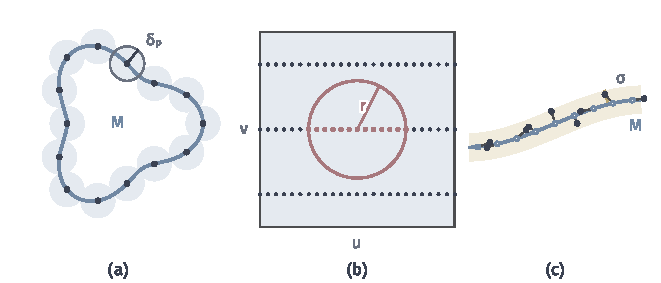
\includegraphics[width=112mm]{figures/04-spaces-measures-and-geometry/04-manifolds/matplotlib/mrec-coverage/figure.pdf}
  \caption{样本与流形的三种关系。(a) 曲线上$14$个样本（黑点），半径取覆盖精度$\delta_P$的圆盘把曲线盖满。(b) 一块平坦区域上的三条水平样本线，全域稠密，但红圈内的样本全在一条线上，只提供$u$方向的信息。(c) 观测（黑点）由真实采样点（空心点）沿任意方向偏移不超过$\sigma$，都落在曲线的$\sigma$管状邻域（浅黄）内。}
  \label{fig:mrec-coverage}
\end{BookInlineFigure}

\paragraph{局部邻域}

后面的局部计算都在某个位置附近进行。对选定的中心$\bm c\in\mathbb R^D$和半径$r>0$，记邻域样本为
\begin{equation}
 N_r(\bm c)=\{\bm p\in P:\lVert\bm p-\bm c\rVert_2\leq r\}.
 \label{eq:mrec-neighborhood}
\end{equation}
中心可以是一个样本，也可以是需要估计的任意位置。选邻域有定半径和定点数两种做法。本章采用定半径，因为$r$是一个明确的几何尺度，可以直接与覆盖精度和后面的可达半径比较；按点数选取时，各处的半径随采样疏密而变。

\paragraph{全域稠密与方向分布}

全域稠密只说明每一点附近都有样本，并不说明在某个邻域内，样本沿流形的各个方向都铺开了。设$M$的一块区域是平的，用坐标$(u,v)\in[0,1]^2$表示，例如平环面上的一小块。在这块区域上只沿三条水平线$v=\tfrac16,\tfrac12,\tfrac56$取样，每条线上的样本间距为$\tfrac1{24}$，如图~\ref{fig:mrec-coverage}(b)。

这组样本在全域上相当密。最孤立的点在两条水平线的正中间，又在两个相邻样本的正中间，所以
\[
 \delta_P=\sqrt{\bigl(\tfrac16\bigr)^2+\bigl(\tfrac1{48}\bigr)^2}\approx0.168 .
\]

现在以水平线上的一个样本为中心取半径$r=0.25$。相邻水平线的间隔是$\tfrac13>r$，所以邻域里的$13$个样本全在同一条水平线上。它们沿$u$方向铺开，完全不提供$v$方向的信息，后面的局部线性拟合会得到秩不足的矩阵。

所以全域稠密不能单独保证局部拟合的秩和条件数，邻域内的方向分布要另作要求。第~\ref{sec:mrec-tangent-error}节把这一要求写成局部矩阵的特征值条件。

\subsection{观测扰动}
\label{sec:mrec-noise}

实际观测很少恰好落在流形上。把第$i$个观测写成
\begin{equation}
 \bm x_i=\bm p_i+\bm e_i,\qquad\bm p_i\in M,\quad\lVert\bm e_i\rVert_2\leq\sigma ,
 \label{eq:mrec-noise-model}
\end{equation}
其中$\bm p_i$是看不到的真实采样位置，$\bm e_i$是环境空间中的有界扰动，方向任意，如图~\ref{fig:mrec-coverage}(c)。

这一模型把两种误差分开记录：真实采样点的覆盖精度$\delta_P$描述流形上有没有空缺，扰动界$\sigma$描述观测离开流形多远。由三角不等式，每个观测到$M$的距离不超过$\sigma$；而$M$上任一点先走到最近的真实采样点，再走到对应的观测，所以
\[
 \min_i\lVert\bm x-\bm x_i\rVert_2\leq\delta_P+\sigma,\qquad\bm x\in M.
\]

扰动改变了能够谈论的对象。$\bm x_i\notin M$时，$\bm x_i$处的切空间没有定义，$d_M(\bm x_i,\bm x_j)$也没有定义，能估计的只是附近真实位置处的量。所以无噪声的结论不能直接搬过来，每个结论都要重新说明$\sigma$进入哪里。

不同的任务对$\sigma$的要求也不同。邻域选择只受环境距离影响，每个成对距离至多变化$2\sigma$。局部拟合要求$\sigma$相对邻域半径小，才能把法向噪声与沿流形的展开区分开。拓扑恢复要求$\sigma$相对流形本身的尺度小，否则噪声可能填掉细小的孔洞。后面各节分别处理。

本章把扰动看成确定的有界量，只问“给定这些界，结论是否成立”。若样本按某个分布随机抽取、噪声是随机变量，则覆盖精度与扰动界都变成随机量，要估计它们以多大概率不超过给定值，可参考\BookChapterRef{chap:finite-sample-error-bounds}{卷八第4章“有限样本的误差上界”}。

\subsection{可达半径}
\label{sec:mrec-reach}

覆盖精度只说明样本多密，还缺一个描述流形自身形状的尺度：样本要密到什么程度，才算“相对于流形足够密”？直观上，流形弯得越厉害，或者它的不同部分靠得越近，所需的样本就越密。这两种情况可以用同一个量刻画。

对$\bm x\in\mathbb R^D$，记$\bm x$到$M$的距离为
\[
 \operatorname{dist}(\bm x,M)=\min_{\bm p\in M}\lVert\bm x-\bm p\rVert_2 .
\]
由$M$紧致，最小值可以取到，取到最小值的点称为$\bm x$在$M$上的最近点。$M$上的点的最近点是它自己；离开$M$以后，最近点可能不唯一，例如平面上单位圆的圆心到圆上每一点的距离都是$1$。

把$M$向外加粗，记
\[
 M^r=\{\bm x\in\mathbb R^D:\operatorname{dist}(\bm x,M)<r\}.
\]
可以想象从$M$出发同时向四面八方“长肉”，$M^r$是长到厚度$r$时的形状。厚度很小时，$M^r$里的每一点都能找回唯一的出发点；厚度增大，从不同地方长出来的部分迟早相撞，相撞处的点就有了两个最近点。可达半径就是这个相撞发生之前的最大厚度。

\begin{definition}[可达半径]
\label{def:mrec-reach}
$M$的\term{可达半径}（reach）定义为
\begin{equation}
 \tau=\sup\{r\geq0:M^r\text{中每一点在}M\text{上都有唯一最近点}\}.
 \label{eq:mrec-reach}
\end{equation}
\end{definition}

半径为$R$的圆的可达半径为$R$：圆心以外的每一点都有唯一最近点，即沿径向的那一点，而圆心离圆的距离恰为$R$。对紧致无边界的光滑嵌入子流形总有$\tau>0$，这是管状邻域定理的推论，证明可查阅Federer关于曲率测度的论文。

在$M^\tau$内，可以定义最近点投影$\pi$：$\pi(\bm x)$是$\bm x$在$M$上唯一的最近点。这个投影是连续的。设$\bm x_k\to\bm x$都在$M^\tau$中，由$M$紧致，$\pi(\bm x_k)$的任一收敛子列有极限$\bm z\in M$，并且
\[
 \lVert\bm x-\bm z\rVert_2=\lim_k\lVert\bm x_k-\pi(\bm x_k)\rVert_2=\lim_k\operatorname{dist}(\bm x_k,M)=\operatorname{dist}(\bm x,M).
\]
所以$\bm z$是$\bm x$的最近点，由唯一性$\bm z=\pi(\bm x)$。每个收敛子列的极限都是$\pi(\bm x)$，于是$\pi(\bm x_k)\to\pi(\bm x)$。

最近点还有一条一阶条件：$\bm x-\pi(\bm x)$与$M$在$\pi(\bm x)$处的切空间垂直。这是因为沿$M$上过$\pi(\bm x)$的任一曲线，到$\bm x$的距离平方在$\pi(\bm x)$处取最小值，导数为零。

\paragraph{限制可达半径的三种情形}

可达半径同时受三种因素限制，图~\ref{fig:mrec-reach-limits}分别画出了它们。

第一种是局部弯曲。图中是长半轴$2$、短半轴$1$的椭圆。在长轴端点$(2,0)$处曲率半径为$b^2/a=\tfrac12$，沿内法向走到曲率中心$(\tfrac32,0)$，这里是所有“最近点不唯一”的位置组成的线段的端点。一般地，曲线上曲率为$\kappa$的点使$\tau\leq1/\kappa$，圆的情形正是$\tau=R=1/\kappa$，椭圆的可达半径正是$\tfrac12$。

第二种是同一分支的不同部分相互接近。图~\ref{fig:mrec-reach-limits}(b)的闭曲线在中部收窄，两股相距$2b$，那里的曲率并不大，但中点$\bm z$到上下两股的距离相等，有两个最近点，所以$\tau\leq b$。第三种是不同分支相互接近，这时分支之间的距离直接控制可达半径。

\begin{BookInlineFigure}
  \centering
  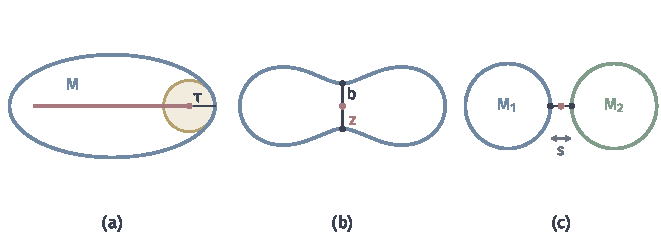
\includegraphics[width=112mm]{figures/04-spaces-measures-and-geometry/04-manifolds/matplotlib/mrec-reach-limits/figure.pdf}
  \caption{限制可达半径的三种情形。(a) 椭圆内部红色线段上的点都有两个或更多最近点，线段端点是长轴端点的曲率中心，到曲线的距离$\tau=\tfrac12$是这一位置的曲率半径。(b) 曲线中部收窄，中点$\bm{z}$有上下两个最近点，$\tau\leq b$。(c) 两个分支相距$s$，中点（红）同样有两个最近点，$\tau\leq s/2$。}
  \label{fig:mrec-reach-limits}
\end{BookInlineFigure}

\begin{lemma}[不同分支的间隔]
\label{lem:mrec-component-gap}
$M$的任意两个不同连通分支之间的环境距离不小于$2\tau$。
\end{lemma}
\begin{proof}
紧致流形只有有限个分支，每个分支紧致。所以在所有“属于不同分支”的点对中，环境距离的最小值$s$可以由某对$\bm p\in M_1$、$\bm q\in M_2$取到。

假设$s<2\tau$，取中点$\bm z=\tfrac12(\bm p+\bm q)$，则$\operatorname{dist}(\bm z,M)\leq s/2<\tau$，$\bm z$有唯一最近点$\bm w$。若$\lVert\bm z-\bm w\rVert_2=s/2$，则$\bm p,\bm q$都是$\bm z$的最近点，与唯一性矛盾，所以
\[
 \lVert\bm z-\bm w\rVert_2<\frac s2 .
\]

由三角不等式，
\[
 \lVert\bm p-\bm w\rVert_2\leq\lVert\bm p-\bm z\rVert_2+\lVert\bm z-\bm w\rVert_2<s,
\]
同样$\lVert\bm q-\bm w\rVert_2<s$。而$\bm w$所在的分支至少与$M_1$、$M_2$之一不同，这就找到了一对距离小于$s$的不同分支的点，与$s$的最小性矛盾。所以$s\geq2\tau$。
\end{proof}

\paragraph{可达半径控制的局部几何}

后面要用可达半径控制两件事：流形离切平面有多远，沿流形的路程比直线长多少。先看一个几何事实。在$\bm q\in M$处取单位法向量$\bm v$，沿它走一小段距离$s$，到达的点$\bm q+s\bm v$的最近点应当还是$\bm q$。下面的引理说，这一点一直保持到$s=\tau$。

\begin{lemma}[法向线段]
\label{lem:mrec-normal-segment}
设$\bm q\in M$，$\bm v$是$M$在$\bm q$处的单位法向量，$0\leq s<\tau$，则$\pi(\bm q+s\bm v)=\bm q$。
\end{lemma}
\begin{proof}
记$M$的法丛为
\[
 N=\{(\bm a,\bm w):\bm a\in M,\ \bm w\perp T_{\bm a}M\}.
\]
用局部的法向标准正交标架作坐标，可知$N$是$D$维流形。定义映射
\[
 \Phi:M^\tau\to N,\qquad\Phi(\bm x)=\bigl(\pi(\bm x),\ \bm x-\pi(\bm x)\bigr).
\]
由最近点的一阶条件，$\Phi$确实落在$N$中；由$\pi$连续，$\Phi$连续。

$\Phi$是单射，因为由$\Phi(\bm x)$相加两个分量就得到$\bm x$。$M^\tau$是$\mathbb R^D$的开集，$N$是$D$维流形，由Brouwer的区域不变性定理，连续单射$\Phi$的像$\Phi(M^\tau)$是$N$的开集。

令$A=\{s\in[0,\tau):\pi(\bm q+s\bm v)=\bm q\}$。首先$0\in A$。由$\pi$连续，$A$在$[0,\tau)$中是闭的。

再看$A$是开的。设$s\in A$，则
\[
 (\bm q,s\bm v)=\Phi(\bm q+s\bm v)\in\Phi(M^\tau).
\]
$\Phi(M^\tau)$是开集，所以当$s'$靠近$s$时$(\bm q,s'\bm v)$也在其中，即存在$\bm y\in M^\tau$使
\[
 \Phi(\bm y)=(\bm q,s'\bm v).
\]
相加两个分量得$\bm y=\bm q+s'\bm v$，并且$\pi(\bm y)=\bm q$，这就是$s'\in A$。

$[0,\tau)$连通，$A$既开又闭且非空，所以$A=[0,\tau)$。
\end{proof}

这条引理有一幅很直观的图像：在$\bm q$处沿法向放一个半径略小于$\tau$的球，球心是$\bm q+s\bm v$，引理说球内部不含$M$的点。可以想象一个半径为$\tau$的球沿$M$滚动，它能贴着$M$走遍每一点而不被挤开，如图~\ref{fig:mrec-rolling-ball}(a)。把这幅图写成不等式，就得到流形偏离切平面的界。

\begin{lemma}[法向偏离]
\label{lem:mrec-normal-distance}
对任意$\bm p,\bm q\in M$，$\bm q-\bm p$到切空间$T_{\bm p}M$的距离满足
\begin{equation}
 \operatorname{dist}(\bm q-\bm p,\ T_{\bm p}M)\leq\frac{\lVert\bm q-\bm p\rVert_2^2}{2\tau}.
 \label{eq:mrec-reach-normal}
\end{equation}
\end{lemma}
\begin{proof}
把$\bm q-\bm p$分解为切向部分与法向部分$\bm n$，式~\eqref{eq:mrec-reach-normal}的左端就是$\lVert\bm n\rVert_2$。$\bm n=\bm 0$时不用证，否则令$\bm v=\bm n/\lVert\bm n\rVert_2$。

对$0<s<\tau$，由引理~\ref{lem:mrec-normal-segment}，$\bm p$是$\bm p+s\bm v$的最近点，所以$\bm q$到它的距离不小于$s$：
\[
 \lVert\bm q-\bm p-s\bm v\rVert_2^2\geq s^2 .
\]
展开左端，并注意切向部分与$\bm v$垂直，$\bm q-\bm p$在$\bm v$上的分量就是$\lVert\bm n\rVert_2$，得
\[
 \lVert\bm q-\bm p\rVert_2^2-2s\lVert\bm n\rVert_2\geq0 .
\]
令$s\to\tau$，就得到式~\eqref{eq:mrec-reach-normal}。
\end{proof}

\begin{BookInlineFigure}
  \centering
  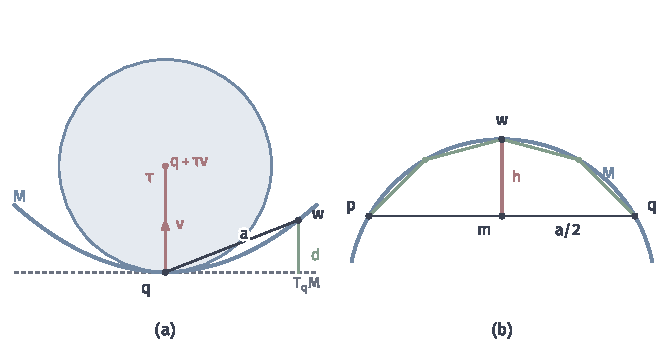
\includegraphics[width=112mm]{figures/04-spaces-measures-and-geometry/04-manifolds/matplotlib/mrec-rolling-ball/figure.pdf}
  \caption{可达半径的两个局部结论。(a) 半径为$\tau$的球（浅蓝）贴在$M$上，内部不含$M$的点，由此$\bm w$到切线的距离$d\leq a^2/(2\tau)$，其中$a$是$\bm q$到$\bm w$的弦长。(b) 半径为$\tau$的圆是引理~\ref{lem:mrec-midpoint}的极端情形：弦$\bm p\bm q$的中点$\bm m$投影到$\bm w$，两段新弦（绿）的长度恰为$2\tau\sin(\theta/2)$；继续细分，折线长度趋于弧长$2\tau\theta$。}
  \label{fig:mrec-rolling-ball}
\end{BookInlineFigure}

要控制沿流形的路程，办法是不断取弦的中点并投影回$M$，每投影一次，弦就更贴近流形，如图~\ref{fig:mrec-rolling-ball}(b)。下面的引理把一次投影的效果算清楚：它对中点的最近点用两次式~\eqref{eq:mrec-reach-normal}，把$\bm p$、$\bm q$到它的距离一起控制住。

\begin{lemma}[中点投影]
\label{lem:mrec-midpoint}
设$\bm p,\bm q\in M$，$a=\lVert\bm p-\bm q\rVert_2<2\tau$，把$a$写成$2\tau\sin\theta$，$\theta\in[0,\pi/2)$。则存在$\bm w\in M$，使
\begin{equation}
 \max\bigl(\lVert\bm p-\bm w\rVert_2,\ \lVert\bm q-\bm w\rVert_2\bigr)\leq2\tau\sin\frac\theta2 .
 \label{eq:mrec-midpoint}
\end{equation}
\end{lemma}
\begin{proof}
令$\bm m=\tfrac12(\bm p+\bm q)$，它到$\bm p$的距离是$a/2$，所以$\operatorname{dist}(\bm m,M)\leq a/2<\tau$，可取最近点$\bm w=\pi(\bm m)$，记$h=\lVert\bm m-\bm w\rVert_2$。

$h=0$时$\bm w=\bm m$，到两端的距离都是$a/2$，而
\[
 \frac a2=\tau\sin\theta\leq2\tau\sin\frac\theta2 ,
\]
结论成立。下设$h>0$。

令$\bm v=(\bm m-\bm w)/h$，由一阶条件，$\bm v$是$\bm w$处的单位法向量。记$c=\langle\bm p-\bm m,\bm v\rangle$，由对称性不妨设$c\geq0$，再记$A=a^2/4+h^2$。

按$\bm p-\bm w=(\bm p-\bm m)+(\bm m-\bm w)$展开，并用$\bm q-\bm m=-(\bm p-\bm m)$，得
\[
 \lVert\bm p-\bm w\rVert_2^2=A+2hc,\qquad\lVert\bm q-\bm w\rVert_2^2=A-2hc .
\]
同时，$\bm p-\bm w$在$\bm v$上的分量是$h+c$，$\bm q-\bm w$在$\bm v$上的分量是$h-c$。

对$\bm p$、$\bm w$与$\bm q$、$\bm w$分别用式~\eqref{eq:mrec-reach-normal}，得
\[
 h+c\leq\frac{A+2hc}{2\tau},\qquad h-c\leq\frac{A-2hc}{2\tau}.
\]
两式相加，得到
\[
 2\tau h\leq A,\qquad\text{即}\quad h^2-2\tau h+\frac{a^2}4\geq0 .
\]
又$h\leq a/2<\tau$，所以$h$不超过这个二次式的较小根：
\[
 h\leq h_*=\tau-\sqrt{\tau^2-a^2/4}=\tau(1-\cos\theta).
\]

从第一式解出$c$，由$\tau-h>0$，
\[
 c\leq\frac{A-2\tau h}{2(\tau-h)}.
\]
代回$\lVert\bm p-\bm w\rVert_2^2=A+2hc$，整理得
\[
 \lVert\bm p-\bm w\rVert_2^2\leq g(h)=\frac{\tau(a^2/4-h^2)}{\tau-h}.
\]

对$g$求导，
\[
 g'(h)=\frac{\tau(h^2-2\tau h+a^2/4)}{(\tau-h)^2}\geq0,\qquad 0\leq h\leq h_*,
\]
所以$g(h)\leq g(h_*)$。用$a/2=\tau\sin\theta$代入，
\[
 g(h_*)=\frac{\tau\cdot2\tau^2\cos\theta(1-\cos\theta)}{\tau\cos\theta}=2\tau^2(1-\cos\theta)=\bigl(2\tau\sin\tfrac\theta2\bigr)^2 .
\]
由$c\geq0$，$\bm q$到$\bm w$的距离不超过$\bm p$到$\bm w$的距离，所以两段距离都不超过$2\tau\sin(\theta/2)$。
\end{proof}

把式~\eqref{eq:mrec-reach-normal}和反复投影的结果写在一起，就是后面各节反复使用的两条局部推论。

\begin{theorem}[可达半径的局部推论]
\label{thm:mrec-reach-consequences}
设$M$的可达半径为$\tau>0$，$\bm p,\bm q\in M$。则$\bm q-\bm p$到$T_{\bm p}M$的距离满足式~\eqref{eq:mrec-reach-normal}。若$\lVert\bm p-\bm q\rVert_2<2\tau$，则$\bm p,\bm q$属于同一分支，并且
\begin{equation}
 d_M(\bm p,\bm q)\leq2\tau\arcsin\frac{\lVert\bm p-\bm q\rVert_2}{2\tau}.
 \label{eq:mrec-reach-arc}
\end{equation}
\end{theorem}

\begin{proof}
第一条就是引理~\ref{lem:mrec-normal-distance}。再看第二条，由引理~\ref{lem:mrec-component-gap}，$\bm p,\bm q$在同一分支。把$\lVert\bm p-\bm q\rVert_2$写成$2\tau\sin\theta$，$\theta<\pi/2$。对$\bm p,\bm q$用引理~\ref{lem:mrec-midpoint}得到$\bm w$，再对$(\bm p,\bm w)$和$(\bm w,\bm q)$分别用一次，如此重复$k$轮。

每轮把相邻两点弦长对应的角减半，$k$轮后得到$M$上$2^k+1$个点，相邻点的距离都不超过$2\tau\sin(\theta/2^k)$，这些弦长的总和不超过
\[
 2^k\cdot2\tau\sin\frac\theta{2^k}\leq2\tau\theta .
\]
在紧致流形上，$\lVert\bm x-\bm y\rVert_2\to0$时$d_M(\bm x,\bm y)/\lVert\bm x-\bm y\rVert_2$一致趋于$1$，因为$M$在小尺度上是斜率很小的图。所以对任意$\eta>0$，$k$足够大时
\[
 d_M(\bm p,\bm q)\leq(1+\eta)\,2\tau\theta .
\]
令$\eta\to0$，并由$\theta=\arcsin(\lVert\bm p-\bm q\rVert_2/2\tau)$，得式~\eqref{eq:mrec-reach-arc}。
\end{proof}

两条结论在圆上都取等号。在半径为$R$的圆上，取$\bm p$处的切线为水平方向，$\bm q$对应圆心角$\theta$，则法向分量为$R(1-\cos\theta)$，弦长的平方为$2R^2(1-\cos\theta)$，式~\eqref{eq:mrec-reach-normal}取等号；弦长$s$对应的弧长为$2R\arcsin(s/2R)$，式~\eqref{eq:mrec-reach-arc}也取等号。所以这两个估计不能再改进。

第一条说，在半径为$r$的邻域内，流形偏离切平面至多$r^2/(2\tau)$，相对于邻域半径的比值是$r/(2\tau)$。第二条说，环境距离小于$2\tau$的两点，沿流形的距离不会比直线长太多：$\lVert\bm p-\bm q\rVert_2\leq\tau$时，比值至多为$2\arcsin\tfrac12=\pi/3\approx1.047$。

第一条还给出弯曲的上界。设$\gamma$是$M$上过$\bm p$的单位速度测地线，$\gamma(s)-\bm p$的切向部分近似$s\gamma'(0)$，法向部分近似$\tfrac12s^2\gamma''(0)$，而弦长近似$s$。代入式~\eqref{eq:mrec-reach-normal}，令$s\to0$，得$\lVert\gamma''(0)\rVert_2\leq1/\tau$，即每条测地线作为$\mathbb R^D$中的曲线，曲率都不超过$1/\tau$。

\subsection{邻域尺度}
\label{sec:mrec-neighborhood-scale}

局部计算的成败，关键在邻域半径$r$的选取。图~\ref{fig:mrec-scale}用同一组带噪声的样本比较了三种半径。

$r$过小时，邻域内的样本太少，甚至只有中心自己。即使样本不少，若$r$与扰动界$\sigma$同量级，邻域内样本的散布主要来自噪声，看不出流形的方向，如图(a)。所以$r$要明显大于覆盖精度$\delta_P$和$\sigma$。

$r$过大时出现另外两类问题。由定理~\ref{thm:mrec-reach-consequences}，流形在邻域内偏离切平面可达$r^2/(2\tau)$，$r$与$\tau$可比时这一偏离与邻域本身一样大，局部已不能看成平的。另外，$r$超过两股的间隔时，邻域会同时包含两股的样本，如图(c)，它们在环境中靠近，沿流形却相距很远。

由定理~\ref{thm:mrec-reach-consequences}的第二条，$r<2\tau$时邻域内的点都属于同一分支；要使局部线性近似可靠，还要$r$远小于$\tau$。所以分析的范围大致是
\begin{equation}
 \delta_P,\ \sigma\ll r\ll\tau .
 \label{eq:mrec-scale-range}
\end{equation}

\begin{BookInlineFigure}
  \centering
  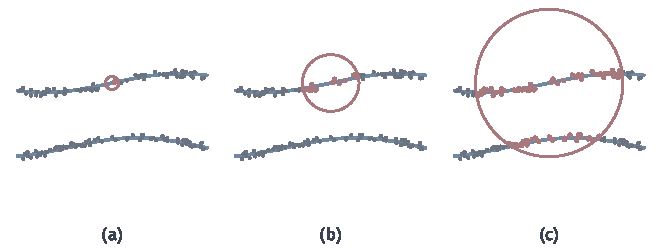
\includegraphics[width=112mm]{figures/04-spaces-measures-and-geometry/04-manifolds/matplotlib/mrec-scale/figure.pdf}
  \caption{同一组带噪声的样本在三种邻域半径下的情形，两条蓝线是流形的两股，红点是邻域内的样本。(a) 半径与噪声同量级，邻域内只有零星几个点。(b) 半径适中，邻域内的样本沿一股展开。(c) 半径超过两股的间隔，邻域混入另一股的样本。}
  \label{fig:mrec-scale}
\end{BookInlineFigure}

\paragraph{嵌入弯曲决定局部线性误差}

第~\ref{chap:riemannian-geometry}章区分了内在曲率与嵌入弯曲。半径为$\rho$的圆柱面内在地是平的，可以展开成平面而不改变任何长度，如图~\ref{fig:mrec-cylinder}(b)；但它在$\mathbb R^3$中弯曲，可达半径为$\rho$，切平面只在一条母线上贴着它，如图~\ref{fig:mrec-cylinder}(a)。

取$\rho=1$，沿圆周方向取一点，弦长$r=0.5$，它对应的圆心角$\theta$满足$2\sin(\theta/2)=0.5$，到切平面的距离是
\[
 1-\cos\theta=\frac{r^2}{2\rho}=0.125 .
\]
内在曲率为零并没有让这一偏离消失；沿母线方向偏离却恰好是零。这说明局部线性误差首先由环境中的嵌入形状决定，可达半径度量的正是这一形状，内在曲率是另一回事。

\begin{BookInlineFigure}
  \centering
  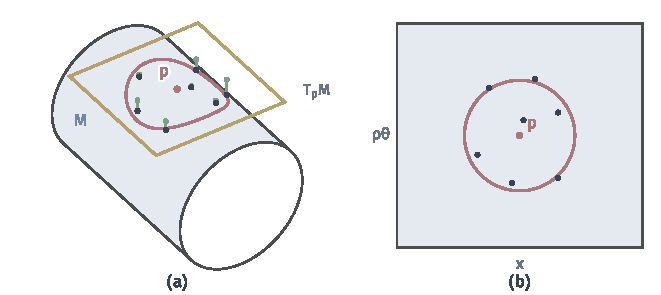
\includegraphics[width=112mm]{figures/04-spaces-measures-and-geometry/04-manifolds/matplotlib/mrec-cylinder/figure.pdf}
  \caption{圆柱面的内在几何与嵌入形状。(a) 点$\bm{p}$处的切平面（黄色框）与红圈内的邻域，绿色线段是样本（黑点）到切平面的法向偏离，沿圆周方向偏离最大。(b) 把圆柱面沿母线剪开摊平，同一邻域和样本成为平面上的圆盘和点，长度不变，内在曲率为零。}
  \label{fig:mrec-cylinder}
\end{BookInlineFigure}

反过来，即使嵌入弯曲很小，邻域内样本的方向覆盖仍需单独核验，第~\ref{sec:mrec-coverage}节的水平线采样就是例子。选定$r$以后，邻域应同时满足三条：足够小，使弯曲可以忽略；足够大，使样本数和散布压过噪声；样本在各个切向上都有展开。

\section{切空间估计}
\label{sec:mrec-tangent}

切空间是流形在一点处的线性近似。第~\ref{chap:manifold-basics}章用曲线的速度或局部坐标定义它，第~\ref{chap:manifold-relations}章说明嵌入子流形的切空间是环境空间的线性子空间。现在只有样本，没有局部坐标，也没有曲线。

本节先说明切空间在什么意义上近似流形，再把这一近似落实为有限样本上的子空间拟合，最后分析拟合误差。局部主成分分析是一种估计方法，它的输出只有在几何近似成立时才是切空间的近似，不能反过来把它当作切空间的定义。

\subsection{切向近似}
\label{sec:mrec-tangent-approx}

在点$\bm p\in M$附近，把环境空间分解为切空间$T=T_{\bm p}M$与它的正交补，即法空间$T^\perp$。把$M$上的点正交投影到$T$，这个映射在$\bm p$处的导数是$T$上的恒等映射，由反函数定理在局部可逆。

它的逆就给出参数化$\bm u\mapsto\bm p+\bm u+g(\bm u)$。也就是说，存在$\bm0$在$T$中的邻域$W$和$C^2$映射$g:W\to T^\perp$，使$M$在$\bm p$附近的部分恰为
\begin{equation}
 \{\bm p+\bm u+g(\bm u):\bm u\in W\},\qquad g(\bm0)=\bm0,\quad Dg(\bm0)=\bm0 .
 \label{eq:mrec-local-graph}
\end{equation}
这里的$g$就是图~\ref{fig:mrec-cylinder}(a)中那些绿色线段的长度和方向：从切平面上的$\bm u$沿法向走$g(\bm u)$，就回到流形。

条件$Dg(\bm0)=\bm0$表达的正是切空间的局部线性作用：沿切向移动$\bm u$，流形在法向上的偏离没有一阶项。对$C^2$的$g$，若它的二阶导数在$W$中某个凸邻域上的范数不超过$K$，由多元Taylor公式，在这个邻域中
\[
 \lVert g(\bm u)\rVert_2\leq\frac K2\lVert\bm u\rVert_2^2 .
\]
多元Taylor展开与余项可参考\BookChapterRef{chap:multivariate-differentiation}{卷二第17章“多元函数微分”}。这个界依赖图函数的坐标，式~\eqref{eq:mrec-reach-normal}给出不依赖坐标的同类界，只用到可达半径。

这是邻域尺度下的近似，不是全局平面表示。以半径为$R$的圆为例，在最低点处取水平切线，图函数是
\[
 g(u)=R-\sqrt{R^2-u^2}=\frac{u^2}{2R}+O(u^4),
\]
二次项正是曲率决定的偏离。但这个表示只在$\lvert u\rvert<R$时有定义，越过左右两端，圆就不再是水平线上的图，切线近似也随之失去意义。

\subsection{局部PCA}
\label{sec:mrec-local-pca}

切向近似说明，在小邻域内，流形上的点主要沿切向展开，法向偏离是二阶小量。于是可以把邻域内的样本当作一团数据，寻找它们展开最多的$m$个方向。这里假定流形的维数$m$已经指定，邻域也已选定，记其中的观测为$\bm x_1,\ldots,\bm x_k$。

\paragraph{局部协方差与主方向}

计算局部质心与局部协方差矩阵
\begin{equation}
 \overline{\bm x}=\frac1k\sum_{j=1}^k\bm x_j,\qquad
 \bm C=\frac1k\sum_{j=1}^k(\bm x_j-\overline{\bm x})(\bm x_j-\overline{\bm x})^\top .
 \label{eq:mrec-local-covariance}
\end{equation}
$\bm C$是$D$阶对称半正定矩阵。取它最大的$m$个特征值对应的标准正交特征向量，排成$\widehat{\bm U}\in\mathbb R^{D\times m}$，其列空间$\widehat S$就是切空间的估计。这一方法称为\term{局部主成分分析}（local principal component analysis）。

主方向的意义来自一个最优性：$\widehat S$在全部$m$维线性子空间中，使中心化样本到子空间的平方距离和最小。记$\bm y_j=\bm x_j-\overline{\bm x}$，取$S$的一组标准正交基排成$\bm V\in\mathbb R^{D\times m}$。$\bm y_j$到$S$的距离的平方，是它的长度平方减去投影长度的平方，所以
\[
 \begin{aligned}
 \sum_j\operatorname{dist}(\bm y_j,S)^2
 &=\sum_j\lVert\bm y_j\rVert_2^2-\sum_j\lVert\bm V^\top\bm y_j\rVert_2^2\\
 &=k\operatorname{tr}\bm C-k\operatorname{tr}(\bm V^\top\bm C\bm V).
 \end{aligned}
\]
第一项与$S$无关，所以最小化距离和等价于最大化$\operatorname{tr}(\bm V^\top\bm C\bm V)$。它的最大值是前$m$个特征值之和，由前$m$个特征向量取到，这一迹极值可参考\BookChapterRef{chap:matrix-approximation}{卷二第15章“矩阵逼近”}。在全部$m$维仿射平面中，到样本的平方距离和最小的是$\overline{\bm x}+\widehat S$。

\paragraph{子空间、基与平面}

这里有三个不同的对象。$\widehat S$是方向子空间，是对$T_{\bm p}M$的估计。$\widehat{\bm U}$只是它的一组标准正交基，右乘任何$m$阶正交矩阵仍是同一个子空间的基，所以比较估计与真值时只能比较子空间，例如用主夹角。$\overline{\bm x}+\widehat S$是拟合平面，它还带有位置信息，而局部质心一般不在流形上，也不等于$\bm p$。

\paragraph{矩阵的秩不是流形的维数}

有限样本的协方差矩阵的秩不能直接当作真实维数。带噪声时$\bm C$一般满秩，秩等于$\min(D,k-1)$，与$m$无关；无噪声时，流形的弯曲也使样本不落在任何$m$维平面上，$\bm C$的秩仍可能大于$m$。

例~\ref{ex:mrec-one-sided}的三个点在一条曲线上，$m=1$，却算出秩为$2$的$\bm C$，两个特征值约为$4.43\times10^{-2}$和$2.0\times10^{-4}$。谱中前$m$个特征值明显大于其余，可以作为维数的线索，但要把它当作判断，就必须结合下一小节的误差分析说明“明显”的界限。本节始终把$m$看作已知。

\subsection{切空间估计的误差}
\label{sec:mrec-tangent-error}

现在估计$\widehat S$偏离$T=T_{\bm p}M$多远。误差有三个来源：流形在邻域内的弯曲，邻域内样本在切向上的分布，以及观测扰动。下面把它们分别写进局部协方差矩阵，再用特征子空间的扰动界控制方向的偏离。

所用的工具是\BookChapterRef{chap:condition-and-spectral-perturbation}{卷二第7章“条件数与谱扰动”}中的Davis--Kahan谱隙界。设对称矩阵$\bm C_0$扰动为$\bm C=\bm C_0+\bm E$，$\gamma=\lambda_m(\bm C_0)-\lambda_{m+1}(\bm C)>0$，则两者的前$m$个特征子空间的最大主夹角$\theta_{\max}$满足
\begin{equation}
 \sin\theta_{\max}\leq\frac{\lVert\bm E\rVert_2}{\gamma}.
 \label{eq:mrec-davis-kahan}
\end{equation}

\paragraph{误差的分解}

设邻域中观测$\bm x_j$对应的真实采样点$\bm p_j$满足$\lVert\bm p_j-\bm p\rVert_2\leq r$。把$\bm p_j-\bm p$分解为切向部分$\bm u_j\in T$与法向部分$\bm n_j\in T^\perp$，在图表示成立的范围内$\bm n_j=g(\bm u_j)$，于是
\[
 \bm x_j=\bm p+\bm u_j+\bm n_j+\bm e_j,\qquad\lVert\bm e_j\rVert_2\leq\sigma .
\]

用上划线表示邻域平均，记
\[
 \bm a_j=\bm u_j-\overline{\bm u}\in T,\qquad
 \bm b_j=(\bm n_j-\overline{\bm n})+(\bm e_j-\overline{\bm e}).
\]
则$\bm x_j-\overline{\bm x}=\bm a_j+\bm b_j$，切向展开全部在$\bm a_j$里，弯曲和噪声全部在$\bm b_j$里。代入式~\eqref{eq:mrec-local-covariance}，
\[
 \bm C=\bm C_0+\bm E,\qquad\bm C_0=\frac1k\sum_j\bm a_j\bm a_j^\top ,
\]
\[
 \bm E=\frac1k\sum_j\bigl(\bm a_j\bm b_j^\top+\bm b_j\bm a_j^\top+\bm b_j\bm b_j^\top\bigr).
\]

$\bm C_0$的像在$T$中，在$T^\perp$上为零。记它在$T$上的最小特征值为$\lambda_T$，它度量样本在最不充分的那个切向上展开了多少，第~\ref{sec:mrec-coverage}节的水平线采样中$\lambda_T=0$。

为了估计$\bm E$，先注意对任意向量组，
\[
 \Bigl\lVert\frac1k\sum_j\bm v_j\bm w_j^\top\Bigr\rVert_2\leq\max_j\lVert\bm v_j\rVert_2\max_j\lVert\bm w_j\rVert_2 .
\]
这是因为对单位向量$\bm y,\bm z$，由Cauchy不等式，$\bm y^\top\bm v_j$与$\bm w_j^\top\bm z$的绝对值分别不超过$\lVert\bm v_j\rVert_2$和$\lVert\bm w_j\rVert_2$，它们的乘积取平均不会变大。

再看两类向量的长度。由$\lVert\bm u_j\rVert_2\leq r$，得$\lVert\bm a_j\rVert_2\leq2r$。由式~\eqref{eq:mrec-reach-normal}，$\lVert\bm n_j\rVert_2\leq r^2/(2\tau)$，所以$\bm b_j$的长度不超过
\begin{equation}
 \beta=\frac{r^2}\tau+2\sigma .
 \label{eq:mrec-beta}
\end{equation}

\begin{theorem}[局部PCA的方向误差]
\label{thm:mrec-local-pca-error}
在上述假设下，$\lVert\bm E\rVert_2\leq4r\beta+\beta^2$，其中$\beta$由式~\eqref{eq:mrec-beta}给出。若$\lambda_T>0$且$4r\beta+\beta^2\leq\lambda_T/2$，则估计子空间$\widehat S$与$T_{\bm p}M$的最大主夹角满足
\begin{equation}
 \sin\theta_{\max}\leq\frac{2(4r\beta+\beta^2)}{\lambda_T}.
 \label{eq:mrec-local-pca-error}
\end{equation}
\end{theorem}
\begin{proof}
由前面的不等式，$\bm E$的三部分分别不超过$2r\beta$、$2r\beta$和$\beta^2$，所以$\lVert\bm E\rVert_2\leq4r\beta+\beta^2$。

$\bm C_0$的前$m$个特征值不小于$\lambda_T$，其余为零，前$m$个特征子空间就是$T$。由Weyl不等式，$\bm C$的第$m+1$个特征值不超过$\lVert\bm E\rVert_2$，于是
\[
 \gamma\geq\lambda_T-\lVert\bm E\rVert_2\geq\frac{\lambda_T}2 .
\]
代入式~\eqref{eq:mrec-davis-kahan}，即得式~\eqref{eq:mrec-local-pca-error}。
\end{proof}

\paragraph{方向覆盖与尺度的权衡}

分母$\lambda_T$要求样本在每个切向上都有展开，这正是第~\ref{sec:mrec-coverage}节所说的方向分布条件。若邻域内的样本在切向上铺得比较均匀，$\lambda_T$与$r^2$同量级，例如在$m$维圆盘上均匀分布时为$r^2/(m+2)$。设$\lambda_T\geq c\,r^2$，忽略高阶项，界的主要部分为
\begin{equation}
 \sin\theta_{\max}\lesssim\frac8c\Bigl(\frac r\tau+\frac{2\sigma}r\Bigr).
 \label{eq:mrec-pca-tradeoff}
\end{equation}
第一项来自弯曲，随$r$增大；第二项来自扰动，随$r$增大而减小。

所以缩小邻域并不总是更好。无噪声时取小的$r$可以压低弯曲误差，但$r$不能小到邻域内样本不足以在各切向上铺开，这要求$r$明显大于覆盖精度。有噪声时两项在$r$约为$\sqrt{2\sigma\tau}$处平衡，再小反而更差。图~\ref{fig:mrec-pca}(c)对单位圆上的单侧邻域算出了实际的方向误差，它在两条虚线相交的量级上取到最小值，曲线形状与式~\eqref{eq:mrec-pca-tradeoff}一致。

这个界是最坏情形的估计，常数偏大。取下面例子中的$c=\tfrac16$，要使定理的条件$4r\beta+\beta^2\leq\lambda_T/2$成立，无噪声时大约要$r\leq\tau/48$。定理的价值在于说明误差怎样依赖$r$、$\tau$、$\sigma$和$\lambda_T$，而不是给出紧的数值。

\begin{example}[单侧邻域的倾斜]
\label{ex:mrec-one-sided}
在抛物线$y=u^2/(2R)$上取$\bm p=(0,0)$，它在原点附近近似半径为$R$的圆，切线为横轴。

若邻域样本对称地取在$u=-h,0,h$处，由对称性，横向与纵向的协方差为零，主方向恰为横轴，横向方差$2h^2/3$远大于纵向方差$h^4/(18R^2)$。

若只取单侧的$u=0,h,2h$，三点的纵坐标是$0,\ h^2/(2R),\ 2h^2/R$，横向均值$\overline u=h$，纵向均值$\overline y=5h^2/(6R)$。逐项计算协方差矩阵的元素，得到
\[
 C_{uu}=\frac{2h^2}3,\qquad C_{uy}=\frac{2h^3}{3R},\qquad C_{yy}=\frac{13h^4}{18R^2}.
\]

主方向与横轴的夹角$\varphi$满足
\[
 \tan2\varphi=\frac{2C_{uy}}{C_{uu}-C_{yy}}\approx\frac{2h}R,
\]
所以$\varphi\approx h/R$。这恰好是抛物线在质心横坐标$u=h$处的切线斜率：估计出的其实是质心附近的切方向，相对于$T_{\bm p}M$的偏离是$r/\tau$量级，与定理中的弯曲项一致。

取$R=1$，$h=0.25$代入，$C_{uu}\approx0.0417$，$C_{uy}\approx0.0104$，$C_{yy}\approx0.0028$，于是$\tan2\varphi\approx0.536$，$\varphi\approx14.1^\circ$，而$\arctan(h/R)\approx14.0^\circ$。
\end{example}

图~\ref{fig:mrec-pca}(a)(b)画出了这两种邻域。对称邻域把弯曲的影响抵消了，单侧邻域则把主方向带向质心处的切线，这一倾斜不会因为增加样本而消失。

\begin{BookInlineFigure}
  \centering
  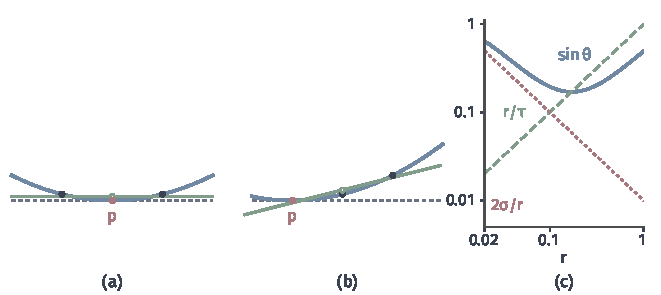
\includegraphics[width=112mm]{figures/04-spaces-measures-and-geometry/04-manifolds/matplotlib/mrec-pca/figure.pdf}
  \caption{局部PCA的方向误差。(a)(b) 抛物线$y=u^2/2$上$h=0.25$的对称与单侧邻域，黑点是样本，空心点是局部质心，绿线是主方向，虚线是$\bm{p}$处的真实切线；单侧时主方向倾斜$14.1^\circ$。(c) 单位圆上单侧弧$[0,r]$内$41$个样本加法向扰动$\sigma=0.005$时的实际误差（蓝），与弯曲项$r/\tau$（绿）、扰动项$2\sigma/r$（红）的比较，纵轴和横轴都取对数。}
  \label{fig:mrec-pca}
\end{BookInlineFigure}

\section{局部流形拟合}
\label{sec:mrec-local-fit}

切空间估计只给出一个平面，而流形在邻域内是弯的。要得到穿过或逼近样本的连续曲面片，还需要描述法向上怎样随切向坐标变化。本节在估计的平面上建立局部坐标，把法向分量拟合成切向坐标的函数，再分析拟合片的误差以及多片能否拼起来。拟合目标的加权、正则化等更一般的选择，以及相应的数值优化，属于\BookChapterRef{chap:optimization}{卷五第1章“优化问题与解”}开始的优化理论，本节只用普通最小二乘。

\subsection{局部图函数的拟合}
\label{sec:mrec-graph-fit}

设已选定局部中心$\bm q\in\mathbb R^D$，例如一个样本或局部质心，以及估计子空间的标准正交基$\widehat{\bm U}\in\mathbb R^{D\times m}$。把它补成$\mathbb R^D$的标准正交基$[\widehat{\bm U},\widehat{\bm V}]$，对邻域内每个观测计算切向坐标与法向分量
\[
 \bm u_j=\widehat{\bm U}^\top(\bm x_j-\bm q)\in\mathbb R^m,\qquad
 \bm w_j=\widehat{\bm V}^\top(\bm x_j-\bm q)\in\mathbb R^{D-m}.
\]
目标是找函数$g$使$\bm w_j\approx g(\bm u_j)$，由此得到连续片
\begin{equation}
 \bm\phi(\bm u)=\bm q+\widehat{\bm U}\bm u+\widehat{\bm V}g(\bm u),\qquad\bm u\in\Omega ,
 \label{eq:mrec-patch}
\end{equation}
其中$\Omega\subseteq\mathbb R^m$是切向坐标的定义域，例如半径为$\rho$的球。

\paragraph{图表示的前提}

只有当流形在这个邻域内确实是估计平面上的图时，拟合才有意义。把$M$上的点投影到估计平面，这个映射在$\bm p$处的导数是从$T_{\bm p}M$到$\widehat S$的正交投影，它的奇异值是两个子空间主夹角的余弦。只要最大主夹角小于$\pi/2$，导数就可逆，由反函数定理，$M$在$\bm p$附近可以写成$\bm q+\widehat{\bm U}\bm u+\widehat{\bm V}\widetilde g(\bm u)$，$\widetilde g$是$C^2$的。夹角越小、邻域越小，这个图表示的定义域越大、$\widetilde g$越平缓。

\paragraph{为什么要保留常数项和一次项}

真实切空间上的图函数满足$g(\bm0)=\bm0$与$Dg(\bm0)=\bm0$，但估计平面上的$\widetilde g$一般不满足：$\bm q$未必在$M$上，所以$\widetilde g(\bm0)\neq\bm0$；估计平面有倾斜，所以$D\widetilde g(\bm0)\neq\bm0$。在例~\ref{ex:mrec-one-sided}中，估计方向的斜率约为$h/R$，抛物线在新坐标下于$\bm p$处的斜率约为$-h/R$。若强行要求一次项为零，邻域边缘$|u|\approx2h$处的拟合误差就有$2h^2/R$量级，与弯曲本身一样大。

所以把估计平面的偏差纳入模型，用含常数项、一次项和二次项的多项式拟合每个法向分量：
\[
 g(\bm u)=\bm c_0+\bm L\bm u+\bigl(\tfrac12\bm u^\top\bm Q_l\bm u\bigr)_{l=1}^{D-m},
\]
其中$\bm c_0\in\mathbb R^{D-m}$，$\bm L\in\mathbb R^{(D-m)\times m}$，每个$\bm Q_l$是$m$阶对称矩阵。每个法向分量有$1+m+m(m+1)/2$个系数，$m=1$时为$3$个，$m=2$时为$6$个。

\paragraph{系数的求解与约束}

系数关于数据是线性的。把每个$\bm u_j$处全部单项式的值排成一行，得到设计矩阵$\bm\Phi\in\mathbb R^{k\times N_c}$，$N_c=1+m+m(m+1)/2$；每个法向分量的系数是以$\bm\Phi$为设计矩阵的普通最小二乘解，其构造与核对可参考\BookChapterRef{chap:linear-solution-selection}{卷二第9章“线性方程与最小二乘的选解”}。系数唯一当且仅当$\bm\Phi$满列秩。

$\bm\Phi$满列秩有直接的几何含义：$\bm\Phi\bm a=\bm0$意味着系数为$\bm a$的二次多项式在全部$\bm u_j$处为零，所以$\bm\Phi$满列秩当且仅当没有非零的二次多项式在全部切向坐标处同时为零。$m=1$时，这要求至少有三个不同的$u_j$；$m=2$时，要求至少六个点且它们不全落在同一条二次曲线上，例如全部落在一条直线上就不行。这正是第~\ref{sec:mrec-coverage}节方向分布条件在二阶拟合中的形式。

\begin{example}[圆弧上的二次拟合]
\label{ex:mrec-circle-fit}
在半径为$R$的圆的最低点取$\bm q=\bm p=(0,0)$，切线为横轴，样本取在横坐标$u=-h,0,h$处，纵坐标为$w=c,0,c$，$c=R-\sqrt{R^2-h^2}$。三点恰好确定二次多项式，解得$g(u)=(c/h^2)u^2$，常数项与一次项为零，这是对称性的结果。

二次系数$c/h^2=1/(R+\sqrt{R^2-h^2})$，当$h\to0$时趋于$1/(2R)$，与真实图函数$R-\sqrt{R^2-u^2}=u^2/(2R)+u^4/(8R^3)+\cdots$的二次项一致。在样本处拟合与真值相等，在其他位置的差别来自四次项，$|u|\leq h$时为$h^4/R^3$量级。
\end{example}

\subsection{局部片的误差与拼接}
\label{sec:mrec-patch-error}

拟合片要与真实流形比较，就要在同一个定义域上比较同一种量。在估计平面的坐标域$\Omega$上，真实流形写成$\widetilde g$，拟合片写成$g$，法向偏差是$\sup_{\bm u\in\Omega}\lVert g(\bm u)-\widetilde g(\bm u)\rVert_2$。这个量把以下几种误差合在了一起，分析时要分别检查。

\paragraph{误差的来源}

第一是切空间估计的偏差。它本身不是拟合误差，而是改变了$\widetilde g$的形状：倾斜越大，$\widetilde g$的一次项越大、图表示的定义域越小，夹角接近$\pi/2$时图表示不复存在。模型含一次项可以吸收小的倾斜，但不能挽救大的倾斜。

第二是函数截断。$\widetilde g$一般不是二次多项式。若它是$C^3$的，在半径为$\rho$的定义域上，二次Taylor多项式的余项为$\rho^3$量级；若只知道它是$C^2$的，则只能说余项比$\rho^2$小，没有确定的阶。截断误差指$\widetilde g$中任何二次多项式都消除不了的部分，Taylor余项给出它的一个上界；最小二乘所得的多项式不一定就是Taylor多项式，但它也不可能比最好的二次多项式更接近$\widetilde g$。

第三是样本分布与观测噪声。设法向数据是$\widetilde g(\bm u_j)$加上偏差$\bm\eta_j$，偏差中既有截断余项，也有观测扰动。最小二乘系数的误差不超过$\lVert\bm\eta\rVert_2/\sigma_{\min}(\bm\Phi)$，其中$\sigma_{\min}(\bm\Phi)$是设计矩阵的最小奇异值；切向坐标挤在一起或接近落在同一条二次曲线上时，$\sigma_{\min}$小，偏差被放大。有界扰动可以有系统的方向，增加样本数并不自动使它平均掉。

\paragraph{函数值误差不控制导数}

法向偏差小，不说明拟合片的切方向或曲率也准确。设真实流形在局部是$w=0$的直线，观测沿$u$方向以间距$s$交替带有$+\sigma$与$-\sigma$的法向扰动。若用插值样本的折线作拟合片，每一点的函数值误差不超过$\sigma$，斜率却到处是$\pm2\sigma/s$；$s$越小，即样本越密，斜率误差反而越大。

固定阶数的多项式不会这样振荡，但它与$\widetilde g$之差一般不是多项式，函数值上的误差界不能直接换成导数上的误差界。要从拟合片读出切方向或曲率，需要对导数单独分析误差，函数值逼近只是其中一个条件。

\paragraph{多片的并不自动是流形}

在每个样本附近各拟合一片以后，所有片的并未必是光滑流形。相邻两片在重叠区域可能不一致，留下台阶或缝隙；来自两个相近分支的片可能彼此穿过，并集出现自交，在交线附近根本不是流形。要拼成一个整体，至少需要相邻片的坐标域相互重叠、在重叠处的坐标转换光滑且一致，并用适当的方式把各片平滑地合成一张曲面。

即使拼接成功，所得曲面与真实流形同胚，也需要额外的条件和论证，这已超出本节的范围。后面的同调恢复不以局部拟合为前提：第~\ref{sec:mrec-homology-recovery}节直接由样本的球并与复形得到拓扑信息，不需要先构造曲面。

\section{内在距离逼近}
\label{sec:mrec-intrinsic-distance}

沿流形从一点走到另一点有多远，即内在距离$d_M$，不能由两点的环境距离读出：螺旋卷起的纸面上，相邻两层的点环境距离很小，沿纸面却要绕很远。但在很小的尺度上，环境距离与内在距离几乎相同。于是可以用短边连接相邻的样本，再沿图上的路径把短距离一段段累加起来，逼近远处两点之间的内在距离。本节只在同一连通分支内比较，不同分支之间的内在距离为无穷，图上相应的距离也应为无穷。

\subsection{邻接图的构造}
\label{sec:mrec-neighborhood-graph}

先讨论按固定半径连边的图，它对应一个明确的几何尺度。

\begin{definition}[半径邻域图与图距离]
\label{def:mrec-neighborhood-graph}
给定样本$P=\{\bm p_1,\ldots,\bm p_n\}$和半径$r>0$，\term{邻域图}（neighborhood graph）$\mathcal G_r$以样本为顶点，$\lVert\bm p_i-\bm p_j\rVert_2\leq r$时连边$\{i,j\}$，边权为$\lVert\bm p_i-\bm p_j\rVert_2$。顶点$i,j$之间的\term{图距离}（graph distance）$d_{\mathcal G}(i,j)$是连接它们的路径的边权和的最小值，没有路径时为$+\infty$。
\end{definition}

图距离可以用最短路算法计算，边权非负时Dijkstra算法适用，可参考\BookChapterRef{chap:shortest-paths}{卷三第3章“最短路”}。这里的输入只有样本之间的环境距离，与直接使用流形上的测地距离不同：边权是弦长，不是弧长，并且只有不超过$r$的弦才被使用。每条边的弦长都不超过两端点的内在距离，这是低估的来源；路径只能经过样本，不能走真实的最短曲线，这是高估的来源。下一小节说明两者怎样平衡。

\paragraph{其他连边规则}

另一种常用规则是近邻图：每个样本连向离它最近的$k$个样本。这个关系不对称，$\bm p_j$是$\bm p_i$的近邻，$\bm p_i$未必是$\bm p_j$的近邻，需要声明用“或”还是用“且”把它对称化。更重要的是，固定$k$并不固定几何尺度：稀疏处第$k$个近邻可能很远，稠密处则很近。

所以近邻图要按它实际产生的边来核对条件：最长的边是否小于可达半径给出的界，最短的那些边是否足以跨过采样的空隙。下面的结论只依赖“所有边都不超过某个长度”与“所有足够短的点对都连了边”这两条性质，对近邻图需要分别验证。

\paragraph{连通不等于可靠}

图是否连通与图距离是否可靠是两回事。一条错误地连接了两个远处部分的边，会使图更加连通，同时让大量点对的图距离严重偏小。反过来，图不连通时，同一分支内的点对会得到无穷的图距离，这也是错的。连通性只是一个必要的检查，不能代替下面的误差分析。

\subsection{图距离的误差}
\label{sec:mrec-graph-distance-error}

下面假定样本在$M$上、无噪声，用覆盖精度$\delta$与可达半径$\tau$控制图距离与内在距离之比。

\begin{theorem}[图距离逼近内在距离]
\label{thm:mrec-graph-distance}
设$P\subseteq M$，$M$上每一点到最近样本的环境距离不超过$\delta$，邻域图半径满足$2\delta<r<2\tau$。则$\mathcal G_r$的边只连接同一分支的样本；对同一分支中的任意两个样本$\bm p,\bm q$，
\[
 \frac{r/(2\tau)}{\arcsin\bigl(r/(2\tau)\bigr)}\,d_M(\bm p,\bm q)
 \leq d_{\mathcal G}(\bm p,\bm q)
 \leq\Bigl(1+\frac{2\delta}{r-2\delta}\Bigr)d_M(\bm p,\bm q).
\]
\end{theorem}
\begin{proof}
先证上界。记$\ell=r-2\delta>0$。任取$\varepsilon>0$和一条连接$\bm p,\bm q$、长度$L<d_M(\bm p,\bm q)+\varepsilon$的曲线$\gamma$，按弧长参数化。令$K=\lceil L/\ell\rceil$，$t_k=k\ell$（$k<K$），$t_K=L$。取$\bm s_0=\bm p$、$\bm s_K=\bm q$，其余$\bm s_k$取为离$\gamma(t_k)$不超过$\delta$的样本。

相邻两点的环境距离不超过它们之间的弧长，所以
\[
 \lVert\bm s_k-\bm s_{k+1}\rVert_2\leq\lVert\bm s_k-\gamma(t_k)\rVert_2+(t_{k+1}-t_k)+\lVert\gamma(t_{k+1})-\bm s_{k+1}\rVert_2\leq\delta+\ell+\delta=r,
\]
每一对相邻点之间都有边。把上式对$k$求和，两端的$\bm s_0,\bm s_K$与曲线上的点重合，只有$K-1$个中间点各贡献两次$\delta$，于是图上这条路径的长度不超过$L+2\delta(K-1)$。由$K-1<L/\ell$，
\[
 d_{\mathcal G}(\bm p,\bm q)\leq L\Bigl(1+\frac{2\delta}{\ell}\Bigr)<\bigl(d_M(\bm p,\bm q)+\varepsilon\bigr)\Bigl(1+\frac{2\delta}{r-2\delta}\Bigr),
\]
令$\varepsilon\to0$即得上界。

再证下界。每条边长$a\leq r<2\tau$，由定理~\ref{thm:mrec-reach-consequences}，两端属于同一分支，且其内在距离不超过$2\tau\arcsin(a/(2\tau))$。函数$x\mapsto\arcsin(x)/x$在$(0,1]$上递增，所以这又不超过$a\cdot\frac{2\tau}r\arcsin\frac r{2\tau}$。对图上任一条从$\bm p$到$\bm q$的路径，由$d_M$的三角不等式，$d_M(\bm p,\bm q)$不超过各边内在距离之和，从而不超过路径长度乘以$\frac{2\tau}r\arcsin\frac r{2\tau}$。对全部路径取最小即得下界。
\end{proof}

两个比例因子分别说明误差从哪里来。下界的因子只依赖$r/\tau$：边越短、流形越不弯，弦与弧越接近，例如$r=\tau/2$时因子为$0.25/\arcsin0.25\approx0.989$。上界的因子只依赖$\delta/r$：样本越密，路径越不必绕行，例如$\delta=r/10$时因子为$1.25$。两者同时趋于$1$，需要$\delta\ll r\ll\tau$，与第~\ref{sec:mrec-neighborhood-scale}节的尺度要求一致。

\paragraph{两类失效}

条件不满足时，误差可以任意大，而且方向相反。第一类是缺采样。在单位圆上，若某段圆心角为$\alpha$的弧内没有样本，而弦长$2\sin(\alpha/2)$大于$r$，跨越空缺的边就不存在，空缺两端的样本只能绕另一侧相连，图距离约为$2\pi-\alpha$，而真实内在距离只有$\alpha$。若圆上有两处这样的空缺，图会断成两段，同一分支内的点对得到无穷的图距离。这违反了定理中的覆盖条件$2\delta<r$。

第二类是邻接过大。若一条闭曲线折成发卡形，两股相距$2b$，而$r\geq2b$，两股之间就会连上边，原本沿曲线相距很远的两点，图距离只有约$2b$。这时$\tau\leq b$，所以$r\geq2\tau$，违反了定理中的另一个条件。两类失效分别对应上界和下界的条件，一个让图距离过大，一个让它过小。

\paragraph{离开流形的噪声}

观测带有扰动$\lVert\bm x_i-\bm p_i\rVert_2\leq\sigma$时，邻域图按观测之间的距离$\lVert\bm x_i-\bm x_j\rVert_2$构造，定理的条件需要重新建立。由三角不等式，每条边两端真实位置的距离不超过边长加$2\sigma$，所以要保证不跨接分支，应要求$r+2\sigma<2\tau$；而边长本身与真实弦长之差可达$2\sigma$。

一条有$K$条边的路径，累积的边长误差可达$2\sigma K$。沿长度为$L$的曲线，所需边数约为$L/r$，于是相对误差约为$2\sigma/r$。所以噪声要求$\sigma\ll r$，并且覆盖条件要用观测的覆盖精度，即真实覆盖精度加上$\sigma$。这些是新增的条件，无噪声情形的定理不能直接沿用。


\section{同调恢复}
\label{sec:mrec-homology-recovery}

前几节恢复的都是局部的量。流形有几个分支、有几个洞，是整体的拓扑信息，单看任何一个邻域都无法知道。第~\ref{chap:homology}章用同调空间的维数，即Betti数，记录这类信息：$\beta_0$是连通分支数，圆的$\beta_1=1$对应绕一圈的环。本节研究怎样只用有限样本算出底层流形的同调。

路线分三步。先把离散的样本加粗成连续的空间，即以样本为球心的球并；再用有限的组合数据记录球与球怎样交叠，得到Čech复形与Rips复形；最后用神经引理和形变收缩证明，在适当的尺度下，复形的同调等于流形的同调。整个论证得到的是同伦等价与同调同构，不是同胚，更不是光滑结构的恢复。

\subsection{样本的球并}
\label{sec:mrec-ball-union}

有限点集的拓扑是平凡的：每个点自成一个分支，没有任何洞。要让样本“连成一片”，最直接的办法是把每个样本加粗成一个小球。给定样本$P$与半径$r>0$，记
\begin{equation}
 U_r=\bigcup_{\bm p\in P}B(\bm p,r),
 \label{eq:mrec-ball-union}
\end{equation}
其中$B(\bm p,r)$是环境空间中的开球。\term{球并}（union of balls）$U_r$是$\mathbb R^D$的开集，它的拓扑随$r$变化。

以单位圆上正六边形的六个顶点为样本，相邻顶点相距$1$，图~\ref{fig:mrec-hexagon}第一行画了三种半径。$r\leq\tfrac12$时六个球互不相交，$U_r$有六个分支。$\tfrac12<r\leq1$时相邻的球交叠，球并连成一个环；圆心到各样本的距离为$1$，不在任何开球中，绕圆心的洞还在。$r>1$时每个球都含圆心，球并关于圆心是星形的，可以沿直线收缩到圆心，洞被填掉了。

这个例子说明覆盖条件的作用和局限。若$M$上每一点到最近样本的距离小于$\delta$，则$r\geq\delta$时$M\subseteq U_r$。但包含不等于保持拓扑：上例$r>1$时球并包含圆，却已没有洞。球并在什么半径下与$M$有相同的拓扑，要结合第~\ref{sec:mrec-reach}节的可达半径判断，这是第~\ref{sec:mrec-recovery-scale}节的问题。

\begin{BookInlineFigure}
  \centering
  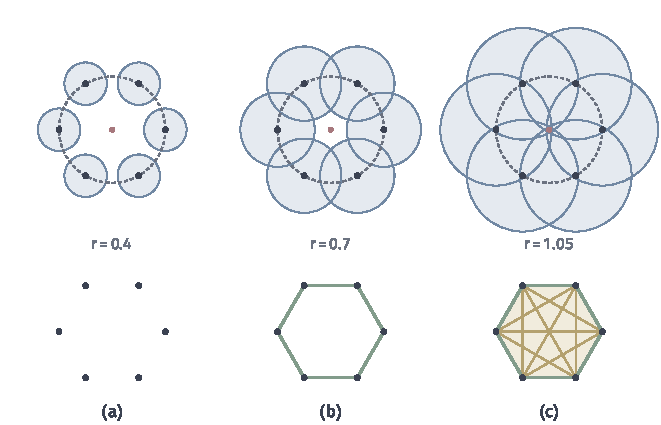
\includegraphics[width=112mm]{figures/04-spaces-measures-and-geometry/04-manifolds/matplotlib/mrec-hexagon/figure.pdf}
  \caption{单位圆上正六边形样本的球并（第一行）与对应的Čech复形（第二行）。虚线是单位圆，红点是圆心。(a) 六个球互不相交，复形只有六个顶点。(b) 相邻的球交叠成环，圆心未被覆盖，复形是六边形的边界。(c) 每个球都含圆心，复形的所有子集都是单纯形（浅黄表示填充），洞消失。}
  \label{fig:mrec-hexagon}
\end{BookInlineFigure}

\subsection{Čech复形}
\label{sec:mrec-cech}

球并是连续空间，不能直接放进计算机。它的拓扑由球与球怎样交叠决定，而交叠关系是有限的组合数据：哪些球两两相交，哪些三个球有公共点，等等。

\begin{definition}[Čech复形]
\label{def:mrec-cech}
给定欧氏空间中的有限点集$P$与半径$r>0$，\term{Čech复形}（Čech complex）$\check C_r(P)$由所有满足$\bigcap_{\bm p\in\sigma}B(\bm p,r)\neq\varnothing$的非空子集$\sigma\subseteq P$组成，其中$B(\bm p,r)$是开球。
\end{definition}

若一组球有公共点，其中任意几个球也有，所以$\check C_r(P)$对取子集封闭，是第~\ref{chap:homology}章意义下的抽象单纯复形。条件$\bigcap_{\bm p\in\sigma}B(\bm p,r)\neq\varnothing$等价于存在一点到$\sigma$中每个点的距离都小于$r$，即覆盖$\sigma$的最小闭球半径小于$r$。特别地，两点连边当且仅当它们的距离小于$2r$。

Čech复形记录的是整个球族的交叠，不只是两两的交叠。取边长为$0.9$的正三角形，$r=0.5$，如图~\ref{fig:mrec-cech-rips}。三对球两两相交，因为$0.9<1$；但覆盖三个顶点的最小球是外接球，半径
\[
 \frac{0.9}{\sqrt3}\approx0.520>0.5,
\]
三个球没有公共点。所以$\check C_{0.5}$只有三条边，没有三角形，留下一个一维的环；$r$增大到超过$0.520$时三角形被填上，环随之消失。$r\leq r'$时$\check C_r\subseteq\check C_{r'}$，尺度变化改变的正是这种填充关系。

回到正六边形，把顶点依次编号为$0,\ldots,5$。$\tfrac12<r\leq\tfrac{\sqrt3}2$时复形是六边形的边界。$r$超过$\tfrac{\sqrt3}2$后，隔一个顶点的两点连边，三个相邻顶点组成的三角形也被填上，但这些三角形都贴着外圈，中间的洞还在；直到$r>1$时，含对径点的单纯形和三角形$\{0,2,4\}$、$\{1,3,5\}$才出现，把洞填上。复形的同调与球并的同调随$r$同步变化，这不是巧合，第~\ref{sec:mrec-nerve-lemma}节解释原因。

\subsection{Rips复形}
\label{sec:mrec-rips}

判断三个以上的球有没有公共点，需要计算最小覆盖球，在高维中代价不小，而且要用到点的坐标。只用成对距离的替代方案是Rips复形。

\begin{definition}[Rips复形]
\label{def:mrec-rips}
给定有限点集$P$与它们之间的距离，以及$r>0$，\term{Rips复形}（Vietoris--Rips complex）$R_r(P)$由所有直径不超过$r$的非空子集$\sigma\subseteq P$组成，即$\sigma$中任意两点的距离都不超过$r$。
\end{definition}

判定一个单纯形只需要它各顶点之间的成对距离，所以Rips复形可以直接由距离表构造，不需要坐标，也不需要距离来自欧氏点。它由边完全确定：一组顶点构成单纯形，当且仅当其中两两之间都有边。这既是计算上的便利，也意味着它丢失了“成对相交而无公共点”的区别。

\begin{BookInlineFigure}
  \centering
  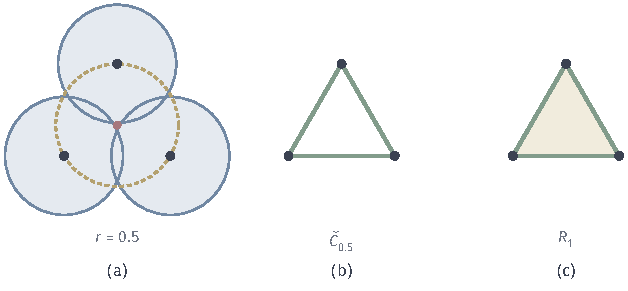
\includegraphics[width=106.299mm]{figures/04-spaces-measures-and-geometry/04-manifolds/tikz/mrec-cech-rips/figure.pdf}
  \caption{边长$0.9$的正三角形。(a) 半径$0.5$的三个球两两相交，但没有公共点；虚线是半径约$0.520$的外接圆，圆心（红）在三个开球之外。(b) Čech复形$\check C_{0.5}$只有三条边，中间是空的。(c) Rips复形$R_1$只看成对距离，三边都不超过$1$，三角形被填上。}
  \label{fig:mrec-cech-rips}
\end{BookInlineFigure}

比较两种复形时，要注意参数的含义不同：Čech复形的$r$是开球半径，Rips复形的$r$是闭的直径界。在上例中，$R_1$含有那个三角形，$\check C_{0.5}$不含，二者连边的条件几乎相同，却不是同一个复形。两者之间有如下的夹逼关系：对任意$\eta>0$，
\begin{equation}
 \check C_r(P)\subseteq R_{2r}(P)\subseteq\check C_{2r+\eta}(P).
 \label{eq:mrec-cech-rips}
\end{equation}

第一个包含：若$\sigma$中各点到某个$\bm z$的距离都小于$r$，则任意两点距离小于$2r$。第二个包含：若$\sigma$的直径不超过$2r$，取$\sigma$中任一顶点作为公共点，它到其余顶点的距离不超过$2r<2r+\eta$。这些常数足以使用，但不是最紧的。夹逼关系说明两种复形在尺度相差一倍的范围内相互控制，不能在同一个数值参数下直接等同。

\subsection{神经引理}
\label{sec:mrec-nerve-lemma}

Čech复形是球并的组合记录，现在要说明这一记录没有丢失同伦信息。一般地，给定一族集合，可以只记录哪些成员有公共点。

\begin{definition}[神经与良覆盖]
\label{def:mrec-nerve}
设$\mathcal U=\{U_1,\ldots,U_n\}$是一族集合。它的\term{神经}（nerve）$N(\mathcal U)$是以$\{1,\ldots,n\}$为顶点集的抽象单纯复形，非空子集$\sigma$是单纯形当且仅当$\bigcap_{i\in\sigma}U_i\neq\varnothing$。若每个非空的有限交$\bigcap_{i\in\sigma}U_i$都是可缩空间，则称$\mathcal U$为\term{良覆盖}（good cover），这里覆盖指它覆盖并集$\bigcup_iU_i$。
\end{definition}

按定义，$\check C_r(P)$就是开球族$\{B(\bm p,r)\}_{\bm p\in P}$的神经。有限个欧氏开球构成良覆盖：凸集的交仍是凸集，非空凸集$K$可以沿直线收缩到其中一点$\bm z_0$，同伦取
\[
 H(\bm x,t)=(1-t)\bm x+t\bm z_0 ,
\]
凸性保证$H(\bm x,t)\in K$，所以$K$可缩。

\begin{theorem}[神经引理]
\label{thm:mrec-nerve-lemma}
设$\mathcal U$是$\mathbb R^D$中有限个开凸集组成的族，则神经的几何实现$\lvert N(\mathcal U)\rvert$与并集$\bigcup_iU_i$同伦等价。特别地，对有限点集$P$和任意$r>0$，$\lvert\check C_r(P)\rvert$与球并$U_r$同伦等价。
\end{theorem}

完整的证明较长，读者可查阅Hatcher《代数拓扑》中关于神经的推论。这里构造两个方向的映射，并验证其中一个复合同伦于恒等映射，这已经能看出凸性起的作用。

从并集到神经：取一组连续函数$\varphi_i\geq0$，在$U_i$内为正、在$U_i$外为零，且处处$\sum_i\varphi_i=1$，例如把$\bm x$到$U_i$补集的距离归一化。令$F(\bm x)=\sum_i\varphi_i(\bm x)\bm v_i$，$\bm v_i$是第$i$个顶点。$\varphi_i(\bm x)>0$的那些$i$对应的集合都含$\bm x$，有公共点，所以$F(\bm x)$落在神经中的一个单纯形内。

反方向，在每个非空交$\bigcap_{i\in\sigma}U_i$中取一点$\bm c_\sigma$，在$\lvert N(\mathcal U)\rvert$的重心细分上，把$\sigma$的重心送到$\bm c_\sigma$，再在细分的每个单纯形上线性延拓，得到$G$。细分中的单纯形对应一串$\sigma_0\subseteq\cdots\subseteq\sigma_k$，所有$\bm c_{\sigma_j}$都在凸集$\bigcap_{i\in\sigma_0}U_i$中，所以$G$的像落在并集内。

现在看$G\circ F\simeq\mathrm{id}$。设$F(\bm x)$落在细分单纯形$\sigma_0\subseteq\cdots\subseteq\sigma_k$内，此时$\sigma_k$中的每个集合都含$\bm x$，特别是$\sigma_0$中的每个集合都含$\bm x$。于是$\bm x$与$G(F(\bm x))$都在凸集$\bigcap_{i\in\sigma_0}U_i$中，连接它们的线段也在其中，直线同伦$(1-t)\bm x+tG(F(\bm x))$就留在并集内。

另一个复合$F\circ G$同伦于恒等映射，这一步要复杂得多，需要在神经上逐层构造同伦，完整的论证见上面所指的文献。

神经引理把连续空间的问题转为有限计算。由第~\ref{chap:homology}章的同伦不变性，同伦等价的空间有同构的同调，几何实现的同调又等于单纯同调，于是
\begin{equation}
 H_k(U_r)\cong H_k\bigl(\lvert\check C_r(P)\rvert\bigr)\cong H_k\bigl(\check C_r(P)\bigr),
 \label{eq:mrec-nerve-homology}
\end{equation}
右端只需写出$\check C_r(P)$的边界矩阵并计算秩。正六边形的例子正是这样：$\tfrac12<r\leq\tfrac{\sqrt3}2$时，复形是六个顶点、六条边的环，边界矩阵的秩为$5$，$\beta_1=6-5=1$，与球并的环对应。

\subsection{恢复尺度}
\label{sec:mrec-recovery-scale}

至此，球并的同调可以由Čech复形算出。剩下的问题是：球并的同调何时等于$M$的同调？回到第~\ref{sec:mrec-ball-union}节的六边形，半径太小时球并断开，太大时洞被填掉，需要一个既不太小也不太大的半径。

\paragraph{两类条件}

第一类条件是覆盖：$M\subseteq U_r$，否则流形上未被覆盖的部分会让球并断开或多出洞。若样本是$\delta$稠密的，$r\geq\delta$即可。

第二类条件是不错误地连接或填充：球并不能把流形相距较远的部分接起来，也不能把流形围出的洞盖住。由于球心都在$M$上，$U_r$中每一点到$M$的距离小于$r$；若$r<\tau$，$U_r\subseteq M^\tau$，最近点投影$\pi$在整个$U_r$上有定义。

两类条件写成同一个半径的允许范围：$r$要大于某个由覆盖精度决定的下界，又要小于某个由可达半径决定的上界。只有覆盖精度相对可达半径足够小时，这个范围才非空。只看样本很密，或只看球并连通，都推不出恢复：六边形样本在$r=1.01$时球并连通且包含圆，同调却已与圆不同。

\paragraph{形变收缩的前提}

要证明$U_r$与$M$有同样的同调，最自然的方法是把$U_r$形变收缩到$M$上：令
\begin{equation}
 F(\bm x,t)=(1-t)\bm x+t\,\pi(\bm x),
 \label{eq:mrec-retraction}
\end{equation}
把每一点沿直线推向它的最近点，如图~\ref{fig:mrec-retraction}(a)。$t=0$时是恒等映射，$t=1$时落在$M$上，$M$上的点始终不动。第~\ref{chap:homology}章说明形变收缩是同伦等价。

这一构造需要两个前提。一是$\pi$在$U_r$上有定义且连续，由$r<\tau$保证。二是从$\bm x$到$\pi(\bm x)$的线段整个留在$U_r$中，否则$F$会离开$U_r$，不是$U_r$上的形变。第二个前提并不平凡：线段从$\bm x$所在的球出发，它的另一端$\pi(\bm x)$可能落在别的球里，中间不能经过球并之外的缝隙。下一小节的证明处理的就是这件事。

\paragraph{圆上的核对}

单位圆的可达半径为$\tau=1$。下一小节的定理要求样本是$\varepsilon/2$稠密的，且$\varepsilon<\sqrt{3/5}\,\tau\approx0.775$，所以覆盖精度必须小于约$0.387$。

正六边形的覆盖精度是$0.518$，不满足条件。尽管如此，$r=0.6$时球并覆盖了圆，又没有盖住圆心，同调仍然正确；定理的条件是充分的，不是必要的。

改取$24$个等距样本，覆盖精度为$0.131$。允许的半径范围是$2\times0.131<\varepsilon<0.775$，例如$\varepsilon=0.3$，图~\ref{fig:mrec-retraction}(a)画的就是这个球并。在这个范围内，定理保证球并的同调等于圆的同调，即$\beta_0=\beta_1=1$。

\subsection{同调恢复定理}
\label{sec:mrec-homology-theorem}

把上面的条件定量化，就得到Niyogi、Smale与Weinberger的结果。

\begin{theorem}[有限样本的同调恢复]
\label{thm:mrec-homology-recovery}
设$M\subseteq\mathbb R^D$是紧致无边界的光滑嵌入子流形，可达半径为$\tau>0$。设有限样本$P\subseteq M$是$\varepsilon/2$稠密的，即$M$上每一点到最近样本的环境距离小于$\varepsilon/2$，且$0<\varepsilon<\sqrt{3/5}\,\tau$。则式~\eqref{eq:mrec-ball-union}的球并$U_\varepsilon$形变收缩到$M$，从而对每个$k$，
\begin{equation}
 H_k(M)\cong H_k(U_\varepsilon)\cong H_k\bigl(\check C_\varepsilon(P)\bigr).
 \label{eq:mrec-homology-recovery}
\end{equation}
\end{theorem}

证明的关键是说明线段$[\bm x,\pi(\bm x)]$留在球并中。思路是分两种情形：要么$\pi(\bm x)$就在$\bm x$所在的球内，线段自然留在这个凸的球里；要么$\pi(\bm x)$离球心较远，这时可以证明$\bm x$离流形很近，于是整条线段都落在$\pi(\bm x)$附近某个样本的球里，如图~\ref{fig:mrec-retraction}(b)。

\begin{proof}
由$\varepsilon/2$稠密，$M\subseteq U_\varepsilon$。由$\varepsilon<\tau$，$U_\varepsilon\subseteq M^\tau$，$\pi$在$U_\varepsilon$上连续。下面证明对任一$\bm x\in U_\varepsilon$，线段$[\bm x,\pi(\bm x)]$留在$U_\varepsilon$中。

设$\bm x\in B(\bm p,\varepsilon)$，$\bm p\in P$。记$\bm q=\pi(\bm x)$，并记
\[
 T=\lVert\bm x-\bm q\rVert_2,\qquad a=\lVert\bm p-\bm q\rVert_2 .
\]
$T=0$时无需证明。否则令$\bm v=(\bm x-\bm q)/T$，由一阶条件它是$\bm q$处的单位法向量。$\bm q$是最近点，所以
\[
 T\leq\lVert\bm x-\bm p\rVert_2<\varepsilon<\tau .
\]

情形一，$a<\varepsilon$。此时$\bm x,\bm q$都在开球$B(\bm p,\varepsilon)$中，球是凸的，线段留在其中。

情形二，$a\geq\varepsilon$。先估计$T$。由$\bm x-\bm p=(\bm q-\bm p)+T\bm v$，
\[
 \lVert\bm x-\bm p\rVert_2^2=a^2+T^2-2T\langle\bm p-\bm q,\bm v\rangle .
\]
由式~\eqref{eq:mrec-reach-normal}，$\langle\bm p-\bm q,\bm v\rangle\leq a^2/(2\tau)$，代入并用$\lVert\bm x-\bm p\rVert_2<\varepsilon$，得
\[
 \varepsilon^2>a^2\Bigl(1-\frac T\tau\Bigr)+T^2 .
\]
因为$T<\tau$，右端对$a$递增，代入$a\geq\varepsilon$，得$\varepsilon^2>\varepsilon^2(1-T/\tau)+T^2$，整理后
\begin{equation}
 T<\frac{\varepsilon^2}\tau .
 \label{eq:mrec-t-bound}
\end{equation}

再取样本$\bm q'$使$b=\lVert\bm q-\bm q'\rVert_2<\varepsilon/2$，这由稠密性保证。线段上的点可写成$\bm y=\bm q+t\bm v$，$0\leq t\leq T$。展开$\lVert\bm y-\bm q'\rVert_2^2$，并对$\bm q'-\bm q$的法向分量用式~\eqref{eq:mrec-reach-normal}，得
\[
 \lVert\bm y-\bm q'\rVert_2^2\leq b^2+t^2+\frac{tb^2}\tau .
\]
代入$b^2<\varepsilon^2/4$和式~\eqref{eq:mrec-t-bound}，
\[
 \lVert\bm y-\bm q'\rVert_2^2<\frac{\varepsilon^2}4+\frac{\varepsilon^4}{\tau^2}+\frac{\varepsilon^4}{4\tau^2}=\frac{\varepsilon^2}4+\frac54\cdot\frac{\varepsilon^4}{\tau^2}.
\]
由$\varepsilon^2<\tfrac35\tau^2$，第二项小于$\tfrac34\varepsilon^2$，于是$\lVert\bm y-\bm q'\rVert_2<\varepsilon$。整条线段都在球$B(\bm q',\varepsilon)$中。

这样，式~\eqref{eq:mrec-retraction}定义的$F$就是$U_\varepsilon$到$M$的形变收缩：它连续，$t=0$时是恒等映射，$t=1$时映入$M$，且保持$M$上的点不动。所以$M\hookrightarrow U_\varepsilon$是同伦等价，第一个同构成立。第二个同构是式~\eqref{eq:mrec-nerve-homology}。
\end{proof}

常数$\sqrt{3/5}$的来源就在这个证明里：它恰好使$\tfrac14+\tfrac54(\varepsilon/\tau)^2<1$。右端是有限复形的单纯同调，可以由边界矩阵的秩算出，这就是“由有限样本恢复同调”的含义。

\begin{BookInlineFigure}
  \centering
  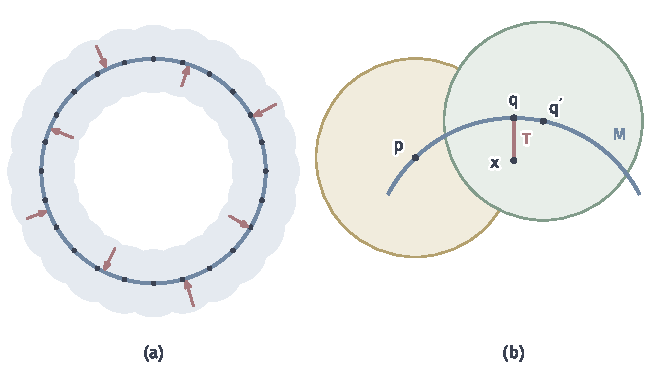
\includegraphics[width=112mm]{figures/04-spaces-measures-and-geometry/04-manifolds/matplotlib/mrec-retraction/figure.pdf}
  \caption{球并向流形的形变收缩。(a) 单位圆上$24$个等距样本、$\varepsilon=0.3$的球并（浅蓝），红色箭头把点沿线段推向最近点。(b) 证明情形二的几何（$\tau=1$，$\varepsilon=0.7$）：$\bm x$在$\bm p$的球（浅黄）中，但最近点$\bm q$不在其中；此时$T<\varepsilon^2/\tau$，线段$[\bm x,\bm q]$整条落在靠近$\bm q$的样本$\bm q'$的球（浅绿）中。}
  \label{fig:mrec-retraction}
\end{BookInlineFigure}

\paragraph{恢复的是什么}

定理恢复的是同调，而且是经由同伦等价得到的。它不给出与$M$同胚的空间：$U_\varepsilon$是$\mathbb R^D$中的开集，维数是$D$而不是$m$，与$M$同伦等价却不同胚；$\check C_\varepsilon(P)$可以含有维数远高于$m$的单纯形。至于$M$的光滑结构、度量或嵌入方式，定理没有给出任何信息。

定理的条件也划定了它的适用范围。样本必须在$M$上：观测离开流形时，需要把扰动界与覆盖精度、可达半径一起放进新的条件，并重新证明形变收缩。定理用的是Čech复形：改用Rips复形时，只能借助式~\eqref{eq:mrec-cech-rips}，在相差一倍的两个尺度之间比较，需要另行论证。从同调进一步恢复同胚类型，则需要完全不同的工具。

\section{持久同调}
\label{sec:mrec-persistence}

同调恢复定理要求半径落在一个由覆盖精度和可达半径决定的范围内，而这两个量通常并不知道，实际中只能尝试许多半径。逐个半径地报告Betti数会丢掉一个重要的信息：某个尺度下的一个环，与稍大尺度下的一个环，是不是同一个环。

可以把这件事想象成涨潮时看海岸：每个时刻拍一张照片，只数岛屿的个数，并不知道这个时刻的岛屿和下一时刻的岛屿谁是谁；若把录像连起来看，就能说清楚每个岛何时露出、何时被淹。本节让复形随尺度嵌套增长，用包含诱导的线性映射追踪同调类，得到的表示称为\term{持久同调}（persistent homology）。随后研究这一表示对距离扰动的稳定性，并说明它与第~\ref{sec:mrec-homology-recovery}节的恢复保证是两回事。

\subsection{过滤与诱导映射}
\label{sec:mrec-filtration}

Čech复形与Rips复形都随尺度单调增长：$r\leq r'$时$\check C_r(P)\subseteq\check C_{r'}(P)$，$R_r(P)\subseteq R_{r'}(P)$。

\begin{definition}[过滤]
\label{def:mrec-filtration}
一族以实数$r\geq0$为指标的单纯复形$\{K_r\}$，若$r\leq r'$时$K_r$是$K_{r'}$的子复形，则称为一个\term{过滤}（filtration）。
\end{definition}

对有限点集，Rips过滤只在有限个尺度上发生变化，这些尺度是成对距离的取值；Čech过滤的变化尺度是各子集最小覆盖球的半径，也只有有限个。两个相邻变化尺度之间，复形保持不变。

对每个$r\leq r'$，包含$K_r\hookrightarrow K_{r'}$诱导线性映射
\begin{equation}
 f_{r,r'}:H_k(K_r)\to H_k(K_{r'}),
 \label{eq:mrec-induced-map}
\end{equation}
这里同调取实系数。第~\ref{chap:homology}章说明，恒等包含诱导恒等映射，两次包含的复合诱导映射的复合，所以$f_{r,r}$是恒等映射，并且$f_{r',r''}\circ f_{r,r'}=f_{r,r''}$。这一族线性空间与线性映射称为一个\term{持久模}（persistence module）。

\paragraph{过滤的例子}

取边长为$1$的正方形的四个顶点作Rips过滤，如图~\ref{fig:mrec-filtration}(a)。$r<1$时只有四个点，$\beta_0=4$。$1\leq r<\sqrt2$时四条边出现，组成一个四边形，$\beta_0=1$，$\beta_1=1$。$r\geq\sqrt2$时两条对角线出现，四个三角形和整个四面体随之加入，复形可缩，$\beta_0=1$，$\beta_1=0$。

再取数轴上的三个点$0$、$1$、$3$。$r<1$时有三个分支；$r=1$时点$0$与点$1$合并；$r=2$时点$1$与点$3$相连，只剩一个分支。映射$f_{0.5,1.5}$把点$0$与点$1$的类送到同一个类，把点$3$的类送到它自己。诱导映射记录了是哪两个分支合并，这是Betti数序列$3,2,1$所没有的。

\paragraph{Betti数不足以描述跨尺度信息}

下面两个过滤的一维Betti数在每个尺度上都相同，诱导映射却不同。这两个过滤是直接写出的抽象过滤，不必来自点集。

过滤甲：四边形$abcd$在$r=1$时出现，在$r=3$时加入一条对角线和两个三角形被填满。过滤乙：四边形$abcd$同样在$r=1$时出现，但在$r=2$时被填满，同时另一个四边形$efgh$在$r=2$出现，在$r=3$时被填满。两者的零维同调不同，下面只比较一维同调。

两者的$\beta_1$都是：$r<1$时为$0$，$1\leq r<3$时为$1$，之后为$0$。但在过滤甲中，$f_{1.5,2.5}$把$r=1.5$处的环送到$r=2.5$处的同一个环，是同构；在过滤乙中，$r=1.5$处的环在$r=2$时已被填满，$f_{1.5,2.5}=0$，$r=2.5$处的环是新出现的。只看每个尺度的Betti数，无法区分“一个环持续存在”与“一个环消失、另一个环出现”。

\begin{BookInlineFigure}
  \centering
  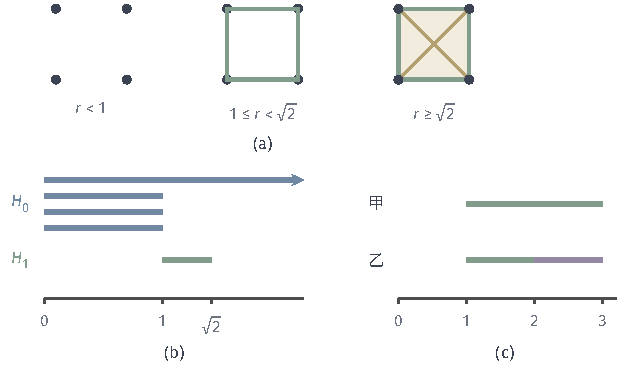
\includegraphics[width=105.346mm]{figures/04-spaces-measures-and-geometry/04-manifolds/tikz/mrec-filtration/figure.pdf}
  \caption{过滤与条形码。(a) 单位正方形的Rips过滤的三个阶段，浅黄表示填充的单纯形。(b) 正方形的条形码，蓝条是$H_0$（一根永不消失），绿条是$H_1$。(c) 过滤甲与过滤乙的$H_1$：逐尺度的Betti数相同，甲是一根贯穿的条，乙是前后相接的两根（绿、紫）。}
  \label{fig:mrec-filtration}
\end{BookInlineFigure}

\subsection{区间分解}
\label{sec:mrec-interval-decomposition}

持久模看起来是一串空间和映射，结构复杂。对有限点产生的过滤，它其实可以完全拆成最简单的块，每一块描述一个同调类从出现到消失的区间。

\paragraph{区间模与分解定理}

固定同调次数$k$。设$b<d\leq+\infty$，\term{区间模}（interval module）$I[b,d)$在$r\in[b,d)$处取$\mathbb R$，其余处取零空间；当$r\leq r'$都在$[b,d)$中时，映射是恒等映射，其余映射为零。它描述的正是一个在尺度$b$出现、在尺度$d$消失的同调类。

\begin{theorem}[区间分解]
\label{thm:mrec-interval-decomposition}
设过滤$\{K_r\}$由有限个复形组成，只在有限个尺度上变化，每个$K_r$都是有限复形。则对每个$k$，持久模$\{H_k(K_r),f_{r,r'}\}$同构于有限个区间模的直和$\bigoplus_lI[b_l,d_l)$，并且区间的多重集合$\{[b_l,d_l)\}$由持久模唯一确定。
\end{theorem}

证明要在所有尺度上同时选取相容的基，用到有限维空间中两个子空间族存在公共基的引理，篇幅较长，读者可查阅Zomorodian与Carlsson关于持久同调计算的论文。

结论的含义可以这样理解。可以在所有尺度上选取相容的基，使每个诱导映射都把基向量送到基向量或零。一个基向量对应一个区间，它出现的尺度是左端点，被送到零的尺度是右端点。这就像把线性映射化成对角形，只不过这里是一整串映射同时化简。两个分支合并时，约定保留出现较早的那个，较晚的那个记为消失，这一约定保证了分解的一致性。

由分解立刻得到一个常用的计数：$r\leq r'$时，$f_{r,r'}$的秩等于同时包含$r$和$r'$的区间的个数。

\paragraph{条形码与持久图}

区间的多重集合称为\term{条形码}（barcode），每个区间画成一根横条。也可以把每个区间$[b,d)$画成平面上的点$(b,d)$，分别称为出生坐标与死亡坐标，得到\term{持久图}（persistence diagram）；所有点都在对角线$b=d$上方，$d=+\infty$的点画在顶端。

端点的约定要说清。Rips过滤用闭条件，区间取左闭右开：类在尺度$b$已经存在，在尺度$d$恰好变为零或并入更早的类。Čech过滤用开球，单纯形在$r$严格超过阈值时才出现，区间实际是左开右闭的$(b,d]$，这只影响端点本身，不影响区间的长度和配对。不会在有限尺度消失的类对应$d=+\infty$，要保留在图中。

上一小节的例子可以直接读出条形码。正方形：$H_0$为$[0,\infty)$与三个$[0,1)$，$H_1$为$[1,\sqrt2)$。数轴上的三点：$H_0$为$[0,\infty)$、$[0,1)$、$[0,2)$。过滤甲的$H_1$为$[1,3)$，过滤乙的$H_1$为$[1,2)$与$[2,3)$，两者的区别清楚地显示出来，如图~\ref{fig:mrec-filtration}(b)(c)。

正六边形给出一个更有启发的比较。Rips过滤在$r=1$时出现六边形的环；$r=\sqrt3$时加入隔一个顶点的边，八个三角形恰好围成八面体的表面，环被填上，同时出现一个二维的空腔；$r=2$时加入对径的边，复形成为实心单纯形，空腔消失。所以$H_1$为$[1,\sqrt3)$，$H_2$为$[\sqrt3,2)$，见图~\ref{fig:mrec-barcodes}(a)。

Čech过滤的情形不同。由神经引理，它与平面中的球并同伦等价，而平面开集没有二维同调，所以没有$H_2$的条，$H_1$只有$(\tfrac12,1]$，见图~\ref{fig:mrec-barcodes}(b)。Rips过滤多出来的那根$H_2$条，正是它“成对相交就算有公共点”造成的，并不反映任何真实的二维结构。

条形码是跨尺度同调的表示，它不记录点的坐标，也不记录同胚类型或光滑结构。两组完全不同的点可以有相同的条形码，例如把整组点作任意合同变换，Rips过滤不变。

\begin{BookInlineFigure}
  \centering
  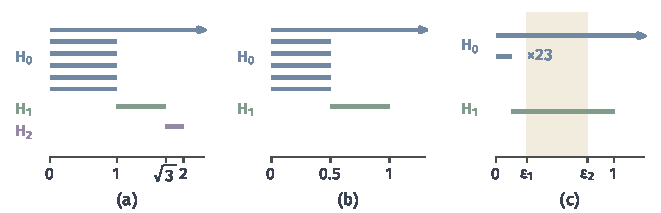
\includegraphics[width=112mm]{figures/04-spaces-measures-and-geometry/04-manifolds/matplotlib/mrec-barcodes/figure.pdf}
  \caption{由边界矩阵算出的条形码，横轴为尺度。(a) 单位正六边形的Rips过滤，$H_2$的条是八面体空腔。(b) 同一组点的Čech过滤，横轴为球半径，没有$H_2$。(c) 单位圆上$24$个等距样本的Čech过滤，$H_0$有$23$根相同的短条，$H_1$的唯一长条横跨浅黄色的恢复窗口$(\varepsilon_1,\varepsilon_2)$。}
  \label{fig:mrec-barcodes}
\end{BookInlineFigure}

\subsection{瓶颈距离}
\label{sec:mrec-bottleneck}

要谈条形码的稳定性，先要能比较两张持久图。数据稍有变化，长条的端点应该稍有移动，同时可能冒出或消失一些很短的条。比较时应把长条与长条配对，短条则允许与“无”配对，代价是它本身的长度。

\begin{definition}[瓶颈距离]
\label{def:mrec-bottleneck}
固定同调次数，设$D_1,D_2$是两张持久图，即点$(b,d)$的有限多重集合。部分匹配是$D_1$与$D_2$之间的一个部分双射，未被匹配的点改为与对角线匹配。匹配的点对$(b,d)$与$(b',d')$的代价为$\max(\lvert b-b'\rvert,\lvert d-d'\rvert)$，与对角线匹配的点$(b,d)$的代价为$(d-b)/2$。\term{瓶颈距离}（bottleneck distance）$d_B(D_1,D_2)$是全部部分匹配中最大代价的最小值。
\end{definition}

点$(b,d)$到对角线的$L^\infty$距离恰为$(d-b)/2$，所以与对角线匹配就是把点移到最近的对角线位置，如图~\ref{fig:mrec-diagram}(a)。死亡坐标为$+\infty$的点，只能与死亡坐标同为$+\infty$的点匹配，代价取$\lvert b-b'\rvert$；两张图中这类点个数不同时，瓶颈距离为$+\infty$。

\begin{example}[两张一维持久图]
\label{ex:mrec-bottleneck}
考虑下面两张持久图：
\[
 D_1=\{(1,3)\},\qquad D_2=\{(1.2,2.9),\ (2,2.2)\}.
\]
把$(1,3)$与$(1.2,2.9)$匹配，代价是
\[
 \max(0.2,\ 0.1)=0.2 .
\]
把$(2,2.2)$与对角线匹配，代价是$0.1$。最大代价为$0.2$，所以$d_B\leq0.2$。

反过来，任何匹配中$(1,3)$都要有去处：与$(1.2,2.9)$匹配代价$0.2$，与$(2,2.2)$匹配代价$\max(1,0.8)=1$，与对角线匹配代价$1$。所以最大代价至少为$0.2$，于是
\[
 d_B(D_1,D_2)=0.2 .
\]
短条$(2,2.2)$只贡献了$0.1$，它的出现几乎不改变距离。
\end{example}

\begin{BookInlineFigure}
  \centering
  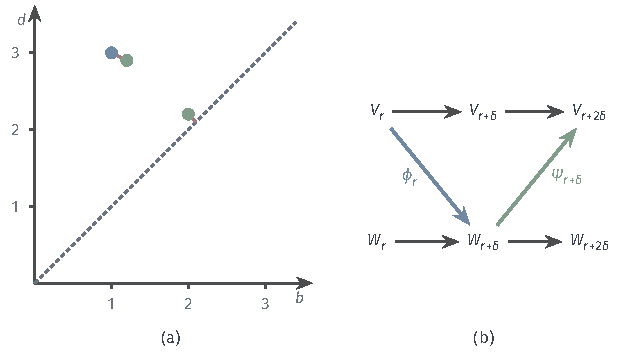
\includegraphics[width=105.184mm]{figures/04-spaces-measures-and-geometry/04-manifolds/tikz/mrec-diagram/figure.pdf}
  \caption{持久图的匹配与持久模的交错。(a) 例~\ref{ex:mrec-bottleneck}的两张持久图，$D_1$为蓝点，$D_2$为绿点，红色线段表示最优匹配，靠近对角线的绿点匹配到对角线。(b) 交错的一个片段：先走蓝色的$\phi$，再走绿色的$\psi$，结果等于沿$V$直接走$2\delta$。}
  \label{fig:mrec-diagram}
\end{BookInlineFigure}

\subsection{过滤交错}
\label{sec:mrec-interleaving}

现在比较同一组点标签上的两张距离表。设$d=[d_{i,j}]$与$d'=[d'_{i,j}]$都是对称、零对角的非负矩阵，可以来自同一组点在两次测量中的结果，并且$\lvert d_{i,j}-d'_{i,j}\rvert\leq\delta$对所有$i,j$成立。记$R_r(d)$为按距离表$d$、直径界$r$构造的Rips复形。

若$\sigma$在$R_r(d)$中，它的每对顶点满足$d_{i,j}\leq r$，从而$d'_{i,j}\leq r+\delta$，所以$\sigma$在$R_{r+\delta}(d')$中。对称地，$R_r(d')\subseteq R_{r+\delta}(d)$。于是两套过滤交替地相互包含：
\begin{equation}
 R_r(d)\subseteq R_{r+\delta}(d')\subseteq R_{r+2\delta}(d),
 \label{eq:mrec-rips-interleave-1}
\end{equation}
\begin{equation}
 R_r(d')\subseteq R_{r+\delta}(d)\subseteq R_{r+2\delta}(d').
 \label{eq:mrec-rips-interleave-2}
\end{equation}

这些复形都是同一个顶点集上全体单纯形的子复形，所有映射都是包含，所以复合的包含$R_r(d)\subseteq R_{r+2\delta}(d)$与原过滤中的推进是同一个包含，与沿过滤推进再平移的各种路径都相容。把这种“隔一步能互相换过去、并且与自身的推进相容”的关系抽象出来，就是下面的定义。

\begin{definition}[交错]
\label{def:mrec-interleaving}
设$\{V_r,v_{r,r'}\}$与$\{W_r,w_{r,r'}\}$是两个持久模，$\delta\geq0$。若存在线性映射$\phi_r:V_r\to W_{r+\delta}$与$\psi_r:W_r\to V_{r+\delta}$，它们与两个持久模自身的映射交换，并满足$\psi_{r+\delta}\circ\phi_r=v_{r,r+2\delta}$与$\phi_{r+\delta}\circ\psi_r=w_{r,r+2\delta}$，则称两个持久模$\delta$\term{交错}（interleaved）。
\end{definition}

图~\ref{fig:mrec-diagram}(b)画的是其中一个等式：沿蓝、绿两条斜线走到$V_{r+2\delta}$，与沿上面一行直接走是同一个映射。对两套Rips过滤取$k$维同调，式~\eqref{eq:mrec-rips-interleave-1}和式~\eqref{eq:mrec-rips-interleave-2}的包含诱导出$\phi_r$与$\psi_r$；包含的复合等于包含，诱导映射的复合也就等于诱导映射，定义中的等式全部成立。所以两个持久模$\delta$交错。

交错为什么能控制条形码？下面的不等式给出最直接的一步。

\begin{lemma}[秩的比较]
\label{lem:mrec-rank-interleaving}
设两个持久模$\delta$交错，$r+2\delta\leq r'$，则
\begin{equation}
 \operatorname{rank}v_{r,r'}\leq\operatorname{rank}w_{r+\delta,r'-\delta}.
 \label{eq:mrec-rank-interleaving}
\end{equation}
\end{lemma}
\begin{proof}
由交错的定义，$v_{r,r'}$可以分解为
\[
 V_r\xrightarrow{\ \phi_r\ }W_{r+\delta}\xrightarrow{\ w\ }W_{r'-\delta}\xrightarrow{\ \psi_{r'-\delta}\ }V_{r'} .
\]
事实上，$\phi$与两个持久模自身的映射交换，所以
\[
 w_{r+\delta,r'-\delta}\circ\phi_r=\phi_{r'-2\delta}\circ v_{r,r'-2\delta}.
\]
再用交错定义中的等式，
\[
 \psi_{r'-\delta}\circ\phi_{r'-2\delta}=v_{r'-2\delta,r'} ,
\]
就得到$v_{r,r'}$。复合映射的秩不超过中间映射的秩。
\end{proof}

由区间分解后的计数，式~\eqref{eq:mrec-rank-interleaving}说：$V$中覆盖$[r,r']$的条的根数，不超过$W$中覆盖$[r+\delta,r'-\delta]$的条的根数。这正是“一根条在对方那里有一根端点相差不超过$\delta$的对应条”的计数形式。把这些计数不等式对所有$r,r'$合起来，再用组合匹配的论证，就能得到下面的定理。

\begin{theorem}[持久图的稳定性]
\label{thm:mrec-stability}
设两个持久模的每个空间都是有限维的，并且它们$\delta$交错，则它们的持久图的瓶颈距离不超过$\delta$。特别地，若两张距离表逐项之差不超过$\delta$，则对每个$k$，两套Rips过滤的$k$维持久图满足$d_B\leq\delta$。
\end{theorem}

这一结果称为代数稳定性定理，从计数不等式到匹配的证明较长，读者可查阅Chazal等人关于持久模稳定性的论文。

它的作用是把几何上的扰动换成表示上的扰动。例如每个点移动不超过$\eta$，成对距离至多改变$2\eta$，持久图在瓶颈距离下至多移动$2\eta$。长于$4\eta$的条不会因此消失，只是端点稍有移动；短于这个量的条则可能出现或消失。

定理控制的只是表示的变化。它说两次测量得到的持久图相近，却没有说任何一张持久图反映了底层流形的同调：两张距离表都可能来自采样不足的数据，它们的条形码彼此接近，同时都与流形无关。

\subsection{持久信息的解释}
\label{sec:mrec-persistence-interpretation}

把持久同调与第~\ref{sec:mrec-homology-recovery}节的恢复定理放在一起，可以分清哪些结论有保证。设样本$P\subseteq M$的覆盖精度$\delta_P$满足
\begin{equation}
 2\delta_P<\varepsilon_1<\varepsilon_2<\sqrt{3/5}\,\tau ,
 \label{eq:mrec-recovery-window}
\end{equation}
则区间$[\varepsilon_1,\varepsilon_2]$中的每个$\varepsilon$都满足定理~\ref{thm:mrec-homology-recovery}的条件，称它为恢复窗口。

\paragraph{窗口内的条}

对窗口中的$\varepsilon\leq\varepsilon'$，包含$j:U_\varepsilon\hookrightarrow U_{\varepsilon'}$是同伦等价。理由如下：记$i:M\hookrightarrow U_\varepsilon$、$i':M\hookrightarrow U_{\varepsilon'}$，二者都是同伦等价，且$j\circ i=i'$；取$i$的同伦逆$h$，则
\[
 j\simeq j\circ i\circ h=i'\circ h,
\]
是同伦等价的复合。所以$H_k(U_\varepsilon)\to H_k(U_{\varepsilon'})$是同构。

进一步可以证明，神经引理中的同伦等价能与包含相容地选取，这要求把神经引理的证明做成对包含自然的形式，读者可查阅Chazal与Oudot关于持久性重建的论文。于是Čech过滤在窗口内的诱导映射都是同构。由区间分解，没有区间的端点落在窗口内部，凡是与窗口相交的条都横跨整个窗口，并且这样的$k$维条恰有$\beta_k(M)$根。这是已经建立了恢复保证的结论。

单位圆上$24$个等距样本的例子可以把这件事算到底。条件给出窗口$\varepsilon_1=2\delta_P\approx0.262$到$\varepsilon_2\approx0.775$。Čech过滤中，相邻两球在$r$超过弦长的一半$\approx0.131$时相交，圆环在此形成；圆心在$r$超过$1$时才被覆盖。所以$H_1$唯一的条是$(0.131,1]$，它横跨窗口，根数$1=\beta_1(S^1)$；$H_0$除了永不消失的条，$23$根短条都在$0.131$处结束，在窗口之前，见图~\ref{fig:mrec-barcodes}(c)。

\paragraph{窗口外的条}

窗口外的条没有这样的保证。很靠近$0$的短条通常反映采样的离散性，很大尺度上的条则反映样本整体的粗略形状，它们与$M$的关系都没有经过论证。更重要的是，实际中并不知道$\delta_P$和$\tau$，也就不知道窗口在哪里，甚至不知道窗口是否存在。

没有覆盖、噪声和几何尺度的条件时，寿命长只表示同调类跨越很大的尺度范围而持续存在。一个例子是：底层集合是一个实心圆盘，没有洞，但样本只取在它的边界圆附近。Rips过滤会给出一根很长的一维条，它如实地反映了样本的形状，却不是圆盘的孔洞；问题出在样本没有覆盖圆盘内部，任何对持久图的处理都无法补上未被采样的区域。

\paragraph{其他过滤与噪声}

上面的结论是对样本在流形上的Čech过滤建立的。对Rips过滤，只能借助式~\eqref{eq:mrec-cech-rips}的夹逼关系，把恢复窗口中的信息传过来，这要求窗口跨越一倍以上的尺度，需要另行论证；正六边形的$H_2$条提醒我们，Rips过滤确实可能给出流形中不存在的同调。观测离开流形时，恢复窗口本身需要重新建立。

表示的稳定性也不能单独证明真实孔洞的存在：定理~\ref{thm:mrec-stability}保证小扰动不会让长条消失，但长条从哪里来，要由覆盖、噪声和可达半径的条件回答。持久同调提供的是跨尺度的完整记录及其稳定性，它与恢复保证配合使用，不能替代后者。

\section{本章小结}
\label{sec:mrec-summary}

本章开头问：只凭有限个样本，能否知道一个未知流形在各点朝哪个方向、局部长什么样、沿它走有多远、有几个分支和几个洞。回答的前提是一个共同的采样模型。覆盖精度说明流形上有没有远离样本的地方，扰动界说明观测离开流形多远，可达半径同时度量流形在环境中的弯曲以及不同部分相互接近的程度，并保证不同分支至少相隔$2\tau$。这些量是分析的假设，不能从样本中准确读出；全域稠密也不保证每个邻域内样本在各切向上都有展开。

可达半径有两条局部推论。半径为$\tau$的球能贴着流形滚动，由此得到流形偏离切平面的二次界；对弦的中点反复投影，得到内在距离与弦长的比较。后面每一节都用到它们。

局部几何的恢复建立在切向近似上。局部PCA用邻域协方差的主方向估计切空间，它最小化到子空间的平方距离和；把弯曲与扰动写进协方差的扰动，由谱隙界得到方向误差，弯曲项随邻域半径增大、噪声项随半径减小，两者都依赖样本在切向上的展开程度。在估计的平面上用含常数项、一次项与二次项的多项式拟合法向分量，就得到连续的局部片；函数值误差不控制导数，多片的并也不自动是流形。

内在距离由邻域图上的最短路逼近。只要覆盖精度小于半径的一半、半径小于$2\tau$，图距离与内在距离之比就夹在两个因子之间，分别由$r/\tau$与$\delta/r$决定。缺采样使图距离过大甚至断开，邻接过大使它跨越相近的部分而过小，离开流形的噪声还要求半径明显大于扰动界。

拓扑的恢复走另一条路，不依赖局部拟合。样本的球并把离散点变成连续空间，Čech复形是它的神经，有限欧氏开球构成良覆盖，神经引理使二者同伦等价，同调随之可以由边界矩阵算出。在样本$\varepsilon/2$稠密且$\varepsilon<\sqrt{3/5}\,\tau$时，每一点沿直线推向最近点的路径留在球并内，球并形变收缩到流形。这恢复的是同调，不是同胚；样本离开流形或改用Rips复形都需要另行论证。

尺度未知时，持久同调让复形随尺度增长，用包含诱导的映射追踪同调类，有限过滤的持久模分解为区间，得到条形码与持久图。两张距离表逐项相差不超过$\delta$时，两套Rips过滤$\delta$交错，持久图的瓶颈距离不超过$\delta$，这是表示的稳定性。只有在恢复窗口内，横跨窗口的条才对应流形的同调；寿命长只说明跨尺度持续，不能单独证明真实孔洞的存在。

表~\ref{tab:mrec-summary}把各条线索的输入、关键条件和输出列在一起，它们各有自己的条件和结论，不能相互替代。

\begin{BookInlineTable}
  \centering
  \caption{本章各线索的条件与结论}
  \label{tab:mrec-summary}
  \begin{tabular}{lll}
    \toprule
    线索 & 关键条件 & 结论 \\
    \midrule
    切空间估计 & $\lambda_T>0$，$\beta$相对$\lambda_T$小 & 方向误差~\eqref{eq:mrec-local-pca-error} \\
    局部片拟合 & $\bm\Phi$满列秩，图表示成立 & 系数误差~\eqref{eq:mrec-coefficient-error} \\
    内在距离 & $2\delta<r<2\tau$ & 比值界~\eqref{eq:mrec-graph-lower}、\eqref{eq:mrec-graph-upper} \\
    同调恢复 & $\varepsilon/2$稠密，$\varepsilon<\sqrt{3/5}\,\tau$ & 同构~\eqref{eq:mrec-homology-recovery} \\
    持久图稳定性 & 距离表逐项相差不超过$\delta$ & $d_B\leq\delta$ \\
    \bottomrule
  \end{tabular}
\end{BookInlineTable}

本章的条件都是确定性的：给定样本与扰动界，判断结论是否成立。样本随机抽取时这些条件以多大概率满足，属于卷八的统计问题；以拟合残差或距离畸变为目标的进一步优化，则属于卷五。


